% main.tex for MA2500

% main.tex for MA2500 Foundations of Probability and Statistics

%\PassOptionsToPackage{noproofs}{camnotes}
%\PassOptionsToPackage{noanswers}{camnotes}
%\PassOptionsToPackage{blanksolutions}{camnotes}

%------------------------------------------------
\documentclass[twoside]{book}

\usepackage{camnotes}
\usepackage{camstyle}

% module info
\institution{Cardiff University}
\department{School of Mathematics}
\modulecode{MA2500}
\moduletitle{Foundations of Probability and Statistics}
\moduleterm{Autumn 2018}

% document info
\title{Lecture Notes}
\author{D Evans}
\newcommand{\version}{\today}

% new commands
\newcommand{\Z}{\mathbb{Z}}
\newcommand{\N}{\mathbb{N}}
\newcommand{\R}{\mathbb{R}}
\newcommand{\C}{\mathbb{C}}
\newcommand{\card}{\text{card}}
\newcommand{\supp}{\text{supp}}
\newcommand{\prob}{\mathbb{P}}
\newcommand{\expe}{\mathbb{E}}
\newcommand{\var}{\text{Var}}
\newcommand{\cov}{\text{Cov}}
\newcommand{\mode}{\text{Mode}}
\newcommand{\pvalue}{p\text{-value}}
\newcommand{\lt}{<}
\newcommand{\gt}{>}
\newcommand{\bias}{\text{Bias}}
\newcommand{\mse}{\text{MSE}}
\newcommand{\stackss}[2]{\textstyle\genfrac{}{}{0pt}{}{{#1}}{{#2}}}
\newcommand{\Xbar}{\bar{X}}
\newcommand{\medcup}{{\textstyle\bigcup}}
\newcommand{\medcap}{{\textstyle\bigcap}}
\DeclareMathOperator*{\argmin}{\arg\!\min}
\DeclareMathOperator*{\argmax}{\arg\!\max}

% naughty macros
\def\it{\item}
\def\bit{\begin{itemize}}
\def\eit{\end{itemize}} 
\def\ben{\begin{enumerate}}
\def\een{\end{enumerate}}

% tweaks
\renewcommand{\emph}[1]{\textbf{#1}}
\setcounter{tocdepth}{1}
\setstretchfactor{1.75}

% more stuff
\usepackage{diagbox}
\usepackage{mathtools}
\newcommand{\transpose}[1]{{#1}^{\mathrm{T}}}
\newcommand{\boldx}{\boldsymbol{x}}
\newcommand{\boldy}{\boldsymbol{y}}
\newcommand{\boldX}{\boldsymbol{X}}
\newcommand{\boldY}{\boldsymbol{Y}}
\newcommand{\boldbeta}{\boldsymbol{\beta}}
\newcommand{\boldepsilon}{\boldsymbol{\epsilon}}
\newcommand{\odds}{\text{odds}}
\newcommand{\logodds}{\text{log-odds}}
\newcommand{\logit}{\text{logit}}

%------------------------------------------------
\begin{document}
\maketitle
\tableofcontents
\cleardoublepage
\pagestyle{main}

%------------------------------------------------
% !TEX root = main.tex

%-------------------------------------------------
\chapter*{Preface}\label{sec:preface}
\addcontentsline{toc}{chapter}{Preface}

In \textsl{MA2500 Foundations of Probability and Statistics} we build a theory of probability and statistics from first principles and as such the module can be studied independently of the first year modules \textsl{MA1500 Introduction to Probability Theory} and \textsl{MA1501 Statistical Inference}. The module however does assume a good understanding of many fundamental mathematical ideas and techniques covered in \textsl{MA1005 Foundations of Mathematics I} and \textsl{MA1006 Foundations of Mathematics II}.

%-------------------------------------------------
\subsection*{Timetable}
\begin{tabular}{llll}
Monday			& 16.10 -- 17.00	& Marking session			& E/0.15 \\
Tuesday			& 15.10 -- 17.00	& Lectures and discussion	& E/0.15 \\ 
Thursday		& 12.10 -- 14.00	& Lectures and discussion	& E/0.15 \\ 
\end{tabular}

%-------------------------------------------------
\subsection*{Topics}
\begin{tabular}{llcll} 
Week 1		& Elementary probability	&\mbox{}\quad\qquad{} & Week 7		& Estimation \\
Week 2		& Probability spaces 		& & Week 8		& Likelihood \\
Week 3		& Random variables 			& & Week 9		& Hypothesis testing \\
Week 4		& Expectation 				& & Week 10		& Non-parametric methods \\
Week 5		& Sums of random variables 	& & Week 11		& Bivariate analysis \\
Week 6		& Joint distributions 		& & Week 12		& Random processes \\ 
\end{tabular}

%-------------------------------------------------
\subsection*{Instructions}
\begin{tabular}{l} 
Read handout notes before lectures. \\
Attend all lectures and marking sessions. \\
Ask questions during lectures and marking sessions. \\
Work with peers on exercises and participate in marking sessions. \\
Ask for help when required. \\ 
\end{tabular}

%-------------------------------------------------
\subsection*{Handouts}
These handout notes contain only definitions, statements of theorems, exercise questions and partial examples. 
During lectures you should annotate these notes and use a separate notebook for proofs, sketches and longer examples.

\bigskip
\fbox{\fbox{
\begin{minipage}{\textwidth}
\centering
\textbf{You are expected to read the relevant parts of the handout notes \emph{before} lectures.}
\end{minipage}}}
%-------------------------------------------------
\subsection*{Exercises}
Learning mathematics takes exercise, which invariably involves a lot of hard work. When solutions to exercises are available we can be tempted to give up the struggle and look at the solutions. Struggling with exercises however is by far the best way to \emph{understand mathematics}, and is the only way we can learn how to \emph{do mathematics}. Nobody expects to get fit by watching someone working on an exercise bike: we need to get on the bike ourselves and start pedalling, which of course involves a lot of hard work. For this reason, \emph{written solutions to exercises will not be provided} as a matter of course, but individual solutions will be provided on request, perhaps as short videos. Answers to exercises can be submitted at any time for assessment and feedback. This extends to any exercise contained in either of the recommended textbooks for the module. Every exercise is a challenge.

%-------------------------------------------------
\subsection*{Marking sessions}
The ability to criticise your own work is very important, but it does not always come easily. To develop our critical faculties we can first learn to criticise other people's work, before applying the same principles to our own. For this reason we will follow a weekly cycle of \emph{peer marking}. Every week teams of 2--4 students will prepare written answers to selected exercise questions and bring these along to peer marking sessions. During these sessions, solutions will be presented on the board while and teams mark and provide feedback on each others' work using a standard marking form. The marked scripts will be collected at the end of each session and returned the following week with additional feedback included where necessary. 

\smallskip
All answers should aim to meet the criteria shown in Table~\ref{tab:assessment_criteria} and marked accordingly.
\begin{table}[htb]
\centering
\begin{tabular}{|lp{0.5\linewidth}|}\hline
\textbf{Clear}		& Statements are explicit and unambiguous. \\
\textbf{Complete}	& All relevant details are included. \\
\textbf{Concise}	& No irrelevant details are included. \\
\textbf{Coherent}	& An appropriate narrative is provided. \\
\textbf{Correct}	& Arguments are precise and logically sound. \\ \hline
\end{tabular}
\caption{Assessment criteria for homework exercises.\label{tab:assessment_criteria}}
\end{table}

%-------------------------------------------------
\subsection*{Recommended textbooks}
\ben
\it
Probability and Random Processes (Third edition) \\
G. R. Grimmett and D. R. Stirzaker \\
Oxford University Press (2001) \\
ISBN 0-19-857222-0 \\[2ex]
\it	
Introduction to Mathematical Statistics (Sixth edition) \\
R. V. Hogg, J. W. McKean and A. T. Craig \\
Prentice Hall (2005) \\
ISBN 0-13-122605-3 \\
\een

%-------------------------------------------------
\subsection*{A brief history of probability}\label{sec:history}

In the 17th century, gambling was popular among the French aristocracy. A popular game involved rolling a pair of fair dice 24 times and betting even money on a ``double six'' appearing at least once. It was understood that betting on at least one six in four rolls of a single fair die was profitable, and it was believed that the same reasoning extended to betting on at least one double six in 24 rolls. A French nobleman, Chevalier de M\'{e}r\'{e}, knew from experience that when betting on a six appearing in four rolls of a single die he won more times than he lost, but when betting on a double six appearing in 24 rolls of two dice, he lost more times than he won.
\begin{itemize}
\item
In 1654 de M\'{e}r\'{e} asked his friend, the mathematician Blaise Pascal (1623-1662), to explain this apparent paradox. The problem initiated an exchange of letters between Pascal and Pierre de Fermat (1601-1665), which led to the formulation of the classical principles of probability theory.
\item
In 1657 the Dutch scientist Christiaan Huygens (1629-1695) published the first book on probability, \textit{De Ratiociniis in Ludo Aleae} (\textit{On Reasoning in Games of Chance}) which introduced the concept of mathematical expectation.
\item
In 1713 the celebrated book \textit{Ars Conjectandi} by Swiss mathematician Jakob Bernoulli (1654-1705) was published. It contains a theorem known as the law of large numbers, the first limit theorem in probability theory. 
\item 
In 1718 Abraham de Moivre (1667-1754) published \textit{The Doctrine of Chances}. This was the first textbook on probability theory and is said to have been prized by gamblers.
\item 
In 1812 Pierre de Laplace (1749-1827) introduced many new ideas and techniques in his book, \textit{Th\'{e}orie Analytique des Probabilit\'{e}s}. Laplace applied probabilistic ideas to many scientific and practical problems as well as to games of chance. 
\item 
In 1919 Richard von Mises (1883-1953) established an axiomatic approach to the subject based on relative frequency, and introduced the idea of sample spaces.
\item
In 1933 Andrey Kolmogorov (1903-1987) introduced the modern axiomatic theory of probability, which is part of a more general field known as \emph{measure theory}.
\end{itemize}

Our study will be based on Kolmogorov's axiomatic theory.

% !TEX root = main.tex

\chapter{Introduction}\label{chap:intro}

% !TEX root = main.tex

\section{Events}\label{sec:events}

A set is a collection of distinct elements. If $\omega$ is an element of the set $A$, we denote this by $\omega\in A$.
The set containing no elements is called the \emph{empty set} and denoted by $\emptyset$.
  
\begin{definition}[Set relations]
Let $A$ and $B$ be sets.
\ben
\it $A$ is a \emph{subset} of $B$ if $\omega\in B$ for every $\omega\in A$. This is denoted by $A\subseteq B$.
\it $A$ is \emph{equal} to $B$ if $A\subseteq B$ and $B\subseteq A$. This is denoted by $A=B$.
\it $A$ is a \emph{proper subset} of $B$ if $A\subseteq B$ and $A\neq B$. This is denoted by $A\subset B$.
\it $A$ and $B$ are \emph{disjoint} (or \emph{mutually exclusive}) if $A\cap B=\emptyset$.
\een
\end{definition}

\begin{definition}[Set operations]
Let $\Omega$ be a set, and let $A$ and $B$ be subsets of $\Omega$.
\ben
\it The \emph{complement} of $A$ (relative to $\Omega$) is the set 
$A^c=\{\omega\in\Omega:\omega\notin A\}$.
\it The \emph{union} of $A$ and $B$ is the set 
$A\cup B = \{\omega\in\Omega: \omega\in A \text{ or }\omega\in B\}$.
\it The \emph{intersection} of $A$ and $B$ is the set
$A\cap B = \{\omega\in\Omega: \omega\in A \text{ and }\omega\in B\}$.
\een
\end{definition}

Table~\ref{tab:sets_and_logic} shows the connection between set theory and logic.
\begin{table}[ht]
\centering
\begin{tabular}{|c|c||c|c|c|} \hline
Set Theory 		& 			& Logic			&		& \\ \hline
Union			& $A\cup B$	& Disjunction 	& OR 	& $\lor$	\\
Intersection	& $A\cap B$	& Conjunction	& AND 	& $\land$\\
Complement		& $A^c$		& Negation		& NOT 	& $\lnot$	\\ \hline
\end{tabular}
\caption{Correspondence between set operations and logical connectives.\label{tab:sets_and_logic}}
\end{table}

%\begin{definition}[Set algebra]
%\ben
%\it Commutative property.
%\bit 
%\it $A\cup B = B\cup A$,
%\it $A\cap B = B\cap A$.
%\eit
%\it Associative property.
%\bit 
%\it $(A\cup B)\cup C = A\cup (B\cup C)$,
%\it $(A\cap B)\cap C = A\cap (B\cap C)$.
%\eit
%\it Distributive property.
%\bit 
%\it $A\cup (B\cap C) = (A\cup B)\cap(A\cup C)$,
%\it $A\cap (B\cup C) = (A\cap B)\cup(A\cap C)$.
%\eit
%\een
%\end{definition}

\begin{definition}[Set algebra]
The union and intersection operations have the following properties.
\bit
\it The \emph{commutative} property: $A\cup B = B\cup A$ and $A\cap B = B\cap A$.
\it The \emph{associative} property: $(A\cup B)\cup C = A\cup (B\cup C)$ and $(A\cap B)\cap C = A\cap (B\cap C)$.
\it The \emph{distributive} property: $A\cup (B\cap C) = (A\cup B)\cap(A\cup C)$ and $A\cap (B\cup C) = (A\cap B)\cup(A\cap C)$.
\eit
Note that a statement such as $A\cup B\cap C$ is ambiguous. 
\end{definition}

\begin{exercise}
\begin{questions}
\question
The \emph{set difference} $A\setminus B$ is the set containing those elements of $A$ that are not contained in $B$. Express $A\setminus B$ using only the intersection and complementation operations.
\question
Prove De Morgan's laws: $(A\cup B)^c = A^c\cap B^c$ and $(A\cap B)^c = A^c\cup B^c$.
\end{questions}
\end{exercise}

\subsection{Countable unions and intersections}
Let $A_1,A_2,\ldots$ be a countable family of sets. The union and intersection of this countable family are defined by
\begin{align*}
\medcup_{i=1}^{\infty} A_i 
	& = \{\omega:\omega\in A_i\text{ for some } i=1,2,\ldots\} \\[2ex]
\medcap_{i=1}^{\infty} A_i 
	& = \{\omega:\omega\in A_i\text{ for all } i=1,2,\ldots\}
\end{align*}

\begin{exercise}
Show that De Morgan's laws hold for countable unions and intersections:
\[
\big(\medcup_{i=1}^{\infty}A_i\big)^c = \medcap_{i=1}^{\infty}A_i^c
\quad\text{and}\quad
\big(\medcap_{i=1}^{\infty}A_i\big)^c = \medcup_{i=1}^{\infty}A_i^c.
\]
\end{exercise}



%%-------------------------------------------------
%\section{Sample spaces}\label{sec:sample_spaces}

\begin{definition}
\ben
\it A \emph{random experiment} is any process of observation or measurement whose result is uncertain.
\it The result of a random experiment is called the \emph{outcome}.
\it The \emph{sample space} of a random experiment is the set of all possible outcomes.
\it A \emph{random event} is a subset of the sample space.
\een
\end{definition}

Sample spaces can be \emph{finite}, \emph{countably infinite} or \emph{uncountable} sets.
\begin{example}
\ben
\it A coin is tossed $10$ times. The outcome is the total number of heads.
	\bit
	\it The sample space is a finite set: $\Omega = \{0,1,2,\ldots,10\}$.
	\it $A = \{1,3,5,7,9\}$ is the event that the total is odd.
	\eit
\it A coin is tossed repeatedly until the first head occurs. The outcome is the number of times the coin is tossed.
	\bit
	\it The sample space is a countably infinite set: $\Omega = \{1,2,3,\ldots\}$.
	\it $A = \{1,3,5,\ldots\}$ is the event that the number is odd.
	\it $B_n = \{n, n+1,n+2,\ldots\}$ is the event that the coin is tossed at least $n$ times.
	\eit
\it A spinning top is spun and comes to rest at a random angle relative to the horizontal axis.
	\bit
	\it The sample space is an uncountable set: $\Omega = [0,2\pi)$.
	\it $A = [0,\pi/2]$ is the event that the angle lies in the positive quadrant.
	\eit
\een
\end{example}

\begin{definition}
Let $\Omega$ be the sample space of some random experiment and let $A\subseteq\Omega$ be an event. Suppose we perform the experiment and observe the outcome $\omega$. If $\omega\in A$ we say that event \emph{$A$ occurs}, otherwise we say that \emph{$A$ does not occur}.
\end{definition}

\begin{example}
A coin is tossed $10$ times. Let the outcome of the experiment be the total number of heads, and let $A$ be the event that the total is odd. 
\bit
\it If we observe a total of $5$ heads then $A$ occurs. 
\it If we observe a total of $6$ heads, $A$ does not occur.
\eit
\end{example}

\begin{exercise}
Let $A$ and $B$ be two random events.
\ben
\it Show that if $A$ occurs and $A\subseteq B$ then $B$ also occurs.
\it Show that if $A$ occurs and $A\cap B=\emptyset$ then $B$ does not occur. 
\een
\end{exercise}

% correspondence
Table~\ref{tab:sets_and_probability} shows the correspondence between terms used in set theory and those used in probability theory.
\begin{table}[ht]
\centering
\begin{tabular}{|l|l|l|} \hline
Notation 			& Set theory		& Probability theory \\ \hline
$\Omega$			& Universal set		& Sample space, certain event \\ 
$\omega\in\Omega$	& Element			& Elementary event, outcome \\
$A\subseteq\Omega$	& Subset			& Event $A$ \\
$A\subseteq B$		& Inclusion			& If $A$ occurs, then $B$ occurs \\
$A^c$				& Complement		& $A$ does not occur \\
$A\cap B$			& Intersection		& $A$ and $B$ both occur\\ 
$A\cup B$			& Union				& $A$ or $B$ (or both) occur \\ 
$A\setminus B$		& Set difference	& $A$ occurs, but $B$ does not \\ 
$\emptyset$			& Empty set			& Impossible event \\ \hline
\end{tabular}
\captionsetup{justification=centering}
\caption{Set theory and probability theory (Grimmett \& Stirzaker 2001).\label{tab:sets_and_probability}}
\end{table}






% !TEX root = main.tex

%-------------------------------------------------
\section{Elementary probability}\label{ss:elementary}

What is the probability that a random event $A$ occurs? One answer is that this is a number between $0$ and $1$ that indicates how likely $A$ is to occur. Putting aside the question of how we might find such a number, this is not a convincing definition because we must now explain what we mean by ``how likely''. It turns out that probability is difficult to define precisely.

Suppose for the moment however that probabilities have been assigned to the individual outcomes of a random experiment. This can be represented by a \emph{probability mass function},
\[
\begin{array}{cccl}
p:	& \Omega	& \longrightarrow	& [0,1] \\
	& \omega 	& \mapsto			& p(\omega).
\end{array}
\]
Because we want to \emph{quantify} how likely $A$ is to occur, it is reasonable to require that $p(\omega)\geq 0$ for all $\omega\in\Omega$. If the sample space is a countable set, it is also reasonable to define the probability of an event $A$ to be equal the sum of the probabilities of the outcomes it contains:
\begin{equation}\label{eq:prob_event}
P(A) = \sum_{\omega\in A} p(\omega).\tag{*}
\end{equation}
This is a \emph{probability distribution function}, which assigns probabilities to \emph{subsets} of the sample space.

\bigskip
Intuitively, probability should somehow reflect a sense of \emph{proportion}, between how likely $A$ is to occur and how likely $A$ is not to occur. 
\bit
\it The ratio $P(A)/P(A^c)$ is called the \emph{odds on} $A$ occurring.
\it The ratio $P(A^c)/P(A)$ is called the \emph{odds against} $A$ occuring. 
\eit
Odds suffer by the fact that they can take arbitrarily large values. A better definition is obtained by expressing how likely $A$ is to occur as a proportion of how likely \emph{any} event is to occur, and make the latter equal to $1$:
\[
\sum_{\omega\in\Omega} p(\omega) = 1.
\]
%The probability $P(A)$ can then be viewed as a proportion of this total ammount.

\begin{exercise}\label{exe:elementary_properties}
Show that probability distribution functions as defined in \eqref{eq:prob_event} have the following properties, where $A$ and $B$ are subsets of the sample space:
\ben
\it $P(\emptyset)=0$ and $P(\Omega)=1$.
\it Complementarity: $P(A^c) = 1 - P(A)$.
\it Monotonicity: if $A\subseteq B$ then $P(A)\leq P(B)$.
\it Additivity: if $A$ and $B$ are disjoint then $P(A\cup B)=P(A)+P(B)$.
\it Addition formula: $P(A\cup B)=P(A)+P(B)-P(A\cap B)$.
\een
\end{exercise}

%-----------------------------
\subsection{Conditional probability}

Suppose we know that event $B$ occurs. Then event $A$ occurs if and only if $A\cap B$ occurs, and the probability that $A$ occurs should now represent how likely $A\cap B$ is to occur as a proportion of how likely $B$ was to occur in the first place. Thus we define the \emph{conditional probability of $A$ given $B$} to be
\[
P(A|B) = \frac{P(A\cap B)}{P(B)}.
\] 
provided that $P(B)>0$. 

To analyse random events it is often useful to break then into disjoint components and analyse each component separately.
\begin{definition}
A family of sets $\{A_1,A_2,\ldots\,A_n\}$ is called a \emph{partition} of set $B$ if 
\ben
\it $B \subseteq \bigcup_{i=1}^{n} A_i$ and
\it $A_i\cap A_j = \emptyset$ for all $i\neq j$.
\een
\end{definition}

% partition theorem
\begin{theorem}[Partition Theorem]\label{thm:partition}
If $\{A_1,A_2,\ldots,A_n\}$ is a partition of $B$ then 
$
P(B) = \sum_{i=1}^{n} P(B|A_i)P(A_i).
$
\begin{proof}
Because the $A_i$ are disjoint and $B$ is contained in $\subseteq\cup_{i=1}^{n}A_i$, we can represent $B$ as a disjoint union,
\[
B = (B\cap A_1)\cup (B\cap A_2)\cup \ldots = \bigcup_{i=1}^{\infty}(B\cap A_i)
\]
By the additivity property (see Exercise~\ref{exe:elementary_properties})
\begin{align*}
P(B)
	= P\left(\bigcup_{i=1}^{\infty}(B\cap A_i)\right)
	= \sum_{i=1}^{\infty}P(B\cap A_i)
	= \sum_{i=1}^{\infty}P(B|A_i)P(A_i),
\end{align*}
as required.
\end{proof}
\end{theorem}

If we perform a random experiment and observe that $B$ occurs, how does this change what we know about event $A_i$? This is answered by Bayes' theorem.

\begin{theorem}[Bayes' Theorem]\label{thm:bayes}
If $\{A_1,A_2,\ldots,A_n\}$ is a partition of $B$ and $P(B)>0$, then
$
P(A_i|B) = \displaystyle\frac{P(B|A_i)P(A_i)}{\sum_j P(B|A_j)P(A_j)}.
$
\begin{proof}
Set intersection is commutative so
\[
P(A|B) = \frac{P(A\cap B)}{P(B)} = \frac{P(B\cap A)}{P(B)} = \frac{P(B|A)P(A)}{P(B)}.
\]
Hence,
\[
P(A_i|B) 
	= \frac{P(B|A_i)P(A_i)}{P(B)}
	= \frac{P(B|A_i)P(A_i)}{\sum_{j=1}^{\infty} P(B|A_j)P(A_j)}
\]
where the last equality follows by the partition theorem, as required.
\end{proof}
\end{theorem}

% elementary example
\begin{example}
One in every $100$ people has a certain disease. People having the disease test positively with probability 0.92; people not having the disease test negatively with probability 0.97. If a person tests positively for the disease, what is the probability that the person actually has the disease? 
\begin{solution}
Let $A$ be the event that the person has the disease. Let $B$ be the event that
the person tests positively: 
\[
P(A)=0.01,\ P(A^c)=0.99,\ P(B|A)=0.92 \text{ and } P(B|A^c)=0.03
\]
The set $\{A,A^c\}$ is a partition of $B$, so by the partition theorem,
\[
P(B) 
	= P(B|A)P(A)+P(B|A^c)P(A^c) 
	= (0.92\times 0.01)+(0.03\times 0.99)
	= 0.029403.
\]
By Bayes' theorem,
\[
P(A|B)	
	= \frac{P(B|A)P(A)}{P(B)}
	= \frac{0.92\times 0.01}{0.029403}
	= 0.3129 \text{ approx.}
\]
Approximately one third of positive tests are ``true positives'', the remainder are ``false positives''.
\end{solution}
\end{example}

\begin{exercise}
\begin{questions}
\question % Bertrand
\textbf{Bertrand's box paradox}. Suppose we have a box containing two gold coins, a box containing two silver coins, and a box containing one gold coin and one silver coin. A box is chosen at random, and a coin is chosen at random from the box. If the chosen coin is a gold coin, what is the probability that the box contains another gold coin?
\begin{answer}
Let $A$ be the event that a gold coin is chosen. By Bayes theorem (with the obvious notation),
\begin{align*}
P(GG|A) 
	& = \frac{P(A|GG)P(GG)}{P(A|GG)P(GG)+P(A|SS)P(SS)+P(A|GS)P(GS)} \\
	& = \frac{1\times 1/3}{(1\times 1/3)+(0\times 1/3)+(1/2\times 1/3)}
	= \frac{2}{3}.
\end{align*}
This is related to the famous \emph{Monty Hall problem}. 
\end{answer}
\question % Galton
\textbf{Galton's paradox}. Three fair coins are tossed independently. Given that at least two are alike, the probability that they are all alike is $1/2$. Do you agree?
\begin{answer}
No. For any outcome at least two coins will be alike, so this provides no additional information. In fact,
\[
P(\text{All are alike} | \text{Two are alike}) = P(\text{All are alike}) = 1/4.
\]
\end{answer}
\end{questions}
\end{exercise}


%-----------------------------
\subsection{Independence}

If the probability that event $A$ occurs is not affected by whether or not event $B$ occurs (and vice versa), we say that $A$ and $B$ are \emph{independent}. 

% definition: independence
\begin{definition}
Two events $A$ and $B$ are said to be \emph{independent} if $P(A|B)=P(A)$ or equivalently
\[
P(A\cap B) = P(A)P(B).
\]
\end{definition}

\begin{example}
A fair die is rolled once. Let $A$ be the event that the outcome is even, and let $B$ be the event that the outcome is divisible by $3$. Are $A$ and $B$ independent?
\begin{solution}
\[
P(A) = P(\{2,4,6\}) = 1/2;\quad
P(B) = P(\{3,6\}) = 1/3;\quad
P(A\cap B) = P(\{6\}) = 1/6.
\]
Thus $A$ and $B$ are independent because $P(A\cap B) = P(A)P(B)$.
\end{solution}
\end{example}

%-----------------------------
%\subsubsection{Pairwise and total independence}
The notion of independence can be extended to three or more events.
 
\begin{definition}
A family of events $\{A_1,A_2,\ldots\}$ is said to be 
\ben
\it \emph{pairwise independent} if $P(A_i\cap A_j)=P(A_i)P(A_j)$ for all $i\neq j$.
\it \emph{totally independent} if for every finite sub-family 
$\{B_1,B_2,\ldots,B_m\}\subset \{A_1,A_2,\ldots\}$, 
\[
P(B_1\cap B_2\cap \ldots \cap B_m) = P(B_1)P(B_2)\cdots P(B_m).
\]
\een
\end{definition}
Note that total independence implies pairwise independence, but not vice versa.

\begin{example}
Let $\Omega=\{1,2,3,4\}$ where each outcome is equally likely, and consider the events $A=\{1,2\}$, $B=\{1,3\}$ and $C=\{1,4\}$. Show that $\{A,B,C\}$ is pairwise independent but not totally independent.
\begin{solution}
\bit
\it
$A$ and $B$ are independent: $P(A)=P(B)=1/2$ and $P(A\cap B)=1/4$ so $P(A\cap B) = P(A)P(B)$. 
\it
Similary $A$ and $C$ are independent, and $B$ and $C$ are indpendent, so the set $\{A,B,C\}$ is pairwise independent. 
\it
In contrast, $P(A\cap B\cap C) = 1/4$ but $P(A)P(B)P(C)=1/8$, so the set $\{A,B,C\}$ is not totally independent.
\eit
\end{solution}
\end{example}

\begin{exercise}
\begin{questions}
\question % (1)
Let $A$ and $B$ be two events with $P(A)=0.2$, $P(B)=0.5$ and $P(A\cap B)=0.1$. Compute the conditional probability $P(A|B)$ and decide whether or not $A$ and $B$ are independent.
\begin{answer}
\bit
\it $P(A|B)   = P(A\cap B)/P(B) = 0.1/0.5 = 0.25$.
\it $P(A|B)=P(A)$ so $A$ and $B$ are independent.
\eit
\end{answer}

\question % (2)
Show that if $A$ and $B$ are independent then $A$ and $B^c$ are also independent.
\begin{answer}
\begin{align*}
P(A\cap B^c) 
	& = P(A) - P(A\cap B) \\
	& = P(A) - P(A)P(B) \quad\text{by independence,} \\
	& = P(A)(1-P(B)) \\
	& = P(A)P(B^c).
\end{align*}
\end{answer}

\question % de Mere
\textbf{de M\'{e}r\'{e}'s paradox}. Solve de M\'{e}r\'{e}'s paradox by computing the probability that at least one six appears in 4 rolls of a single fair die, and the probability that at least one double-six appears in 24 rolls of two fair dice. 
\begin{answer}
Assuming that the rolls are independent:
\begin{align*}
P(\text{at least one six in 4 rolls of a single die)}
	& = 1- P(\text{no sixes obtained in 4 rolls}) \\
	& = 1 - (5/6)^4 \quad\text{(by independence)} \\
	& = 0.5177 \\
P(\text{at least one double six in 24 rolls of two dice}) 
	& = 1- P(\text{no double-sixes in 24 rolls}) \\
	& = 1 - (35/36)^{24} \quad\text{(by independence)} \\
	& = 0.4914
\end{align*}
\end{answer}

\question % independence
Two fair dice are rolled independently. Let $A$ be the event that the first die shows $3$, $B$ that the second die shows $4$ and and $C$ that the total shown on the two dice is $7$.
\begin{parts}
\part
Define a sample space for the experiment and identify the subsets corresponding to events $A$, $B$ and $C$.
\begin{answer}
\begin{itemize}
\item[] $\Omega = \{(i,j):1\leq i,j\leq 6\}$
\item[] $A = \{(3,j):1\leq j\leq 6\}$
\item[] $B = \{(i,4):1\leq i\leq 6\}$
\item[] $C = \{(i,j):1\leq i,j\leq 6\mbox{ and }i+j=7\}$
\end{itemize}
Note that because each outcome is equally likely, $P(A)=P(B)=P(C)=1/6$.
\end{answer}
\part
Show that $\{A,B,C\}$ is pairwise independent but not (totally) independent.
\begin{answer}
To show that the set $\{A,B,C\}$ is pairwise independent, we need to show that any two events chosen from the set are independent of each other.  
\bit
\it For $A$ and $B$, their intersection $A\cap B$ is the event $\{(3,4)\}$, consisting of the single outcome $(3,4)$. This means that $P(A\cap B)=1/36$ and hence $P(A\cap B) = P(A)P(B)$. 
\it Similarly, $A\cap C=\{(3,4)\}$ so $P(A\cap C)=P(A)P(C)$, and $B\cap C=\{(3,4)\}$ so $P(B\cap C)=P(B)P(C)$.  Hence, the set $\{A,B,C\}$ is pairwise independent.  
\it However, the intersection of all three events is also $\{(3,4)\}$ so $P(A\cap B\cap C)=1/36$. Hence $P(A\cap B\cap C) \neq P(A)P(B)P(C)$ so the set $\{A,B,C\}$ is not totally independent.
\eit
\end{answer}
\end{parts}

\question % bayes theorem (GS 1.8.15)
A random number $N$ of dice are rolled independently. Suppose that $P(N=k) = 2^{-k}$ for $k\in\{1,2,\ldots\}$ (and zero otherwise). Let $S$ be the sum of the scores shown on the dice. Show that
\begin{parts}
\part $P(N=2|S=4)=432/2197$,
\begin{answer}
The event $S=4$ can only occur when
\bit
\it $N=1$ and the die shows $4$ (which occurs with probability $1/6$),
\it $N=2$ and the dice show $(1,3)$, $(2,2)$ or $(3,1)$ (which occurs with probability $3/36$),
\it $N=3$ and the dice show $(1,1,2)$, $(1,2,1)$ or $(2,1,1)$ (which occurs with probability $3/216$),
\it $N=4$ and all four dice show $1$ (which occurs with probability $1/1296$).
\eit
By Bayes' theorem,
\begin{align*}
P(N=2|S=4)
	& = \frac{P(S=4|N=2)P(N=2)}{\sum_{k=1}^{\infty} P(S=4|N=k)P(N=k)} \\
	& = \frac{3/36\times 1/4}{(1/6\times 1/2) + (3/36\times 1/4) + (3/216\times 1/8) + (1/1296\times 1/16)} \\
	& = \frac{432}{1728 + 432 + 36 + 1}
	  = \frac{432}{2197}.
\end{align*}
\end{answer}

\part $P(S=4|N\text{ is even})=433/6912$,
\begin{answer}
Using the formula for a geometric series with first term $1/4$ and common raio $1/4$, we have
\[
P(\text{$N$ even}) = \frac{1}{4} + \frac{1}{16} + \frac{1}{64} + \ldots = \frac{1}{3}.
\]
If $N$ is even, then $S=4$ only if 
\bit
\it $N=2$ and the dice show $(1,3)$, $(2,2)$ or $(3,1)$ (which occurs with probability $3/36$),
\it $N=4$ and all four dice show $1$ (which occurs with probability $1/1296$).
\eit
Hence,
\begin{align*}
P(S=4|\text{$N$ even})
	& = \frac{P(\text{$S=4$ and $N$ even})}{P(\text{$N$ even})} \\ 
	& = \frac{P(S=4|N=2)P(N=2) + P(S=4|N=4)P(N=4)}{P(\text{$N$ even})} \\ 
	& = \frac{(3/36\times 1/4) + (1/1296\times 1/16)}{1/3} 
	= \frac{433}{6912}.
\end{align*}
\end{answer}

\part $P(N=2|$S=4\text{ and the first die shows $1$}) = 144/169,
\begin{answer}
Let $D$ be the score on the first die. If $D=1$, then $S=4$ only if 
\bit
\it $N=2$ and the other die shows $3$ (which occurs with probability 1/6),
\it $N=3$ and the other two dice show $(1,2)$ or $(2,1)$ (which occurs with probability 2/36), or
\it $N=4$ and the other three dice all show $1$ (which occurs with probability 1/216).
\eit
Hence,
\begin{align*}
P(N=2|S=2,D=1)
	& = \frac{P(N=2,S=4,D=1)}{P(S=4,D=1)} \\ 
	& = \frac{1/6\times 1/4}{(1/6\times 1/4) +(2/36\times 1/8) + (1/216\times 1/16)}
	= \frac{144}{169}.
\end{align*}
\end{answer}

\part $P(\text{Largest number is $m$}) = m/(12-m)$ for every $m\in\{1,2,3,4,5,6\}$.
\begin{answer}
Let $M$ be the maximum number shown on the dice. For $m\in\{1,2,3,4,5,6\}$, the probability that $m$ is the maximum number shown on a single die is $m/6$. Assuming that the dice are independent, the probability that $m$ is the maximum number shown on $k$ dice is $(m/6)^k$. Hence,
\begin{align*}
P(M\leq m)
	& = \sum_{k=1}^{\infty}P(M\leq m|N=k)P(N=k) \\
	& = \sum_{k=1}^{\infty}\left(\frac{m}{6}\right)^k\frac{1}{2^k} 
	= \sum_{k=1}^{\infty}\left(\frac{m}{12}\right)^k 
	= \frac{m}{12-m},
\end{align*}
where we have used the formula for a geometric series whose first term and common ratio are both equal to $m/12$.
\end{answer}
\end{parts}

\end{questions}
\end{exercise}




% !TEX root = main.tex

%-------------------------------------------------
\section{Classical probability}\label{sec:classical}

We now return to the question of how we might reasonably assign probabilities to random events. Classical probability deals with finite sample spaces in which all outcomes are equally likely. This means that the probability of an event $A$ is proportional to the number of outcomes it contains, which is called the \emph{cardinality} of the set and denoted by $|A|$. The classical definition of probability can therefore be written as
\[
P(A) = |A|/|\Omega|.
\]
Problems can be solved by counting the number of ways different events can occur. For example, if a game has $n$ possible outcomes of which $m$ correspond to winning, then the probability of winning is $m/n$.

\begin{example}
An urn contains $3$ white balls and $5$ black balls. If two balls are drawn at random from the urn, what is the probability that they are both white?
\begin{solution}
\bit
\it The sample space $\Omega$ is the set of all possible pairs:
$|\Omega|	= \binom{8}{2} = \frac{8!}{6!2!} = 28$. 
\it Let $A$ be the event that both balls are white: 
$|A|  = \binom{3}{2} = \frac{3!}{1!2!} = 3$.
\eit
The probability that both balls are white is $P(A) = |A|/|\Omega| = 3/28$.
\end{solution}
\end{example}

\begin{exercise}[The Division Paradox]
A \emph{fair game} is one in which the probability of winning is equal to the probability of losing. Two players $A$ and $B$ decide to play a sequence of fair games until one of the players wins 6 games, but they stop when the score is 5:3 in favour of player $A$. How should the prize money be fairly divided?
\begin{answer}
Assume that the players carried on playing the sequence of games. The maximum number of additional games is 3, and the sample space can be expressed as
\[
\{AAA,AAB,ABA,BAA,ABB,BAB,BBA,BBB\}.
\]
The games are fair, so all outcomes are equally likely.
\bit
\it Only one outcome is in favour of player $B$, the other seven are in favour of $A$.
\it The prize money should therefore be divided in the ratio $7:1$ in favour of $A$.
\eit
\end{answer}
\end{exercise}

%The classical method can only be applied to problems which can be broken down into outcomes that are equally likely, which is not always possible. 

%-------------------------------------------------
\section{Relative frequency}\label{sec:frequentist}

Classical probability exploits the symmetry that exists in many random experiments, for example those involving dice, coins and cards, to choose sensible values for the probabilities of different events. How might we define probability in more general situations? If a random experiment can be repeated many times under the same conditions it is natural to think of probability as the number of times an event occurs as a proportion of the total number times that the experiment is repeated.

\begin{definition}\label{def:relative_frequency}
Let $N$ be the number of times an experiment is repeated and let $N(A)$ be the number of times event $A$ occurs during these $N$ repetitions. The ratio $N(A)/N$ is called the \emph{relative frequency} of $A$. 
\end{definition}

\begin{definition}\label{def:frequentist_probability}
Under the \emph{frequentist model}, the probability of $A$ is the limit of its relative frequency as the number of trials increases to infinity:
\[
\prob(A) = \lim_{N\to\infty} \frac{N(A)}{N}.
\]
\end{definition}

\begin{exercise}
Let $\Omega$ be a finite sample space. Show that probability as defined by the frequentist model has the following properties:
\ben
\it $P(\emptyset)=0$ and $P(\Omega)=1$.
\it Complementarity: if $A\subseteq B$ then $P(A^c) = 1 - P(A)$.
\it Monotonicity: $P(A)\leq P(B)$.
\it Additivity: If $A$ and $B$ are disjoint, $P(A\cup B) = P(A) + P(B)$.
\een
Show also that the conditional probability of $A$ given $B$ is $P(A\cap B)/P(B)$ whenever $P(B)>0$.

\begin{answer}
\ben
\it 
$N(\emptyset)=0$ and $N(\Omega)=N$ for any number of repetitions $N$, so $P(\emptyset)=0$ and $P(\Omega)=1$.
\it 
$A^c$ occurs if and only if $A$ does not, so $N(A^c) = N - N(A)$ and thus
\[
P(A^c) 
	= \lim_{N\to\infty}\frac{N(A^c)}{N}
	= \lim_{N\to\infty}\frac{N - N(A)}{N}
	= 1 - \lim_{N\to\infty}\frac{N(A)}{N}
	= 1 - P(A^c).
\]
\it
If $A\subseteq B$ then $A$ occurs whenever $B$ occurs, so $N(A)\leq N(B)$ and hence
\[
P(A)
	= \lim_{N\to\infty}\frac{N(A)}{N}
	\leq \lim_{N\to\infty}\frac{N(B)}{N}
	= P(B).
\]
\it
If $A$ and $B$ are disjoint, they cannot both occur together, so $N(A\cup B)=N(A)+N(B)$ and thus
\[
P(A\cup B)
	= \lim_{N\to\infty}\frac{N(A\cup B)}{N}
	= \lim_{N\to\infty}\frac{N(A)+N(B)}{N}
	= \lim_{N\to\infty}\frac{N(B)}{N} + \lim_{N\to\infty}\frac{N(B)}{N}
	= P(A) + P(B).
\]
\een
Let $P(A|B)$ denote the conditional probability of $A$ given $B$. This is the number of trials in which $A$ and $B$ both occur expressed as a proportion of the number of trials in which $B$ occurs. If $N(A,B)$ is the number of times $A$ and $B$ both occur then
\[
\prob(A|B)	= \lim_{N\to\infty}\frac{N(A,B)}{N(B)} 
		= \lim_{N\to\infty}\frac{N(A,B)/N}{N(B)/N} 
		= \frac{\prob(A\cap B)}{\prob(B)}.
\]
as required.
\end{answer}
\end{exercise}

The frequentist model is the basis of how probability theory is applied to real-world problems, and dominates in many areas of science (e.g.\ medical trials). It does however have some serious practical and philosophical drawbacks.

\bit
\it 
Not all experiments can be repeated many times under the same conditions. For example, it is reasonable to consider the probability that Wales will win the World Cup in 2018. The frequentist model does not provide an adequate definition of such probabilities.
\it 
In practical applications, an experiment is repeated finitely many times and the relative frequency of an event is taken as an approximation of its ``true'' probability. If we accept that we can only measure probability with some error of measurement, we find that an error of measurement can itself only be expressed as a probability, which is the very concept we are trying to define. 
\it
The frequentist model is also limited when dealing with infinite sample spaces. For example, consider a random experiment where a coin is tossed repeatedly until the first head occurs, and whose the outcome is the total number of times the coin is tossed. The sample space is the countably infinite set $\{1,2,3,\ldots\}$ but no matter how many times we repeat the experiment, there are outcomes which cannot be observed (e.g\ if we repeat the experiment $N$ times, we cannot observe runs of length $N+1, N+2,\ldots$).
\eit

Frequentist probability is best regarded an informal theory which is useful in many practical applications, but which lacks the mathematical clarity offered by Kolmogorov's axiomatic theory.





% !TEX root = main.tex

\chapter{Probability spaces}\label{chap:prob}

% !TEX root = main.tex

%-------------------------------------------------
\section{Probability measures}\label{sec:}

%Let $\Omega$ be the sample space of some random experiment.

\begin{definition}[Kolmogorov's axioms]\label{def:prob_meas}
A \emph{probability measure} on a set $\Omega$ is a function which maps subsets of $\Omega$ to numbers in the interval $[0,1]$ such that $\prob(\emptyset) = 0$, $\prob(\Omega) = 1$ and for any sequence of pairwise disjoint events $A_1,A_2,\ldots$,
\[
\prob\left(\bigcup_{i=1}^\infty A_i\right) = \sum_{i=1}^{\infty} \prob(A_i)
\qquad\text{(countable additivity)}.
\]
The pair $(\Omega,\prob)$ is called a \emph{probability space}.
\end{definition}

\begin{theorem}[Properties of probability measures]\label{thm:props_pmeas}
Probability measures have the following properties.
\ben
\it Complementarity: $\prob(A^c) = 1 - \prob(A)$.
\it Monotonicity: if $A\subseteq B$ then $\prob(A)\leq \prob(B)$.
\it Addition rule: $\prob(A\cup B) = \prob(A) + \prob(B) - \prob(A\cap B)$.
\een
 \end{theorem}

% proof
\begin{proof}
\ben
\it Because $A\cup A^c=\Omega$ is a disjoint union and $\prob(\Omega)=1$, it follows by additivity that 
\[
1 = \prob(\Omega) = \prob(A\cup A^c) = \prob(A) + \prob(A^c).
\]
\it Let $A\subseteq B$. We can write $B$ as the disjoint union $A\cup(B\setminus A)$, so by additivity
\[
\prob(B) = \prob\big[A\cup (B\setminus A)\big] = \prob(A) + \prob(B\setminus A).
\]
Thus because $\prob(B\setminus A)\geq 0$ we have $\prob(B) \geq \prob(A)$.
\it We can write the three sets as disjoint unions:
\bit
\it $A\cup B = (A\setminus B) \cup (B\setminus A) \cup (A\cap B)$
\it $A 		 = (A\setminus B) + (A\cap B)$
\it $B 		 = (B\setminus A) + (A\cap B)$
\eit
By additivity, 
\bit
\it $\prob(A\cup B) = \prob(A\setminus B) + \prob(B\setminus A) + \prob(A\cap B)$
\it $\prob(A) 		= \prob(A\setminus B) + \prob(A\cap B)$
\it $\prob(B)		= \prob(B\setminus A) + \prob(A\cap B)$
\eit
Hence $\prob(A\cup B) = \prob(A) + \prob(B) - \prob(A\cap B)$, as required.
\een
\end{proof}

%-----------------------------
%\subsection{Continuity}

\begin{theorem}[Continuity of probability measures]\label{thm:cont_pms}
Let $\prob$ be a probability measure on $\Omega$.
\ben
\it If $A_1\subseteq A_2\subseteq \ldots$ is an increasing sequence of subsets then 
$\displaystyle\prob\left(\medcup_{n=1}^{\infty} A_n\right) = \lim_{n\to\infty}\prob(A_n)$.
\it If $B_1\supseteq B_2\supseteq \ldots$ is a decreasing sequence of subsets then
$\displaystyle\prob\left(\medcap_{n=1}^{\infty} B_n\right) = \lim_{n\to\infty}\prob(B_n)$.
\een
\end{theorem}

% proof
\begin{proof}
\ben
\it Let $A=\bigcup_{n=1}^{\infty} A_n$. We can write $A$ as a disjoint union:
\[
A = A_1 \cup (A_2\setminus A_1) \cup (A_3\setminus A_2) \cup \ldots
\]
Because the sets $A_{n+1}\setminus A_n$ are disjoint, by countable additivity we have
\begin{equation}\label{eq:onion}
\prob(A) = \prob(A_1) + \prob(A_2\setminus A_1) + \prob(A_3\setminus A_2) + \ldots \tag{*}
\end{equation}

Furthermore, $A_n\subseteq A_{n+1}$ means that $A_{n+1}=(A_{n+1}\setminus A_n)\cup A_n$ is a disjoint union, so
\[
\prob(A_{n+1}\setminus A_n)=\prob(A_{n+1})-\prob(A_n).
\]
Substituting this into Eq. (\ref{eq:onion}), 
\begin{align*}
\prob(A) 
	& = \prob(A_1) + \big[\prob(A_2) - \prob(A_1)\big] + \big[\prob(A_3) - \prob(A_2)\big] + \ldots \\
	& = \big[\prob(A_1) - \prob(A_1)\big] + \big[\prob(A_2) - \prob(A_2)\big] + \big[\prob(A_3) - \prob(A_3)\big] + \ldots \\
	& = \lim_{n\to\infty} \prob(A_n).
\end{align*}

\it Let $B=\bigcap_{i=1}^{\infty} B_i$. Then $B_1^c\subseteq B_2^c\subseteq\ldots$ and by De Morgan's laws,
\[
B^c = \medcup_{n=1}^{\infty} B_n^c. 
\]
By the first part of the theorem, $\prob(B^c) = \lim_{n\to\infty}\prob(B_n^c)$, so
\[
\prob(B) 
	= 1 - \prob(B^c)
	= 1 - \lim_{n\to\infty} \prob(B_n^c) 
	= \lim_{n\to\infty} [1-\prob(B_n^c)] 
	= \lim_{n\to\infty} \prob(B_n)
\]
as required.
\een
\end{proof}

\begin{example}
A fair coin is tossed repeatedly. Show that a head eventually occurs with probability one.
\begin{solution}
Let $A_n$ be the event that a head occurs during the first $n$ tosses, and let $A$ be the event that a head eventually occurs. Then $A_1\subset A_2\subset A_3,\ldots$ is an increasing sequence with 
\[
A=\bigcup_{n=1}^{\infty} A_n.
\]
By the continuity property of probability measures,
\[
\prob(A) 
	= \prob\left(\bigcup_{n=1}^{\infty}A_n\right)
	= \lim_{n\to\infty} \prob(A_n)
	= \lim_{n\to\infty} \left(1 - \frac{1}{2^n}\right) = 1,
\]
where we have assumed that the tosses are independent, so that
\[
\prob(A_n) = 1 - \prob(\text{no heads in the first $n$ tosses}) = 1 - (1/2)^n.
\]
\end{solution}
\end{example}

%-----------------------------
\begin{exercise}
\begin{questions}
% inclusion-exclusion
\question
\begin{parts}
\part
For any finite collection of events $A_1,A_2,\ldots,A_n$ (where $n\geq 2$), use proof by induction to show that
\small
\[
\prob\left(\bigcup_{i=1}^{n} A_i\right)
	= \sum_i\prob(A_i) - \sum_{i<j}\prob(A_i\cap A_j) + \sum_{i<j<k}\prob(A_i\cap A_j\cap A_k)
		+ \ \ldots\  + (-1)^{n+1}\prob(A_1\cap A_2\cap\ldots\cap A_n).
\]
\normalsize
This is called the \emph{inclusion-exclusion principle}. 
\begin{answer}
By Theorem~\ref{thm:props_pmeas} the result is true for $n=2$. Let $m\geq 2$ and suppose the result is true for all $n\leq m$. 
Because Theorem~\ref{thm:props_pmeas} result holds for pairs of events it holds for the pair $\cup_{i=1}^n A_i$ and $A_{n+1}$ so 
\begin{align*}
\prob\left(\bigcup_{i=1}^{m+1} A_i\right)
	& = \prob\left(\bigcup_{i=1}^{m} A_i\right) +\prob(A_{m+1}) - \prob\left[\left(\bigcup_{i=1}^{m} A_i\right)\cap A_{m+1}\right] \\
	& = \prob\left(\bigcup_{i=1}^{m} A_i\right) +\prob(A_{m+1}) - \prob\left[\bigcup_{i=1}^{m} (A_i\cap A_{m+1})\right].
\end{align*}
By the inductive hypothesis, we can expand the first and last terms on the right-hand side to obtain the result.
\end{answer}
\part
Suppose that at least one of the events $A_1,A_2,\ldots,A_n$ is certain to occur, and that more than two will certainly not occur. If $\prob(A_i)=p$ and $\prob(A_i\cap A_j) = q$ for $i\neq j$, use the inclusion-exclusion principle to show that $p\geq 1/n$ and $q\leq 2/n$.
\begin{answer}
We know that $\prob(\cup_{i=1}^{n} A_i) = 1$ and $\prob(A_i\cap A_j\cap A_k)=0$ whenever $i\neq j\neq k$. By the inclusion-exclusion principle,
\[
1 = \prob\left(\bigcup_{i=1}^{n} A_i\right)
	= \sum_i\prob(A_i) - \sum_{i<j}\prob(A_i\cap A_j) 
	= np - \frac{1}{2}n(n-1)q.
\]
The second term is negative so we must have $np\geq 1$, which shows that $p\geq 1/n$. Hence
\[
\frac{1}{2}n(n-1)q = np - 1 \leq n-1, \text{ so } \frac{nq}{2} \leq 1 \text{ and thus $q\leq 2/n$, as required}.
\]
\end{answer}
\end{parts}

% subadditivity
\question
For any countable collection of events $A_1,A_2,\ldots$ show that
\[
\displaystyle
\mathbb{P}\left(\bigcup_{i=1}^{\infty} A_i\right) \leq \sum_{i=1}^{\infty} \mathbb{P}(A_i).
\]
This property is called (countable) \emph{subadditivity}.
\begin{answer}
We will find a sequence of sets $B_1,B_2,\ldots$ whose union coincides with the union of $A_1,A_2,\ldots$, but which are disjoint so that the countable additivity property of probability measures can be applied.

Let $B_1 = A_1$, $B_2 = A_2\setminus A_1$, $B_3 = A_3\setminus(A_1\cup A_2)$, and in general
\[
B_i = A_i \setminus \left(\bigcup_{j=1}^{i-1} A_j\right).
\]

\textbf{Claim 1}: $\cup_{i=1}^{\infty} A_i = \cup_{i=1}^{\infty} B_i$.
To see this, let $\omega\in\cup_{i=1 }^{\infty} B_i$. Then there exists some $B_j$ with $\omega\in B_j$, which implies that $\omega\in A_j$ and hence $\omega\in\cup_{i=1}^{\infty} A_i$. Thus $\cup_{i=1}^{\infty} B_i \subseteq \cup_{i=1}^{\infty} A_i$. Conversely, let $\omega\in\cup_{i=1 }^{\infty} A_i$. Then there exists some $A_j$ with $\omega\in A_j$, which implies that $\omega\in \cup_{i=1}^{j} B_i$ and hence $\omega\in\cup_{i=1}^{\infty} B_i$. Thus $\cup_{i=1}^{\infty} A_i \subseteq \cup_{i=1}^{\infty} B_i$. 
\begin{itemize}
\item
This means that $\mathbb{P}\left(\cup_{i=1}^{\infty} A_i\right) = \mathbb{P}\left(\cup_{i=1}^{\infty} B_i\right)$.
\end{itemize}

\textbf{Claim 2}: $B_i \subseteq A_i$. This follows because
\[
B_i = A_i \setminus \left(\bigcup_{j=1}^{i-1} A_j\right) = A_i \cap\left(\bigcup_{j=1}^{i-1} A_j\right)^{c} \subseteq A_i.
\]
By the monotonicity of probability measures, this means that $\mathbb{P}(B_i)\leq\mathbb{P}(A_i)$ for all $i=1,2,\ldots$.

\textbf{Claim 3}: the sets $B_1,B_2,\ldots$ are pairwise disjoint. To see this, consider any two sets $B_i$ and $B_j$ and suppose, without loss of generality, that $i<j$. Then for any $\omega\in B_i$ it follows that $\omega\in A_i$, so $\omega\notin B_j$ (because $i<j$, and $B_j$ excludes all outcomes contained in $A_1,A_2,\ldots,A_{j-1}$). Hence $B_i$ and $B_j$ are disjoint.

Thus, by the countable additivity of probability measures,
\[
\mathbb{P}\left(\bigcup_{i=1}^{\infty} A_i\right) 
	= \mathbb{P}\left(\bigcup_{i=1}^{\infty} B_i\right)
	= \sum_{i=1}^{\infty} \mathbb{P}(B_i)%	\qquad\text{by countable additivity}
	\leq \sum_{i=1}^{\infty} \mathbb{P}(A_i),
\]
as required.
\end{answer}

% continuity (GS 1.3.2)
\question
A fair coin is tossed repeatedly. Using the continuity of probability measures show that
\begin{parts}
\part a head eventually occurs with probability one,
\begin{answer}
Let $B_n$ be the event that no heads occur in the first $n$ tosses, and let $B$ be the event that no heads occur at all. Then $B_1\supseteq B_2\supset \ldots$ is a decreasing sequence and $B=\cap_{i=1}^{\infty} B_n$. THence by continuity,
\[
\prob(B) = \prob\left(\bigcap_{n=1}^{\infty}B_n\right)
	= \lim_{n\to\infty} \prob(B_n)
	= \lim_{n\to\infty} \left(\frac{1}{2}\right)^n = 0,
\]
Thus we are certain of eventually observing a head.
\end{answer}
%--------------------
\part a sequence of 10 consecutive tails eventually occurs with probability one, and
\begin{answer}
Let us think of the first $10n$ tosses as disjoint groups of consecutive outcomes, each group of length $10$. The probability any one of the $n$ groups consists of 10 consecutive tails is $2^{-10}$, independently of the other groups. The event that one of the groups consists of 10 consecutive tails is a subset of the event that a sequence of 10 consecutive tails appears anywhere in the first $10n$ tosses. Hence, using the continuity of probability measures,
\begin{align*}
\prob(\text{$10T$ eventually appears}) 
	& = \lim_{n\to\infty} \prob(\text{$10T$ occurs somewhere in the first $10n$ tosses)} \\
	& \geq \lim_{n\to\infty} \prob(\text{$10T$ occurs as one of the first $n$ groups of $10$}) \\
	& = 1 - \lim_{n\to\infty} \prob(\text{$10T$ does not occur as one of the first $n$ groups of 10}) \\
 	& = 1 - \lim_{n\to\infty} \left(1-\frac{1}{2^{10}}\right)^n = 1.
\end{align*}
Thus we are certain of eventually observing sequence of 10 consecutive tails.
\end{answer}
%--------------------
\part any finite sequence of heads and tails eventually occurs with probability one.
\begin{answer}
Let $s$ be a fixed sequence of length $k$. As in the previous part, we think of the first $kn$ tosses as $n$ distinct groups of length $k$. The event that the one of these groups is exactly equal to $s$ is a subset of the event that first $kn$ tosses contains at least one instance of $s$. Hence
\begin{align*}
\prob(\text{$s$ eventually appears}) 
	& = \lim_{n\to\infty} \prob(\text{$s$ occurs somewhere in the first $kn$ tosses)} \\
	& \geq \lim_{n\to\infty} \prob(\text{$s$ occurs as one of the first $n$ groups of $k$}) \\
	& = 1 - \lim_{n\to\infty} \prob(\text{$s$ does not occur as one of the first $n$ groups of $k$}) \\
 	& = 1 - \lim_{n\to\infty} \left(1-\frac{1}{2^{k}}\right)^n = 1.
\end{align*}
Thus we are certain of eventually observing the sequence $s$.
\bit
\it In an infinite sequence of coin tosses, anything that can happen, does happen!
\eit
\end{answer}
\end{parts}

\end{questions}
\end{exercise}


% !TEX root = main.tex

%-------------------------------------------------
\section{Conditional probability}\label{sec:cond_prob}

Recall from elementary probability that the conditional probability of $A$ given $B$ is defined by
\[
\prob(A|B) = \frac{\prob(A\cap B)}{\prob(B)}.
\]
provided that $P(B)>0$. The following theorem shows that this defines a probability measure on subsets of $\Omega$.

\begin{theorem}
Let $\prob$ be a probability measure on subsets of $\Omega$ and let $B$ be an event with $\prob(B)>0$. Then the function
\[
\mathbb{Q}(A) = \prob(A|B)
\]
is also probability measure on subsets of $\Omega$.

\begin{proof}
To show that $\mathbb{Q}$ is a probability measure, we need to verify that $\mathbb{Q}(\emptyset) = 1$, $\mathbb{Q}(\Omega) = 1$ and that $\mathbb{Q}$ is countably additive. Firstly,
\begin{align*}
\mathbb{Q}(\emptyset) 
	& = \prob(\emptyset|B) = \prob(\emptyset\cap B)/\prob(B) = \prob(\emptyset)/\prob(B) = 0; \\
\mathbb{Q}(\Omega) 
	& = \prob(\Omega|B) = \prob(\Omega\cap B)/\prob(B) = \prob(B)/\prob(B) = 1.
\end{align*}
To prove that $\mathbb{Q}$ is countable additive, let $A_1,A_2,\ldots$ be pairwise disjoint subsets of $\Omega$. Then using the fact that $\prob$ is countably additive,
\begin{align*}
\mathbb{Q}(\medcup_{i=1}^{\infty} A_i) 
	= \prob(\medcup_{i=1}^{\infty} A_i\,|\,B)
	& = \frac{\prob\big[(\medcup_{i=1}^{\infty} A_i) \cap B\big]}{\prob(B)} \\
	& = \frac{\prob\big[\medcup_{i=1}^{\infty} (A_i \cap B)\big]}{\prob(B)} \quad\text{(because intersection is distributive over union)},\\
	& = \frac{\sum_{i=1}^{\infty} \prob(A_i \cap B)}{\prob(B)} \quad\text{(because the sets $A_i\cap B$ are disjoint)}, \\
	& = \sum_{i=1}^{\infty}\frac{\prob(A_i \cap B)}{\prob(B)}
	  = \sum_{i=1}^{\infty}\prob(A_i|B)
		= \sum_{i=1}^{\infty} \mathbb{Q}(A_i)\quad\text{as required.}
\end{align*}
\end{proof}
\end{theorem}



% !TEX root = main.tex

\chapter{Random variables}\label{chap:rvs}

% !TEX root = main.tex

%-------------------------------------------------
\section{Random variables}\label{sec:rvs}

Let $(\Omega,\prob)$ be a probability space associated with some random experiment. Random experiments with numerical outcomes lend themselves to mathematical analysis; for more abstract sample spaces we introduce the notion of \emph{random variables}, which map sample spaces to the real numbers. Random variables are typically represented by uppercase letters.

\begin{definition}
A \emph{random variable} is a function which maps a sample space $\Omega$ to the real numbers,
\[
\begin{array}{rccl}
	X:	& \Omega	& \to		& \R \\
		& \omega	& \mapsto	& X(\omega)
\end{array}
\]
\end{definition}

We are often not directly interested in the outcome of a random experiment, but rather in some consequence of the outcome: a gambler might be more interested in his losses than in the outcomes of the individual games which led to them. Random variables can be used to pick out particular features of an experiment that are of interest.


\begin{example}
A fair coin is tossed until a head is observed. Suppose we win \pounds 3 if the coin is tossed an odd number of times and lose \pounds 5 if the coin is tossed an even number of times. The sample space is the countably infinite set $\Omega=\{H,TH,TTH,TTTH,\ldots\}$. We win if event $A=\{H,TTH, TTTTH,\ldots\}$ occurs and lose if event $A^c=\{TH, TTTH, TTTTH,\ldots\}$ occurs. Because the coin is fair,
\[\begin{array}{lll}
\prob(A) 	& = \frac{1}{2} + \frac{1}{8} + \frac{1}{32} + \ldots	& = \frac{2}{3}, \\ 
\prob(A^c) 	& = \frac{1}{4} + \frac{1}{16} + \frac{1}{64} + \ldots 	& =  \frac{1}{3}.
\end{array}\]
Our situation can be represented more concisely by the random variable $X:\Omega\to\R$ defined by
\[
X(\omega) =
  \begin{cases}
   +3 & \text{if } \omega\in \{H, TTH, TTTTH, \ldots\}, \\
   -5 & \text{if } \omega\in \{TH, TTTH, TTTTTH, \ldots\}.
  \end{cases}
\]
From here it follows that $\prob(X=3)=2/3$ and $\prob(X=-5)=1/3$.
\end{example}

%-----------------------------
\subsection{Distributions}\label{ss:dist}

Let $B$ be a subset of $\R$. We use the notation $\{X\in B\}$ as shortand for the event $\{\omega: X(\omega)\in B\}$ and $\prob(X\in B)$ as shorthand for the probability of this event. Thus $\{X\in B\}$ is the event consisting of those outcomes that are mapped by $X$ into $B$, and $\prob(X\in B)$ is therefore the probability that $X$ takes a value in the set $B$.

\begin{definition}\label{def:distribution}
The \emph{distribution} of $X$ is the function $\prob_X$ defined on subsets of $\R$ by 
\[
\prob_X(B) = \prob(X\in B) 
\]
\end{definition}

\begin{theorem}\label{th:distribution}
$\prob_X$ is a probability measure on subsets of $\R$.
\begin{proof}
First we check that $\prob_X(\R) = 1$:
\[
\prob_X(\R) = \prob(X\in\R) = \prob\big(\big\{\omega:X(\omega)\in\R\big\}\big) = \prob(\Omega) = 1. 
\]
Next we show that $\prob_X$ is countably additive. Let $B_1,B_2,\ldots$ be a sequence of pairwise disjoint subsets of $\R$. Then
\begin{align*}
\prob_X\big(\textstyle\bigcup_{i=1}^{\infty} B_i\big)
	& = \prob\big(\big\{\omega : X(\omega)\in \textstyle\bigcup_{i=1}^{\infty} B_i\big\}\big) \\
	& = \prob\big(\textstyle\bigcup_{i=1}^{\infty} \{\omega : X(\omega)\in B_i\}\big) \\
	& = \sum_{i=1}^{\infty} \prob\big(\{\omega : X(\omega)\in B_i\}\big) \quad\text{because the $B_i$ are disjoint,} \\
	& = \sum_{i=1}^{\infty} \prob_X(B_i),
\end{align*}
as required.
\end{proof}
\end{theorem}


%-----------------------------
\subsection{Indicator variables}
Every event can be represented by its \emph{indicator} variable, which \textit{indicates} whether or not the event occurs. Indicator variables provide an explicit link between random events and random variables. 

\begin{definition}\label{def:indicator}
The \emph{indicator variable} of an event $A$ is the function $I_A:\Omega\to\R$ defined by
\[
I_A(\omega) =
  \begin{cases}
   1 & \text{if } \omega\in A, \\
   0 & \text{if } \omega\notin A.
  \end{cases}
\]
\end{definition}

\begin{exercise}
Let $A$ and $B$ be any two events. Show that $I_{A^c} = 1 - I_A$, $I_{A\cap B} = I_A I_B$ and $I_{A\cup B} = I_A + I_B - I_{A\cap B}$. Note that two functions are equal if and only if they are equal at every point.
\end{exercise}


%-----------------------------
\section{CDFs}\label{sec:cdfs}

A probability distribution $\prob_X$ is uniquely determined by the values it takes on intervals of the form $(-\infty, x\,]$, and hence by its \emph{cumulative distribution function} (CDF).

%\begin{definition}
%The CDF of a random variable $X:\Omega\to\R$ is the function
%\[
%\begin{array}{cccl}
%F:	& \R	& \longrightarrow	& [0,1] \\
%	& x 			& \mapsto			& \prob(X\leq x).
%\end{array}
%\]
%\end{definition}

\begin{definition}
The CDF of a random variable $X$ is the function $F:\R\to[0,1]$ given by
\[
F(x) =  \prob(X\leq x).
\]
\end{definition}

%\begin{remark}
%In the probability space $(\R,\prob_X)$, the measure of the interval $(a,b\,]$ is
%\[
%\prob_X\big[(a,b\,]\big] = \prob(a < X\leq b) = \prob(X\leq b)-\prob(X\leq a) 
%= F(b) - F(a).
%\]
%Compare this to the usual measure of its length, $\mathbb{L}\big[(a,b\,]\big] = b - a$.
%\end{remark}

%-----------------------------
%\subsection{Properties of CDFs}

We can use the properties of probability measures to derive some properties of CDFs. 

\begin{theorem}[Properties of CDFs]\label{thm:props_cdfs}
Let $F:\R\to[0,1]$ be a CDF. Then
\ben
\it $F$ is an increasing function, 
\it $F(x)\to 0$ as $x\to-\infty$,
\it $F(x)\to 1$ as $x\to+\infty$, and
\it $F(x+h)\to F(x)$ as $h\downarrow 0$ (right continuity).
\een
\end{theorem}


\begin{proof}
Let $X:\Omega\to\R$ be a random variable and let $F$ be its CDF.
\ben
\it % (i): increasing
To show that $F$ is increasing, let $x < y$ and consider the events $A = \{X\leq x\}$ and $B = \{X\leq x'\}$, i.e.
\[
A	= \{\omega: X(\omega)\leq x\}
\quad\text{and}\quad
B	= \{\omega: X(\omega)\leq x'\}.
\]
By construction, $F(x)=\prob(A)$ and $F(x')=\prob(B)$, and because $x < x'$ we have $A\subseteq B$. By the monotonicity of probability measures, $\prob(A)\leq \prob(B)$ or equivalently $F(x) \leq F(x')$, so $F$ is an increasing function.

\it % (ii): F(x) -> 0 as x -> -\infty
To show that $F(x)\to 0$ as $x\to-\infty$, let $B_n = \{X\leq -n\}$ for $n=1,2,\ldots$. Then $F(-n)= \prob(B_n)$, and $B_1,B_2,\ldots$ is a decreasing sequence ($B_{n+1}\subseteq B_n$), with 
\[
\bigcap_{n=1}^{\infty} B_n = \emptyset.
\]
(This is because for any $x$, there exists an $n$ such that $x\notin (-\infty,-n]$.) By the continuity of probability measures,
\[
\lim_{n\to\infty}F(-n) = \lim_{n\to\infty}\prob(B_n) = \prob\left(\bigcap_{n=1}^n B_n\right) = \prob(\emptyset) = 0.
\]
Because $F(x)$ is an increasing function, we conclude that $\lim_{x\to-\infty}F(x)=0$.


\it % (iii): F(x) -> 1 as x -> \infty
To show that $F(x)\to 1$ as $x\to\infty$, let $A_n = \{X\leq n\}$ for $n=1,2,\ldots$. Then $F(n)= \prob(A_n)$, and $A_1,A_2,\ldots$ is an increasing sequence ($A_n\subseteq A_{n+1}$), with 
\[
\bigcup_{n=1}^{\infty} A_n = \Omega.
\]
(This is because for any $x$, there exists an $n$ such that $x\in (-\infty,n]$).  By the continuity of probability measures,
\[
\lim_{n\to\infty}F(n) = \lim_{n\to\infty}\prob(A_n) = \prob\left(\bigcup_{n=1}^{\infty} A_n\right) = \prob(\Omega) = 1,
\]
Because $F(x)$ is an increasing function, we conclude that $\lim_{x\to\infty}F(x)=1$.

\it % (iv): right continuity
To show that $F(x)$ is right-continuous, let $B_n = \{X\leq x+1/n\}$ for $n=1,2,\ldots$. Then $F\left(x+1/n\right) = \prob(B_n)$, and $B_1,B_2,\ldots$ is a decreasing sequence ($B_{n+1}\subseteq B_n$), with \[
\bigcap_{n=1}^{\infty} B_n = (-\infty,x]. 
\]
By the continuity of probability measures,
\[
F(x) = \prob\left(\bigcap_{n=1}^{\infty} B_n\right) = \lim_{n\to\infty} \prob(B_n) = \lim_{n\to\infty}F\left(x+\frac{1}{n}\right).
\]
Because $F(x)$ is an increasing function, we conclude that $\lim_{h\downarrow 0}F(x+h)=F(x)$.
\een
\end{proof}

\begin{exercise}
%\begin{questions}
%\question % GS 2.1.4
It can be shown that any function $F:\R\to[0,1]$ which has the four properties listed in Theorem~\ref{thm:props_cdfs} is a CDF. With this in mind, show that if $F$ and $G$ are CDFs and $0<\lambda<1$ is a constant, then $\lambda F + (1-\lambda)G$ is also a CDF.
\begin{answer}
Let $H(x) = \lambda F(x) + (1-\lambda)G(x)$. 
\ben
\it if $x < x'$ then 
\[
H(x) = \lambda F(x) + (1-\lambda)G(x) \leq \lambda F(x') + (1-\lambda)G(x') = H(x').
\]
\it
\[
\lim_{x\to-\infty} H(x) 
	= \lim_{x\to-\infty}\left[\lambda F(x)+(1-\lambda)G(x)\right]
	=  \lambda\lim_{x\to-\infty} F(x) + (1-\lambda)\lim_{x\to-\infty} G(x) 
	= 0.
\]
\it
\[
\lim_{x\to\infty} H(x) 
	= \lim_{x\to\infty}\left[\lambda F(x)+(1-\lambda)G(x)\right]
	=  \lambda\lim_{x\to\infty} F(x) + (1-\lambda)\lim_{x\to\infty} G(x) 
	= \lambda + (1-\lambda)
	= 1.
\]
\it
\begin{align*}
\lim_{\epsilon\downarrow 0} H(x+\epsilon) 
	& = \lim_{\epsilon\downarrow 0}\left[\lambda F(x+\epsilon)+(1-\lambda)G(x+\epsilon)\right] \\
	& = \lambda\lim_{\epsilon\downarrow 0} F(x+\epsilon) + (1-\lambda)\lim_{\epsilon\downarrow 0} G(x+\epsilon) \\
	& = \lambda F(x) + (1-\lambda)G(x) 
	= H(x).
\end{align*}
\een
Thus $H$ satisfies the four properties of Theorem~\ref{thm:props_cdfs}, and is therefore a CDF.
\end{answer}

%\question % GS 2.2.3
%Let $X_1,X_2,\ldots,X_n$ be independent and identically distributed random variables, and let $F$ denote their common CDF. If $F$ is unknown, find a way of estimating $F$ by considering the indicator variables of the events $\{X_i\leq x\}$.
%\begin{answer}
%Let $X$ be a random variable with same CDF, and let $I_i(x)$ the indicator variable of the event $\{X_i\leq x\}$. Then
%\[
%\prob(X\leq x) \approx \frac{1}{n}\sum_{i=1}^{n} I_i(x),
%\]
%which is the proportion of observations that are at most equal to $x$. This is called the \emph{empirical CDF} of $X$.
%\end{answer}
%\end{questions}
\end{exercise}



% !TEX root = main.tex

%-------------------------------------------------
\section{PMFs and PDFs}\label{sec:pmfs_pdfs}

\begin{definition}
A random variable is called
\ben
\it \emph{simple} if it takes only finitely many values;
\it \emph{discrete} if it takes only countably many values;
\it \emph{continous} if it takes uncountably many values (and satisfies some other conditions).
\een
\end{definition}
Because finte sets are countable, simple random variables are also discrete random variables.
%-----------------------------
\subsection{Discrete distributions}

Discrete random variables are completely described by their PMFs.
\begin{definition}\label{def:pmf}
The \emph{probability mass function} (PMF) of a discrete random variable $X$ is a function
\[
\begin{array}{rccl}
f:	& \R	& \to 		& [0,1] \\
	& x		& \mapsto 	& \prob (X=x),
\end{array}
\]
with the property that $\sum_{i=1}^{\infty}x_i f(x_i) = 1$, where $\{x_1,x_2,\ldots\}$ is the range of $X$.
\end{definition}

\begin{example}\label{example:coloured_dice_game}
Two fair dice are rolled independently. Each die has two faces coloured red, two coloured blue and two coloured green. Suppose we win \pounds 10 if both dice show the same colour but lose \pounds 5 if they show different colours. Let $X$ be the amount won.
%\begin{blankbox}
\bit
\it The sample space can be expressed as $\Omega=\{RR,RB,RG,BR,BB,BG,GR,GB,GG\}$.
\it The random variable $X:\Omega\to\R$ can then be defined by
\[
X(\omega) = \begin{cases}
	-5	& \text{if $\omega\in\{RB,RG,BR,BG,GR,GB\}$,} \\
	10	& \text{if $\omega\in\{RR,BB,GG\}$.}
\end{cases}
\]
\it The range of $X$ is the set $\{-5,10\}$.
\it The PMF and CDF of $X$ are the functions
\[
f(x) = \begin{cases}
	2/3	& \text{if $x = -5$} \\
	1/3	& \text{if $x = 10$} \\
	0	& \text{otherwise}
\end{cases}
\quad\text{and}\quad
%\]
%\it The CDF of $X$ is the function
%\[
F(x) = \begin{cases}
	0	& \text{if $x < -5$} \\
	2/3	& \text{if $-5 \leq x < 10$} \\
	1	& \text{if $x \geq 10$}
\end{cases}
\quad\text{respectively}.
\]
\eit
%\end{blankbox}
\end{example}

\subsubsection*{Fundamental discrete distributions}
A simple random variable taking all values in its range with equal probability is said to have a (discrete) \emph{uniform} distribution. For example, if $X$ represents the score on a fair die, we say that $X$ is uniformly distributed over the set $\{1,2,3,4,5,6\}$. 

The \emph{Bernoulli} distribution is the distribution of an indicator variable. For example, suppose a coin has probability $p$ of landing on heads. If $X$ is the indicator variable of this event we say that $X$ has the $\text{Bernoullii}(p)$ distribution.

Three other fundamental discrete distributions are derived from the following convergent series,
\[
\begin{array}{ll}
\displaystyle\sum_{k=0}^n p^k(1-p)^{n-k} 		= 1  						& \text{(binomial theorem)}, \\
\displaystyle\sum_{k=0}^{\infty} (1-p)^k 		= 1/p \quad\text{for $|p|<1$} 	& \text{(geometric series)}, \\
\displaystyle\sum_{k=0}^{\infty} \lambda^k/k!	= e^{\lambda}	 			& \text{(exponential function)}.
\end{array}
\]
which yield the binomial, geometric, and Poisson distributions respectively. 

\begin{table}[h]
\[\begin{array}{lclcl}\hline
\text{Distribution} 			& & \text{PMF}					& & \text{Range}	\\ \hline
X\sim\text{Uniform}(n)			& & 1/n 						& & \{1,2,\ldots,n\}\\
X\sim\text{Bernoulli}(p)		& & p^x(1-p)^{1-x} 				& & \{0,1\}			\\
X\sim\text{Binomial}(n,p)		& & \binom{n}{x}p^x(1-p)^{n-x} 	& & \{0,1,\ldots,n\}\\
X\sim\text{Geometric}(p)		& & (1-p)^{x}p 					& & \{0,1,\ldots\}	\\
X\sim\text{Poisson}(\lambda)	& & \lambda^x e^{-\lambda}/x! 	& & \{0,1,\ldots\} 	\\ \hline
\end{array}\]
\caption{Fundamental discrete distributions\label{tab:basic_discrete}}
\end{table}

\begin{exercise}
For each distribution shown in the Table~\ref{tab:basic_discrete} verify that the expressions given for their PMFs are indeed PMFs.
\end{exercise}

%-----------------------------
\subsection{Continuous distributions}

Consider a random experiment which involves measuring the lifetime of a lightbulb. Let $X$ be the time elapsed between the start of the experiment and the point at which the lightbulb fails. Then $X$ can take any value in the non-negative real numbers $[0,\infty)$, which is an \emph{uncountable} set. The distribution of $X$ cannot therefore be specified by a probability mass function. Subject to a condition on its CDF however, the distribution of $X$ can be specified by a \emph{probability density function}.

\begin{definition}\label{def:cts_rvs}
Let $X$ be a random variable and let $F$ denote its CDF. If there exists an integrable function $f:\R\to [0,\infty)$ such that 
\[
F(x) = \int_{-\infty}^x f(t)\,dt \text{\quad for all\quad} x\in\R,
\]
then $X$ is called a \emph{continuous random variable} and $f$ is called its \emph{probability density function} (PDF).
\end{definition}
By the second fundamental theorem of calculus, $f(x) = F'(x)$. Note also that if $X$ is a continuous random variable then $\prob(X=x)=0$ for any $x\in\R$ (this is analagous to saying that the length of a point is zero). The following result is sometimes called the \emph{law of total probability}.
\begin{proposition}
For any PDF,
\[
\displaystyle\int_{-\infty}^{\infty} f(x)\,dx = 1.
\]
\begin{proof}
By Theorem~\ref{thm:props_cdfs},
\[
\int_{-\infty}^{\infty} f(x)\,dx 
	= \lim_{x\to\infty}\int_{-\infty}^{x} f(t)\,dt
	= \lim_{x\to\infty}F(x)
	= 1.
\]
\end{proof}
\end{proposition}


%\begin{remark}
%To say that $X$ is a continuous random variable refers to the (absolute) continuity of its CDF, rather than to the continuity (or otherwise) of $X$ as a function on $\Omega$. In fact, the idea of a continuous function on $\Omega$ might not even make sense (because $\Omega$ is just a set and the notion of distance between its elements may not be defined).
%\end{remark}

\subsubsection*{Fundamental continuous distributions}

The fundamental continuous distributions are derived from the following definite inegrals,
\[
\int_0^1\,dx = 1,\qquad \int_0^{\infty} e^{-x}\,dx = 1, \qquad \int_{-\infty}^{\infty} e^{-x^2} = \sqrt{\pi},
\]
which yield the standard uniform, exponential and normal distributions respectively. These standard distributions can be scaled and shifted to yield the parameterized families of distributions shown in Table~\ref{tab:basic_cts}.
\begin{table}[ht]
\[\begin{array}{lclcl}\hline
\text{Distribution} 		& & \text{PDF}											& & \text{Range}	\\ \hline
\text{Uniform}(a,b)			& & 1/(b-a)												& & [a,b]			\\
\text{Exponential}(\lambda)	& & \lambda e^{-\lambda x} 								& & [0,\infty)		\\
\text{Normal}(\mu,\sigma^2)	& & \exp\big[-(x-\mu)^2/2\sigma^2\big]/\sigma\sqrt{2\pi}& & (-\infty,\infty)\\ \hline
\end{array}\]
\caption{The fundamental continuous distributions\label{tab:basic_cts}}
\end{table}

Two other notable continuous distributions are based on the following definite integrals,
\[
B(\alpha,\beta) = \int_0^1 t^{\alpha-1}(1-t)^{\beta-1}\,dt
\qquad\text{and}\qquad
\Gamma(\alpha) = \int_0^{\infty} t^{\alpha-1}e^{-t}\,dt.
\]
These are special functions known the \emph{beta function} and the \emph{gamma function} respectively, and have been widely studied. Unsurprisingly the corresponding distriubtions are known as the beta distribution and the gamma distributions, as shown in Table~\ref{tab:beta_gamma}.
\begin{table}[ht]
\[\begin{array}{lclcl}\hline
\text{Distribution} 		& & \text{PDF}											& & \text{Range}	\\ \hline
\text{Beta}(\alpha,\beta)	& & x^{\alpha-1}(1-x)^{\beta-1}/B(\alpha,\beta)		& & [0,1]			\\
\text{Gamma}(\alpha,\beta)		& & \beta^{\alpha}x^{\alpha-1}e^{-\beta x}/\Gamma(\alpha)& & [0,\infty)		\\ \hline
\end{array}\]
\caption{The beta and gamma distributions\label{tab:beta_gamma}}
\end{table}

\begin{exercise}
For each distribution shown in Tables~\ref{tab:basic_cts} and \ref{tab:beta_gamma} verify that the expressions given for their PDFs are indeed PDFs.
\end{exercise}



\begin{exercise}
\begin{questions}
\question % MA0266
The PDF of a continuous random variable $X$ is given by
\[
f(x) = \left\{\begin{array}{ll}
	cx^2 	& 1\leq x\leq 2,  \\
	0		& \text{otherwise.}
\end{array}\right.	
\]
\begin{parts}
\part Find the value of the constant $c$, and sketch the PDF of $X$.
\begin{answer}
 The PDF must integrate to 1:
\[
\int_{-\infty}^{\infty}f(x)\,dx
	= \int_{1}^{2} cx^{2}\,dx 
	= \left[\frac{cx^{3}}{3} \right]_{1}^{2} 
	= \frac{7c}{3}
	 = 1
\]
so $c=3/7$. (The sketch is a quadratic curve between $x=1$ and $x=2$.)
\end{answer}
\part Show that $\prob(X > 3/2) = 37/56$.
\begin{answer}
\[
\prob(X > 3/2) 	= \int_{3/2}^{2}\frac{3x^{2}}{7}\,dx 
			= \left[\frac{x^{3}}{7}\right]_{3/2}^{2} 
			= \frac{37}{56}
\]
\end{answer}
\part Find the CDF of $X$.
\begin{answer}
For $1\leq x\leq 2$,
\[
F(x) 	= \int_{-\infty}^{x} f(x)\,dx
		= \int_{1}^{x}\frac{3x^{2}}{7}\,dx
		= \left[ \frac{x^{3} }{7} \right] _{1}^{x} 
		= \frac{x^{3}-1}{7}
\]
so the CDF of $X$ is
\[
F(x) = \begin{cases}
	0				& x < 1 \\
	(x^{3}-1)/7		& 1\leq x < 2 \\
	1				& x \geq 2
\end{cases}	
\]	
\end{answer}
\end{parts}

\question % GS 2.3.5(a)
Consider the function
\[
f(x) = \begin{cases}
	c/x^d	& x > 1, \\
	0		& \text{otherwise.}
\end{cases}
\]
\begin{parts}
\part Why can $f$ be a PDF only when $d>1$?
\begin{answer}
The function $f(x)=c/x^d$ is only integrable when $d>1$. in which case
\[
\int_{-\infty}^\infty f(x)\,dx = \int_1^\infty \frac{c}{x^d}\,dx = \left[\frac{-c}{(d-1)x^{d-1}}\right]_1^{\infty} = \frac{c}{d-1}
\]
\end{answer}
\part If $d>1$, find the value of $c$ and the corresponding CDF.
\begin{answer}
If $d>1$,
\[
\int_{-\infty}^\infty f(x)\,dx = \int_1^\infty \frac{c}{x^d}\,dx = \left[\frac{-c}{(d-1)x^{d-1}}\right]_1^{\infty} = \frac{c}{d-1}
\]
If $f$ is a PDF, we need that $\int_{-\infty}^\infty f(x)\,dx = 1$, so we must have that $c = d-1$. The corresponding CDF is
\[
F(x) = \int_{-\infty}^x f(u)\,du  
	= \int_1^\infty \frac{d-1}{u^d}\,du 
	= \left[\frac{-1}{x^{d-1}}\right]_1^x
	= 1 - \frac{1}{x^{d-1}}
\]
for $x>1$, and zero otherwise.
\end{answer}
\end{parts}

\end{questions}
\end{exercise}

% !TEX root = main.tex

%-------------------------------------------------
\section{Transformations}\label{sec:transfs}

Random variables can be transformed into other random variables, and the distribution of a transformed variable can be deduced from the distribution of the original variable. Transformations of discrete distributions are relatively straightforward: here we focus on transformations of continuous distributions.

Applying a transformation $g:\R\to\R$ to a random variable $X:\Omega\to\R$ involves the \emph{composition} of these two functions,
\[
\begin{array}{rlcl}
g(X) : 	& \Omega & \to 		& \R \\
		& \omega & \mapsto	& g\big[X(\omega)\big],
\end{array}
\]

This can be interpreted in two ways:
\ben 
\it $g(X)$ is a random variable on the probability space $(\Omega,\prob)$;
\it $g$ is a random variable on the probability space $(\R,\prob_X)$,
\een
where $\prob_X$ is the distribution of $X$. Here we focus on the first interpretation with $Y=g(X)$ denoting the transformed variable.

%-----------------------------
\subsection{Support}
Many PDFs are non-zero only over certain subsets of $\R$. When we transform continuous distributions we need only consider these subsets, provided we ensure that those over which PDFs are zero are carried over correctly into the transformed space. For technical reasons, it is not quite enough to focus on the \emph{range} of the random variable in question: instead we must consider the smallest closed set that contains the range (a closed set is one that contains all its limit points). This is called the \emph{support} of the associated PDF.

\begin{definition}
The \emph{support} of an arbitrary function $h:\R\to\R$, denoted by $\supp(h)$, is the smallest closed set for which $h(x)=0$ for all $x\notin\supp(h)$. 
\end{definition}

Let $Y = g(X)$ where $g:\R\to\R$ is a transformation, and let $f_X$ and $f_Y$ denote the PMFs/PDFs of $X$ and $Y$ respectively. The support of the transformed variable $Y = g(X)$ is given by
\[
\supp(f_Y) = \big\{g(x) : x\in\supp(f_X)\big\}.
\]
In fact, $\supp(f_Y)$ should be defined as the \emph{closure} of this set, which is obtained by adding in its limit points where necessary. We will not pursue such matters here.

%-----------------------------
\subsection{Linear transformations}

Let $X$ be a random variable and let $Y = aX + b$ where $a\neq 0$. 

The CDF of of the transformed variable $Y$ can be expressed in terms of the CDF of $X$ as follows:
\[
F_Y(y) 
	= \prob(Y\leq y) 
	= \prob(aX+b\leq y)
	= \begin{cases}
		\displaystyle\prob\left(X\leq\frac{y-b}{a}\right) = \phantom{1 -\ } F_X\left(\frac{y-b}{a}\right)		& \text{if $a>0$,} \\[3ex]
		\displaystyle\prob\left(X>\frac{y-b}{a}\right)	 = 1 - F_X\left(\frac{y-b}{a}\right)	& \text{if $a<0$.}
	\end{cases}
\]
Using the chain rule, the PDF of $Y$ can then be expressed in terms of the PDF of $X$:
\smallskip
\[
f_Y(y) = \frac{d}{dy}F_Y(y) = 
	\left\{
	\begin{array}{ll}
		\phantom{-}\displaystyle\frac{1}{a}f_X\left(\frac{y-b}{a}\right)	& \text{if $a>0$,} \\[3ex]
		-\displaystyle\frac{1}{a}f_X\left(\frac{y-b}{a}\right)				& \text{if $a<0$.}
	\end{array}
	\right\}
	= \frac{1}{|a|}f_X\left(\frac{y-b}{a}\right).
\]
% example: linear transf.
\begin{example}
Let $X\sim\text{Uniform}[0,1]$. Find the distribution of the random variable $Y = 3X + 7$.
\begin{solution}
Let $g(x) = 3x+7$ denote the transformation. The PDF of $X\sim\text{Uniform}[0,1]$ is
\[
f_X(x) = \begin{cases}
	1	& 0\leq x\leq 1 \\
	0	& \text{otherwise.}
\end{cases}
\]
First we see that $\supp(f_X)$ is transformed as follows:
\[
\supp(f_Y) = \{g(x) : x\in\supp(f_X)\} = \{3x+7 : x\in [0,1]\} = [7,10].
\]
From the above discussion,
\[
f_Y(y) = \displaystyle\frac{1}{3}f_X\left(\frac{y-7}{3}\right) 
	= \begin{cases}
		1/3	& \text{if $7\leq y\leq 10$,} \\
		0	& \text{otherwise,}
	\end{cases}
\]
so $Y\sim\text{Uniform}[7,10]$. We see that the original distribution has been scaled by a factor of $3$ and shifted $7$ units to the right.
\end{solution}
\end{example}

These ideas can be extended to any one-to-one transformation of $X$.

%-----------------------------
\subsection{Transformations of CDFs}

\begin{theorem}\label{thm:transf_cdf}
If $g:\R\to\R$ is one-to-one over $\supp(f_X)$ the CDF of $Y=g(X)$ is
\[
F_Y(y) = \begin{cases}
F_X\big[g^{-1}(y)\big]		& \text{if $g$ is increasing, and} \\[1ex]
1 - F_X\big[g^{-1}(y)\big]	& \text{if $g$ is decreasing.} 
\end{cases}
\]
\end{theorem}

\begin{proof}
\ben
\it If $g$ is increasing, $g(x)\leq y$ implies that $x\leq g^{-1}(y)$ so
\[
F_Y(y) 
	= \prob(Y\leq y) 
	= \prob\big[g(X)\leq y\big] 
	= \prob\big[X\leq g^{-1}(y)\big]
	= F_X\big[g^{-1}(y)\big].
\]
\it If $g$ is decreasing, $g(x)\leq y$ implies that $x\geq g^{-1}(y)$ so
\begin{align*}
F_Y(y) 
	= \prob(Y\leq y) 
	= \prob\big[g(X)\leq y\big] 
	& = \prob\big[X\geq g^{-1}(y)\big] \\
	& = 1 - \prob\big[X\leq g^{-1}(y)\big] \quad\text{(because $X$ is a continuous r.v.)}\\
	& = 1 - F_X\big[g^{-1}(y)\big].
\end{align*}
\een
\end{proof}	

\begin{example}
Let $X\sim\text{Uniform}[0,1]$ and let $Y = -\displaystyle\frac{1}{\lambda}\log X$ where $\lambda>0$. Show that $Y\sim\text{Exponential}(\lambda)$ where $\lambda$ is a rate parameter.
\begin{solution}
The CDF and PDF of $X\sim\text{Uniform}[0,1]$ are, respectively,
\[\begin{array}{lcl}
F_X(x) = \begin{cases}
	0	& x < 0, \\ 
	x	& 0\leq x\leq 1 \\
	1	& x > 1
\end{cases}
& \text{and} &
f_X(x) = \begin{cases}
	1	& 0\leq x\leq 1 \\
	0	& \text{otherwise.}
\end{cases}
\end{array}\]
Let $g(x) = -\log x/\lambda$ denote the transformation. Because $\lambda>0$ we see that $\supp(f_X)$ is transformed to
\[
\supp(f_Y) = \{g(x) : x\in\supp(f_X)\} =\{-\log/\lambda : x\in[0,1]\} = [0,\infty).
\]
The transformation is strictly decreasing over $\supp(f_X)$, and its inverse is $g^{-1}(y) = e^{-\lambda y}$ over $\supp(f_Y)$. Hence, by Theorem~\ref{thm:transf_cdf},
\[
F_Y(y) 
	= 1 - F_X\big[g^{-1}(y)\big]
	= 1 - F_X(e^{-\lambda y})
	= 1 - e^{-\lambda y} \quad\text{for}\quad y\geq 0.
\]
This is the CDF of the $\text{Exponential}(\lambda)$ distribution (where $\lambda$ is a rate parameter).
\end{solution}
\end{example}

%-----------------------------
\subsection{Transformations of PDFs}

\begin{theorem}\label{thm:transf_pdfs}
If $g:\R\to\R$ is one-to-one over $\supp(f_X)$ the PDF of $Y=g(X)$ is
\[
f_Y(y) = f_X\big[g^{-1}(y)\big]\left|\frac{d}{dy}g^{-1}(y)\right| %\quad\text{for all}\quad y\in \supp(f_Y).
\]
\end{theorem}

\begin{proof}
For clarity of notation, let $h(y)$ denote the inverse function $g^{-1}(y)$.
\ben
\it If $g$ is increasing then $F_Y(y) = F_X\big[g^{-1}(y)\big]$, so by the chain rule (and using the fact that $h$ is also increasing),
\begin{align*}
f_Y(y)
	= \frac{d}{dy} F_Y(y)
	& = \frac{d}{dy} F_X\big[h(y)\big] \\
	& = \frac{d}{dh(y)} F_X\big[h(y)\big]\cdot \frac{dh(y)}{dy} \\
	& = f_X\big[h(y)\big]\left|\frac{dh(y)}{dy}\right|, \text{\qquad\qquad because } \frac{dh(y)}{dy}>0\text{ over $\supp(f_Y)$.}
\end{align*}

\it If $g$ decreasing, $F_Y(y) = 1 - F_X\big[g^{-1}(y)\big]$, so by the chain rule  (and using the fact that $h$ is also decreasing),
\begin{align*}
f_Y(y)
	= \frac{d}{dy} F_Y(y)
	& = \frac{d}{dy} \big[1 - F_X[h(y)]\big] \\
	& = 0 - \frac{d}{dh(y)} F_X\big[h(y)\big]\cdot \frac{dh(y)}{dy} \\
	& = - f_X\big[h(y)\big] \frac{dh(y)}{dy} \\
	& = f_X\big[h(y)\big]\left|\frac{dh(y)}{dy}\right|, \text{\qquad\qquad because} \frac{dh(y)}{dy}<0\text{ over $\supp(f_Y)$.}
\end{align*}
\een
\end{proof}

% remark
\begin{remark}
The term $\left|\frac{d}{dy}g^{-1}(y)\right|$ in Theorem~\ref{thm:transf_pdfs} is a \emph{scale factor}, which ensures that $f_Y$ integrates to one.
\end{remark}

\begin{example}
Let $X$ be a continuous random variable with the following PDF,
\[
f_X(x) = \begin{cases}
	1/x^2	& \text{for $x > 1$,} \\
	0		& \text{otherwise.}
\end{cases}
\]
Find the PDF of $Y=1/X$.
\end{example}

\begin{solution}
Let $g(x) = 1/x$. Since $\supp(f_X)=[x,\infty)$, the support of $f_Y$ is 
\[
\supp(f_Y) = \{g(x): x\in\supp(f_X)\} = \{1/x :x\in[0,\infty)\} = [0,1].
\]
The transformation is one-to-one over $\supp(f_X)$, and its inverse is $g^{-1}(y) = 1/y$ over $\supp(f_Y)$. Hence, by Theorem~\ref{thm:transf_pdfs}, the PDF of $Y$ is given by
\begin{align*}
f_Y(y)
	& = f_X\big[g^{-1}(y)\big]\left|\frac{d}{dy}g^{-1}(y)\right| \\
	& = f_X\left(\frac{1}{y}\right)\left|\frac{d}{dy}\left(\frac{1}{y}\right)\right| \\
	& = y^2 \left|-\frac{1}{y^2}\right| 
	= \begin{cases}
		1	& \text{for } 0<y<1 \\
		0	& \text{otherwise.}
	\end{cases}
\end{align*}
Thus $Y\sim\text{Uniform}(0,1)$.
\end{solution}


%-----------------------------
\subsection{The probability integral transform}

What happens when a random variable is transformed using its own CDF? 

\begin{theorem}%[The Probability Integral Transform]
Let $X$ be a continuous random variable, and suppose that the inverse of its CDF exists for all $x\in\R$. Then the random variable $U=F(X)$ has the uniform distribution on $[0,1]$.
\end{theorem}

\begin{proof}
Because $F(x)=P(X\leq x)$ is a CDF we know that $F(x)\in [0,1]$ for all $x\in\R$. In particular, $\prob(U<0)=0$ and $\prob(U>1)=0$. For $u\in[0,1]$, because the inverse $F^{-1}$ exists for all $x\in\R$ we have that
\begin{align*}
F_U(u) = P(U\leq u) 
	& = P\big(F(X)\leq u\big) \\
	& = P\big(X\leq F^{-1}(u)\big) \\
	& = F\big(F^{-1}(u)\big) \\
	& = u,
\end{align*}
which is the CDF of the continuous uniform distribution on $[0,1]$.
\end{proof}

% corollary
\begin{corollary}
Let $F$ be a CDF whose inverse exists for all $x\in\R$, and let $U\sim\text{Uniform}[0,1]$. Then $F$ is the CDF of the random variable $X = F^{-1}(U)$.
\end{corollary}

Although it is difficult to generate truly random numbers, there are fast deterministic algorithms which generate numbers that are approximately random - such numbers are called \emph{pseudo-random numbers}. Many such algorithms can generate numbers that are approximately uniformly distributed in $[0,1]$. Using the probability integral transform we can convert these into pseudo-random numbers from other continuous distributions.

\ben
\it First we obtain a uniformly distributed pseudo-random number $u\in [0,1]$.
\it The number $x = F^{-1}(u)$ is then a pseudo-random number from the distribution $F$.
\een

% example: 
\begin{example}
Given an algorithm which generates uniformly distributed pseudo-random numbers in the range $[0,1]$, show how to obtain a pseudo-random number from the exponential distribution having rate parameter $2$.
\begin{solution}
The CDF of the exponential distribution with rate parameter $2$ is
\[
F(x) = \begin{cases}
	1 - e^{-2x}	& x>0 \\
	0			& \text{otherwise.}
\end{cases}	
\]
First we invert $F$:
\begin{align*}
u = 1 - e^{-2x} 
	& \iff e^{-2x} = 1-u \\
	& \iff e^x = \frac{1}{\sqrt{1-u}} \\
	& \iff x = \log\left(\frac{1}{\sqrt{1-u}}\right)
\end{align*}
Then we generate a pseudo-random number $u$ from the $\text{Uniform}[0,1]$ distribution and
\[
x = \log\left(\frac{1}{\sqrt{1-u}}\right)
\]
which is a pseudo-random number from the $\text{Exponential}(\lambda)$ distribution.
\end{solution}
\end{example}


\begin{exercise}
\begin{questions}

\question % transf
Let $X\sim\text{Uniform}(-1,1)$. Find the CDF and PDF of $X^2$.

\begin{answer}
The PDF of $X$ is 
\[
f_X(x) = \left\{\begin{array}{ll}
	1/2	& -1\leq x\leq 1 \\
	0	& \text{otherwise}
\end{array}\right.	
\]	
For $x\in[-1,1]$, 
\[
\prob(X\leq x) 
	= \int_{-\infty}^x f_X(t)\,dt
	= \int_{-1}^x \frac{1}{2}\,dt
	= \left[\frac{t}{2}\right]_{-1}^x
	= \frac{1}{2}(x+1).
\]
The CDF of $X$ is:
\[
F(x) = \left\{\begin{array}{ll}
	0				 	& x < -1, \\
	\frac{1}{2}(x+1) 	& -1\leq x\leq 1, \\
	1					& x > 1.
\end{array}\right.	
\]
Let $Y=X^2$. For $0\leq y\leq 1$ we have
\begin{align*}
\prob(Y\leq y)
	= \prob(X^2\leq y)
	& = \prob(-\sqrt{y}\leq X\leq\sqrt{y}) \\
	& = \prob(X\leq\sqrt{y}) - \prob(X\leq-\sqrt{y}) \\
	& = \sqrt{y}.
\end{align*}
Hence the CDF of $Y$ is
\[
F_Y(y) = \left\{\begin{array}{ll}
	0		 	& y < 0, \\
	\sqrt{y} 	& 0\leq y\leq 1, \\
	1			& y > 1.
\end{array}\right.	
\]
and the PDF of $Y$ is
\[
f_Y(y) = \left\{\begin{array}{ll}
\frac{1}{2}y^{-1/2}	& 0\leq y\leq 1, \\
0					& \text{otherwise}.
\end{array}\right.	
\]
\end{answer}

\question % transf
Suppose that $X$ has the exponential distribution with rate parameter $\lambda>0$. (The PDF of $X$ is $f(x) = \lambda\exp(-\lambda x)$ for $x \geq 0$ and zero otherwise.)
%\[
%f(x) = \left\{\begin{array}{ll}
%	\lambda\exp(-\lambda x)	& \text{for } x \geq 0, \\
%	0						& \text{otherwise.}
%\end{array}\right.
%\]
Find the PDFs of $Y=X^2$ and $Z=e^X$.

\begin{answer}
\ben
\it % << (i)
The transformation $g(x)=x^2$ is one-to-one and increasing over $[0,\infty)$; its inverse function is
\[
g^{-1}(y) =  \sqrt{y},\text{\quad which has first derivative \quad} \frac{d}{dy}g^{-1}(y) = \frac{1}{2\sqrt{y}}.
\]

Since $\supp(f_X)=[0,\infty)$ it follows immediately that $\supp(f_Y)=[0,\infty)$.
\par
For $y>0$, 
\[
f_Y(y) 
	= f_X\big[g^{-1}(y)\big]\left|\frac{d}{dy}g^{-1}(y)\right| 
	= \lambda\exp(\lambda\sqrt{y}) \left| \frac{1}{2\sqrt{y}}\right|
	= \frac{\lambda}{2\sqrt{y}}\exp(-\lambda\sqrt{y}).
\]
Hence the PDF of $Y=X^2$ is given by
\[
f_Y(y) = \left\{\begin{array}{ll}
	\displaystyle\frac{\lambda}{2\sqrt{y}}\exp(-\lambda\sqrt{y}) & y\geq 0, \\[2ex]
	0 & \text{otherwise}.
\end{array}\right.
\]

\it % << (ii)
The transformation $g(x)=e^x$ is one-to-one and increasing over $[0,\infty)$; its inverse function is
\[
g^{-1}(z) = \log y \text{\quad and\quad} \frac{d}{dy}g^{-1}(z) = \frac{1}{z}.
\]

Since $\supp(f_X)=[0,\infty)$ it follows immediately that $\supp(f_Z)=[1,\infty)$.
\par
For $z\geq 1$,
\[
f_Z(z) 
	= f_X\big[g^{-1}(z)\big]\left|\frac{d}{dz}g^{-1}(z)\right|
	= \lambda\exp(-\lambda\log z)\left|\frac{1}{z}\right| 
	= \lambda z^{-(\lambda+1)}.
\]
Hence the PDF of $Z=e^X$ is given by
\[
f_Z(z) = \left\{\begin{array}{ll}
	\lambda z^{-(\lambda+1)} & z\geq 1, \\
	0 & \text{otherwise}.
\end{array}\right.
\]
\een
\end{answer}

\question % transf
A continuous random variable $U$ has PDF
$f(u) = 12u^{2}(1-u)$ for $0 < u < 1$ and zero otherwise.
%\[
%f(u) = \left\{\begin{array}{ll}
%	12u^{2}(1-u) 	& \text{for}\quad 0 < u < 1, \\
%	0				& \text{otherwise.}
%\end{array}\right.	
%\]
Find the PDF of $V = (1 - U)^{2}$.
\begin{answer}
\bit
\it The transformation $g(u) = (1 - u)^{2}$ is one-to-one and decreasing over $[0,1]$.  
\it The inverse transformation is $g^{-1}(v) = 1 - v^{1/2}$, for which $\displaystyle \frac{d}{dv}g^{-1}(v) = -\frac{1}{2v^{1/2}}$.
\it Since $\supp(f_U)=(0,1)$ it follows that $\supp(f_V)=(0,1)$. 
\eit
Hence for $0<v<1$ the PDF of $V$ is 
\begin{align*}
f_V(v)
	& = f_U\big[g^{-1}(v)\big]\left|\frac{d}{dv}g^{-1}(v)\right| \\
	& = 12(1-v^{1/2})^2 v^{1/2}\left|-\frac{1}{2v^{1/2}}\right| \\
	& = 6(1-v^{1/2})^2,
\end{align*}
and zero otherwise. 
\end{answer}

\question % probability integral transform
The CDF of a random variable $X$ is $F(x) = 1-1/x^3$ for $x\geq 1$ and zero otherwise.
%\[
%F_X(x) = \left\{\begin{array}{ll}
%	\displaystyle 1-\frac{1}{x^3}		& \text{for $x\geq 1$,} \\
%	0								& \text{otherwise.}
%\end{array}\right.
%\]
Find the CDF of the random variable $Y=1/X$, then describe how a pseudo-random number from the distribution of $Y$ can be obtained using an algorithm that generates uniformly distributed pseudo-random numbers in the range $[0,1]$.
\begin{answer}
Let $g(x) = 1/x$ denote the transformation. 
\bit
\it $\supp(f_X) = [1,\infty] \Rightarrow\ \supp(f_Y) = [0,1]$.
\it The inverse transformation: $g^{-1}(y) = 1/y$.
\eit
\par
Because $g(x)$ is a decreasing function over $\supp(f_X)$,
\[
F_Y(y) 
	= 1 - F_X\big[g^{-1}(y)\big]
	= 1 - F_X\left(\frac{1}{y}\right)
	= \left\{\begin{array}{ll}
		0	& y < 0 \\
		y^3	& 0\leq y\leq 1 \\
		1	& y > 1.
	\end{array}\right.
\]
For the second part we use the fact that $F_Y(Y)\sim\text{Uniform}(0,1)$. First we invert $F_Y$ by letting $u=F_Y(y)$ from which we obtain.
\[
y = F_Y^{-1}(u) = u^{1/3}.
\]
Next we obtain a pseudo-random number $u$ from the $\text{Uniform}[0,1]$ distribution, then compute
\[
y = u^{1/3},
\]
which is a pseudo-random number from the distribution of $Y$.
\end{answer}

\end{questions}
\end{exercise}


% include extra examples
\blanksoff
% !TEX root = main.tex

%-------------------------------------------------
\section{More transformations}\label{sec:more_transfs}
%----------------------------------------------------------------------
%\subsection{Standard normal CDF $\longrightarrow$ Normal CDF}
%----------------------------------------------------------------------

% example: standard normal
\begin{example}
Let $Z\sim N(0,1)$. Find the CDF of $X=\mu+\sigma Z$ in terms of the CDF of $Z$.
\end{example}
\begin{solution}
Let $F_X$ and $F_Z$ respectively denote the CDFs of $X$ and $Z$.
\[
F_X(x)
	= \prob(X\leq x)
	= \prob(\mu+\sigma Z\leq x)
	= \prob\left(Z\leq\frac{x-\mu}{\sigma}\right)
	= F_Z\left(\frac{x-\mu}{\sigma}\right).
\]
\end{solution}

%%----------------------------------------------------------------------
%\subsection{Standard normal distribution $\longrightarrow$ Chi-squared distribution}
%%----------------------------------------------------------------------
%----------------------------------------------------------------------
%\subsection{Standard normal CDF $\longrightarrow$ Chi-squared CDF}
%----------------------------------------------------------------------
\begin{example}[The chi-squared distribution]
Let $X\sim N(0,1)$. Find the CDF of $Y=X^2$.
\end{example}
\begin{solution}
The PDF of $X\sim N(0,1)$ is given by $f_X(x) = \displaystyle\frac{1}{\sqrt{2\pi}}e^{-z^2/2}$. Hence,
\[
\prob(Y\leq y) 
	= \prob(-\sqrt{y}\leq X\leq \sqrt{y})
	= \int_{-\sqrt{y}}^{\sqrt{y}} f_X(x)\,dx
	= \frac{2}{\sqrt{2\pi}}\int_0^{\sqrt{y}} e^{-x^2/2}\,dx.
\]
Using a change-of-variable $t=x^2$, we obtain
\[
\prob(Y\leq y) 
	= \int_0^{y} \left(\frac{1}{\sqrt{2\pi t}} e^{-t/2}\right)\,dt.
\]

This is the CDF of the \emph{chi-squared} distribution with one degree of freedom.
\end{solution}


%%----------------------------------------------------------------------
%%\subsection{Standard uniform CDF $\longrightarrow$ Exponential CDF}
%%----------------------------------------------------------------------
%% example: uniform to exponential(1)
%\begin{example}
%Let $X\sim\text{Uniform}[0,1]$, and let $Y = -\theta\log X$ where $\theta>0$. Show that $Y\sim\text{Exponential}(\theta)$, where $\theta$ is a scale parameter.
%\end{example}
%\begin{solution}
%Consider the transformation $g(x) = -\theta\log x$.
%\bit
%\it The CDF of $X$ is $F_X(x) = x$ for $x\in[0,1]$ (with $F_X(x)=0$ for $x<0$, and $F_X(x)=1$ for $x>1$).
%\it The PDF of $X$ is $f_X(x) = 1$ for $x\in[0,1]$ (and zero otherwise).
%\it $g(x)$ is a decreasing function (and thus has a unique inverse) over $\supp(f_X) = [0,1]$.
%\it The support of $f_Y$ is $\supp(f_Y) = \{g(x) : x\in\supp(f_X)\} = [0,\infty)$.
%\it The inverse transformation is $g^{-1}(y) = e^{-y/\theta}$ over $\supp(f_Y)$.
%\eit
%By Theorem~\ref{thm:transf_cdf},
%\[
%F_Y(y) 
%	= 1 - F_X\big[g^{-1}(y)\big]
%	= 1 - F_X(e^{-y/\theta})
%	= 1 - e^{-y/\theta} \quad\text{for}\quad y>0.
%\]
%This is the CDF of the $\text{Exponential}(\theta)$ distribution, where $\theta$ is a scale parameter.
%\end{solution}

%----------------------------------------------------------------------
%\subsection{Exponential CDF $\longrightarrow$ Pareto CDF}
%----------------------------------------------------------------------

% example: exponential to pareto
\begin{example}
Let $X\sim\text{Exponential}(\alpha)$ where $\alpha$ is a rate parameter, and let $Y=\theta e^X$, where $\theta>0$ is a constant. Show that $Y$ has the so-called $\text{\emph{Pareto}}(\theta,\alpha)$ distribution, whose CDF is given by
\[
F_Y(y)= \begin{cases}
		1 - \left(\frac{\theta}{y}\right)^{\alpha}	& \text{for } y > \theta \\
		0											& \text{otherwise.}
	\end{cases}	
\]
\end{example}

\begin{solution}
Consider the transformation $g(x) = \theta e^x$.
\bit
\it The CDF of $X$ is $F_X(x) = 1 - e^{-\alpha x}$ for $x>0$ (and zero otherwise).
\it $\supp(f_X) = [0,\infty)$.
\it $\supp(f_Y) = \{\theta e^x: x\geq 0\} = [\theta,\infty)$.
\it $g(x)$ is an increasing function over $\supp(f_X)$;
\it the inverse transformation is $g^{-1}(y) = \log(y/\theta)$.
\eit
By Theorem~\ref{thm:transf_cdf},
\[
F_Y(y)
	= F_X\left[\log \left(\frac{y}{\theta}\right)\right]
	= 1 - \exp\left[-\alpha\log \left(\frac{y}{\theta}\right)\right]
	= \begin{cases}
		1 - \displaystyle\left(\frac{\theta}{y}\right)^{\alpha}	& \text{for } y > \theta, \\[2ex]
		0					& \text{otherwise.}
	\end{cases}	
\]
as required.

\bigskip\textbf{Remark:}
%\begin{remark}
Compare the upper-tail probabilities of $X\sim\text{Exponential}(\alpha)$ and $Y\sim\text{Pareto}(\theta,\alpha)$:
%\begin{align*}
%\prob(X > x) & = e^{-\alpha x} \\
%\prob(Y > y) & = \theta^{\alpha} y^{\alpha}
%\end{align*}
\[
\prob(X > x) = e^{-\alpha x}
\qquad\text{and}\qquad
\prob(Y > y) = \theta^{\alpha} y^{-\alpha}.
\]
In both cases, the rate at which the tail probabilities converge to zero is controlled by the parameter $\alpha$. We can see however that $\prob(X>x)\to 0$ relatively quickly as $x\to\infty$, the rate of convergence depending ``exponentially'' on $x$, while $\prob(Y>y)\to 0$ more slowly as $y\to\infty$, with the rate of convergence depending ``polynomially'' on $y$.
%\eit
%\bit
%\it $\prob(X>x) \to 0$ at an exponential rate as $x\to\infty$, while
%\it $\prob(Y>y) \to 0$ at only a polynomial rate as $y\to\infty$.
%\eit
Consequently, the Pareto distribution belongs to the class of so-called \emph{heavy-tailed} distributions.
%\end{remark}
\end{solution}

%----------------------------------------------------------------------
%\subsection{Normal PDF $\longrightarrow$ Standard normal PDF}
%----------------------------------------------------------------------

% example: standard normal
\begin{example}[The standard normal distribution]
Let $X\sim N(\mu,\sigma^2)$, and define $Z=(X-\mu)/\sigma$. Find the PDF of $Z$.
\end{example}
\begin{solution}
Let $g(X) = \displaystyle \frac{X-\mu}{\sigma}$. 
\bit
\it The PDF of $X$ is $f_X(x) = \displaystyle\frac{1}{\sigma\sqrt{2\pi}}\exp\left[-\frac{1}{2}\left(\frac{x-\mu}{\sigma}\right)^2\right]$.
\it Because $\sigma>0$, we see that $g(x)$ is increasing over $\supp(f_X) = (-\infty,\infty)$.
\it $g(x)$ has inverse function $g^{-1}(z) = \mu + \sigma z$, whose first derivative is $\displaystyle\frac{d}{dz}g^{-1}(z) = \sigma$.
\eit
The PDF of $Z$ is therefore given by
\begin{align*}
f_Z(z)
	& = f_X\big[g^{-1}(z)\big]\left|\frac{d}{dz}g^{-1}(z)\right| \\
	& = \frac{1}{\sigma\sqrt{2\pi}}\exp\left[-\frac{1}{2}\left(\frac{(\mu+\sigma z)-\mu}{\sigma}\right)^2\right]\sigma
	  = \frac{1}{\sqrt{2\pi}}e^{-z^2/2}
\end{align*}
\end{solution}

%----------------------------------------------------------------------
%\subsection{Pareto PDF $\longrightarrow$ Standard uniform PDF}
%----------------------------------------------------------------------


%% example: pareto
%\begin{example}[The Pareto distribution]
%The $\text{Pareto}(\theta,\alpha)$ distribution is a continuous distribution with PDF
%\[
%f_X(x) = \begin{cases}
%	\displaystyle\frac{\alpha}{\theta}\left(\frac{\theta}{x}\right)^{\alpha+1}		& \text{for } x > \theta, \\[2ex]
%	0																			& \text{otherwise.}
%\end{cases}
%\]
%Let $X\sim\text{Pareto}(1,1)$. Find the PDF of $Y=1/X$.%\displaystyle\frac{1}{X}$.
%\end{example}
%
%\begin{solution}
%$X\sim\text{Pareto}(1,1)$ has PDF 
%\[
%f_X(x) = \displaystyle\frac{1}{x^2} \quad\text{for $x>1$ (and zero otherwise)}.
%\]
%
%Let $g(x) = 1/x$. 
%\bit
%\it $g(x)$ is a monotonic decreasing function over $x>1$. 
%\it The inverse function is $g^{-1}(y) = 1/y$.
%\it $\supp(f_Y) = \{g(x): x\in\supp(f_X)\} = \{1/x :x\in(0,\infty)\} = (0,1)$.
%\eit
%%
%%
%%\it The support of $Y$ can be determined as follows:
%%\begin{align*}
%%\supp(f_X) = (0,\infty)
%%	\Rightarrow 1 < X < \infty 
%%	\Rightarrow 1 < \frac{1}{Y} < \infty 
%%	\Rightarrow 0 < Y < 1
%%	\Rightarrow \supp(f_Y) = (0,1). 
%%\end{align*}
%%\eit
%
%Hence the PDF of $Y$ is given by
%\begin{align*}
%f_Y(y)
%	  = f_X\big[g^{-1}(y)\big]\left|\frac{d}{dy}g^{-1}(y)\right| 
%	& = f_X\left(\frac{1}{y}\right)\left|\frac{d}{dy}\left(\frac{1}{y}\right)\right| \\
%	& = y^2 \left|-\frac{1}{y^2}\right| 
%	= \begin{cases}
%		1	& \text{for } 0<y<1 \\
%		0	& \text{otherwise.}
%	\end{cases}
%\end{align*}
%Thus $Y$ has the standard uniform distribution.
%\end{solution}


%----------------------------------------------------------------------
%\subsection{Normal PDF $\longrightarrow$ Lognormal PDF}
%----------------------------------------------------------------------


% example: lognormal
\begin{example}[The lognormal distribution]
If $X\sim(\mu,\sigma^2)$, then $Y=e^X$ is said to have \emph{lognormal} distribution. Find the PDF of $Y$.
\end{example}
\begin{solution}
Let $g(X) = e^X$. 
\bit
\it Recall that $f_X(x) = \displaystyle\frac{1}{\sigma\sqrt{2\pi}}\exp\left[-\frac{1}{2}\left(\frac{x-\mu}{\sigma}\right)^2\right]$.
\it $g(x)$ is an increasing function over $\supp(f_X) = (-\infty,\infty)$.
\it $g(x)\in[0,\infty]$ for $x\in\R$ so $\supp(f_Y) = [0,\infty)$.
\it $g(x)$ has inverse function $g^{-1}(y) = \log y$, for which $\displaystyle \frac{d}{dy}g^{-1}(y) = \frac{1}{y}$.
\eit
Thus
\begin{align*}
f_Y(y)
	& = f_X\big[g^{-1}(y)\big]\left|\frac{d}{dy}g^{-1}(y)\right| \\
	& = f_X(\log y)\left|\frac{1}{y}\right| 
	=  \frac{1}{y\sigma\sqrt{2\pi}}\exp\left[-\frac{1}{2}\left(\frac{\log y-\mu}{\sigma}\right)^2\right]
\end{align*}
for $y>0$, and zero otherwise.
\end{solution}


%----------------------------------------------------------------------
%\subsection{Lomax PDF $\longrightarrow$ Logistic CDF}
%----------------------------------------------------------------------


% example: pareto - logistic
\begin{example}[The logistic distribution]
The $\text{Lomax}(\theta,\alpha)$ distribution, also known as the Pareto Type II distribution or the shifted Pareto distribution, is a continuous distribution with PDF
\[
f_X(x) = \frac{\alpha}{\theta}\left(1+\frac{x}{\theta}\right)^{-(\alpha+1)}	\quad\text{for $x > 0$ and zero otherwise.}
\]
Let $X\sim\text{Lomax}(1,1)$. Show that the CDF of $Z = \log X$ is given by
\[
F_Z(z) =  \frac{e^z}{1+e^z}.
\]
This is the CDF of the \emph{standard logistic distribution}.
\end{example}
\begin{solution}
Taking $\alpha=1$ and $\theta=1$, the PDF of $X$ is 
\[
f_X(x) = \frac{1}{(1 + x)^2}
\]
Consider the transformation $g(x) = \log x$.
\bit
\it $g(x)$ is an increasing function over $\supp(f_X)=(0,\infty)$.
\it $\supp(f_Z) = \{g(x):x\in\supp(f_X)\} = \{\log x: x\in(0,\infty)\} = (-\infty,\infty)$.
\it The inverse transformation is  $g^{-1}(z) = e^z$, and its first derivative is $\displaystyle\frac{d}{dz}g^{-1}(z) = e^z$.
\eit
The PDF of $Z = \log X$ is therefore given by
\[
f_Z(z) = f_X\big[g^{-1}(z)\big]\left|\frac{d}{dz}g^{-1}(z)\right| = \frac{e^z}{(1+e^z)^2},
\]
from which we the required CDF follows by integration.
%This is the PDF of the \emph{standard logistic distribution}. 
%Its CDF if given by $\displaystyle F_Z(z) = \frac{e^z}{(1+e^z)}$.
\end{solution}


\blankson

% !TEX root = main.tex

\chapter{Expectation}\label{chap:expe}

% !TEX root = main.tex

Expectation is to random variables what probability is to events. 
\bit
\it Probability quantifies the `size' of a random event.
\it Expectation quantifies the `size' of a random variable.
\eit

\subsubsection*{Elementary probability} 
Let $\Omega$ be a finite sample space and let $p:\Omega\to[0,1]$ be a probability mass function on $\Omega$. In elementary probability the \emph{expectation} of a random variable $X:\Omega\to\R$ is defined to be
\[
\expe(X) = \sum_{\omega\in\Omega} X(\omega)\prob(\omega)
\]
This is a sum over the \emph{domain} of $X$. Expectation can also be defined over the \emph{range} of $X$.

%\subsubsection*{Frequentist model} 
%Let $\Omega$ be the sample space of a random experiment which can be repeated many times under the same conditions, let $X$ be a simple random variable on $\Omega$, and let $\{x_1,x_2,\ldots,x_n\}$ be its range. 
%
%Suppose we repeat the experiment $N$ times. Let $N(\omega)$ be the number of times outcome $\omega$ is observed. record the sequence of values $\xi_1,\xi_2,\ldots,\xi_N$ taken by $X$. Let $N_i$ be the number of times the event $\{X=x_i\}$ is observed. Under the \emph{frequentist model}, the sample mean of the observations satisfies
%
%\[
%\bar{X} 
%	= \frac{1}{N}\sum_{j=1}^{N} \xi_j 
%	= \frac{1}{N}\sum_{i=1}^{n} x_i N_i 
%	= \sum_{i=1}^{n} x_i \left(\frac{N_i}{N}\right)
%	\longrightarrow \sum_{i=1}^{n} x_i P(X=x_i) \quad\text{as $N\to\infty$}.
%\]
%
%Suppose we repeat the experiment $N$ times and record the sequence of values $\xi_1,\xi_2,\ldots,\xi_N$ taken by $X$. Let $N_i$ be the number of times the event $\{X=x_i\}$ is observed. Under the \emph{frequentist model}, the sample mean of the observations satisfies
%\[
%\bar{X} 
%	= \frac{1}{N}\sum_{j=1}^{N} \xi_j 
%	= \frac{1}{N}\sum_{i=1}^{n} x_i N_i 
%	= \sum_{i=1}^{n} x_i \left(\frac{N_i}{N}\right)
%	\longrightarrow \sum_{i=1}^{n} x_i P(X=x_i) \quad\text{as $N\to\infty$}.
%\]
%
%This motivates the following definition of expectation for simple random variables.

%-------------------------------------------------
\section{Simple variables}\label{sec:expe-simple}

\begin{definition}[Expectation of simple random variables]
%Let $X$ be a simple random variable and $\{x_1,x_2,\ldots,x_n\}$ be its range. The expectation of $X$ is
The expectation of a simple random variable $X:\Omega\to\R$ is
\[
%\expe(X) = \sum_{i=1}^n x_i \prob(X=x_i).
\expe(X) = \sum_{i=1}^n x_i f(x_i).
\]
where $f$ is the PMF of $X$ and $\{x_1,x_2,\ldots,x_n\}$ is the range of $X$.
\end{definition}

In particular, the expectation of an indicator variable $I_A:\Omega\to\R$ is
\[
\expe(I_A) = \prob(A)
\]
which shows the connection between an event and its indicator function.


%-----------------------------
%\subsection{Properties}
%Before deriving the properties of expectation for simple random variables we need the following.

% definition: positivity & domination
\begin{definition}
Let $X$ and $Y$ be random variables.
\ben
\it We say that $X$ is \emph{non-negative} if $X(\omega)\geq 0$ for all $\omega\in\Omega$. This is denoted by $X\geq 0$.
%\it We say that $X$ is \emph{non-negative} (denoted by $X\geq 0$) if $X(\omega)\geq 0$ for all $\omega\in\Omega$.
\it We say that $X$ \emph{dominates} $Y$ if $X(\omega)\geq Y(\omega)$ for all $\omega\in\Omega$. This is denoted by $X\geq Y$.
\een
\end{definition}

% theorem: properties
\begin{theorem}[Properties of expectation for simple random variables]
Let $X$ and $Y$ be simple random variables.
\ben
\it \textbf{Linearity}.  For every $a,b\in\R$,\ \ $\expe(aX+bY) = a\expe(X) + b\expe(Y)$.
\it \textbf{Positivity}. If $X\geq 0$ then $\expe(X)\geq 0$.
\it \textbf{Monotonicity}. If $X\geq Y$ then $\expe(X)\geq\expe(Y)$.
\een
\end{theorem}

\begin{proof}
\ben
\it % << (ii)
\textbf{Linearity}. Let $\{x_1,x_2,\ldots,x_m\}$ be the range of $X$ and $\{y_1,y_2,\ldots,y_n\}$ be the range of $Y$. We define two partitions $\{A_1,A_2,\ldots,A_m\}$ and $\{B_1,B_2,\ldots,B_n\}$ of the underlying sample space $\Omega$ by
\[
A_i = \{\omega:X(\omega)=x_i\} \quad\text{and}\quad B_j = \{\omega:Y(\omega)=y_j\}.
\]
These can be combined to produce another partition of $\Omega$:
\[
\{A_i\cap B_j: i=1,2,\ldots,m;\ j=1,2,\ldots,n\}.
\]
The composite variable $aX + bY$ takes the value $ax_i+by_j$ on the set $A_i\cap B_j$. Because there are only finitely many such sets, it follows that $aX+bY$ is also a simple random variable, so its expectation is given by
\begin{align*}
\expe(aX+bY)
	& = \sum_{i=1}^m\sum_{j=1}^n (ax_i + by_j) \prob(A_i\cap B_j) \\
	& = a\sum_{i=1}^m x_i \sum_{j=1}^n \prob(A_i\cap B_j) + b\sum_{j=1}^n y_j \sum_{i=1}^m \prob(A_i\cap B_j).
\end{align*}
By the additivity of probability measures:
\bit
\it $\{A_i\cap B_j\}_{j=1}^n$ is a partition of $A_i$, so $\sum_{j=1}^n \prob(A_i\cap B_j) = \prob(A_i)$.
\it $\{A_i\cap B_j\}_{i=1}^m$ is a partition of $B_j$, so $\sum_{i=1}^m \prob(A_i\cap B_j) = \prob(B_j)$.
\eit
Hence,
\[
\expe(aX+bY)
	= a\sum_{i=1}^n x_i\prob(A_i) + b\sum_{j=1}^m y_j\prob(B_j)
	= a\expe(X) + b\expe(Y).
\]

\it % << (ii)
\textbf{Positivity}. If $X(\omega)\geq 0$ for all $\omega$ we must have that each $x_i\geq 0$. Thus $\expe(X) = \sum_{i=1}^n x_i \prob(X=x_i)$ is a sum of non-negative terms, so $\expe(X)\geq 0$.

\it % << (iii)
\textbf{Monotonicity}. If $X\geq Y$ then $X-Y\geq 0$, so
\bit
\it by positivity, $\expe(X-Y)\geq 0$;
\it by linearity, $\expe(X)-\expe(Y)\geq 0$, so $\expe(X)\geq\expe(Y)$.
\eit
\een
\end{proof}

% expectation of transformed variables
For a transformed variable, we need not compute its PMF to compute its expectation. The following result is sometimes called the \emph{law of the unconscious statistician}.

\begin{theorem}[Expectation of transformed simple random variables]\label{thm:expe-simple-transformed}
If $X$ be a simple random variable and $g:\R\to\R$ is a transformation, the expected value of the transformed variable $g(X)$ is
\[
\expe\big[g(X)\big] = \sum_{i=1}^{n} g(x_i) f(x_i).
\]
\end{theorem}
\begin{proof}
Let $Y=g(X)$. Because $X$ is simple, $Y$ must also be simple. Let $\{x_1,\ldots,x_m\}$ and $\{y_1,\ldots,y_n\}$ be the range of $X$ and $Y$ respectively and let $C_j$ be the set containing those $x_i$ that are mapped to $y_j$:
\[
C_j  = \{x_i:g(x_i)=y_j\} \qquad\text{for $i=1,2,\ldots,m$.}
\]
Clearly, $\prob(Y=y_j) = \displaystyle\sum_{x_i\in C_j}\prob(X=x_i)$, so
\begin{align*}
\expe(Y)
	& = \sum_{j=1}^n y_j\prob(Y=y_j) = \sum_{j=1}^n y_j\left(\sum_{x_i\in C_j} \prob(X=x_i)\right) \\
	& = \sum_{j=1}^n \sum_{x_i\in C_j} y_j\prob(X=x_i) \\
	& = \sum_{j=1}^n \sum_{x_i\in C_j} g(x_i)\prob(X=x_i) \text{\quad because $y_j=g(x_i)$ whenever $x_i\in C_j$,}\\
	& = \sum_{i=1}^m g(x_i)\prob(X=x_i),
\end{align*}
where the last equality follows because $\{C_1,C_2,\ldots,C_m\}$ is a partition of $\{x_1,\ldots,x_n\}$.
\end{proof}

% !TEX root = main.tex

%-------------------------------------------------
\section{Non-negative variables}\label{sec:expe}

Next we define the expectation for random variables that take only non-negative values. 

\begin{definition}[Expectation of non-negative random variables]\label{def:expe_non-negative}
\ben
\it 
The expectation of a non-negative \emph{discrete} random variable $X$ is
\[
\expe(X) = \sum_{i=1}^{\infty} x_i f(x_i),
\]
where $f$ is the PMF of $X$ and $\{x_1,x_2,\ldots\}$ is the range of $X$.
\it 
The expectation of a non-negative \emph{continuous} random variable $X$ is
\[
\expe(X) = \int_{-\infty}^{\infty} xf(x)\,dx,
\]
where $f$ is the PDF of $X$.
\een
\end{definition}

Non-negative random variables can have \emph{infinite expectation}.

\begin{example} % discrete, infinite
A long line of athletes $k=0,1,2,\ldots$ make throws of a javelin to distances $D_0,D_1,D_2,\ldots$ respectively. Assume that the distances are independent and have the same distribution, and that the probability of any two throws being exactly the same distance is equal to zero. Let $X$ be the number of throws until the initial distance $D_0$ is surpassed for the first time. Find the PMF of $X$, and show that $\expe(X)$ is infinite.
\begin{solution}
First we need to find the PMF of $X$:
\bit
\it $X$ is a discrete random variable, taking values in the set $\{1,2,\ldots\}$.
\it The event $\{X>k\}$ means that out of the first $k+1$ throws, the initial throw was the furthest.
\it Because the distances $D_0,D_1,\ldots,D_k$ have the same distribution, each has the same probability of being the largest, so $\displaystyle\prob(X>k)=\frac{1}{k+1}$.
\eit
Hence, the PMF of $X$ is 
\[
\prob(X=k) = \prob(X>k-1) - \prob(X>k) = \frac{1}{k} - \frac{1}{k+1} = \frac{1}{k(k+1)},
\]
and its expected value is therefore
\[
\expe(X)
	= \sum_{k=1}^\infty k\,\prob(X=k)
	= \sum_{k=1}^\infty \frac{1}{k+1} 
	= \frac{1}{2} + \frac{1}{3} + \frac{1}{4} + \ldots
	= \infty.
\]
\end{solution}
\end{example}

\begin{example}[Pareto distrubtion] % continuous, infinite (pareto)
Let $X$ be a continuous random variable with the following PDF:
\[
f(x) = \begin{cases}
	1/x^2		& \text{for}\quad x > 1, \\
	0			& \text{otherwise.} 
\end{cases}
\]
Show that $\expe(X)$ is infinite.
\begin{solution}
$X$ is non-negative, so 
\[
\expe(X) 
	= \int_{0}^{\infty} x f(x)\,dx
	= \int_{1}^{\infty} \frac{1}{x}\,dx
	= \infty.
\]
To be explicit:
\[
\int_{1}^{\infty} \frac{1}{x}\,dx
	= \lim_{n\to\infty} \int_{1}^{n} \frac{1}{x}\,dx
	= \lim_{n\to\infty} \big[\log(x)\big]_{1}^{n}
	= \lim_{n\to\infty} \big[\log(n) - \log(1)\big]
	= \lim_{n\to\infty} \log(n)
	= \infty.
\]
\end{solution}
\end{example}





% !TEX root = main.tex

%-------------------------------------------------
\section{Signed variables}\label{sec:}

Random variables that take both positive and negative values are called \emph{signed variables}. 

\begin{definition}
The \emph{positive part} and \emph{negative part} of a random variable $X$ are
\begin{align*}
X^{+}(\omega) 
	& = \begin{cases} 
			X(\omega)	& \text{if } X(\omega)\geq 0, \\
	   		0 		 	& \text{if } X(\omega) < 0, \text{ and}
	\end{cases} \\[2ex]
X^{-}(\omega)	
	& = \begin{cases} 
			-X(\omega)	& \text{if } X(\omega) < 0, \\
			0 		 	& \text{if } X(\omega) \geq 0.
		\end{cases}
\end{align*}
respectively. 
\end{definition}

Note that $X^{+}$ and $X^{-}$ are both non-negative random variables with
\[
X = X^{+} - X^{-}
\qquad\text{and}\qquad
|X| = X^{+} + X^{-}.
\]

\begin{definition}[Expectation of signed random variables]
The \emph{expectation} of a signed random variable $X$ is
\[
\expe(X) = \expe(X^{+}) - \expe(X^{-})
\]
provided that $\expe(X^{+})$ and $\expe(X^{-})$ are not both infinite.
\end{definition}

\begin{remark}
If $\expe(X^{+})$ and $\expe(X^{-})$ are both infinite, the expectation of $X$ is \emph{undefined} because we cannot make sense of the expression ``$\infty - \infty$''. In this case we say that the expectation of $X$ \emph{does not exist}.
\end{remark}

\begin{example} % discrete, undefined
Let $X$ be a discrete random variable with the following PMF:
\[
f(k) = \begin{cases}
	\displaystyle\frac{3}{\pi^2 k^2} 	& \text{if }\ k\in\{\pm 1,\pm 2, \ldots\} \\[1ex]
	0						& \text{otherwise.}
\end{cases}	
\]
Show that $\expe(X)$ is undefined.
\begin{solution}
$X$ is a signed random variable, so we must deal with its positive and negative parts separately:
\[
X^{+}	= \begin{cases}  X & \text{ if } X \geq 0, \\ 0 & \text{otherwise.}\end{cases}
\qquad\text{and}\qquad
X^{-}	= \begin{cases} -X & \text{ if } X <    0, \\ 0 & \text{otherwise.}\end{cases}
\]
The expected values of $X^{+}$ and $X^{-}$ are
\[\begin{array}{lll}
\expe(X^{+})	
	& = \displaystyle \sum_{k=1}^{\infty} k \left(\frac{3}{\pi^2 k^2}\right)
	& = \displaystyle \frac{3}{\pi^2} \sum_{k=1}^{\infty}\frac{1}{k} = \infty \\[2ex]
\expe(X^{-})	
	& = \displaystyle \sum_{k=-\infty}^{-1} (-k) \left(\frac{3}{\pi^2 k^2}\right)
	& = \displaystyle \frac{3}{\pi^2} \sum_{k=1}^{\infty}\frac{1}{k} = \infty \\
\end{array}\]
so $\expe(X) = \expe(X^{+}) - \expe(X^{-})$ is undefined.
\end{solution}
\end{example}

\begin{example}[Cauchy distribution]% continuous - undefined
Let $X$ be a continuous random variable having the following PDF,
\[
f(x) = \frac{1}{\pi(1+x^2)}\qquad\text{for all $x\in\R$.}
\]
Show that $\expe(X)$ is undefined.
\begin{solution}
$X$ is a signed variable, so we must deal with its positive and negative parts separately:

\[\begin{array}{lll}
\expe(X^{+}) 
	& = \displaystyle\int_0^\infty xf(x)\,dx 
	& = \displaystyle\frac{1}{\pi}\int_0^\infty \frac{x}{1+x^2}\,dx  \\[2ex]
\expe(X^{-})	
	& = \displaystyle\int_{-\infty}^0 (-x)f(x)\,dx
	& = \displaystyle\frac{1}{\pi}\int_0^{\infty} \frac{x}{1+x^2}\,dx
\end{array}\]
Thus $\expe(X) = \expe(X^{+}) - \expe(X^{-})$ is given by
\begin{align*}
\expe(X)
%	& = \expe(X^{+}) - \expe(X^{-}) \\
	& = \frac{1}{\pi}\left[\int_0^{\infty} \frac{x}{1+x^2}\,dx - \int_0^{\infty} \frac{x}{1+x^2}\,dx\right].
\end{align*}

At this point, it might be tempting to conclude that $\expe(X)=0$. However if $x>1$ then $x^2 > 1$ and therefore $2x^2 > 1+x^2$, so
\[
\frac{x}{1+x^2} > \frac{1}{2x} \qquad\text{for all } x > 1
\]
Consequently,
\[
\int_{0}^{\infty}\frac{x}{1+x^2}\,dx
	> \int_{1}^{\infty}\frac{x}{1+x^2}\,dx
	> \frac{1}{2}\int_{1}^{\infty}\frac{1}{x}\,dx
	= \infty,
\]
so $\expe(X)$ is undefined.
\end{solution}
\end{example}


% !TEX root = main.tex

%-------------------------------------------------
\section{Moments}\label{sec:moments}

%-----------------------------
\subsection{Expectation of transformed variables}\label{sec:expe_transformed}

Let $X$ be a random variable and let $g:\R\to\R$ be a transformation. 

\ben
\it If $g$ is a \emph{non-negative} function, the expected value of $g(X)$ is
\[
\expe\big[g(X)\big] = \begin{cases}
	\displaystyle\sum_{i=1}^{\infty} g(x_i)f(x_i)		& \text{if $g(X)$ is discrete, and} \\[3ex]
	\displaystyle\int_{-\infty}^{\infty} g(x)f(x)\,dx	& \text{if $g(X)$ is continuous.} 
\end{cases}
\]

\it If $g$ is a \emph{signed function}, the expected value of $g(X)$ is
\[
\expe\big[g(X)\big] = \expe\big[g^{+}(X)\big] - \expe\big[g^{-}(X)\big],
\]
provided $\expe\big[g^{+}(X)\big]$ and $\expe\big[g^{-}(X)\big]$ are not both infinite, where $g^{+}$ and $g^{-}$ are respectively the positive and negative parts of $g$, 
\[
g^{+}(x)	= \begin{cases}  g(x) & \text{ if } g(x)\geq 0, \\ 0 & \text{otherwise,}\end{cases}
\qquad\text{and}\qquad
g^{-}(x)	= \begin{cases} -g(x) & \text{ if } g(x)<0, \\ 0 & \text{otherwise.}\end{cases}
\]
\een

\begin{example}
For $X\sim\text{Uniform}[-1,1]$ find $\expe(1/X^2)$ and $\expe(1/X)$.
\begin{solution}
The PDF of $X$ is $f(x)=1/2$ for $x\in[-1,1]$ and zero otherwise.
\ben
\it Let $g(x) = 1/x^2$. This is a non-negative function, so
\begin{align*}
\expe\left(\frac{1}{X^2}\right) 
	= \int_{-\infty}^{\infty} g(x)f(x)\,dx 
	= \frac{1}{2}\int_{-1}^{1} \frac{1}{x^2}\,dx
	= \int_{0}^{1}\frac{1}{x^2}\,dx
	= \infty,
\end{align*}
%so $\expe(1/X^2)$ is infinite.

\it Let $g(x) = 1/x$. This is a signed function, so we must consider its positive and negative parts separately:
\[
g^{+}(x)	= \begin{cases}  1/x & \text{ if}\quad x\geq 0, \\ 0 & \text{ if}\quad x < 0,\end{cases}
\qquad\text{and}\qquad
g^{-}(x)	= \begin{cases}  0 & \text{ if}\quad x\geq 0, \\ -1/x & \text{ if}\quad x < 0.\end{cases}
\]
Thus
\begin{align*}
\expe\left(\frac{1}{X}\right)
	& = \int_{0}^{\infty} g^{+}(x)f(x)\,dx - \int_{0}^{\infty} g^{-}(x) f(x)\,dx \\
	& = \frac{1}{2}\int_0^1 \frac{1}{x}\,dx - \frac{1}{2}\int_{-1}^0 \frac{-1}{x}\,dx \\
	& = \frac{1}{2}\int_0^1 \frac{1}{x}\,dx - \frac{1}{2}\int_{0}^{1} \frac{1}{x}\,dx \\
	& = \infty - \infty,
\end{align*}
so $\expe(1/X)$ is undefined.
\een
\end{solution}
\end{example}

%-----------------------------
\subsection{Moments}

We now consider transformations of the form $g(x)=x^k$ for various values of $k\in\Z$.
% definition: raw moments
\begin{definition}
The expectation $\expe(X^{k})$ is called the \emph{$k$th moment about the origin} of $X$.
\end{definition}

%In particular,
\bit
\it $\expe(X^0) = 1$,
\it $\expe(X)$ is the \emph{mean} of $X$, often denoted by $\mu$,
\it $\expe(X^2)$ is the \emph{mean-square} of $X$.
\eit

% definition: central moments
\begin{definition}
The expectation $\expe\big[(X-\mu)^{k}\big]$ is called the \emph{$k$th moment about the mean} of $X$.
\end{definition}

%In particular,
\bit
\it $\expe\big[(X-\mu)^{0}\big] = 1$,
\it $\expe\big[(X-\mu)\big] = 0$,
\it $\expe\big[(X-\mu)^2\big]$ is the \emph{variance} of $X$, often denoted by $\sigma^2$.
\it $\expe\big[(X-\mu)^2\big]^{1/2}$ is the \emph{standard deviation} of $X$, often denoted by $\sigma$.
%\it $\sqrt{\mu_2}$ is the \emph{standard deviation} of $X$, denoted by $\sigma$.
\eit


%-----------------------------
\subsection{Location, scale and shape} 

When trying to describe a distribution, it is natural to look for its \emph{location}, \emph{scale} (size) and \emph{shape}.

%% mean and variance
%For any random variable $X:\Omega\to\R$,
%\ben
%\it the first moment of $X$ about the origin ($\mu$)  describes its location, 
%\it the second moment of $X$ about the mean ($\sigma^2$) describes its scale, and
%\it the higher moments of $X$ describe the shape of its distribution.
%\een

\paragraph{Location}
To locate $X$, we look for a point $c\in\R$ such that the expected squared deviation $\expe\big[(X-c)^2\big]$ around this point is minimum. By the linearity of expectation,
\[
\expe\big[(X-c)^2\big] = \expe(X^2 - 2cX + c^2) = \expe(X^2) - 2c\expe(X) + c^2
\]
To find the value of $c$ that minimises the expected squared deviation, we differentiate the right-hand side with respect to $c$ and set the resulting expression to zero. This yields $c=\expe(X)$, so the location of $X$ is described by its \emph{expectation} (or first moment about the origin), $\mu$. 

\paragraph{Scale}
The size of a distribution should not depend on its location, so we consider the \emph{centred} variable 
\[
Y=X-\expe(X),
\]
which has the property $\expe(Y)=0$. The expected squared deviation of $X$ around its mean $\expe(X)$ is its \emph{variance} (or second moment about the mean), so the size of $X$ is described by its \emph{standard deviation}, $\sigma$.

\paragraph{Shape}
The shape of a distribution should not depend on its location nor its scale. Thus we consider the higher moments of the so-called \emph{standardised} variable,
\[
Z = \frac{X-\mu}{\sigma},
\]
which has the properties $\expe(Z)=0$ and $\var(Z)=1$.

% definition
\begin{definition}
The \emph{skewness} of a random variable $X$ is defined to be
\[
\gamma_1 = \expe\left[\left(\frac{X-\mu}{\sigma}\right)^3\right] %= \frac{\mu_{3}}{\sigma^3}
\]
%where $\mu_3$ is the third central moment of $X$, and $\sigma$ is its standard deviation. 
\end{definition}

Skewness is a measure of \emph{asymmetry}:
\bit
\it Negative skew ($\gamma_1 < 0$): long tail on the left, mass concentrated on the right.
\it Positive skew ($\gamma_1 > 0$): long tail on the right, mass concentrated on the left.
\eit

% example: skewness of binomial
\begin{example}\label{ex:skewness_binomial}
If $X\sim\text{Binomial}(n,p)$, some tedious algebra shows that the skewness of $X$ is 
\[
\gamma_1 = \frac{1-2p}{\sqrt{np(1-p)}} = \begin{cases}
	< 0 	& \text{if } p > \frac{1}{2} \\
	= 0 	& \text{if } p = \frac{1}{2} \\
	> 0 	& \text{if } p < \frac{1}{2} \\
\end{cases}	
\]
\end{example}

% definition: kurtosis
\begin{definition}
The \emph{excess kurtosis} of a random variable $X$ is defined to be
\[
\gamma_2 = \expe\left[\left(\frac{X-\mu}{\sigma}\right)^4\right] -3.%= \frac{\mu_{4}}{\sigma^4},
\]
%and the \emph{excess kurtosis} is $\gamma_2 = \beta_2 - 3$.
\end{definition}

Kurtosis is a measure of \emph{peakiness}. The normal distribution has $\gamma_2=0$, so excess kurtosis provides a measure of peakiness relative to that of the normal distribution.
\bit
\it Negative excess kurtosis ($\gamma_2 < 0$): tall and peaky with heavy tails (\emph{leptokurtic}),
\it Positive excess kurtosis ($\gamma_2 > 0$): low and wide with light tails (\emph{platykurtic}).
\eit

\begin{example}\label{ex:kurtosis_binomial}
If $X\sim\text{Binomial}(n,p)$ some more tedious algebra shows that the excess kurtosis of $X$ is
\[
\gamma_2 = \frac{1-6p(1-p)}{np(1-p)} = \begin{cases}
	< 0 				& \text{if } \left|p -\frac{1}{2}\right| < \frac{1}{2\sqrt{3}} \\
	> 0 				& \text{if } \left|p -\frac{1}{2}\right| > \frac{1}{2\sqrt{3}} \\
\end{cases}
\]
\end{example}

% exercises: moments
\begin{exercise}
\begin{questions}

\question
Let $X$ be a continuous random variable with uniform density on the interval $[-1,1]$,
\[
f(x) = \begin{cases}
	\frac{1}{2}	& \text{ if } x\in[-1,+1] \\
	0			& \text{ otherwise.}
\end{cases}
\]
Compute the moments $\expe(X)$, $\expe(X^2)$, $\expe(X^3)$, $\expe(1/X)$ and $\expe(1/X^2)$.
\begin{answer}
Since $xf(x)$, $x^2f(x)$ and $x^3f(x)$ are continuous and bounded over $\supp(f)=[-1,1]$, the first three expectations can be computed using definite integrals. This is not the case for$\expe(1/X)$ and $\expe(1/X^2)$.

\ben
\it % << (i)
$\displaystyle\expe(X) = \frac{1}{2}\int_{-1}^1 x\,dx = 0.$
%Let $g(x) = x$. This is a signed function, so
%\begin{align*}
%\expe(X) 
%	& = \int_{-\infty}^{\infty} g^{+}(x)f(x)\,dx - \int_{-\infty}^{\infty} g^{-}(x) f(x)\,dx \\
%	& = \frac{1}{2}\int_0^1 x\,dx - \frac{1}{2}\int_{-1}^0 (-x)\,dx \\
%	& = \frac{1}{2}\left[\frac{x^2}{2}\right]_0^1 - \frac{1}{2}\left[\frac{-x^2}{2}\right]_{-1}^0
%	= \left(\frac{1}{4}-0\right) - \left(0 + \frac{1}{4}\right)
%	= 0.
%\end{align*}
%
\it % << (ii)
$\displaystyle\expe(X^2) = \frac{1}{2}\int_{-1}^1 x^2\,dx = \frac{1}{3}.$
%Let $g(x) = x^2$. This is a non-negative function, so
%\begin{align*}
%\expe(X^2) 
%	& = \int_{-\infty}^{\infty} g(x)f(x)\,dx \\
%	& = \frac{1}{2}\int_{-1}^{1} x^2\,dx
%	= \int_{0}^{1} x^2\,dx
%	= \left[\frac{x^3}{3}\right]_0^1
%	= \frac{1}{3}.
%\end{align*}
%
\it % << (iii)
$\displaystyle\expe(X^3) = \frac{1}{2}\int_{-1}^1 x^3\,dx = 0.$
%Let $g(x) = x^3$. This is a signed function, so
%\begin{align*}
%\expe(X^3) 
%	& = \int_{-\infty}^{\infty} g^{+}(x)f(x)\,dx - \int_{-\infty}^{\infty} g^{-}(x) f(x)\,dx \\
%	& = \frac{1}{2}\int_0^1 x^3\,dx - \frac{1}{2}\int_{-1}^0 (-x^3)\,dx \\
%	& = \frac{1}{2}\left[\frac{x^4}{4}\right]_0^1 - \frac{1}{2}\left[\frac{-x^4}{4}\right]_{-1}^0 
%	= \left(\frac{1}{8}-0\right) - \left(0 + \frac{1}{8}\right) 
%	= 0.
%\end{align*}

\it % << (iv)
Let $g(x) = 1/x$. This is a signed function, so
\begin{align*}
\expe\left(\frac{1}{X}\right)
	& = \int_{-\infty}^{\infty} g^{+}(x)f(x)\,dx - \int_{-\infty}^{\infty} g^{-}(x) f(x)\,dx \\
	& = \frac{1}{2}\int_0^1 \frac{1}{x}\,dx - \frac{1}{2}\int_{-1}^0 \frac{-1}{x}\,dx \\
	& = \frac{1}{2}\int_0^1 \frac{1}{x}\,dx - \frac{1}{2}\int_{0}^{1} \frac{1}{x}\,dx 
	= \infty - \infty
\end{align*}
so $\expe(1/X)$ is undefined.

\it % << (v)
Let $g(x) = 1/x^2$. This is a non-negative function, so
\begin{align*}
\expe\left(\frac{1}{X^2}\right)
	& = \int_{-\infty}^{\infty} g(x)f(x)\,dx \\
	& = \frac{1}{2}\int_{-1}^{1} \frac{1}{x^2}\,dx
	= \int_{0}^{1}\frac{1}{x^2}\,dx
	= \infty
\end{align*}
so $\expe(1/X^2)$ is infinite.
\een
\end{answer} 

\question
Let $X$ be a continuous random variable with the following PDF:
\[
f(x) = \begin{cases}
	1-|x|	& \text{ if } x\in[-1,1] \\
	0		& \text{ otherwise.}
\end{cases}
\]
For what values of $k\in\Z$ do the moments $\expe(X^{k})$ exist?  
\begin{answer}
For $k>0$,
\[
\expe(X^{k}) = \int_{-1}^{0}x^{k}(1+x)\,dx + \int_{0}^{1}x^{k}(1-x)\,dx < \infty
\]
Let $k < 0$. If $k$ is even then $X^k$ is non-negative, so
\begin{align*}
\expe(X^k)
	& = \expe\big((X^{+})^{k}\big) = +\infty\\
\intertext{If $k$ is odd,}
\expe(X^k)
	& = \expe\big((X^{+})^{k}\big) - \expe\big((X^{-})^{k}\big) 
		= \infty - \infty 
\end{align*}
so in this case the moment $\expe(X^k)$ does not exist.
\end{answer} 

\question
Let $X$ be a discrete random variable with the following PMF:
\[
\prob(X=x) = \frac{45}{\pi^4x^4} \qquad\text{for $x=\pm 1,\pm 2,\pm 3\ldots$ (and zero otherwise).}
\]
\begin{parts}
\part For what values of $k\in\Z$ do the moments $\expe(X^{k})$ exist?  
\begin{answer}
Let $c = 45/\pi^4$.
\bit
\it If $k\leq 2$ then $\expe(X^k)$ exists and is finite because 
\[
\expe(X^k) 
	= c\sum_{x\neq 0}\frac{x^k}{x^4} 
	= 2c\sum_{x=1}^{\infty}\frac{1}{x^{4-k}}
	< \infty.
\]
\it If $k>2$ and $k$ is even, $\expe(X^k)$ is infinite because
\[
\expe(X^k) 
	= c\sum_{x\neq 0}\frac{x^k}{x^4} 
	= c\sum_{x=1}^{\infty}\frac{1}{x^{4-k}} 
	= \infty.
\]
If $k>2$ and $k$ is odd, $\expe(X^k)$ does not exist because
\[
\expe(X^k) 
	= c\sum_{x\neq 0}\frac{x^k}{x^4} 
	= c\sum_{x=1}^{\infty}\frac{1}{x^{4-k}} - c\sum_{x=1}^{\infty}\frac{1}{x^{4-k}} 
	= \infty - \infty.
\]
\eit
\end{answer}
\part Compute the variance of $X$ and its first negative moment $\expe(X^{-1})$.
\begin{answer}
The first two moments of $X$ are	
\begin{align*}
\expe(X) 
	& = c\sum_{x\neq 0}\frac{1}{x^3} 
	  = c\sum_{x=1}^{\infty}\frac{1}{x^3} - c\sum_{x=1}^{\infty}\frac{1}{x^3} = 0 \\
\expe(X^2)
	& = c\sum_{x\neq 0}\frac{1}{x^2} 
	  = 2c\sum_{x=1}^{\infty}\frac{1}{x^2}
	  = 2\left(\frac{45}{\pi^4}\right)\left(\frac{\pi^2}{6}\right) = \frac{15}{\pi^2},
\end{align*}
so $\var(X)=15/\pi^2$. Similarly,
\begin{align*}
\expe\left(\frac{1}{X}\right) 
	& = c\sum_{x\neq 0}^{\infty}\frac{1}{x^5} \\
	& = c\sum_{n=1}^{\infty}\frac{1}{n^5} - c\sum_{x=1}^{\infty}\frac{1}{x^5} \\
	& = 0.
\end{align*}
In fact, all negative odd-integer moments are zero.
\end{answer}
\end{parts}

\end{questions}
\end{exercise}


% !TEX root = main.tex

%-------------------------------------------------
\section{The Markov and Chebyshev inequalities}\label{sec:conc}

%-----------------------------
\subsection{Markov's inequality}

If the distribution of a random variable is not known, probabilities can be estimated using the moments of the distribution. A simple upper bound on the tail probabilities of non-negative random variables is provided by \emph{Markov's inequality}.

% theorem: markov inequality
\begin{theorem}[Markov's inequality]
Let $X$ be a non-negative random variable. Then for every $a>0$,
\[
\prob(X\geq a) \leq \frac{\expe(X)}{a}.
\]
\end{theorem}

% proof
\begin{proof}
Let $I_A$ be the indicator function of event $A = \{\omega: X(\omega)\geq a\}$. 
\[
I_A(\omega) = \left\{\begin{array}{ll} 0 & \text{if}\ X(\omega) < a, \\ 1 & \text{if}\ X(\omega)\geq a. \end{array}\right.
\]
\bit
\it If $\omega\in A$ then $X(\omega)   \geq a = a I_A(\omega)$.
\it If $\omega\notin A$ then $X(\omega)\geq 0 = a I_A(\omega)$.
\eit
In either case we have $X(\omega)\geq a I_A(\omega)$ so by the monotonicity of expectation,
\[
\expe(X) \geq a\expe(I_A) = a\prob(A) \equiv a\prob(X\geq a).
\]
Hence $\prob(X\geq a) \leq \expe(X)/a$ as required.
\end{proof}

% example
\begin{example}
A fair die is rolled once. Use Markov's inequality to find an upper bound on the probability that we observe a score of at least $5$.
\end{example}

\begin{solution}
Let $X$ be the number shown on the die. Then $X$ is a non-negative random variable with expectation $\expe(X) = 7/2$.
Markov's inequality yields the upper bound 
\[
\prob(X\geq 5) \leq \frac{\expe(X)}{5} = \frac{7}{10}.
\]
In this example we know that $\prob(X\geq 5)=1/3$, which illustrates that Markov's inequality provides only crude bounds on tail probabilites. Indeed, for the probability $\prob(X\geq 3)$ Markov's inequality yields
\[
\prob(X\geq 3) \leq \frac{\expe(X)}{3} = \frac{7}{6}.
\]
This tells us nothing useful, because we know that $\prob(X\geq 3)\leq 1$. 
\end{solution}
%-----------------------------
\subsection{Chebyshev's inequality}

An upper bound on the absolute deviation of a random variable from its mean is provided by \emph{Chebyshev's inequality}.

\begin{corollary}[Chebyshev's inequality]
Let $X$ be any random varible with finite expectation. Then for all $\epsilon>0$,
\[
\prob(|X-\expe(X)|\geq \epsilon) \leq \frac{\var(X)}{\epsilon^2}.
\]
\end{corollary}
\begin{proof}
Take the non-negative random variable $\big[X-\expe(X)\big]^2$ in Markov's inequality with $a=\epsilon^2$:
\begin{align*}
\prob(|X-\expe(X)|\geq \epsilon) 
	& = \prob\big[\big(X-\expe(X)\big)^2\geq \epsilon^2\big] 
	\leq	\frac{\expe\big[\big(X-\expe(X)\big)^2\big]}{\epsilon^2} 
	= \frac{\var(X)}{\epsilon^2},
\end{align*}	
as required.
\end{proof}

\begin{example}
Suppose that $\expe(X) = 0$ and $\var(X) = 1$. Find an integer value $k$ such that $\prob(|X|\geq k) \leq 0.01$.
\begin{solution}
$X$ is not non-negative, so we can not use Markov's inequality here. By Chebyshev's inequality,
\[
\prob(|X|\geq k) = \prob(|X-\expe X|\geq k) \leq \frac{\var(X)}{k^2} = \frac{1}{k^2} %\leq \frac{1}{100}
\]
so can take any $k\geq 10$.
\end{solution}
\end{example}

% example
\begin{example}
Let $X$ be a continuous random variable with expected value $3.6$ and standard deviation $1.2$. 
\par Show that $\prob(1.2\leq X\leq 6.0) \geq 0.75$.
\begin{solution} % <<<
\par
The event $\{1.2 \leq X \leq 6.0\}$ can be written as $\{|X-3.6| \leq 2.4\}$, and by Chebyshev's inequality,
\[
\prob(|X-3.6|> 2.4) \leq \frac{\var(X)}{2.4^2} = \frac{1.2^2}{2.4^2} = \frac{1}{4},
\]
so $\prob(1.2 \leq X \leq 6.0) \geq 0.75$, as required.
\end{solution}
\end{example}


\begin{exercise}
\begin{questions}

\question
What does Chebyshev's inequality tell us about the probability that the value taken by a random variable deviates from its expectation by five or more standard deviations?
\begin{answer}
For any random variable $X$ with finite variance $\sigma^2$,
\[
\prob(|X-\mu|\geq 5\sigma) \leq \frac{\sigma^2}{(5\sigma)^2} = \frac{1}{25} = 0.04.
\]
Thus for any distribution, we are very unlikely to observe values that are more than 5 standard deviations away from the mean.
\end{answer}

\question
A fair coin is tossed $n$ times. Does Chebyshev's inequality ensure that the observed number of heads will not deviate from $n/2$ by more than $100$ with a probability of at least $0.99$, provided that $n$ is sufficiently large?
\begin{answer}
No. Let $X_i=1$ if a head occurs on the $i$th toss and $X_i=0$ otherwise, and let $S_n = \sum_{i=1}^n X_i$ be the total number of heads after $n$ tosses. Because the coin is fair, $\expe(S_n)=n/2$ and $\var(S_n)=n/4$. Applying Chebyshev's inequality to $S_n$ with $\epsilon=100$:
\[
\prob(|S_n - n/2| > 100) \leq \var(S_n)/100^2
\]
But $\var(S_n)\to\infty$ as $n\to\infty$, so the probability that $S_n$ deviates from $n/2$ by a fixed amount cannot be bounded using Chebyshev's inequality.
\end{answer}


\question
Let $X$ be a random variable with mean $\mu\neq 0$ and variance $\sigma^2$. The \emph{relative deviation} of $X$ from its mean is defined by $\displaystyle D  = \left|\frac{X-\mu}{\mu}\right|$. Use Chebyshev's inequality to show that 
$
\displaystyle \prob(D \geq \epsilon) \leq \left(\frac{\sigma}{\mu\epsilon}\right)^2.
$
\begin{answer} 
By Chebyshev's inequality,
\[
\prob(D\geq \epsilon) 
	= \prob\left(\left|\frac{X-\mu}{\mu}\right|\geq \epsilon\right)
	= \prob\big(|X-\mu|\geq |\mu|\epsilon)
	\leq \frac{\sigma^2}{\mu^2 \epsilon^2}
\]
\end{answer}

\question
\begin{parts}
\part\label{qu:pt:cheb_bern}
Let $X_1,X_2,\ldots,X_n$ be independent with each $X_i\sim\text{Bernoulli}(p)$. Using the fact that $p(1-p)\leq 1/4$ for all $0<p<1$, show that for any $\epsilon > 0$, 
\[
\prob\left(\left|\frac{1}{n}\sum_{i=1}^n X_i - p\right|\geq\epsilon\right) \leq \frac{1}{4n\epsilon^2}.
\]
\begin{answer} % <<<
For the $\text{Binomial}(n,p)$ distribution, Chebyshev's inequality yields
\[
\prob\left(\left|\frac{S_n}{n}-p\right|\geq\epsilon\right) \leq \frac{p(1-p)}{n\epsilon^2}
\]
and the result follows because $p(1-p)\leq 1/4$.
\end{answer}
\part
Let $A$ be an event associated with a random experiment. Suppose that the experiment is repeated $n$ times. Let $X_i$ be the indicator variable of the event that $A$ occurs during the $i$th trial. Then $X_i\sim\text{Bernoulli}(p)$ where $p=\prob(A)$, and the sample mean $\frac{1}{n}\sum_{i=1}^n X_i$ is the \emph{relative frequency} of $A$ over these $n$ trials. What does the upper bound derived in part \ref{qu:pt:cheb_bern} say about the relative frequency of event $A$ as $n\to\infty$.
\begin{answer} % <<<
The probability that the relative frequency $\displaystyle\frac{1}{n}\sum_{i=1}^n X_i$ of $A$ differs from its true probability $p=\prob(A)$ by more than a fixed amount (however small), tends to zero as the number of trials increases to infinity.
\end{answer}
\end{parts}


\end{questions}
\end{exercise}


% !TEX root = main.tex

\chapter{Joint distributions}\label{chap:joint}

% !TEX root = main.tex

%-------------------------------------------------
\section{Random points in the plane}\label{sec:joint}

Let $X$ and $Y$ be random variables on the same probability space.

% defn: joint distributions
\begin{definition}
\ben
\it The \emph{joint distribution} of $X$ and $Y$ is the function $\prob_{X,Y}$ defined on pairs of subsets of $\R$ by
\[
\prob_{X,Y}(C,D) = \prob(X\in C, Y\in D).
\]
\it The distributions $\prob_X(C)=\prob(X\in C)$ and $\prob_Y(D)=\prob(Y\in D)$ are called the \emph{marginal distributions} of $X$ and $Y$ respectively.
\een
\end{definition}

%The joint distribution of $X$ and $Y$ is completely determined by their joint CDF.
% defn: joint distributions
\begin{definition}
\ben
\it The \emph{joint CDF} of $X$ and $Y$ is the function $F_{X,Y}:\R^2\to[0,1]$ given by
\[
F_{X,Y}(x,y) = \prob(X\leq x,Y\leq y).
\]
\it The CDFs $F_X(x)=\prob(X\leq x)$ and $F_Y(y)=\prob(Y\leq y)$ are called the \emph{marginal CDFs} of $X$ and $Y$ respectively.
\een
\end{definition}

% defn: jointly discrete
\begin{definition}
\ben
\it $X$ and $Y$ are called \emph{jointly discrete} if the random vector $(X,Y)$ takes only countably many values in $\R^2$, in which case they are described by their \emph{joint PMF},
\[
\begin{array}{cccl}
f_{X,Y}:	& \R^2	& \to		& [0,1] \\
			& (x,y)	& \mapsto	& \prob(X=x,Y=y).
\end{array}
\]
\it The PMFs $f_X(x)=\prob(X=x)$ and $f_Y(y)=\prob(Y=y)$ are called the \emph{marginal PMFs} of $X$ and $Y$ respectively.
\een
\end{definition}

% defn: jointly continuous
\begin{definition}
\ben
\it $X$ and $Y$ are called \emph{jointly continuous} if their joint CDF can be written as
\[
F_{X,Y}(x,y) = \int_{-\infty}^x\int_{-\infty}^y f_{X,Y}(u,v)\,du\,dv \text{\qquad for all $x,y\in\R$,}
\]
for some integrable function $f_{X,Y}:\R^2\to[0,\infty)$ called the \emph{joint PDF} of $X$ and $Y$. 
\it The PDFs $f_X(x)=F'_X(x)$ and $f_Y(y)=F'_Y(y)$ are called the \emph{marginal PDFs} of $X$ and $Y$ respectively, where $F_X(x)$ and $F_Y(y)$ are their marginal CDFs. Note that
\[
f_X(x) = \int_{-\infty}^{\infty}f_{X,Y}(x,y)\,dy
\text{\qquad and\qquad}
f_Y(y) = \int_{-\infty}^{\infty}f_{X,Y}(x,y)\,dx.
\]
\een

\end{definition}

%-----------------------------
\subsection{Independence}

Recall that two events $A$ and $B$ are \emph{independent} if $\prob(A\cap B)=\prob(A)\prob(B)$.

% defn: independence
\begin{definition}
Two random variables $X$ and $Y$ are said to be \emph{independent} if the events $\{X\leq x\}$ and $\{Y\leq y\}$ are independent for all $x,y\in\R$.
\end{definition}

\begin{lemma}\label{lem:product_marginal_cdfs}
\ben
\it $X$ and $Y$ are independent if and only if $F_{X,Y}(x,y) = F_X(x)F_Y(y)$ for all $x,y\in\R$.
\it If $X$ and $Y$ are jointly discrete, they are independent if and only if $f_{X,Y}(x,y) =f_X(x) f_Y(y)$ for all $x,y\in\R$.
\it If $X$ and $Y$ are jointly continuous, they are independent if and only if $f_{X,Y}(x,y) = f_X(x)f_Y(y)$ for all $x,y\in\R$ and $\supp(f_{X,Y})$ is a rectangular region in $\R^2$.
\een
%\ben
%\it $X$ and $Y$ are independent if and only if 
%    \bit
%    \it $F_{X,Y}(x,y) = F_X(x)F_Y(y)$ for all $x,y\in\R$.
%    \eit
%\it If $X$ and $Y$ are jointly discrete, they are independent if and only if 
%    \bit
%    \it $f_{X,Y}(x,y) =f_X(x) f_Y(y)\quad\text{for all}\quad x,y\in\R$.
%    \eit
%\it If $X$ and $Y$ are jointly continuous, they are independent if and only if
%    \bit
%    \it $f_{X,Y}(x,y) = f_X(x)f_Y(y)$ for all $x,y\in\R$, and
%    \it the support of $f_{X,Y}$ is a rectangular region in $\R^2$.
%    \eit
%\een
\end{lemma}
\begin{proof}
The first two parts follow directly from the definitions. For the jointly continuous case,
\bit
\it because $X$ and $Y$ are independent, $F_{X,Y}(x,y)=F_X(x)F_Y(y)$, and differentiating both sides with respect to $x$ and $y$ we get $f_{X,Y}(x,y)=f_X(x)f_Y(y)$. 
\it If the value taken by $X$ affects the range of values taken by $Y$, then $Y$ clearly dependes on $X$. Thus for $X$ and $Y$ to be independent we need that
\[
\supp(f_{X,Y}) = \supp(f_X)\times \supp(f_Y),
\]
which is a rectangular region in $\R^2$.
\eit
\end{proof}

% example: discrete
\begin{exercise}\label{exc:joint_disc}
A fair die is rolled once. Let $\omega$ denote the outcome, and consider the random variables
\[
X(\omega) = \left\{\begin{array}{cl}
	1 & \text{ if $\omega$ is odd}, \\
	2 & \text{ if $\omega$ is even},
\end{array}\right. 
\text{\quad and\quad}
Y(\omega) = \left\{\begin{array}{cl}
	1 & \text{ if $\omega\leq 3$}, \\
	2 & \text{ if $\omega\geq 4$}.
\end{array}\right.
\]
Find the joint PMF of $X$ and $Y$. Are $X$ and $Y$ independent?
\begin{solution}
\[
\begin{array}{c|cc|c}
		& Y=1 	& Y=2	& f_X	\\ \hline
X=1		& 1/3	& 1/6	& 1/2	\\ 
X=2		& 1/6 	& 1/3	& 1/2 	\\ \hline	
f_Y		& 1/2	& 1/2	& 		\\ 
\end{array}
\]
$X$ and $Y$ are \emph{not} independent, because (for example) 
\[
\prob(X=1,Y=1)\neq\prob(X=1)\prob(Y=1).
\]
\end{solution}
\end{exercise}

% example: continuous
\begin{example}
Let $X$ and $Y$ be jointly continuous random variables with the following joint PDF:
\[
f_{X,Y}(x,y) = 
\left\{\begin{array}{ll}
	c(1-x)y	& \text{for } 0\leq y \leq x \leq 1, \\
	0		& \text{otherwise.}
\end{array}\right.
\]
\ben
\it Sketch the support of $f_{X,Y}$.
\it Are $X$ and $Y$ independent?
\it Find the marginal PDFs of $X$ and $Y$, and show that $c=24$.
%\it Show that $c=24$.
\een
\end{example}

\begin{solution}
\ben
\it % << (a)
$\supp(f_{X,Y})$ is the triangular region bounded by the lines $y=x$, $y=0$ and $x=1$.
\it % << (d)
The support of $f_{X,Y}$ is not a rectangular region in $\R^2$, so $X$ and $Y$ cannot be independent.
\it % << (c)
The marginal PDFs are:
\[\begin{array}{lll}
f_X(x) 	
	& = 24\int_0^x (1-x)y\,dy 
	= 24(1-x)\left[\frac{y^2}{2}\right]_0^x 
	& = \begin{cases}
		12x^2(1-x) & 0\leq x\leq 1, \\
		0			& \text{otherwise.}
		\end{cases} \\[3ex]
f_Y(y) 	
	& = 24\int_y^1 (1-x)y\,dx 
	= 24y\left[x - \frac{x^2}{2}\right]_y^1 
	& = \begin{cases}
		12y(1-y)^2 & 0\leq y\leq 1, \\
		0			& \text{otherwise.}
		\end{cases}
\end{array}\]
\it % << (b)
\bit
\it For fixed $x\in[0,1]$, we must have $0\leq y\leq x$.
\it For fixed $y\in[0,1]$, we must have $y\leq x\leq 1$.
\eit
\[
\int_{-\infty}^{\infty}\left(\int_{-\infty}^{\infty}f_{X,Y}(x,y)\,dy\right)\,dx
	= \int_0^1\int_0^x c(1-x)y\,dy\,dx 
	= \frac{c}{2}\int_0^1 x^2-x^3\,dx
%	= \frac{c}{2}\left(\frac{1}{3}-\frac{1}{4}\right)
	= \frac{c}{24}.
\]
By the law of total probability this must equal $1$, so $c=24$.
\een
\end{solution}


% !TEX root = main.tex

%-------------------------------------------------
\section{Correlation}\label{sec:correlation}

%-----------------------------
\subsection{Product moments}
%Let $X$ and $Y$ be random variables on the same probability space.

\begin{definition}\label{def:prod_rvs}
The \emph{product} of $X$ and $Y$ is the random variable
\[
\begin{array}{rlcl}
XY : 	& \Omega & \to 		& \R \\
		& \omega & \mapsto	& X(\omega)Y(\omega).
\end{array}
\]
\end{definition}

\begin{definition}
\ben
\it % << discrete
If $X$ and $Y$ are jointly discrete, the \emph{product moment} of $X$ and $Y$ is
\[
\expe(XY) = \sum_{i=1}^{\infty}\sum_{j=1}^{\infty} x_iy_j\, f_{X,Y}(x_i,y_j)
\]
whenever this sum exists.
\it % << cts
If $X$ and $Y$ are jointly continuous, the \emph{product moment} of $X$ and $Y$ is
\[
\expe(XY) = \int_{-\infty}^{\infty}\int_{-\infty}^{\infty} xy\, f_{X,Y}(x,y)\,dx\,dy
\]
whenever this integral exists.
\een
\end{definition}
%

%-----------------------------
\subsection{Covariance}
The covariance of $X$ and $Y$ is the product moment of the \emph{centred} variables $X-\expe(X)$ and $Y-\expe(Y)$.

\begin{definition}\label{def:covariance}
The \emph{covariance} of $X$ and $Y$ is 
\[
\cov(X,Y) = \expe\big(\big[X-\expe(X)\big]\big[Y-\expe(Y)\big]\big).
\]
\end{definition}

\begin{remark}
Note that $\cov(X,Y)=\cov(Y,X)$ and $\cov(X,X)=\var(X)$.
\end{remark}

In the same way that $\var(X)=\expe(X^2)-\expe(X)^2$ we have the following convenient expression for $\cov(X,Y)$.
\begin{lemma}\label{lem:covariance-formula}
%\[
$\cov(X,Y) = \expe(XY) - \expe(X)\expe(Y)$.
%\]
\end{lemma}
\begin{proof}
Expand the product in Definition~\ref{def:covariance} then apply the linearity of expectation.
\end{proof}

\begin{lemma}\label{lem:var_of_sum}
For random variables $X_1,X_2,\ldots,X_n$,
\[
\var\left(\sum_{i=1}^n X_i\right) = \sum_{i=1}^n\sum_{j=1}^n \cov(X_i,X_j) 
%= \sum_{i=1}^n \var(X_i) + 2\sum_{i=1}^{n}\sum_{j=i+1}^n \cov(X_i,X_j).
\]
\end{lemma}
\begin{proof}
Let $Y=\sum_{i=1}^n X_i$. Then 
\begin{align*}
\var(Y) 
	= \expe(Y^2)-\expe(Y)^2
	& = \expe\left[\left(\sum_{i=1}^n X_i\right)^2\right] - \left[\expe\left(\sum_{i=1}^n X_i\right)\right]^2 \\
	& = \expe\left[\sum_{i=1}^n \sum_{j=1}^n X_iX_j\right] - \left[\sum_{i=1}^n \expe(X_i)\right]^2 \\
	& = \sum_{i=1}^n\sum_{j=1}^n \expe(X_iX_j) - \sum_{i=1}^n\sum_{j=1}^n \expe(X_i)\expe(X_j) \\
	& = \sum_{i=1}^n\sum_{j=1}^n \cov(X_i,X_j)
\end{align*}
\end{proof}

\begin{exercise}\label{exe:covar_bilinear}
Show that covariance is a \emph{bilinear} operator, in the sense that
\[
\cov(aX_1+bX_2,cY_1+dY_2) = ac\cov(X_1,Y_1) + ad\cov(X_1,Y_2) + bc\cov(X_2,Y_1) + cd\cov(X_2,Y_2).
\]
\end{exercise}

%-----------------------------
\subsection{Correlation}

\begin{definition} 
$X$ and $Y$ are said to be \emph{correlated} if $\cov(X,Y)\neq 0$ or equivalently if
\[
\expe(XY)\neq\expe(X)\expe(Y),
\]
otherwise they are said to be \emph{uncorrelated}.
\end{definition}

% lem: independent => correlated
\begin{lemma}\label{lem:indept_implies_uncorrelated}
If $X$ and $Y$ are independent, they are uncorrelated.
\end{lemma}
\begin{proof}
Let $X$ and $Y$ be jointly continuous (the discrete case is similar).
\par
Because $X$ and $Y$ are independent, $f_{X,Y}(x,y)=f_X(x)f_Y(y)$ for all $x,y\in\R$. Hence
\begin{align*}
\expe(XY) 
	& = \int_{-\infty}^{\infty}\int_{-\infty}^{\infty} xy\, f_{X,Y}(x,y)\,dx\,dy \\
	& = \int_{-\infty}^{\infty}\int_{-\infty}^{\infty} xy\, f_X(x)f_Y(y)\,dx\,dy \text{\quad(by independence),}\\
	& = \left(\int_{-\infty}^{\infty}x\,f_X(x)\,dx\right)\left(\int_{-\infty}^{\infty}y\,f_Y(y)\,dy\right) \\
	& = \expe(X)\expe(Y).
\end{align*}
\end{proof}

% variance of sum = sum of variances
\begin{lemma}\label{lem:var_of_indept_sum}
If $X_1,X_2,\ldots,X_n$ are pairwise uncorrelated,
\[
\var\left(\sum_{i=1}^n X_i\right) = \sum_{i=1}^n\var(X_i).
\]
\end{lemma}
\begin{proof}
Because the $X_i$ are pairwise uncorrelated, $\cov(X_i,X_j)=0$ whenever $i\neq j$, so by Lemma~\ref{lem:var_of_sum},
\[
\var\left(\sum_{i=1}^n X_i\right) = \sum_{i=1}^n\cov(X_i,X_i) = \sum_{i=1}^n\var(X_i).
\]
\end{proof}

% example: negative binomial
\begin{example}
Let $X_1,\ldots,X_r$ be independent with each $X_i\sim\text{Geometric}(p)$, the distribution of the number of failures before the first success in a sequence of independent Bernoulli trials where the probability of success is $p$. Find the mean and variance of $Y = \sum_{i=1}^r X_i$.
\begin{solution}
Since $X_i\sim\text{Geometric}(p)$, we know that 
\[
\expe(X_i)=\frac{1-p}{p} \quad\text{and}\quad \var(X_i)=\frac{1-p}{p^2}.
\]
By the linearity of expectation,
\[
\expe(Y) = \expe(X_1)+\expe(X_2)+\ldots+\expe(X_r) = \frac{r(1-p)}{p}
\]
and because the $X_i$ are independent,
\[
\var(Y) = \var(X_1)+\var(X_2)+\ldots+\var(X_r) = \frac{r(1-p)}{p^2}
\]
In this case $Y$ has the so-called \emph{negative binomial} distribution with parameters $r$ and $p$. This is the distribution of the number of failures before the $r$th success in a sequence of independent Bernoulli trials in which the probability of success is $p$.
\end{solution}
\end{example}

%-----------------------------
\subsection{Correlation coefficient}
The correlation coefficient is the product moment of the \emph{standardized} variables $\displaystyle\frac{X-\expe(X)}{\sqrt{\var(X)}}$ and $\displaystyle\frac{Y-\expe(Y)}{\sqrt{\var(Y)}}$.

\begin{definition}\label{def:correlation_coefficient}
The \emph{correlation coefficient} of $X$ and $Y$ is 
\[
\rho(X,Y) = \expe\left[\left(\frac{X-\expe(X)}{\sqrt{\var(X)}}\right)\left(\frac{Y-\expe(Y)}{\sqrt{\var(Y)}}\right)\right]
\]
\end{definition}

By the linearity of expectation, we have the following convenient expression for $\rho(X,Y)$.
\begin{lemma}
The correlation coefficient of $X$ and $Y$ can be written as
\[
\rho(X,Y) = \frac{\cov(X,Y)}{\sqrt{\var(X)\cdot\var(Y)}}
\]
\end{lemma}
\begin{proof}
Follows easily from Lemma~\ref{lem:covariance-formula}.
\end{proof}

Note that $\rho(X,Y)=0$ whenever $X$ and $Y$ are uncorrelated. In fact the correlation coefficient satisfies the inequality $|\rho(X,Y)|\leq 1$ and thus provides a \emph{standardized} measure of the (linear) dependence between $X$ and $Y$. To prove this we need the following result from mathematical analysis.% called the \emph{Cauchy-Schwarz inequality}. 

%First we need the following technical result (which we shall not prove).
%% lemma
%\begin{lemma}\label{lem:pos_rv_expe_zero}
%If $X\geq 0$ and $\expe(X)=0$ then $\prob(X=0)=1$.
%\end{lemma}
%\begin{proof}
%Proof by contradiction: let $X\geq 0$ with $\expe(X)=0$, and suppose that $\prob(X>0)>0$. 
%\bit
%\it Because the CDF $\prob(X\leq x)$ is right-continuous, there exists $\epsilon>0$ such that $\prob(X>\epsilon)>0$. 
%\it This implies that $X\geq \epsilon I(X>\epsilon)$.
%\it Taking the expected value of both sides, $\expe(X)\geq \epsilon\,\prob(X>\epsilon) > 0$ (by monotonicity). 
%\eit
%This is a contradiction, so we conclude that $\prob(X>0)=0$.
%\end{proof}

% thm: cauchy-schwarz
\begin{theorem}[Cauchy-Schwarz inequality for random variables]
For any two random variables $X$ and $Y$,
\[
\expe(XY)^2 \leq \expe(X^2)\expe(Y^2)
\]
with equality if and only if $\prob(Y=aX)=1$ for some $a\in\R$.
\end{theorem}


\begin{theorem}\label{thm:bounds_on_rho}
The correlation coefficient satisfies the inequality 
\[
|\rho(X,Y)|\leq 1,
\]
with equality if and only if $\prob(Y=aX+b)=1$ for some $a,b\in\R$.
\end{theorem}
\begin{proof}
Apply the Cauchy-Schwarz inequality to $X-\expe X$ and $Y-\expe Y$:
\begin{align*}
\cov(X,Y)^2 
	& =		\expe\big((X-\expe X)(Y-\expe Y)\big) \\
	& \leq 	\expe\big((X-\expe X)^2\big)\expe\big((Y-\expe Y)^2\big) \\
	& = 	\var(X)\var(Y),
\end{align*}
with equality if and only if there exists $a\in\R$ such that
\[
\prob\big[Y-\expe Y = a(X-\expe X)] = 1.
\]
Hence,
\[	
|\rho(X,Y)| = \left|\frac{\cov(X,Y)}{\sqrt{\var(X)\var(Y)}}\right| \leq 1
\]
with equality if and only if $\prob(Y = aX + b) = 1$,  where $b = \expe Y - a\expe X$.
\end{proof}

%----------------------------------------------------------------------
\begin{exercise}
\begin{questions}
%----------------------------------------
%==========================================================================
\question
Let $X$ and $Y$ be two random variables having the same distribution but which are not necessarily independent. Show that
$
\cov(X+Y,X-Y)=0
$
provided that their distribution has finite mean and variance.

\begin{answer}
Perhaps the simplest method is the following: let $U=X+Y$ and $V=X-Y$. Then 
\begin{align*}
\cov(X+Y,X-Y) 
	& = \expe(UV) - \expe(U)\expe(V) \\
	& = \expe\big[(X+Y)(X-Y)\big] - \expe(X+Y)\expe(X-Y) \\
	& = \expe(X^2 - Y^2) - \big[\expe(X)+\expe(Y)\big]\big[\expe(X)-\expe(Y)\big]	\qquad\text{(by the linearity of expectation)} \\
	& = \expe(X^2) - \expe(Y^2) - \expe(X)^2 +\expe(X)\expe(Y) - \expe(Y)\expe(X) + \expe(Y)^2 \quad\text{(by linearity again)} \\
	& = \big[\expe(X^2) - \expe(X)^2\big] - \big[\expe(Y^2) - \expe(Y)^2\big] \\
	& = \var(X) - \var(Y).
\end{align*}
Since $X$ and $Y$ have the same distribution, their variances must be equal, so $\cov(X+Y,X-Y)=0$.
\end{answer}



%==========================================================================
\question
Consider a fair six-sided die whose faces show the numbers $-2,0,0,1,3,4$. The die is independently rolled four times. Let $X$ be the average of the four numbers that appear, and let $Y$ be the product of these four numbers. Compute $\expe(X)$, $\expe(X^2)$, $\expe(Y)$ and $\cov(X,Y)$.
\begin{answer}
Let $X_1,X_2,X_3,X_4$ be independent discrete random variables on the set $\{-2,0,0,1,3,4\}$. Each $X_i$ is identically distributed according to the following PMF:
\[\begin{array}{|c|ccccc|}\hline
k			& -2		& 0		& 1		& 3		& 4 	\\ \hline
\prob(X_i=k)		& 1/6	& 1/3	& 1/6	& 1/6 	& 1/6	\\ \hline
\end{array}\]
Hence for $i=1,2,3,4$,
\begin{align*}
\expe(X_i)		& = \frac{1}{6}(-2+0+0+1+3+4) = 1, \\
\expe(X_i^2)	& = \frac{1}{6}(4+0+0+1+9+16) = \frac{30}{6} = 5, \\
\var(X_i)		& = \expe(X_i^2)-\expe(X_i)^2 = 4.
\end{align*}

Let $X=\frac{1}{4}(X_1+X_2+X_3+X_4)$. Then
\[
\expe(X) 	= \frac{1}{4}\big(\expe(X_1)+\ldots+\expe(X_4)\big) = 1
\]
By independence,
\[
\var(X) 	= \frac{1}{16}\big(\var(X_1)+\ldots+\var(X_4)\big) = 1 
\]
so $\expe(X^2)	= \var(X) + \expe(X)^2 = 2$.

and $Y=X_1 X_2 X_3 X_4$. By independence,
\begin{align*}
\expe(Y) 
	& = \expe(X_1 X_2 X_3 X_4) \\
	& = \expe(X_1)\expe(X_2)\expe(X_3)\expe(X_4) \\
	& = 1 \\
\end{align*}
and because the $X_i$ are identically distributed,
\begin{align*}
\expe(XY) 
	& = \frac{1}{4}\expe\big(\expe(X_1+X_2+X_3+X_4)X_1X_2X_3X_4\big) \\
	& = \expe(X_1^2)\expe(X_2)\expe(X_3)\expe(X_4) \\
	& = \expe(X_1^2) = 5 \\
\end{align*}
so $\cov(XY) = \expe(XY) - \expe(X)\expe(Y) = 4$.
\end{answer} 

%==========================================================================
\question
A fair die is rolled twice. Let $U$ denote the number obtained on the first roll, let $V$ denote the number obtained on the second roll, let $X=U+V$ denote their sum and let $Y=U-V$ denote their difference. Compute the mean and variance of $X$ and $Y$, and compute $\expe(XY)$. Check whether $X$ and $Y$ are uncorrelated. Check whether $X$ and $Y$ are independent.
\begin{answer}
Let $U,V\sim\text{Uniform}\{1,2,3,4,5,6\}$ be independent (and identically distributed) random variables, and define $X=U+V$ and $Y=U-V$. 
\begin{align*}
\expe(X)	& = \expe(U) + \expe(V) = 7 \\
\expe(Y)	& = \expe(U) - \expe(V) = 0 \\
\intertext{By independence,}
\var(X)		& = \var(U) + \var(V) = 35/6 \\
\var(Y)		& = \var(U) + \var(V) = 35/6 \\
\intertext{Because $U$ and $V$ are identically distributed, and}
XY 			& = (U+V)(U-V) = U^2 - V^2 \\
\intertext{it follows that}
\expe(XY)	& = \expe(U^2) - \expe(V^2) = 0 \\
\intertext{$X$ and $Y$ are uncorrelated, since}
\cov(X,Y)	& = \expe(XY) - \expe(X)\expe(Y) =0 \\
\intertext{However $X$ and $Y$ are not independent, because (for example)}
\prob(Y=0)		& \neq \prob(Y=0|X=12)=1
\end{align*}
\end{answer} 

%----------------------------------------
\end{questions}
\end{exercise}
%----------------------------------------------------------------------

% !TEX root = main.tex

%-------------------------------------------------
\section{Conditional distributions}\label{sec:cond_dist}

Recall that for any two events $A$ and $B$ with $\prob(A)>0$, the \emph{conditional probability} of $B$ given $A$ is 
\[
\prob(B|A) = \frac{\prob(A\cap B)}{\prob(A)}.
\]
This notion extends to random variables: if $C$ and $D$ are subsets of $\R$, the conditional probability of $\{Y\in D\}$ given $\{X\in C\}$ is
\[
\prob(Y\in D|X\in C) = \frac{\prob(X\in C,Y\in D)}{\prob(X\in C)}.
\]

%-----------------------------
\subsection{Conditioning on events}
Let $A$ be an event and let $Y$ be a random variable.

\begin{definition}\label{def:conditional_on_events}
\ben
\it The \emph{conditional distribution} of $Y|A$ is the function $\prob_{Y|A}$ defined on subsets of $\R$ by
\[
\prob_{Y|A}(D) = \prob(Y\in D|A) = \frac{\prob\big(\{Y\in D\}\cap A\big)}{\prob(A)}\qquad\text{for all $D\subseteq\R$}.
\]
\it The \emph{conditional CDF} of $Y|A$ is the function $F_{Y|A}$ defined on $\R$ by
\[
F_{Y|A}(y) = \prob(Y\leq y|A) = \frac{\prob\big(\{Y\leq y\}\cap A\big)}{\prob(A)}\qquad\text{for all $y\in\R$}.
\]
\it If $Y$ is discrete the, \emph{conditional PMF of $Y|A$} is the function 
\[
f_{Y|A}(y) = \prob(Y=y|A) = \frac{\prob\big(\{Y=y\}\cap A\big)}{\prob(A)}.
\]
\it If $Y$ is continuous the \emph{conditional PDF of $Y|A$} is the function 
\[
f_{Y|A}(y) = F'_{Y|A}(y).
\]
\it The \emph{conditional expectation of $Y|A$} is taken with respect to the conditional distribution of $Y|A$:
\[
\expe\big(Y|X) = \begin{cases}
	\ \displaystyle\sum_{i=1}^{\infty} y_i f_{Y|A}(y_i)		& \text{if $Y$ is discrete;} \\[3ex]
	\ \displaystyle\int_{-\infty}^{\infty} y f_{Y|A}(y)\,dy	& \text{if $Y$ is continuous.} 
\end{cases}
\]
\een
\end{definition}

% example
\begin{example}\label{example:cond_pmf}
A fair coin is tossed repeatedly until a head occurs. Find the conditional PMF of the number of times the coin is tossed, given that the coin is tossed an odd number of times.
\begin{solution}
Let $A$ be the event that the coin is tossed an odd number of times and let $Y$ be the number of times the coin is tossed. 
The sample space is $\Omega=\{H,TH,TTH,TTTH,\ldots\}$ and $A=\{H,TTH, TTTTH,\ldots\}$, and because the coin is fair, $\prob(Y=k)=1/2^k$ so
\[
\prob(A) = \frac{1}{2} + \frac{1}{8} + \frac{1}{32} + \frac{1}{128} + \ldots = \frac{2}{3}.
\]
Hence the conditional PMF of $Y|A$ is 
\[
f_{Y|A}(k)
	= \frac{\prob(\{Y=k\}\cap A)}{\prob(A)}
	= \begin{cases}
	3/2^{k+1}	& \text{if $k$ is odd,} \\
	0			& \text{if $k$ is even.} 
	\end{cases}
\]
Note that the denominator acts as a \emph{scale factor} to ensure that the conditional probabilities $f_{Y|A}(k)$ sum to $1$.
The conditional expectation of $Y|A$ is
\[
\expe(Y|A) 
	= \sum_{k=1}^{\infty} k f_{Y|A}(y)
	= \sum_{\stackss{k=1}{k\text{ odd}}}^{\infty} \frac{3k}{2^{k+1}}
	= \sum_{\ell=1}^{\infty} \frac{3(l+1)/2}{2^{(\ell+1)/2+1}}
	= \sum_{\ell=1}^{\infty} \frac{3(l+1)}{4\sqrt{2^{\ell+1}}}
\]
\end{solution}
\end{example}

% example
\begin{example}
Let $Y\sim\text{Uniform}[0,1]$. Find the conditional expectation of $Y$ given that $1/2\leq Y\leq 3/4$.
\begin{solution}
The CDF of the standard uniform distribution is
\[
F_Y(y) = \begin{cases}
	0	& \text{if $y < 0$} \\
	y	& \text{if $0 \leq y \leq 1$} \\
	1	& \text{if $y > 1$.}
\end{cases}
\]
Let $A=\{1/2\leq Y\leq 3/4\}$. Then the conditional CDF of $Y|A$ is
\begin{align*}
F_{Y|A}(y) = \prob(Y\leq y|A)
%	& = \frac{\prob(Y\leq y, A)}{\prob(A)} \\
	& = \frac{\prob(Y\leq y\text{ and }1/2\leq Y\leq 3/4)}{\prob(1/2\leq Y\leq 3/4)} \\
	& = \frac{\prob(Y\leq y)-\prob(Y\leq 1/2)}{\prob(Y\leq 3/4)-\prob(Y\leq 1/2)} \\
	& = \frac{F_Y(y)-F_Y(1/2)}{F_Y(3/4)-F_Y(1/2)} 
	= \begin{cases}
    	0	& \text{if $y < 1/2$} \\
    	4y	& \text{if $1/2 \leq y \leq 3/4$} \\
    	1	& \text{if $y > 3/4$.}
    \end{cases}
\end{align*}
The conditional PDF of $Y|A$ is therefore equal to $f_{Y|A}(y) = F'_{Y|X}(y) = 4$ if $1/2\leq y\leq 3/4$ and zero otherwise, which shows that $Y|A\sim\text{Uniform}[1/2,3/4]$. The conditional expectation of $Y|A$ is 
\[
\expe(Y|A) 
	= \int_{-\infty}^{\infty} y f_{Y|A}(y)\,dy
	= \int_{1/2}^{3/4} 4y \,dy
	= 5/8,
\]
which is the mid-point of the interval $[1/2,3/4]$ as expected.
\end{solution}
\end{example}

%-----------------------------
\subsection{Conditioning on random variables}
Let $X$ and $Y$ be two random variables defined on the same probability space.

\begin{definition}
\ben
\it The conditional distribution of $Y|X$ is the function $\prob_{Y|X}$ defined on pairs of subsets of $\R$ by
\[
\prob_{Y|X}(C,D) = \prob(Y\in D|X\in C) = \frac{\prob(X\in C, Y\in D)}{\prob(X\in C)}\qquad\text{for all $C,D\subseteq\R$}.
\]
This is completely determined by the following.
\it The conditional CDF of $Y|X$ is the function $F_{Y|X}$ defined on $\R^2$ by
\[
F_{Y|X}(x,y) = \prob(Y\leq y|X\leq x) = \frac{\prob(X\leq x, Y\leq y)}{\prob(X\leq x)}\qquad\text{for all $x,y\in\R$}.
\]
\een
\end{definition}

% lemma: cond CDF formula
\begin{lemma}
The conditional CDF of $Y|X$ satisfies 
\[
F_{Y|X}(x,y) = \frac{F_{X,Y}(x,y)}{F_X(x)}
\]
where $F_{X,Y}$ is the joint CDF of $X$ and $Y$, and $F_X$ is the marginal CDF of $X$.
\end{lemma}
\begin{proof}
\[
F_{Y|X}(x,y) 
	= \prob(Y\leq y\,|\,X\leq x)
	= \frac{\prob(X\leq x, Y\leq y)}{\prob(X\leq x)}
	= \frac{F_{X,Y}(x,y)}{F_X(x)}.
\]
\end{proof}

%% def: cond PMF/PDF
%Suppose we observe the event $\{X=x\}$ where $x$ is a fixed value. If the marginal PMF/PDF of $X$ satisfies $f_X(x)>0$, we write the conditional PMF/PDF of $Y|X=x$ as
%\begin{definition}
%Let $x$ be a fixed value. If $f_X(x)>0$ the \emph{conditional PMF/PDF of $Y|X=x$} is
%\[
%f_{Y|X}(y|x) = \frac{f_{X,Y}(x,y)}{f_X(x)}
%\]
%where $f_{X,Y}$ is the joint PMF/PDF of $X$ and $Y$.
%\end{definition}
%
%\bigskip
%Recall the partition theorem for random events: if $\{A_1,A_2,\ldots\}$ is a partition of $B$ then
%\[
%\prob(B) = \sum_{i=1}^{\infty} \prob(B|A_i)\prob(A_i).
%\]
%We have the following version of the partition theorem for random variables. 
%
%% partition theorem
%\begin{theorem}\label{thm:partition_for_rvs}
%The marginal PMF/PDF of $Y$ satisfies
%\[\begin{array}{lll}
%f_Y(y) & = \displaystyle
%	\sum_{i=1}^{\infty} 		f_{Y|X}(y|x_i)f_X(x_i)		& \quad\text{if $X$ is discrete, and} \\[4ex]
%f_Y(y) & = \displaystyle
%	\int_{-\infty}^{\infty} 	f_{Y|X}(y|x)f_X(x)\,dx		& \quad\text{if $X$ is continuous.} 
%\end{array}
%\]
%\end{theorem}
%\begin{proof}
%For the continuous case (the discrete case is similar),
%\[
%\int f_{X|Y}(x|y) f_Y(y)\,dy 
%	= \int \left(\frac{f_{X,Y}(x,y)}{f_Y(y)}\right) f_Y(y)\,dy
%	= \int f_{X,Y}(x,y)\,dy
%	= f_X(x).
%\]
%\end{proof}
%
%%-----------------------------
%\subsubsection{Change notation}
%
%%-----------------------------

% def: cond PMF/PDF
%Let $x$ be a fixed value and suppose we observe that $X=x$. If $X$ is a continuous random variable, we cannot define the conditional PMF/PDF of $Y|X=x$ using definition~\ref{def:conditional_on_events}, because it might be that $\prob(X=x)=0$, and division by zero is undefined. Instead we use the following.
% where $x$ is a fixed value. If the marginal PMF/PDF of $X$ satisfies $f_X(x)>0$, we write the conditional PMF/PDF of $Y|X=x$ as
\begin{definition}
If $f_X(x)>0$ the \emph{conditional PMF/PDF of $Y|X=x$} is 
\[
f_{Y|X=x}(y) = \frac{f_{X,Y}(x,y)}{f_X(x)}
\]
where $f_{X,Y}$ is the joint PMF/PDF of $X$ and $Y$.
\end{definition}

\bigskip
Recall the partition theorem for random events: if $\{A_1,A_2,\ldots\}$ is a partition of $B$ then
\[
\prob(B) = \sum_{i=1}^{\infty} \prob(B|A_i)\prob(A_i).
\]
We have the following version of the partition theorem for random variables. 

% partition theorem
\begin{theorem}\label{thm:partition_for_rvs}
The marginal PMF/PDF of $Y$ satisfies
\[\begin{array}{lll}
f_Y(y) & = \displaystyle
	\sum_{i=1}^{\infty} 		f_{Y|X=x_i}(y)f_X(x_i)		& \quad\text{if $X$ is discrete, and} \\[4ex]
f_Y(y) & = \displaystyle
	\int_{-\infty}^{\infty} 	f_{Y|X=x}(y)f_X(x)\,dx		& \quad\text{if $X$ is continuous.} 
\end{array}
\]
\end{theorem}
\begin{proof}
For the continuous case (the discrete case is similar),
\[
\int f_{Y|X=x}(y) f_Y(y)\,dx 
	= \int \left(\frac{f_{X,Y}(x,y)}{f_Y(y)}\right) f_Y(y)\,dx
	= \int f_{X,Y}(x,y)\,dx
	= f_Y(y).
\]
\end{proof}

\begin{definition}\label{def:cond_expe_x}
Let $x$ be a fixed value. The \emph{conditional expectation of $Y|X=x$} is 
\[
\begin{array}{lll}
\expe(Y|X=x) & = \displaystyle\sum_{j=1}^{\infty} y_j\,f_{Y|X=x}(y_j)		& \quad\text{if $Y$ is discrete, or} \\[4ex]
\expe(Y|X=x) & = \displaystyle\int_{-\infty}^{\infty} y\,f_{Y|X=x}(y)\,dy	& \quad\text{if $Y$ is continuous.} 
\end{array}
\]
\end{definition}

%-----------------------------
\subsection{Conditional expectation}


For any fixed value of $x$ the conditional expectation $\expe(Y|X=x)$ is just a number. Let us now think of $x$ as a variable quantity, and consider the transformation
\[
\begin{array}{rccl}
	g:	& \R	& \to		& \R \\
		& x		& \mapsto	& \expe(Y|X=x)
\end{array}
\]
This transformation of $X$ yields a new random variable.
\begin{definition}\label{def:cond_expe}
The \emph{conditional expectation of $Y|X$} is the random variable
\[\begin{array}{llll}
\expe(Y|X):	& \Omega 	& \to 		& \R \\
			& \omega	& \mapsto 	& \expe\big[Y|X=X(\omega)\big].
\end{array}\]
\end{definition}

The distribution of $\expe(Y|X)$ depends only on the distribution of $X$ and its expectation is given by
\[
\begin{array}{lll}
\expe\big[\expe(Y|X)\big] & = \displaystyle\sum_{i=1}^{\infty}\expe(Y|X=x_i)f_X(x_i)		& \quad\text{if $X$ is discrete, or} \\[3ex]
\expe\big[\expe(Y|X)\big] & = \displaystyle\int_{-\infty}^{\infty} \expe(Y|X=x)f_X(x)\,dx	& \quad\text{if $X$ is continuous.} 
\end{array}
\]

% LTE
\begin{theorem}[Law of total expectation]
Let $X$ and $Y$ be random variables defined on the same probability space. Then
\[
\expe(Y) = \expe\big[\expe(Y|X)\big].
\]
\end{theorem}
\begin{proof}
For discrete random variables (the continuous case is similar):
\begin{align*}
\expe\big[\expe(Y|X)\big] 
	= \sum_x \expe(Y|X=x) f_X(x) 
	& = \sum_x\left(\sum_y y\,f_{Y|X}(y|x)\right) f_X(x) \\
	& = \sum_x\left(\sum_y y\,\frac{f_{X,Y}(x,y)}{f_X(x)}\right) f_X(x) \\
	& = \sum_x\left(\sum_y y f_{X,Y}(x,y)\right) \\
	& = \sum_x y \left(\sum_y f_{X,Y}(x,y)\right) \\
	& = \sum_x y f_Y(y)  
	= \expe(Y).
\end{align*}
\end{proof}

% LTV
\begin{theorem}[Law of total variance]
If $X$ and $Y$ are random variables defined on the same probability space,
\[
\var(Y) = \expe\big[\var(Y|X)\big] + \var\big[\expe(Y|X)\big] 
\]
where $\var(Y|X)=\expe(Y^2|X) - \expe(Y|X)^2$.
\end{theorem}
\begin{proof}
By the law of total expectation,
\begin{align*}
\var(Y)
	& = \expe(Y^2) - \expe(Y)^2 \\
	& = \expe\big[\expe(Y^2|X)\big] - \expe\big[\expe(Y|X)\big]^2
\end{align*}
Because $\var(Y|X)=\expe(Y^2|X) - \expe(Y|X)^2$,
\[
\var(Y) = \expe\big[\var(Y|X) + \expe(Y|X)^2\big] - \expe\big[\expe(Y|X)\big]^2
\]
Hence, by the linearity of expectation,
\begin{align*}
\var(Y)
	& = \expe\big[\var(Y|X)\big] + \Big(\expe\big[\expe(Y|X)^2\big] - \expe\big[\expe(Y|X)\big]^2\Big) \\
	& = \expe\big[\var(Y|X)\big] + \var[\expe(Y|X)\big].
\end{align*}
\end{proof}

% example
\begin{example}
Let the joint PDF of the continuous random variables $X$ and $Y$ be 
\[
f_{X,Y}(x,y) = \begin{cases}
	cxy & \quad\text{for $x,y\geq 0$ with $x+y\leq 1$}, \\
	0	& \quad\text{otherwise.}
\end{cases}
\]
\ben
\it Sketch the support of $f_{X,Y}$
\it Show that $c=24$.
\it Compute the conditional expectation $\expe(Y|X)$.
\it Verify the identity $\expe\big[\expe(Y|X)\big]=\expe(Y)$.
\een 

\begin{solution}
\ben

\it % << (a)
$\supp(f_{X,Y})$ is the lower-left half of the unit square.

\it % << (b)
The marginal PDF of $X$ is
\[
f_X(x) = c\int_{0}^{1-x} xy\,dy = \frac{cx(1-x)^2}{2}
\]
and similarly for $Y$. To find $c$,
\[
\int_{0}^{1} f_X(x)\,dx = 1, \qquad\text{so}\quad c=24.
\]
Thus
\begin{align*}
f_X(x)	& = 12x(1-x)^2 \qquad 0\leq x\leq 1 \\
f_Y(y)	& = 12y(1-y)^2 \qquad 0\leq y\leq 1 \\
\end{align*}
and
\begin{align*}
\expe(X) & = 12\int_0^1 x(1-x)^2\,dx = 2/5 \\
\expe(Y) & = 12\int_0^1 y(1-y)^2\,dy = 2/5 \\
\end{align*}

\it % << (c)
To compute $\expe(Y|X)$,
\begin{align*}
\expe(Y|X=x)
	= \int_0^1 y\left(\frac{f_{X,Y}(x,y)}{f_X(x)}\right)\,dy
	& = \int_0^{1-x} y\left(\frac{24xy}{12x(1-x)^2}\right)\,dy \\
	& = \frac{24x}{12x(1-x)^2}\int_0^{1-x} y^2\,dy \\
	& =  \frac{24x}{12x(1-x)^2}\left[\frac{(1-x)^3}{3}\right]
	= \frac{2}{3}(1-x)	
\end{align*}
so $\expe(Y|X) = 2(1-X)/3$.

\it % << (d)
\begin{align*}
\expe\big(\expe(Y|X)\big)
	& = \int_0^1 \expe(Y|X=x) f_X(x)\,dx \\
	& = \frac{2}{3}\int_0^1 (1-x) f_X(x)\,dx \\
	& = \frac{2}{3}\big(1-\expe(X)\big) = \frac{2}{3}\left(1-\frac{2}{5}\right) = \frac{2}{5}
	= \expe(Y).
\end{align*}
\een
\mbox{}
\end{solution}
\end{example}

% exercises
\begin{exercise}
\begin{questions}
\question
Let $X$ and $Y$ be jointly continuous random variables having the following joint PDF,
\[
f_{X,Y}(x,y) = 
\begin{cases}
	\frac{21}{4}x^2y		& \quad x^2<y<1, \\
	0						& \quad\text{otherwise.}
\end{cases}
\]
\ben
\it Sketch the support of $f_{X,Y}$.
\it Find the marginal PDFs of $X$ and $Y$.
\it Find the mean and variance of $Y$.
\it Find the conditional PDF of $Y$ given $X=x$. 
\it Are $X$ and $Y$ independent? 
\it Find the conditional expectation of $Y$ given $X=x$. 
\it Find the conditional expectation of $Y$ given $X$. 
\it Verify that $\expe(Y)=\expe\big[\expe(Y|X)\big]$.
\een

\begin{answer}
\ben
\it % << (a)
The support of the joint PDF $f(x,y)$ is the set $\{(x,y): x^2 < y < 1\}$.  This is the region of the plane between the vertical lines $x=-1$ and $x=+1$, bounded above by the horizontal line $y=1$ and below by parabola $y=x^2$. In particular,
\bit
\it For fixed $x\in[-1,1]$, $f_{X,Y}(x,y)\neq 0$ only for $y\in[x^2,1]$.
\it For fixed $y\in[0,1]$, $f_{X,Y}(x,y)\neq 0$ only for $x\in[-\sqrt{y},+\sqrt{y}]$.
\eit

\it % << (b)
The marginal distributions are computed as follows:
\begin{align*}
f_X(x) 	
	& = \int_{-\infty}^{\infty} f(x,y)\,dy 
	= \int_{x^2}^1 \frac{21}{4}x^2y\,dy 
	= \frac{21}{4}x^2\left[\frac{y^2}{2}\right]_{x^2}^1 
	= \begin{cases} \frac{21}{8}x^2(1-x^4)	& -1<x<1, \\ 0 & \text{ otherwise.}\end{cases} \\ [2ex]
f_Y(y) 	
	& = \int_{-\infty}^{\infty} f(x,y)\,dx 
	= \int_{-\sqrt{y}}^{\sqrt{y}} \frac{21}{4}x^2y\,dx 
	= \frac{21}{4}y\left[\frac{x^3}{3}\right]_{-\sqrt{y}}^{\sqrt{y}}
	= \begin{cases} \frac{7}{2}y^{5/2} & 0< y< 1, \\ 0 & \text{ otherwise.}\end{cases} \\
\end{align*}

\it % << (c)
The expected value and variance of $Y$ are computed as follows:
\begin{align*}
\expe(Y)
	& = \int_{-\infty}^{\infty} y\,f_Y(y)\,dy 	= \int_0^1 y\left(\frac{7y^{5/2}}{2}\right)\,dy = \frac{7}{9}, \\
\expe(Y^2)
	& = \int_{-\infty}^{\infty} y^2\,f_Y(y)\,dy = \int_0^1 y^2\left(\frac{7y^{5/2}}{2}\right)\,dy = \frac{7}{11}, \\
\var(Y)
	& = \expe(Y^2) - \expe(Y)^2 = \frac{7}{11} - \frac{49}{81} = \frac{28}{891}.
\end{align*}

\it % << (d)
The conditional PDF of $Y$ given $X=x$ is
\[
f_{Y|X=x}(y) 	
	= \frac{f_{X,Y}(x,y)}{f_X(x)} 
	= \frac{(21/4)x^2y}{(21/8)x^2(1-x^4)} 	
	= \begin{cases} 
		\displaystyle\frac{2y}{1-x^4} 	& x^2\leq y\leq 1, \\
	 	0 								& \text{ otherwise}.
	 \end{cases}
\]	 

\it % << (e)
$X$ and $Y$ are clearly not independent, because the support of $f_{X,Y}$ is not a rectangular region, and moreover, the conditional PDF of $Y$ given $X=x$ depends on $x$.

\it % << (f)
The conditional expected value of $Y$ given that $X=x$ is
\begin{align*}
\expe(Y|X=x) 
	& = \int_{-\infty}^{\infty} y f_{Y|X=x}(y\,|\,x)\,dy \\
	& = \int_{x^2}^1 y \left(\frac{2y}{1-x^4}\right)\,dy 
	= \frac{2}{1-x^4}\left[\frac{y^3}{3}\right]_{x^2}^1
	= \frac{2(1-x^6)}{3(1-x^4)} 
\end{align*}	

\it % << (g)
The conditional expectation of $Y$ given $X$ is the random variable 
\[
\expe(Y|X)=\displaystyle\frac{2(1-X^6)}{3(1-X^4)}
\]

\it % << (h)
The expected value of $\expe(Y|X)$ is
\begin{align*}
\expe\big[\expe(Y|X)\big] 
	& = \int_{-\infty}^{\infty} \expe(Y|X=x)f_X(x)\,dx \\
	& = \frac{2}{3}\int_{-1}^{1} \left(\frac{1-x^6}{1-x^4}\right)\left(\frac{21}{8}x^2(1-x^4)\right)\,dx \\
	& = \frac{7}{4}\int_{-1}^{1} x^2(1-x^6)\,dx 
	= \frac{7}{9}.
\end{align*}	
Thus $\expe\big[\expe(Y|X)\big]=\expe(Y)$ as required.
\een
\end{answer}

% house for sale
\question
A man puts his house for sale and decides to accept the first offer that exceeds the reserve price of $r$. Let $Y_1,Y_2,\ldots$ represent the sequence of offers received, and suppose that the $Y_i$ are independent and identically distributed random variables, each having exponential distribution with rate parameter $\lambda$. 
\begin{parts}
\part
Show that the expected number of offers received before the house is sold is $e^{\lambda r}$.
\begin{answer}
Let $N$ be the number of offers received before the house is sold. Then $\{N=k\}$ is the event that the first $k-1$ offers are at most $r$, each occurring independently with probability $F(r)$, and the $k$th offer exceeds $r$, which occurs with probability $1-F(r)$. Thus $N$ has \emph{geometric} distribution, with `probability of success' equal to $1-F(r)$ (where `success' corresponds to the sale of the house). Hence the expected number of offers received before the house is sold is
\[
\expe(N) = \frac{1}{1-F(r)} = e^{\lambda r}.
\]
\end{answer}
\part 
Show that the expected the expected selling price of the house is $r+1/\lambda$.
\begin{answer}
Let $Y\sim\text{Exponential}(\lambda)$ and let $A=\{Y>r\}$. The con
Let $F_S$ be the conditional CDF of $Y_i$ given that $X_i>r$:
\[
F_Y|A(y)  
	= \frac{\prob(r < Y \leq y)}{\prob(Y > r)}
	= \frac{F(y)-F(r)}{1-F(r)}
	= \begin{cases}
		1 - e^{-\lambda(y-r)} 	& y > r, \\
		0						& \text{otherwise.}
	\end{cases}
\]
A straightforward calculation yields $\expe(Y|Y>r) = r + 1/\lambda$.
\end{answer}
\end{parts}

\question
\textbf{Compound distributions}. If $Y\sim\text{Poisson}(\lambda)$ then $\expe(Y)=\lambda$ and $\var(Y)=\lambda$. The Poisson distribution has only a single parameter so we cannot shift and scale the distribution by different ammounts, which limits its usefulness in certain practical applications. This problem can be addressed by allowing the parameter itself to be a random variable.

\begin{parts}
\part % exp
Let $Y\sim\text{Poisson}(X)$ where $X\sim\text{Exponential}(\theta)$ and $\theta>0$ is a fixed scale parameter. Use the laws of total expectation and total variance, and the fact that $\expe(X)=\theta$ and $\var(X)=\theta^2$, to show that $\expe(Y)=\theta$ and $\var(Y)=\theta(1+\theta)$.
\begin{answer}
The conditional expectation and conditional variance of $Y$ are
\[
\expe(Y|X) = X \quad\text{and}\quad \var(Y|X) = X.
\]
By the law of total expectation
\[
\expe(Y) = \expe\big[\expe(Y|X)\big] = \expe(X) = \theta,
\]
and by the law of total variance,
\begin{align*}
\var(Y)	
	& = \expe\big[\var(Y|X)\big] + \var\big[\expe(Y|X)\big] \\
	& = \expe(X) + \var(X) \\
	& = \theta + \theta^2 
	= \theta(1+\theta)
\end{align*}	
because $\expe(X)=\theta$ and $\var(X)=\theta^2$ for $X\sim\text{Exponential}(\theta)$.
\end{answer}

\part % gamma
Let $Y\sim\text{Poisson}(X)$ where $X\sim\text{Gamma}(\alpha,\beta)$ for some fixed parameters $\alpha,\beta>0$. Find values for $\alpha$ and $\beta$ such that $\expe(Y)=2$ and $\var(Y)=9$.
\begin{answer}
Because $Y\sim\text{Poisson}(X)$ we have $\expe(Y|X)=X$ and $\var(Y|X)=X$, so both are distributed according to the $\text{Gamma}(\alpha,\beta)$ distribution, whose mean and variance are $\alpha/\beta$ and $\alpha/\beta^2$ respectively. 

By the laws of total expectation and total variance,
\begin{align*}
\expe(Y)
	& = \expe\big[\expe(Y|X)\big] = \expe(X) = \alpha/\beta \\
\var(Y)	
	& = \expe\big[\var(Y|X)\big] + \var\big[\expe(Y|X)\big] = \expe(X) + \var(X) = \alpha(\beta+1)/\beta^2.
\end{align*}
Solving $\alpha/\beta=2$ and $\alpha(\beta+1)/\beta^2=9$ yields $\alpha=4/7$ and $\beta=2/7$. 

\bigskip
If $\alpha$ is an integer, $Y$ has the so-called $\text{NegativeBinomial}(r,p)$ distribution with $r=\alpha$ and $p=1/(1+\beta)$. This is the distribution of the number of successes up to the $r$th failure in a sequence of independent Bernoulli trials where each trial has probability of success $p$. 
\end{answer}
\end{parts}
\end{questions}
\end{exercise}



% !TEX root = main.tex

\chapter{Sums of random variables}\label{chap:sums_of_rvs}

% !TEX root = main.tex

%-------------------------------------------------
\section{Generating functions}\label{sec:gen_funs}

%Generating functions are power series used to represent sequences of real numbers. It is often easier to work with generating functions than with the original sequences.
%
%% definition
%\begin{definition}
%The \emph{generating function} of a sequence $a_0,a_1,a_2,$ of real numbers is the function
%\[
%G(t) = \sum_{k=0}^{\infty} a_k t^k,
%\]
%which is defined for every $t\in\R$ for which the sum converges.
%\end{definition}
%
%The sequence can be reconstructed from $G(t)$ by setting 
%\[
%\displaystyle a_n = \frac{1}{n!} G^{(n)}(0),
%\]
%where $G^{(n)}(t)$ is $n$th derivative of $G(t)$. In particular,
%\[
%G(0) = a_0,\quad G'(0) = a_1,\quad G''(0) = a_2,\quad \text{and so on.}
%\]
%
%
A \emph{power series} is an infinite series of the form
\[
G(t) = \sum_{k=0}^{\infty} a_k t^k.
\]
%If $G(t)<\infty$ we say that the power series \emph{converges} at $t$; otherwise we say it \emph{diverges} at $t$. If $G(t)$ converges at some $t\neq 0$ (it clearly converges at $t=0$) then there exists a positive number $R>0$ such that $G(t)$ converges for $|t|<R$ and diverges for $|t|>R$. This number is called the \emph{radius of convergence} of $G$.

Power series can be used to represent sequences of real numbers $a_0,a_1,a_2,\ldots$, in which case they are often called \emph{generating functions}. The terms of the sequence can be recovered by repeatedly differentiating the power series and evaluating these derivatives at $t=0$:
\[
G(0) = a_0,\quad G'(0) = a_1,\quad G''(0) = 2a_2,\quad G'''(0) = 6a_3\quad\text{and so on.}
\]
In this way, the power series \emph{generates} the sequence.


%%%%%%%%%%%%%%%%%%%%%%%%%%%
% PGFS
%%%%%%%%%%%%%%%%%%%%%%%%%%%
\subsection{Probability generating functions}

Generating functions allow probability distributions to be represented as functions of a single variable. 

% definition
\begin{definition}
Let $X$ be a discrete random variable taking values in the range $\{0,1,2,\ldots\}$ and let $f_X$ denote its PMF. The \emph{probability generating function} (PGF) of $X$ is the generating function of its PMF,
\[
G_X(t) = \expe(t^X) = \sum_{k=0}^{\infty} f_X(k) t^k.
\]
\end{definition}

\begin{remark}
Because $f$ is a PMF, $G(t)$ converges for all $|t|\leq 1$ with $G(0) = 0$ and $G(1)=\sum_{k=0}^{\infty} f(k) = 1$.
\end{remark}

As the following theorem shows, probability generating functions turn \emph{sums} of independent random variables into \emph{products} of independent random variables:
% theorem
\begin{theorem}\label{thm:PGF_sum_of_independent}
If $X$ and $Y$ are independent then $G_{X+Y}(t) = G_X(t)G_Y(t)$.
\end{theorem}
\begin{proof}
If $X$ and $Y$ are independent, then $t^X$ and $t^Y$ are also independent, so 
\[
G_{X+Y}(t) = \expe(t^{X+Y}) = \expe(t^X t^Y) = \expe(t^X)\expe(t^Y) = G_X(t)G_Y(t).
\]
\end{proof}

\begin{exercise}
If $Y = a + bX$, show that $G_Y(t) = t^a G_X(t^b)$.
\begin{answer}
\[
G_Y(t) = \expe\big(t^{a+bX}\big) = t^a \expe\big((t^b)^X\big) = t^a G_X(t^b).
\]
\end{answer}
\end{exercise}

% corollary
\begin{corollary}\label{cor:PGF_sum_of_independent}
If $X_1,X_2,\ldots,X_n$ are independent random variables taking values in the non-negative integers, the PGF of their sum is equal to the product of their individual PGFs,
\[
G_{X_1+X_2+\ldots+X_n}(t) = G_{X_1}(t)G_{X_2}(t)\cdots G_{X_n}(t).
\]
\end{corollary}

The PGFs of some fundamental discrete distributions on $\{0,1,2,\ldots\}$ are shown in Table~\ref{tab:pmf_pgf}.
\begin{table}[ht]
\[\begin{array}{lclcll}
								& & \text{PMF} 					& & \text{PGF}					& \\ \hline
X\sim\text{Bernoulli}(p)		& & p^k(1-p)^{1-k} 				& & 1 - p + pt			& \\[1ex]
X\sim\text{Binomial}(n,p)		& & \displaystyle\binom{n}{k}p^k(1-p)^{n-k} 	& & (1 - p + pt)^n		& \\[2ex]
X\sim\text{Geometric}(p)		& & (1-p)^{k}p 					& & \displaystyle\frac{p}{1-(1-p)t}	& \text{for $|t|<(1-p)^{-1}$}	\\[2ex]
X\sim\text{Poisson}(\lambda)	& & \lambda^k e^{-\lambda}/k! 	& & e^{\lambda(t-1)} \\ \hline
\end{array}\]
\caption{The PGFs of some fundamental discrete distributions.\label{tab:pmf_pgf}}
\end{table}

\begin{exercise}
For each of the distributions shown in Table~\ref{tab:pmf_pgf} derive the expressions for their PGFs from the corresponding PMFs.
\begin{answer}
\ben
% bernoulli
\it If $X\sim\text{Bernoulli}(p)$, then $\prob(X=0)=1-p$, $\prob(X=1)=p$ and $\prob(X=k)=0$ for all $k\geq 2$ so
\[
G_X(t)	= \sum_{k=0}^\infty f_X(k) t^k 
		= (1-p)t^0 + pt^1 
		= 1 - p + pt.
\]
% binomial
\it If $X\sim\text{Binomial}(n,p)$, it can be written as $X=X_1+X_2+\ldots+X_n$ where each $X_i$ is independent with $X_i\sim\text{Bernoulli}(p)$. Thus by Corollary~\ref{cor:PGF_sum_of_independent},
\[
G_X(t)	= G_{X_1+X_2+\ldots+X_n}(t) 
		= G_{X_1}(t)G_{X_2}(t)\cdots G_{X_n}(t) 
		= (1 - p + pt)^n.
\]
% geometric
\it If $X\sim\text{Geometric}(p)$, then $\prob(X=k) = (1-p)^k p \text{ for } k=0,1,2,\ldots$, so 
\[
G_X(t)	= \sum_{k=0}^\infty f_X(k) t^k
		= \sum_{k=0}^\infty (1-p)^k p t^k 
		= p\sum_{k=0}^\infty \big[(1-p)t\big]^k 
		= \frac{p}{1-(1-p)t} \quad\text{ for all } |t|<\frac{1}{1-p}.
\]
where we have used the fact that $\displaystyle\sum_{k=0}^{\infty} r^k = \frac{1}{1-r}$ for $|r|<1$.
% poisson
\it If $X\sim\text{Poisson}(\lambda)$, then $\prob(X=k) = \lambda^k e^{-\lambda}/x!$ so
\[
G_X(t)	= \sum_{k=0}^\infty f_X(k) t^k
		= \sum_{k=0}^{\infty}\left(\frac{\lambda^k e^{-\lambda}}{k!}\right)t^k
		= e^{-\lambda}\sum_{i=1}^\infty \frac{(\lambda t)^k}{k!}
		= e^{-\lambda}e^{\lambda t}
		= e^{\lambda(t-1)}.
\]
\een
\end{answer}
\end{exercise}

%-----------------------------
\subsection{Moments}

The moments of a distribution can be recoverd by repeatedly computing the derivatives of its PGF and evaluating the resulting expressions at $t=1$.
% theorem (factorial moments)
\begin{theorem}
Let $G_X^{(n)}(t)$ denote the $n$th derivative of $G_X(t)$. Then
\[
G_X^{(n)}(1) = \expe\big[X(X-1)\ldots(X-n+1)\big].
\]
These are called the \emph{factorial moments} of $X$.
\begin{proof}
Take $t < 1$, and compute the $n$th derivative of $G$ to obtain
\begin{align*}
G^{(n)}(t) 
	& = \frac{d^n}{dt^n}\left[\sum_{k=0}^{\infty} t^{k} f_X(k)\right] \\
	& = \sum_{k=0}^{\infty} \left[\frac{d^n}{dt^n} t^{k}\right] f_X(k) \\
	& = \sum_{k=0}^{\infty} k(k-1)\cdots(k-n+1)t^{k-n} f_X(k) \\
	& = \expe\big[X(X-1)\cdots(X-n+1)t^{X-n} \big]
\end{align*}
Thus $G^{(n)}(1) = \expe\big[X(X-1)\cdots(X-n+1)\big]$, as required.
\end{proof}
\end{theorem}

% exercise (mean and variance)
\begin{exercise}
Show that $\expe(X) = G'_X(1)$ and $\var(X) = G''_X(1) + G'_X(1) - G'_X(1)^2$.
\begin{answer}
\begin{align*}
\var(X)
	& = \expe(X^2) - \expe(X)^2 \\
	& = \expe\big[X(X-1) + X\big] - \expe(X)^2 \\
	& = \expe\big[X(X-1)\big] + \expe(X) - \expe(X)^2 \\
	& = G''_X(1) + G'_X(1) - G'_X(1)^2.
\end{align*}
\end{answer}
\end{exercise}

%-----------------------------
\subsubsection{Sums with a random number of terms}

% theorem
\begin{theorem}\label{thm:GF-NofX}
Let $X_1,X_2,\ldots$ be independent and identically distributed random variables and let $G_X(t)$ denote their common PGF. Let $N$ be another random variable taking values in the non-negative integers and independent of the $X_i$, and let $G_N(t)$ denote its PGF. Then the PGF of the sum $S_N=X_1+X_2+\ldots+X_N$ is 
\[
G_{S_N}(t) = G_N\big[G_X(t)\big].
\]
and its expectation satisfies $\expe(S_N) = \expe(N)\expe(X)$. (This is known as Wald's identity.)
\end{theorem}

\begin{proof}
\begin{align*}
G_{S_N}(t) = \expe(t^{S_N}) 
	& = \expe\big(\expe(t^{S_N}\,|\,N)\big) \text{\quad(law of total expectation)}\\
	& = \sum_{n=0}^{\infty}\expe(t^{S_N}\,|\,N=n)\prob(N=n) \\
	& = \sum_{n=0}^{\infty}\expe(t^{S_n})\prob(N=n) \\
	& = \sum_{n=0}^{\infty}\expe(t^{X_1+X_2+\ldots+X_n}\,|\,N=n)\prob(N=n) \\
	& = \sum_{n=0}^{\infty}\expe(t^{X_1})\expe(t^{X_2})\cdots\expe(t^{X_n})\prob(N=n) \quad\text{(by independence)}\\
	& = \sum_{n=0}^{\infty}G_X(t)^n\prob(N=n) \\
	& = G_N\big[G_X(t)\big].
\end{align*}
To find $\expe(S_N)$, we find $G_{S_N}(t)$ then evaluate its first derivative at $t=1$.
\[
\frac{d}{dt}\big[G_{S_N}(t)\big]
	= \frac{d}{dt}\big[G_N\big(G_X(t)\big)\big] 
	= \frac{dG_N(u)}{du}\times\frac{du}{dt}
	\quad\text{where $u=G_X(t)$.}
\]
Setting $t=1$ so that $u=G_X(1)=1$,
\[
\expe(S_N) = G'_{S_N}(1) = \big[G'_N(1)\big]\big[G'_X(1)\big] = \expe(N)\expe(X).
\]
\end{proof}

% example: compound distribution
\begin{example}
A hen lays $N$ eggs where $N$ has Poisson distribution with parameter $\lambda$. If each egg hatches independently with probability $p$ show that the total number of chicks has Poisson distribution with parameter $\lambda p$.
\end{example}
\begin{solution}
Let $S_N = X_1+X_2+\ldots+X_N$ denote the total number of chicks. Each $X_i$ has $\text{Bernoulli}(p)$ distribution; let $G_X(t)$ denote their common generatig function. Then
\[
G_X(t) = 1 - p + pt \qquad\text{and}\qquad G_N(t) = e^{\lambda(t-1)},
\]
so by Theorem~\ref{thm:GF-NofX}, 
\[
G_{S_N}(t) = G_N\big[G_X(t)\big] = e^{\lambda(-p+pt)} = e^{\lambda p(t-1)}
\]
which we recognise as the PGF of the $\text{Poisson}(\lambda p)$ distribution. Note that by Corollary~\ref{cor:GF-NofX}, the expected number of chicks is $\expe(S_N) = \expe(N)\expe(X) = \lambda p$, which is the expected value of the $\text{Poisson}(\lambda p)$ distribution.
\end{solution}

\begin{exercise}
\begin{questions}
\question
Let $X\sim\text{Binomial}(m,p)$ and $Y\sim\text{Binomial}(n,p)$ be independent. Show that $X+Y\sim\text{Binomial}(m+n,p)$.
\begin{answer}
The PGFs of $X$ and $Y$ are
\[
G_X(t) = (1-p+pt)^m
\quad\text{and}\quad
G_Y(t) = (1-p+pt)^n
\]
Using the properties of PGFs,
\[
G_{X+Y}(t) = G_X(t)G_Y(t) = (1-p+pt)^m (1-p+pt)^n = (1-p+pt)^{m+n},
\]
which we recognise as the PGF of the $\text{Binomial}(m+n,p)$ distribution.
\end{answer}

\question
Let $X\sim\text{Poisson}(\lambda)$ and $Y\sim\text{Poisson}(\mu)$ be independent. Show that $X+Y\sim\text{Poisson}(\lambda+\mu)$.
\begin{answer}
The PGFs of $X$ and $Y$ are respectively $G_X(t)= e^{\lambda(t-1)}$ and $G_Y(t) = e^{\mu(t-1)}$, so the PGF of $Z=X+Y$ is 
\[
G_Z(t) = G_X(t)G_Y(t) = e^{(\lambda+\mu)(t-1)}.
\]
We recognise this as the PGF of a $\text{Poisson}(\lambda+\mu)$ random variable, so by the inversion theorem for PGFs, $Z\sim\text{Poisson}(\lambda+\mu)$.
\end{answer}

\question % GS 5.2.4
Let $X\sim\text{Binomial}(n,p)$. Using the PGF of $X$, show that 
\[
\expe\left(\frac{1}{1+X}\right) = \frac{1-(1-p)^{n+1}}{(n+1)p}.
\]

\begin{answer}
Let $G(t)$ be the PGF of $X$. Then $G(t)=\expe(t^X) = (q+pt)^n$ where $q=1-p$. 

Now
\[
\int_0^1 t^x\,dt = \left[\frac{t^{1+x}}{1+x}\right]_0^1 = \frac{1}{1+x},
\]
so
\[
\expe\left(\frac{1}{1+X}\right) 
	= \expe\left(\int_0^1 t^X \,dt\right)
	= \int_0^1 \expe(t^X)\,dt 
	= \int_0^1 (q+pt)^n\,dt
	= \frac{1-q^{n+1}}{(n+1)p}
\]
\end{answer}

\end{questions}
\end{exercise}

%%%%%%%%%%%%%%%%%%%%%%%%%%%
% MGFS
%%%%%%%%%%%%%%%%%%%%%%%%%%%
\subsection{Moment generating functions}

% definition
\begin{definition}
The \emph{moment generating function} (MGF) of a random variable $X$ is the function 
\[
\begin{array}{rccl}
M_X:	& \R	& \to		& [0,\infty] \\
		& t		& \mapsto	& \expe(e^{tX})
\end{array}
\]
\end{definition}

Becaaus $e^{tX}$ is non-negative, its expectation is well-defined and $\expe(e^{tX})\geq 0$. It may however be that $\expe(e^{tX})$ is infinite, which limits the usefulness of MGFs in some cases.

\begin{theorem}
If $X$ takes only non-negative integer values then $M_X(t) = G_X(e^t)$ where $G_X$ is the PGF of $X$.
\end{theorem}
\begin{proof}
\[
M_X(t) = \expe(e^{tX}) = \expe\big[(e^t)^X\big] = G_X(e^t),
\]
\end{proof}

% example: discrete (easy)
\begin{example}
The MGFs of some fundamental discrete distributions on $\{0,1,2,\ldots\}$ can be computed as follows:
\[
\begin{array}{llll}
X\sim\text{Bernoulli}(p):\quad	& G_X(t) = 1 - p + pt\quad	&\quad\Rightarrow\quad & M_X(t) =  1 - p + pe^t		\\[2ex]
X\sim\text{Binomial}(n,p):		& G_X(t) = (1-p+pt)^n			&\quad\Rightarrow\quad & M_X(t) = (1 - p + pe^t)^n	\\[2ex]
X\sim\text{Poisson}(\lambda):	& G_X(t) = e^{\lambda(t-1)}	&\quad\Rightarrow\quad & M_X(t) = e^{\lambda(e^t-1)}	\\ 
\end{array}
\]
\end{example}


% theorem
\begin{theorem}[Properties of MGFs]\label{thm:props_mgfs}
\ben
\it If $X$ and $Y$ are independent, then $M_{X+Y}(t) = M_X(t)M_Y(t)$.
\it If $Y = a + bX$, then $M_Y(t) = e^{at} M_X(bt)$
\een
\begin{proof}
\ben
\it By independence, 
\[
M_{X+Y}(t) = \expe(e^{t(X+Y)}) = \expe(e^{tX}e^{tY}) = \expe(e^{tX})\expe(e^{tY}) = M_X(t)M_Y(t).
\]
\it For $Y=a+bX$, 
\[
M_Y(t) = \expe\big(e^{t(a+bX)}\big) = e^{at}\expe\big(e^{btX}\big) = e^{at}M_X(bt).
\]
\een
\end{proof}
\end{theorem}

\begin{corollary}\label{cor:mgfs_for_sums}
If $X_1,X_2,\ldots,X_n$ are independent random variables, 
\[
M_{X_1+X_2+\ldots+X_n}(t) = M_{X_1}(t)M_{X_2}(t)\cdots M_{X_n}(t).
\]
\begin{proof}
If $X_1,X_2,\ldots,X_n$ are independent, $e^{tX_1},e^{tX_2},\ldots,e^{tX_n}$ are also independent, so
\begin{align*}
M_{X_1+X_2+\ldots+X_n}(t)
	& = \expe(e^{t(X_1+x_2+\ldots+X_n)}) \\
	& = \expe(e^{tX_1})\expe(e^{tX_2})\ldots\expe(e^{tX_n}) \quad\text{(by independence)}\\
	& = M_{X_1}(t)M_{X_2}(t)\cdots M_{X_n}(t)
\end{align*}	
\end{proof}
\end{corollary}

%
%
%\begin{example}
%Find the MGFs of the $\text{Bernoulli}(p)$ and $\text{Binomial}(n,p)$ distributions.
%\begin{solution}
%\bit
%\it
%For $X\sim\text{Bernoulli}(p)$, $\prob(X=0)=1-p$ and $\prob(X=1)=p$ (and zero otherwise) so
%\[
%M_X(t)	= \expe(e^{tX}) = (1-p)e^0 + pe^t = 1 - p + pe^t.
%\]
%\it
%If $X\sim\text{Binomial}(n,p)$ it can be written as $X=X_1+X_2+\ldots+X_n$, where each $X_i$ is independent with $X_i\sim\text{Bernoulli}(p)$. Thus by Corollary~\ref{cor:mgfs_for_sums},
%\[
%M_X(t)	= M_{X_1+X_2+\ldots+X_n}(t) 
%		= M_{X_1}(t)M_{X_2}(t)\cdots M_{X_n}(t) 
%		= (1 - p + pe^t)^n.
%\]
%\eit
%\end{solution}
%\end{example}
%
%The MGFs of some discrete distributions are shown in Table~\ref{tab:mgfs}.
%\begin{table}[ht]
%\[\begin{array}{lclcll}
%Distribution					& & \text{PMF} 					& & \text{MGF}					& \\ \hline
%X\sim\text{Bernoulli}(p)		& & p^k(1-p)^{1-k} 				& & 1 - p + pe^t			& \\[1ex]
%%X\sim\text{Binomial}(n,p)		& & \displaystyle\binom{n}{k}p^k(1-p)^{n-k} 	& & (1 - p + pe^t)^n		& \\[2ex]
%X\sim\text{Geometric}(p)		& & (1-p)^{k}p 					& & \displaystyle\frac{p}{1-(1-p)e^t}	& \text{for $|t|<(1-p)^{-1}$}	\\[2ex]
%X\sim\text{Poisson}(\lambda)	& & \lambda^k e^{-\lambda}/k! 	& & e^{\lambda(e^t-1)} \\ \hline
%\end{array}\]
%\caption{MGFs of some discrete distributions\label{tab:mgfs}}
%\end{table}

% example
\begin{example}[Normal distribution]\label{exa:mgf_normal}
By first considering the MGF of the $N(0,1)$ distribution, show that the MGF of the $N(\mu,\sigma^2)$ distribution is given by
\[
M_X(t) = \exp\left(\mu t + \frac{1}{2}\sigma^2t^2\right).
\]
\end{example}

\begin{solution}
Let $Z\sim N(0,1)$ be a standard normal variable; this has PDF
\[
f_Z(z) = \frac{1}{\sqrt{2\pi}}e^{-\frac{1}{2}z^2}\qquad (z\in\R).
\]
Its MGF is therefore given by
\[
M_Z(t) = \expe(e^{tZ})
	 = \int_{-\infty}^{\infty} e^{tz} f_Z(z)\,dz 
	 = \frac{1}{\sqrt{2\pi}}\int_{-\infty}^{\infty} e^{tz-\frac{1}{2}z^2}\,dz 
\]
The exponent $tz-\frac{1}{2}z^2$ can be written as $\frac{1}{2}t^2 -\frac{1}{2}(z-t)^2$, so
\begin{align*}
M_Z(t)
	& = \frac{1}{\sqrt{2\pi}}\int_{-\infty}^{\infty} e^{\frac{1}{2}t^2} e^{-\frac{1}{2}(z-t)^2}\,dz \\
	& = e^{\frac{1}{2}t^2} \left(\frac{1}{\sqrt{2\pi}}\int_{-\infty}^{\infty} e^{-\frac{1}{2}(z-t)^2}\,dz\right) 
	= e^{\frac{1}{2}t^2}.
\end{align*}

Let $X=\mu+\sigma Z$. Then $X\sim N(\mu,\sigma^2)$ and by the properties of MGFs,
\[
M_X(t) = e^{\mu t}M_Z(\sigma t) = e^{\mu t}e^{\frac{1}{2}\sigma^2t^2}= e^{\mu t + \frac{1}{2}\sigma^2t^2},
\]
as required.
\end{solution}

\begin{exercise}
\begin{questions}

\question
Let $X\sim\text{Geometric}(p)$ be the distribution of the number of failures before the first success in a sequence of independent Bernoulli trials in which the probability of success is $p$. Show that $M_X(t) = p/\big[1-(1-p)e^t\big]$ for $|t|<-\log(1-p)$.
\begin{answer}
For $X\sim\text{Geometric}(p)$, $\prob(X=k) = (1-p)^k p \text{ for } k=0,1,2,\ldots$, so 
\[
M_X(t)	= \sum_{k=1}^\infty e^{tk}\prob(X=k)
		= \sum_{k=1}^\infty (1-p)^k p e^{tk}
		= p\sum_{k=1}^\infty \big[(1-p)e^t\big]^k 
		= \frac{pe^t}{1-(1-p)e^t} \quad\text{ for all } t < -\log(1-p).
\]
where we have used the fact that $\sum_{k=0}^{\infty} r^k = \frac{1}{1-r}$ for $|r|<1$.
\end{answer}

\question
Let $X\sim\text{Poisson}(\lambda)$. Show that $M_X(t) = e^{\lambda(e^t-1)}$.
\begin{answer}
For $X\sim\text{Poisson}(\lambda)$, $\prob(X=k) = \lambda^k e^{-\lambda}/x!$ so
\[
M_X(t)	= \sum_{k=0}^\infty e^{tk}\prob(X=k)
		= \sum_{k=0}^{\infty}\left(\frac{\lambda^k e^{-\lambda}}{k!}\right)e^{tk}
		= e^{-\lambda}\sum_{i=1}^\infty \frac{(\lambda e^t)^k}{k!}
		= e^{-\lambda}e^{\lambda e^t}
		= e^{\lambda(e^t-1)}.
\]
\end{answer}
\end{questions}
\end{exercise}

%-----------------------------
%\subsubsection{Moments}

% theorem
\begin{theorem}\label{thm:taylor_mgf}
If $M_X(t)$ converges in some neighbourhood of $0$ then
\[
M_X(t) = \sum_{k=0}^{\infty} \frac{\expe(X^k)}{k!} t^k.
\]
\begin{proof}
Using the series expansion of $e^{tX}$ and the linearity of expectation,
\[
M_X(t) 
	= \expe(e^{tX}) 
	= \expe\left(\sum_{k=0}^{\infty} \frac{(tX)^k}{k!}\right)
	= \sum_{k=0}^{\infty} \frac{\expe(X^k)}{k!} t^k
\]
\end{proof}
\end{theorem}

The moments of a distribution can be recovered from its MGF by repeated differentiation.

\begin{corollary}
Let $X$ be a random variable and let $M_X(t)$ be its MGF. Then 
\[
\expe(X^k) = M_X^{(k)}(0)
\]
where $M_X^{(k)}(0)$ is the $k$th derivative of $M_X(t)$ evaluated at $t=0$. 
\end{corollary}

% example: exponential
\begin{example}[Exponential distribution]
Let $X\sim\text{Exponential}(\lambda)$ where $\lambda>0$ is a rate parameter. 
\ben
\it Show that $M_X(t)=\displaystyle\frac{\lambda}{\lambda-t}$.
\it Use $M_X(t)$ to find the mean and variance of $X$.
\een
\end{example}

\begin{solution}
\ben
\it % << (i)
The PDF of $X$ is $f(x)=\lambda e^{-\lambda x}$ for $x>0$ (and zero otherwise), so
\begin{align*}
M_X(t) 
	= \int_0^\infty e^{tx} f(x)\,dx 
	= \lambda \int_0^\infty e^{tx} e^{-\lambda x}\,dx 
	& = \lambda \int_0^\infty e^{-(\lambda-t)x}\,dx \\
	& = \frac{-\lambda}{\lambda-t} \left[e^{-(\lambda-t)x}\right]_0^\infty
	= \frac{\lambda}{\lambda-t}.
\end{align*}
\it % << (ii)
\bit
\it $M'(t) = \displaystyle \frac{\lambda}{(\lambda-t)^2}$, which yields $\mu_1 = M'(0)  = \displaystyle\frac{1}{\lambda}$.
\it $M''(t) = \displaystyle \frac{2\lambda}{(\lambda-t)^3}$ which yields $\mu_2 = M''(0)  = \displaystyle\frac{2}{\lambda^2}$.
\it Thus $\sigma^2 = \mu_2 - \mu_1^2 = \displaystyle\frac{1}{\lambda^2}$.
\eit
\een
\end{solution}

%%-----------------------------
%\subsection{Inversion}
%
%If the MGF of a random variable converges in some neighbourhood of $0$, the distribution of the random variable is uniquely specified by its MGF. Moreover if another random variable has the same MGF then both random variables have the same distribution. This is encapsulated in the following theorem (which we shall not prove).
%
%\begin{theorem}[Inversion theorem for MGFs]
%\ben
%\it If $M_X(t)<\infty$ in some neighbourhood of $0$, then $M_X$ uniquely determines the distribution of $X$.
%\it If $M_X(t) = M_Y(t)$ in some neighbourhood of $0$, then $X$ and $Y$ have the same distribution.
%\een
%\end{theorem}
%
%Most distributions we encounter are uniquely determined by their MGFs (a notable exception is the \emph{Cauchy distribution}). It is not always easy however to recover a PMF/PDF by explicitly inverting the associated MGF. Instead they are usually inverted by inspection, where we compare the MGF in question with the known MGFs of various standard distributions.
%
%\begin{example}
%Let $X\sim\text{Binomial}(m,p)$ and $Y\sim\text{Binomial}(n,p)$ be independent. Show that $X+Y\sim\text{Binomial}(m+n,p)$,
%\begin{solution}
%\begin{align*}
%M_{X+Y}(t) 	& = M_X(t)M_Y(t) \\
%			& = (1-p+pe^t)^m (1-p+pe^t)^n \\
%			& = (1-p+pe^t)^{m+n}.
%\end{align*}
%We recognise this as the MGF of the $\text{Binomial}(m+n,p)$ distribution. The result then follows by the inversion theorem for MGFs.
%\end{solution}
%\end{example}

%-----------------------------
\begin{exercise}
\begin{questions}

\question % gamma
Let $X\sim\text{Gamma}(\alpha,\beta)$ where $\beta$ is a rate parameter. Find the MGF of $X$ and use this to show that $\expe(X)=\alpha/\beta$ and $\var(X)=\alpha/\beta^2$. 
\begin{answer}
Let $X\sim\text{Gamma}(\alpha,\beta)$. The PDF is
\[
f(x) =  \frac{\beta^{\alpha}}{\Gamma(\alpha)}\, x^{\alpha-1} e^{-\beta x}
\quad\text{where}\quad
\Gamma(\alpha) = \int_0^{\infty} t^{\alpha-1}e^{-t}\,dt
\]
for $x>0$, and zero otherwise. The MGF is
\begin{align*}
M(t) = \expe(e^{tX})
	 = \int_{-\infty}^\infty e^{tx} f(x)\,dx 
	& = \frac{\beta^\alpha}{\Gamma(\alpha)}\int_0^\infty e^{tx} x^{\alpha-1}e^{-\beta x}\,dx \\
	& = \frac{\beta^\alpha}{\Gamma(\alpha)}\int_0^\infty x^{\alpha-1}e^{-(\beta-1)x}\,dx \\
	& = \frac{\beta^\alpha}{\Gamma(\alpha)}\frac{1}{(\beta-t)^{\alpha}}\int_0^\infty x^{\alpha-1}e^{-u}\,du \\
	& = \left(\frac{\beta}{\beta-t}\right)^\alpha.
\end{align*}
Elementary calculus yields 
\[
M'(t) = \frac{\alpha\beta^\alpha}{(\beta-t)^{\alpha+1}}
\quad\text{and}\quad
M''(t) = \frac{\alpha(\alpha+1)\beta^\alpha}{(\beta-t)^{\alpha+2}}. 
\]
Evaluating these at $t=0$, we get $\expe(X)	= \alpha/\beta$ and $\expe(X^2)=\alpha(\alpha+1)/\beta^2$, and hence 
$\var(X)=\alpha(\alpha+1)/\beta^2$ as required.
\end{answer}

\question % two poisson
Let $X\sim\text{Poisson}(\lambda)$ and $Y\sim\text{Poisson}(\mu)$ be independent. Show that $X+Y\sim\text{Poisson}(\lambda+\mu)$.
\begin{answer}
The PGFs of $X$ and $Y$ are respectively $G_X(t)= e^{\lambda(t-1)}$ and $G_Y(t) = e^{\mu(t-1)}$, so the PGF of $Z=X+Y$ is 
\[
G_{X+Y}(t) = G_X(t)G_Y(t) = e^{\lambda(t-1)}e^{\mu(t-1)} = e^{(\lambda+\mu)(t-1)}.
\]
which we recognise as the MGF of the $\text{Poisson}(\lambda+\mu)$ distribution. (The result follows by the inversion theorem.)
\end{answer}


\question % two normal
Let $X\sim N(\mu_1,\sigma_1^2)$ and $Y\sim N(\mu_2,\sigma_2^2)$ be independent. Show that 
$
X+Y \sim N(\mu_1+\mu_2,\sigma_1^2+\sigma_2^2).
$
\begin{answer}
Because $X$ and $Y$ are independent, 
\begin{align*}
M_{X+Y}(t)	
	& = M_X(t)M_Y(t) \\
	& = \big[e^{\mu_1 t + \frac{1}{2}\sigma_1^2t^2}\big]\big[e^{\mu_2 t + \frac{1}{2}\sigma_2^2t^2}\big] \text{(as calculated in Example~\ref{exa:mgf_normal})} \\
	& = e^{(\mu_1+\mu_2) t + \frac{1}{2}(\sigma_1^2+\sigma_2^2)t^2} \\
\end{align*}
We recognise this as the MGF of the normal distribution with mean $\mu_1+\mu_2$ and variance $\sigma_1^2+\sigma_2^2$. By the inversion theorem for MGFs, we conclude that $X+Y \sim N(\mu_1+\mu_2,\sigma_1^2+\sigma_2^2)$.
\end{answer}

\question % mixture
Let $X$ and $Y$ be independent random variables and let $Z$ be equal to $X$ with probability $p$, and equal to $Y$ with probability $1-p$. Use the law of total expectation to show that
\[
M_Z(t) = pM_X(t) + (1-p)M_Y(t).
\]
\begin{answer}
By the law of total expectation,
\begin{align*}
M_Z(t)
	& = \expe(e^{tZ}) \\
	& = \expe(e^{tZ}|\text{$X$ chosen})\prob(\text{$X$ chosen}) + \expe(e^{tZ}|\text{$Y$ chosen})\prob(\text{$Y$ chosen})  \\
	& = \expe(e^{tX})\prob(\text{$X$ chosen}) + \expe(e^{tY})\prob(\text{$Y$ chosen})  \\
	& = pM_X(t) + (1-p)M_Y(t).
\end{align*}
\end{answer}

\end{questions}
\end{exercise}


%%%%%%%%%%%%%%%%%%%%%%%%%%%
% CFS
%%%%%%%%%%%%%%%%%%%%%%%%%%%
\subsection{Characteristic functions}
%----------------------------------------------------------------------

MGFs can be useful but the expectations that define them may be infinite or not even defined (a notable example is the Cauchy distribution). Characteristic functions do not suffer this disadvantage.

% definition
\begin{definition}
The \emph{characteristic function} (CF) of a random variable $X$ is the function 
\[
\begin{array}{rccl}
\phi_X:	& \R	& \to		& \C \\
		& t		& \mapsto	& \expe(e^{itX})
\end{array}
\]
\end{definition}

% fourier
\begin{remark}
\bit
\it $\phi(t) = \expe(\cos tX)+ i\expe(\sin tX)$.
\it $\phi:\R\to\C$ exists for all $t\in\R$.
\it $\phi(t) = M(it)$ provided the latter exists.
\eit
\end{remark}

%The proof of the next result follows that of Theorem~\ref{thm:props_mgfs}
%-------------------------
% theorem
\begin{theorem}[Properties of characteristic functions]\label{thm:properties_cf}
\ben
%\it $\phi(0)=1$ and $|\phi(t)|\leq 1$ for all $t$.
\it If $X$ and $Y$ are independent then $\phi_{X+Y}(t) = \phi_X(t)\phi_Y(t)$.
\it If $Y = a + bX$ then $\phi_Y(t) = e^{iat}\phi_X(bt)$
\een
\end{theorem}

% proof
\begin{proof}
\ben
\it % << (i)
$\phi(0)=\expe(e^0)=\expe(1) = 1$, and 
$\displaystyle |\phi(t)| = \left|\int e^{itx}\,dF(x)\right| \leq \int |e^{itx}|\,dF(x) = 1$.
\it % << (ii)
By independence, $\phi_{X+Y}(t) = \expe(e^{it(X+Y)}) = \expe(e^{itX}e^{itY})$, and since 
\[
e^{itX} = \cos(tX) + i\sin(tX)\quad\text{and}\quad e^{itY} = \cos(tY) + i\sin(tY),
\]
we see that 
\[
e^{itX}e^{itY} = \big[\cos(tX)\cos(tY) - \sin(tX)\sin(tY)\big] + i\big[\cos(tX)\sin(tY) + \sin(tX)\cos(tY)\big]
\]
Taking the expectation of both sides, and using the fact that $X$ and $Y$ are independent, 
\begin{align*}
\phi_{X+Y}(t) 
	& = \expe\big(\cos(tX)+i\sin(tX)\big)\expe\big(\cos(tY)+i\sin(tY)\big) \\
	& = \expe(e^{itX})\expe(e^{itY}) \\
	& = \phi_X(t)\phi_Y(t).
\end{align*}
\it % << (ii)
$\phi_Y(t) 
	= \expe\big(e^{it(a+bX)}\big) 
	= \expe\big(e^{iat}e^{i(bt)X}\big) 
	= e^{iat}\expe(e^{i(bt)X}) 
	= e^{iat}\phi_X(bt)$.
\een
\end{proof}


%-----------------------------
%\subsubsection{Inversion and continuity}
The next two theorems are needed to prove the central limit theorem.

The \emph{inversion theorem} states that the distribution a random variable is uniquely determined by its CF, and if another random variable has the same CF then they both have the same distribution. 

\begin{theorem}[Inversion theorem for CFs]
\ben
\it $\phi_X$ uniquely determines the distribution of $X$.
\it If $\phi_X(t) = \phi_Y(t)$ in some neighbourhood of $0$ then $X$ and $Y$ have the same distribution.
\een
\end{theorem}
%\proofomitted

It is not always easy to recover a distribution by explicitly inverting the associated CF. Instead they are usually inverted by inspection, where we compare the CF in question with the CFs of various standard distributions.

\begin{example}
Let $X\sim\text{Binomial}(m,p)$ and $Y\sim\text{Binomial}(n,p)$ be independent. Show that $X+Y\sim\text{Binomial}(m+n,p)$,
\begin{solution}
\begin{align*}
\phi_{X+Y}(t) 	
	& = M_X(t)M_Y(t) \\
	& = (1-p+pe^{it})^m (1-p+pe^{it})^n \\
	& = (1-p+pe^{it})^{m+n}.
\end{align*}
We recognise this as the CF of the $\text{Binomial}(m+n,p)$ distribution. The result then follows by the inversion theorem for CFs.
\end{solution}
\end{example}

The \emph{continuity theorem} states that a sequence of distributions $F_1,F_2,\ldots$ converges to a limiting distribution $F$ if and only if the corresponding sequence of characteristic functions $\phi_1,\phi_2,\ldots$ converges to the characteristic function of $F$.

%% convergence in distribution
%\begin{definition}
%A sequence $F_1,F_2,\ldots$ of CDFs is said to \emph{converge} to $F$, denoted by $F_n\to F$, if $F_n(x)\to F(x)$ as $n\to\infty$ for each point $x$ at which $F$ is continuous. 
%\end{definition}

% theorem: continuity
\begin{theorem}[Continuity theorem for CFs]
Let $F_1,F_2,\ldots$ and $F$ be CDFs and let $\phi_1,\phi_2,\ldots$ and $\phi$ be the corresponding CFs. 
Then $F_n\to F$ if and only if $\phi_n\to\phi$ as $n\to\infty$.
%\ben
%\it If $F_n\to F$ then $\phi_n(t)\to\phi(t)$ for all $t$.
%\it If $\phi_n(t)\to\phi(t)$ for all $t$ then $F_n\to F$.
%\een
\end{theorem}
%\proofomitted





% !TEX root = main.tex

%-------------------------------------------------
\section{Laws of large numbers}\label{sec:lln}

%-----------------------------
\subsection{Convergence of random variables}

Recall that a sequence of real numbers $x_1,x_2,\ldots$ \emph{converges} to the limit $x$ as $n\to\infty$ if for all $\epsilon>0$, there exists some $N>0$ with $|x_n - x|<\epsilon$ for all $n > N$. This means that after a certain point in the sequence, all subsequent points are contained within an arbitrarily small neighbourhood of $x$.

What does it mean to say that a sequence of random variable $X_1,X_2,\ldots$  converges to the random variable $X$? 

This is a sequence of \emph{functions} rather than a sequence of real numbers. If $X_n(\omega)\to X(\omega)$ for all outcomes $\omega$ in the underlying sample space, we say that $X_n$ converges \emph{pointwise} to $X$. This is rather restrictive: a more useful notion of convergence might be that $X_n(\omega)\to X(\omega)$ over a set of probability measure one (so that outcomes for which the sequence does not converge occur with probability zero).

There are several notions of convergence for sequences of random variables.
\begin{definition}
Let $X_1,X_2,\ldots$ and $X$ be random variables. We say that
\ben
\it % a.s.
$X_n\to X$ \emph{almost surely} if $\prob(X_n\to X \text{ as } n\to\infty) = 1$,
\it % mean square
$X_n\to X$ \emph{in mean square} if $\expe(|X_n - X|^2) \to 0$ as $n\to\infty$,
\it % prob
$X_n\to X$ \emph{in probability} if for all $\epsilon > 0$, $\prob(|X_n-X|\geq\epsilon) \to 0$ as $n\to\infty$,
\it % dist
$X_n\to X$ \emph{in distribution} if $F_n(x)\to F(x)$ as $n\to\infty$ for every point $x$ at which $F$ is continuous.
\een
\end{definition}

Some of these notions of convergence are stronger than others. This is summarised in the following theorem (which we shall not prove).
% theorem
\begin{theorem}
\ben
\it Convergence almost surely implies convergence in probability.
\it Convergence in mean square implies convergence in probability.
\it Convergence in probability implies convergence in distribution.
\een
\end{theorem}

%-----------------------------
\subsection{Laws of large numbers}
Given a set of observations $X_1,X_2,\ldots,X_n$ from the distribution of $X$, a \emph{law of large numbers} asserts that their sample mean $\bar{X}$ converges in some sense to the expectation $\expe(X)$ of the distribution as the number of observations $n$ increases to infinity.

\begin{theorem}[The weak law of large numbers]\label{thm:wlln}
Let $X_1,X_2,\ldots$ be a sequence of independent and identically distributed (i.i.d.) random variables, whose common distribution has finite mean $\mu$ and finite variance. Then
\[
\frac{1}{n}\sum_{i=1}^n X_i \to \mu \text{\quad in probability as\ } n\to\infty.
\]
\end{theorem}
\begin{proof}
Let $\sigma^2$ denote the variance of $X$.
\bit
\it 
By the linearity of expectation,
$\displaystyle\expe\left(\frac{1}{n}\sum_{i=1}^n X_i\right)	= \frac{1}{n}\sum_{i=1}^n \expe(X_i)= \mu.$
\it
Because the $X_i$ are independent,
$\displaystyle\var\left(\frac{1}{n}\sum_{i=1}^n X_i\right)	= \frac{1}{n^2}\sum_{i=1}^n \var(X_i) = \frac{\sigma^2}{n}.$
\it
Applying Chebyshev's inequality,
$\displaystyle\prob\left(\left|\frac{1}{n}\sum_{i=1}^n X_i - \mu\right| \geq \epsilon\right) \leq \frac{\sigma^2}{n\epsilon^2} \qquad\text{for all $\epsilon>0$.}$
\eit
Thus, because $\sigma^2$ is finite, it follows that $\displaystyle\frac{1}{n}\sum_{i=1}^n X_i\to\mu$ in probability as $n\to\infty$.
\normalsize
\end{proof}

%\begin{remark}
%The \emph{strong} law of large numbers (not proved) asserts that $\bar{X}\to\mu$ almost everywhere as $n\to\infty$. Similar results hold for convergence in mean square and convergence in distribution.
%\end{remark}

\begin{remark}[Frequentist model]
Consider a random experiment with a finite sample space, and suppose that the experiment is repeated $n$ times under the same conditions. Let $A$ be some random event, and let $X_i$ be the indicator variable of the event that $A$ occurs on the $i$th trial. The random variables $X_i$ are identically distributed, and their common expectation is $\prob(A)$. Because the $X_i$ are indicator variables, their sample mean corresponds to the \emph{relative frequency} of event $A$ over these $n$ repetitions. By the law of large numbers,
\[
\frac{1}{n}\sum_{i=1}^n X_i \to \prob(A) \quad\text{(in some sense) as $n\to\infty$.}
\]
This shows that the frequentist model, in which probability is defined to be the limit of relative frequency as the number of repetitions increases to infinity, is a reasonable one.
\end{remark}

\begin{exercise}
\begin{questions}

\question
Let $X_1,X_2,\ldots$ be a sequence of i.i.d. random variables having finite mean $\mu$ and finite variance. Show that
\[
\frac{1}{n}\sum_{i=1}^n X_i \to \mu \quad\text{in mean square as } n\to\infty.
\]
\begin{answer}
By independence,
\[
\expe\left[\left(\frac{1}{n}\sum_{i=1}^n X_i - \mu\right)^2\right] 
	= \var\left(\frac{1}{n}\sum_{i=1}^n X_i\right) = \frac{\sigma^2}{n}\to 0 \text{ as } n\to\infty.
\]
\end{answer}

\question
Let $X_1,X_2,\ldots$ be a sequence of i.i.d. random variables with common mean $\mu<\infty$. Show that the MGF of their sample mean converges to the MGF of the constant random variable $\mu$, and hence that
\[
\bar{X}_n = \frac{1}{n}\sum_{i=1}^n X_i \to \mu \text{\quad in distribution as\quad} n\to\infty.
\]
Note that in contrast to Theorem~\ref{thm:wlln}, this result does \emph{not} require that the $X_i$ have bounded variance. The price we pay for this relaxation is to accept a weaker type of convergence.

\begin{answer}
By the inversion theorem for MGFs, we need only show that the MGF of $\bar{X}_n$ converges to the MGF of the constant $\mu$ as $n\to\infty$. 
\bit
\it Let $M_X$ denote the common MGF of the $X_i$.
\it Let $M_{\bar{X}_n}$ denote the MGF of $\bar{X}_n$.
\eit
Using the properties of MGFs,
\begin{align*}
M_{\bar{X}_n}(t) 
	& = M_{\frac{1}{n}(X_1+X_2+\ldots+X_n)}(t) \\
	& = M_{(X_1+X_2+\ldots+X_n)}\left(\frac{t}{n}\right) \\
	& = \left[M_X\left(\frac{t}{n}\right)\right]^n
\end{align*}
By Theorem~\ref{thm:taylor_mgf} (with $k=1$), 
\[
M_X(t) = 1 + \mu t + o(t)\quad\text{as}\quad t\to 0,
\]
so
\[
M_{\bar{X}_n}(t) 
	= \left[M_X\left(\frac{t}{n}\right)\right]^n
	= \left[1 + \frac{\mu t}{n} + o\left(\frac{t}{n}\right)\right]^n
	\to e^{\mu t} \quad\text{as}\quad n\to\infty.
\]
where the last step follows by the fact that $e^x = \lim_{n\to\infty}(1+x/n)^n$. This is the MGF of the constant $\mu$, and the result follows by the inversion theorem for MGFs.
\end{answer}

\end{questions}
\end{exercise}


% !TEX root = main.tex

%-------------------------------------------------
\section{Central limit theorem}\label{sec:clt}

We will need the following definition of the exponential function $e^x$. This is one of several equivalent definitions.
\begin{definition}[The compound interest formula]\label{def:compound_interest_formula}
The exponential function can be defined by
\[
e^x = \lim_{n\to\infty}\left(1+\frac{x}{n}\right)^{n}.
\]
\end{definition}

%\begin{lemma}\label{def:compound_interest_formula}
%For any constant $c\in\R$,
%\[
%\left(1+\frac{c}{n}\right)^n\to e^c \quad\text{as}\quad n\to\infty.
%\]
%\end{lemma}
%\begin{proof}
%By the binomial theorem,
%\begin{align*}
%\left(1+\frac{c}{n}\right)^n
%	& = \sum_{k=1}^n \binom{n}{k}\left(\frac{c}{n}\right)^k \\
%	& = \sum_{k=1}^n \frac{n!}{(n-k)!k!}\left(\frac{c^k}{n^k}\right) \\
%	& = \sum_{k=1}^n \frac{c^k}{k!}\left(\frac{n(n-1)\ldots(n-k+1)}{n^k}\right) \\
%	& = \sum_{k=1}^n \frac{c^k}{k!}\left[1\left(1-\frac{1}{n}\right)\left(1-\frac{2}{n}\right)\cdots\left(1-\frac{k+1}{n}\right)\right] \\
%	& \to \sum_{k=1}^{\infty} \frac{c^k}{k!} = e^c \quad\text{as}\quad n\to\infty.
%\end{align*}
%\end{proof}

%-----------------------------
\subsection{The Poisson limit theorem}

The Poisson limit theorem asserts that the $\text{Binomial}(n,p)$ distribution can be approximated by the $\text{Poisson}(np)$ distribution when $n$ is large and $p$ is small.

% theorem
\begin{theorem}[Poisson limit theorem]
If $X_n\sim\text{Binomial}(n,\lambda/n)$ then the distribution of $X_n$ converges to the $\text{Poisson}(\lambda)$ distribution as $n\to\infty$.
\end{theorem}

% proof
\begin{proof}
By the inversion theorem for CFs, it is enough to show that the CF of $X_n$ converges to the CF of the $\text{Poisson}(\lambda)$ distribution as $n\to\infty$. 

\bigskip
Recall that
\bit
\it the CF of the $\text{Binomial}(n,p)$ distribution is $\phi(t)=(1-p+pe^{it})^n$, and
\it the CF of the $\text{Poisson}(\lambda)$ distribution is $\phi(t)=e^{\lambda(e^{it}-1)}$.
\eit
The CF of $X_n\sim\text{Binomial}(n,\lambda/n)$ is therefore
\[
\phi_{X_n}(t) 
	= \expe(e^{itX_n}) 
	= \left(1-\frac{\lambda}{n} + \frac{\lambda}{n}e^{it}\right)^n
	= \left[1 + \frac{\lambda(e^{it}-1)}{n}\right]^n
\]
By definition~\ref{def:compound_interest_formula},
\[
\phi_{X_n}(t) \to e^{\lambda(e^{it}-1)}\quad\text{as}\quad n\to\infty.
\]
This is the CF of the $\text{Poisson}(\lambda)$ distribution, and the result follows by the inversion theorem for CFs.
\end{proof}

%-----------------------------
%\subsubsection{Taylor approximation}
Let $X$ be a random variable and let $\phi_X$ be its characteristic function (CF). We can use the series expansion of the exponential function to show that
\begin{align*}
\phi_X(t) 
	= \expe(e^{itX})
	& = \sum_{k=0}^{\infty} \frac{\expe(X^k)}{k!}(it)^k \\
	& = 1 + i\expe(X)t - \frac{\expe(X^2)}{2}t^2 -i\frac{\expe(X^3)}{6}t^3 + \ldots
\end{align*}

%Characteristic functions $\phi(t)$ converge for all $t$, and are therefore equal to their \emph{Taylor series}:
%\[
%\phi(t) = \sum_{k=0}^{\infty} \frac{\phi^{(k)}(0)}{k!} t^k 
%\]
%where $\phi^{(k)}(0)$ is the $k$th derivative of $\phi(t)$ evaluated at $0$, which reduces to
%\[
%\phi(t)	= 1 + i\expe(X)t - \frac{\expe(X^2)}{2}t^2 -i\frac{\expe(X^3)}{6}t^3 + \ldots
%	\qquad\text{for all $|t|<R$.}
%\]
When $t$ is small, $t^2$ is smaller and $t^3$ is smaller still: as $k$ increases the corresponding terms thus contribute less and less to the value of the sum. We can therefore approximate $\phi(t)$ by taking only the first few terms of the sum, and this approximation becomes increasingly accurate as $t$ tends to zero.

\bigskip
\begin{tabular}{lll}\hline
Linear (first order)	& $\phi(t) =	1 + i\expe(X)t + o(t)$ 								& as $t\to 0$, \\
Quadratic (second order)& $\phi(t) =	1 + i\expe(X)t - \frac{1}{2}\expe(X^2)t^2 + o(t^2)$ 	& as $t\to 0$, \\
Cubic (third order) 	& $\phi(t) =	1 + \expe(X)t + \frac{1}{2}\expe(X^2)t^2 + \frac{1}{6}\expe(X^3)t^3 + o(t^3)$ & as $t\to 0$. \\ \hline
\end{tabular}
\bigskip

Here $o(t^k)$ represents a quantity that converges to zero faster than $t^k$ in the sense that $o(t^k)/t^k\to 0$ as $t\to 0$. Such quantities are represented in this way to indicate that they can be safely ignored when $t$ is sufficiently small. A second order approximation will be needed to prove the central limit theorem. 

%-----------------------------
\subsection{The central limit theorem}

Let $X_1,X_2,\ldots$ be independent and identically distributed random variables and consider the sequence of partial sums
\[
S_n = X_1 + X_2 + \ldots + X_n.
\]
By independence, $\expe(S_n)=n\mu$ and $\var(S_n)=n\sigma^2$.

By the law of large numbers, $S_n$ is approximately equal to its mean $n\mu$ when $n$ is large. This however does not say much about the \emph{distribution} of $S_n$ when $n$ is large. 
%\eit

\bigskip
It turns out that if the $X_i$ have finite mean and variance then \emph{irrespective of the distribution of the $X_i$} the distribution of the standardised sums
\[
Z_n = \frac{S_n-\expe(S_n)}{\sqrt{\var(S_n)}} %= \frac{S_n - n\mu}{\sigma\sqrt{n}}
\qquad\text{or equivalently}\qquad
Z_n=\frac{1}{\sqrt{n}}\sum_{i=1}^n\left(\frac{X_i-\mu}{\sigma}\right)
\]
converges to the standard normal distribution $N(0,1)$ as $n\to\infty$.

% theorem
\begin{theorem}[Central limit theorem]
Let $X_1,X_2,\ldots$ be a sequence of independent and identically distributed with common mean $\mu$ and variance $\sigma^2$. If $\mu$ and $\sigma^2$ are both finite, then the distribution of the standardised sums
%\[
%Z_n = \frac{S_n - n\mu}{\sigma\sqrt{n}}\qquad\text{where}\qquad S_n=X_1+\ldots+X_n,
%\]
\[
%Z_n=\frac{\sum_{i=1}^n X_i - n\mu}{\sigma\sqrt{n}}
%\qquad\text{or equivalently}\qquad
Z_n=\frac{1}{\sqrt{n}}\sum_{i=1}^n\left(\frac{X_i-\mu}{\sigma}\right)
\]
converges to the standard normal distribution $\text{N}(0,1)$ as $n\to\infty$.
\end{theorem}

\begin{proof}
Let $\displaystyle Y_i = \frac{X_i-\mu}{\sigma}$. Then $\expe(Y_i)=0$ and $\var(Y_i)=1$, and 
\[
Z_n  = \frac{1}{\sqrt{n}}\sum_{i=1}^n Y_i 
\]

\bit
\it Let $\phi_Y(t)$ denote the common CF of the $Y_i$.
\it Let $\phi_{Z_n}(t)$ denote the CF of $Z_n$.
\eit
By Taylor's theorem, 
\[
\phi_Y(t) = \expe(e^{itY}) = \sum_{j=0}^k \frac{\expe(Y^j)}{j!}(it)^j + o((it)^k) \qquad\text{as}\quad t\to 0.
\]

Taking the first three terms in the Taylor expansion of $\phi_Y(t)$, since $\expe(Y)=0$ and $\expe(Y^2)=1$ we get
\[
\phi_Y(t) =  1 - \frac{1}{2}t^2 + o(t^2) \quad\text{as}\quad t\to 0
\]

By the properties of CFs, 
\begin{align*}
\phi_{Z_n}(t)
	& = \phi_{\frac{1}{\sqrt{n}}(Y_1+Y_2+\ldots+Y_n)}(t) \\
	& = \phi_{Y_1+Y_2+\ldots+Y_n}\left(\frac{t}{\sqrt{n}}\right) \\
	& = \left[\phi_Y\left(\frac{t}{\sqrt{n}}\right)\right]^n \\
	& = \left[1 - \frac{t^2}{2n} + o\left(\frac{t^2}{n}\right)\right]^n \quad\text{as $t\to 0$}\\
	& \to e^{-\frac{1}{2}t^2} \quad\text{as $n\to\infty$},
\end{align*}
where the last step follows by definition~\ref{def:compound_interest_formula}. This is the CF of the $\text{N}(0,1)$ distribution, and the result follows by the inversion theorem for CFs.
\end{proof}

% example (Erlang)
\begin{example}
The \emph{Erlang distribution} with parameters $n\in\N$ and $\lambda>0$ is defined to be the sum of $n$ independent and identically distributed random variables $X_1,X_2,\ldots,X_n$, where each $X_i$ is exponentially distributed with (rate) parameter $\lambda$. Show that if $S_n\sim\text{Erlang}(n,\lambda)$, then the random variable 
\[
Z_n=\displaystyle\frac{\lambda S_n-n}{\sqrt{n}}
\]
has approximately the standard normal distribution when $n$ is large.
\end{example}

\begin{solution}
Let $S_n\sim\text{Erlang}(n,\lambda)$. Then $S_n$ can be written as the sum of $n$ independent and identically distributed random variables $X_i$:
\[
S_n = X_1 + X_2 + \ldots + X_n\qquad\text{where}\quad X_i\sim\text{Exponential}(\lambda).
\]
Since $X_i\sim\text{Exponential}(\lambda)$ with $\lambda > 0$, we have 
\[
\expe(X_i) = \frac{1}{\lambda} <\infty
\text{\quad and\quad}
\var(X_i) = \frac{1}{\lambda^2} <\infty.
\]

Furthermore, by independence we have
\[
\expe(S_n)= \sum_{i=1}^n \expe(X_i) = \frac{n}{\lambda}
\qquad\text{and}\qquad
\var(S_n) =  \sum_{i=1}^n \var(X_i) = \frac{n}{\lambda^2}.
\]
Hence,
\[
\frac{S_n - \expe(S_n)}{\sqrt{\var(S_n)}} 
	= \frac{S_n - n/\lambda}{\sqrt{n/\lambda^2}} 
	= \frac{\lambda S_n - n}{\sqrt{n}} 
\]
By the central limit theorem,
\[
\frac{S_n - \expe(S_n)}{\sqrt{\var(S_n)}} \to Z \quad\text{in distribution as $n\to\infty$,}
\]
where $Z\sim\text{N}(0,1)$. 
\end{solution}

\begin{exercise}
\begin{questions}

\question
The continuous uniform distribution on $(a,b)$ has the following PDF:
\[
f(x) = \begin{cases}
	\displaystyle\frac{1}{b-a} 	& a < x < b,  \\[2ex]
	0				& \text{otherwise.}
\end{cases}
\]
Use the central limit theorem to deduce the approximate distribution of the sample mean of $n$ independent observations from this distribution when $n$ is large.
\begin{answer} 
The mean is 
\begin{align*}
\mu 
	& = \int_{a}^{b}\frac{x}{b-a}\,dx = \frac{a+b}{2},
\intertext{and the second moment is}
\mu_{2}
	& = \int_{a}^{b}\frac{x^{2}}{b-a}\,dx = \frac{a^{2}+ab+b^{2}}{3}, 
\intertext{so the variance is}	
\sigma^{2} 
	& = \expe(X^{2}) - \expe(X)^{2} = \frac{(b-a)^{2}}{12}
\end{align*}
By the central limit theorem, if $X$ is a random variable with mean $\mu$ and variance $\sigma^{2}$, the distribution of the sample mean $\bar{X}$ of a random sample of $n$ independent observations is approximately $N(\mu,\frac{\sigma^{2}}{n})$, the approximation being better for larger $n$. In this case, the approximate distribution of $\bar{X}$ is $N\left(\frac{a+b}{2},\frac{(b-a)^{2}}{12n}\right)$. 
\end{answer}


\question
The exponential distribution with scale parameter $\theta>0$ has the following PDF:
\[
f(x) = \begin{cases}
	\displaystyle\frac{1}{\theta} e^{-x/\theta} 	& x > 0,  \\[2ex]
	0					& \text{otherwise.}
\end{cases}
\]
Use the central limit theorem to deduce the approximate distribution of the sample mean of $n$ independent observations from this distribution when $n$ is large.
\begin{answer} % <<<
\begin{align*}
\expe(X) 
	& = \frac{1}{\theta}\int_{0}^{\infty} x e^{-x/\theta}\,dx = \theta, \\
\expe(X^2)
	& = \frac{1}{\theta}\int_{0}^{\infty} x^2 e^{-x/\theta}\,dx  = 2\theta^2 \\
\var(X)
	& = \expe(X^2) - \expe(X)^{2} = \theta^2.
\end{align*}

By the CLT, the distribution of $\bar{X}$ is approximately $\text{N}(\mu,\frac{\sigma^{2}}{n})$, the approximation being better for larger $n$. In this case, the approximate distribution of $\bar{X}$ is $\text{N}\left(\theta,\theta^2/n\right)$. 
\end{answer}


\question
We perform a sequence of independent Bernoulli trials, each with probability of success $p$, until a fixed number $r$ of successes is obtained. The total number of failures $Y$ (up to the $r$th succes) has the \emph{negative binomial} distribution with parameters $r$ and $p$, so the PMF of $Y$ is
\[
\prob(Y=k) = \binom{k+r-1}{k} (1-p)^k p^r,\qquad k=0,1,2,\ldots
\]
Using the fact that $Y$ can be written as the sum of $r$ independent geometric random variables, show that this distribution can be approximated by a normal distribution when $r$ is large.

\begin{answer}
If $Y\sim\text{NB}(r,p)$, we can write
\[
Y = X_1 + X_2 + \ldots + X_r\qquad\text{where}\quad X_i\sim\text{Geometric}(p).
\]
Let $X\sim\text{Geometric}(p)$. Since $\var(X)<\infty$, it follows by the central limit theorem that 
\[
\frac{Y - r\expe(X)}{\sqrt{r\var(X)}} \to \text{N}(0,1) \quad\text{in distribution as }r\to\infty.
\]
In fact, since $\expe(X)=(1-p)/p$ and $\var(X)=(1-p)/p^2$, we see that $Y$ can be approximated by the 
$\displaystyle\text{N}\left(\frac{r(1-p)}{p}, \frac{r(1-p)}{p^2}\right)$ distribution as $r\to\infty$.
\end{answer}

\end{questions}
\end{exercise}



% !TEX root = main.tex

\chapter{Estimation}\label{chap:estimation}

% !TEX root = main.tex

An important problem in statistics is to estimate the distribution of a random variable from a set of observations. For example, certain observations may be known (or assumed) to have an exponential distribution and we want to estimate the rate parameter $\lambda$ of the distribution, or observations may be taken from a normal distribution and we want to estimate the mean $\mu$ and variance $\sigma^2$ of the distribution.

%-------------------------------------------------
\section{Random samples}\label{sec:random_samples}

First we define random vectors. These are simply vectors of random variables.

\begin{definition}\label{def:random_vector}
Let $X_1,X_2,\ldots,X_n$ be random variables defined on the same probability space. The vector-valued function
\[
\begin{array}{rccl}
\mathbf{X}:	& \Omega 	& \longrightarrow 		& \R^n \\
			& \omega	& \mapsto	& \big[X_1(\omega), X_2(\omega),\ldots, X_n(\omega)\big]
\end{array}
\]
is called a \emph{random vector} of size $n$. The individual $X_i$ are called the \emph{component variables} of $\mathbf{X}$ and a vector $\mathbf{x} = (x_1,x_2\ldots,x_n)\in\R^n$ is called a \emph{realisation} of $\mathbf{X}$, where $x_i$ is the value taken by the corresponding component variable $X_i$.
\end{definition}

The behaviour of a random vector is completely described by the joint CDF of its component variables.
\begin{definition}
Let $\mathbf{X}=(X_1,X_2,\ldots,X_n)$ be a random vector.
\ben
\it 
The \emph{joint distribution} of $\mathbf{X}$ is the function $\prob_{\mathbf{X}}(B) = \prob(\mathbf{X}\in B)$ defined on subsets of $\R^n$.
\it
The \emph{joint CDF} of $\mathbf{X}$ is the function $F_{\mathbf{X}}:\R^n\to[0,1]$ given by
\begin{align*}
F_{\mathbf{X}}(\mathbf{x}) 	= \prob(\mathbf{X}\leq\mathbf{x})
							& = \prob(X_1\leq x_1, X_2\leq x_2, \ldots, X_n\leq x_n) \\
%							& = \prob\big(\{\omega:X_1(\omega)\leq x_1, X_2(\omega)\leq x_2, \ldots, X_n(\omega)\leq x_n\}\big).
\end{align*}
\een
\end{definition}

In general the component variables $X_i$ might depend on each other and have different distributions. Our analysis is greatly simplified by assuming that the $X_i$ are \emph{independent} and \emph{identically distributed}.% random variables.

\begin{definition}\label{def:random_sample}
Let $X$ be a random variable. A \emph{random sample from the distribution of $X$} is a random vector with the property that the component variables $X_i$ are independent and have the same distribution as $X$.
\end{definition}

By independence the joint CDF of a random sample is just the product of its marginal CDFs and because each $X_i$ has the same distribution as $X$, this can be expressed entirely in terms of the CDF of $X$.
 
\begin{lemma}
Let $\mathbf{X}=(X_1,X_2,\ldots,X_n)$ be a random sample from the distribution of $X$. Then the joint CDF and joint PMF/PDF of $\mathbf{X}$ can be written respectively as
\[
F_{\mathbf{X}}(\mathbf{x}) = \textstyle\prod_{i=1}^n F_X(x_i) 
\qquad\text{and}\qquad
f_{\mathbf{X}}(\mathbf{x}) = \textstyle\prod_{i=1}^n f_X(x_i)
%\qquad\text{respecively},
\]
where $F_X$ and $f_X$ are the CDF and PMF/PDF of $X$ respectively, and $\boldx=(x_1,x_2,\ldots,x_n)$ is a realisation of the sample.. 
\end{lemma}
\begin{proof}
\begin{align*}
F_{\mathbf{X}}(\mathbf{x})
	& = \prob(X_1\leq x_1, X_2\leq x_2, \ldots, X_n\leq x_n) \\
	& = \prob(X_1\leq x_1)\prob(X_2\leq x_2)\ldots\prob(X_n\leq x_n) \quad\text{(by independence)} \\
	& = F_X(x_1)F_X(x_2)\cdots F_X(x_n) \quad\text{(because each $X_i$ has the same distribution as $X$)}\\
	& = \textstyle\prod_{i=1}^n F_X(x_i).
\end{align*}
\end{proof}

%\begin{example}
%Let $\mathbf{X}=(X_1,X_2,\ldots,X_n)$ be a random sample from the $\text{Exponential}(\lambda)$ distribution, where $\lambda>0$ is a rate parameter. Then the joint CDF and joint PDF of $\mathbf{X}$ are respectively
%\begin{align*}
%F_{\mathbf{X}}(\mathbf{x}) 
%	& = \textstyle\prod_{i=1}^n\big[1-\exp(-\lambda x_i)\big] \\
%f_{\mathbf{X}}(\mathbf{x}) 
%	& = \textstyle\prod_{i=1}^n\lambda \exp(\lambda x_i) = \lambda^n\exp(-\lambda\sum_{i=1}^n x_i).
%\end{align*}
%\end{example}
%The same relationship holds for PMFs (discrete case) and PDFs (continuous case).
%\begin{corollary}
%If $\boldX=(X_1,X_2,\ldots,X_n)$ is a random sample from the distribution of $X$, the joint PMF/PDF of $\mathbf{X}$ can be written as
%\[
%f_{\mathbf{X}}(\mathbf{x}) = \textstyle\prod_{i=1}^n f_X(x_i)
%\]
%for all $\boldx=(x_1,x_2,\ldots,x_n)\in\R^n$, where $f_X$ is the PMF/PDF of $X$.
%\end{corollary}


% !TEX root = main.tex

%-------------------------------------------------
\section{Statistical models}\label{sec:statistical_models}

%%-----------------------------
%%\subsection{Statistics}
%
%Let $\mathbf{X}=(X_1,X_2,\ldots,X_n)$ be a random vector.
%
%\begin{definition}
%Any transformation $T:\R^n\to\R$ is called a \emph{statistic}.
%\end{definition}
%
%There are two interpretations:
%\ben
%\it 
%$T(\boldX)$ is a random variable on $(\Omega,\prob)$,
%\[\begin{array}{rccl}
%T(\boldX):	& \Omega 	& \to 		& \R \\
%			& \omega	& \mapsto	& T\big[\boldX(\omega)\big]
%\end{array}\]
%\it
%$T$ is a random variable on $(\R^n,\prob_{\mathbf{X}})$,
%\[\begin{array}{rccl}
%T:	& \R^n 		& \to 		& \R \\
%	& \boldx	& \mapsto	& T(\boldx)
%\end{array}\]
%where $\prob_X(B) = \prob(\mathbf{X}\in B)$ is the probability measure induced on subsets of $\R^n$ by $\mathbf{X}$.
%\een
%
%For the latter interpretation to be useful, the distribution of $T$ (over subsets of $\R$) must be determined from the distribution of the random vector (over subsets of $\R^n$).

%-----------------------------
%\subsection*{Statistical models}

To estimate the underlying distribution $F_X$ from a random sample $X_1,X_2,\ldots,X_n$ of observations from the distribution of $X$, let us assume that $F_X$ belongs to some \emph{parametric family} of distributions.
%\[
%\mathcal{M} = \big\{F(x\,;\mathbf{\theta}) : \mathbf{\theta}\in\Theta\big\}
%\]
%where $\mathbf{\theta}$ is an unknown vector of parameters and $\Theta$ is the set of all such vectors.
%
\begin{definition}
A \emph{statistical model} is a parametric family of CDFs,
\[
\mathcal{M} = \big\{F(x\,;\mathbf{\theta}) : \mathbf{\theta}\in\Theta\big\}
\]
where $\mathbf{\theta}$ is a vector of parameters, and $\Theta$ is called the \emph{parameter space}.
%the set of all such vectors called the 
%\it $\mathcal{M}$ is called a \emph{statistical model};
%\it $\Theta$ is called the \emph{parameter space}.
%\een
\end{definition}

\begin{example}
\bit
\it
The family of exponential distributions: \par
\qquad $\mathcal{M} = \big\{F(x;\lambda): \lambda>0\big\}$ where $F(x;\lambda)=1-e^{-\lambda x}$ for $x>0$.
\it 
The family of uniform distributions: \par
\qquad$\mathcal{M} = \big\{F(x;a,b): a<b\big\}$ where $F(x;a,b)=\displaystyle\frac{x-a}{b-a}$ for $a\leq x\leq b$.
\eit
\end{example}

%The members of a statistical model $\mathcal{M}$ are indexed by the parameter $\theta$. 
%Estimating the distribution of $X$ from a random sample of observations amounts to estimating $\theta$.

\begin{remark}
Let $\mathcal{M}=\big\{F(x\,;\mathbf{\theta}):\mathbf{\theta}\in\Theta\big\}$ be a statistical model and suppose that $F_X\in\mathcal{M}$. Then estimating $F_X$ amounts to estimating the ``true'' value of the parameter $\theta$.
\end{remark}

\begin{definition}
%Let $F_X\in\big\{F(x\,;\mathbf{\theta}):\mathbf{\theta}\in\Theta\big\}$.
\ben
\it To estimate a particular value for $\theta$ is called \emph{point estimation}.
\it To estimate a range of values for $\theta$ is called \emph{interval estimation}.  
\it To assert whether or not $\theta$ lies in some range is called \emph{hypothesis testing}.
\een
\end{definition}


%-----------------------------
\subsection{Estimators}

%Let $\mathbf{X}=(X_1,X_2,\ldots,X_n)$ be a random vector.

\begin{definition}
Let $X$ be a random variable on $\Omega$ and let $\mathbf{X}=(X_1,X_2,\ldots,X_n)$ be a random sample from the distribution of $X$. Any transformation $T:\R^n\to\R$ of $\mathbf{X}$ is called a \emph{sample statistic}.
\end{definition}

There are two interpretations:
\ben
\it 
$T(\boldX)$ is a random variable on $(\Omega,\prob)$,
\[\begin{array}{rccl}
T(\boldX):	& \Omega 	& \to 		& \R \\
			& \omega	& \mapsto	& T\big[\boldX(\omega)\big]
\end{array}\]
\it
$T$ is a random variable on $(\R^n,\prob_{\mathbf{X}})$,
\[\begin{array}{rccl}
T:	& \R^n 		& \to 		& \R \\
	& \boldx	& \mapsto	& T(\boldx)
\end{array}\]
where $\prob_{\mathbf{X}}(B) = \prob(\mathbf{X}\in B)$ is the distribution of $\mathbf{X}$.
\een

For the latter interpretation to be useful, the distribution of the sample statistic $T$ over subsets of $\R$ must be deduced from the distribution of the random sample $\mathbf{X}$ over subsets of $\R^n$. 

\begin{definition}
\ben
%\it $\theta$ is called the \emph{true value} of the parameter.
\it A statistic $T(\mathbf{X})$ used to estimate an unknown parameter $\theta$ is called an \emph{estimator} of $\theta$.
%These are commonly denoted by $\hat{\theta}(\mathbf{X})$.
\it For any particular sample realisation $\mathbf{x}$ the value $T(\boldx)$ is called an \emph{estimate} of $\theta$.
\een
Note that estimators of $\theta$ are often denoted by $\hat{\theta}$.
\end{definition}

\begin{example}\label{exa:estimate_bernoulli}
A coin has an unknown probability $\theta$ of landing on heads. 
%\bigskip
An appropriate statistical model for this experiment is the family of \emph{Bernoulli} distributions:
\[
\mathcal{M} = \big\{F(x\,;\theta):0\leq\theta\leq 1\big\}
\qquad\text{where}\quad
F(x;\theta) = \begin{cases}
0				& x < 0, \\
1-\theta		& 0 \leq x < 1, \\
1				& x \geq 1. \\
\end{cases}
\]
Let $\mathbf{X}=(X_1,X_2,\ldots,X_n)$ be a random sample from the $\text{Bernoulli}(\theta)$ distribution. An estimator for $\theta$ is provided by the following statistic, called the \emph{sample mean}:
\[\begin{array}{rccl}
T:	& \R^n 		& \to 		& \R \\
	& \boldx	& \mapsto	& \displaystyle\frac{1}{n}\sum_{i=1}^n x_i.
\end{array}\]
The distribution of $T$ is determined by the common distribution of the individual observations $X_i$. In this case $X_i\sim\text{Bernoulli}(\theta)$ so %$nT\sim\text{Binomial}(n,\theta)$ and 
\[
%\prob(T = k/n) = \binom{n}{k}\theta^{k}(1-\theta)^{n-k}.
\prob\left(T = \frac{k}{n}\right) = \binom{n}{k}\theta^{k}(1-\theta)^{n-k}
\qquad\text{for $k=0,1,2,\ldots,n$}.
\]
\end{example}



% !TEX root = main.tex

%----------------------------------------------------------------------
\section{The method of moments}
%----------------------------------------------------------------------
Perhaps the simplest estimators are based on the \emph{method of moments}.

\bigskip
Let $X$ be a random variable, let $f(x;\mathbf{\theta})$ be its PMF/PDF and consider its $k$th moment:
\[\begin{array}{lll}
\expe(X^k) & = \displaystyle\sum_{i=1}^{\infty} x_i^k f(x_i;\mathbf{\theta}) \qquad	& \text{(discrete case),} \\[3ex]
\expe(X^k) & = \displaystyle\int_{-\infty}^{\infty} x^k f(x;\mathbf{\theta})\,dx		& \text{(continuous case)}.
\end{array}\]
Let $X_1,X_2,\ldots,X_n$ be a random sample from the distribution of $X$. To estimate $k$ parameters $\mathbf{\theta} = (\theta_1,\theta_2,\ldots,\theta_k)$, we equate the expressions for the first $k$ moments with the first $k$ empirical moments, then solve the resulting system of equations with respect to $\theta_1,\theta_2,\ldots,\theta_k$. The number of equations must be equal to the number of unknown parameters we wish to estimate: these are known as the \emph{moment equations}.
\[
\expe(X) = \frac{1}{n}\sum_{i=1}^n X_i,
\quad
\expe(X^2) = \frac{1}{n}\sum_{i=1}^n X_i^2,
\quad\ldots,\quad
\expe(X^k) = \frac{1}{n}\sum_{i=1}^n X_i^k.
\]
%
%\ben
%\it % single parameter
%To estimate a scalar parameter $\theta$ using the \emph{method of moments}, we equate the first theoretical moment with the first empirical moment (i.e.\ the sample mean), then solve this with respect to $\theta$:
%\[
%\expe(X;\theta) = \frac{1}{n}\sum_{i=1}^n X_i.% \equiv \bar{X}.
%\]
%\it % two parameters
%To estimate two parameters $\mathbf{\theta} = (\theta_1,\theta_2)$, we equate the first two theoretical moments with the first two empirical moments, then solve this system of two equations with respect to $\theta_1$ and $\theta_2$:
%\[
%\expe(X;\mathbf{\theta}) = \frac{1}{n}\sum_{i=1}^n X_i
%\qquad\text{and}\qquad
%\expe(X^2;\mathbf{\theta}) = \frac{1}{n}\sum_{i=1}^n X_i^2,
%\]
%\it % k parameters
%To estimate $k$ parameters $\mathbf{\theta} = (\theta_1,\theta_2,\ldots,\theta_k)$, we equate the first $k$ theoretical moments with the first $k$ empirical moments, then solve the resulting system of equations with respect to $\theta_1,\theta_2,\ldots,\theta_k$. The number of equations must be equal to the number of unknown parameters we wish to estimate.
%%\it In fact, we can equate the theoretical and empirical expected values of \emph{any} functions of $X$:
%%\begin{align*}
%%\expe\big[g_1(X);\mathbf{\theta}\big] & = \frac{1}{n}\sum_{i=1}^n g_1(X_i), \\
%%\expe\big[g_2(X);\mathbf{\theta}\big] & = \frac{1}{n}\sum_{i=1}^n g_2(X_i), \quad\text{etc.}
%%\end{align*}
%\een

% example: uniform
\begin{example}
Let $X_1,X_2,\ldots,X_n$ be a random sample from the continuous $\text{Uniform}(0,\theta)$ distribution, where $\theta>0$ is unknown. Find an estimator of $\theta$ using the method of moments.
\begin{solution}
Let $X\sim\text{Uniform}(0,\theta)$. In this case, $\expe(X) = \theta/2$ so the first moment equation is
\[
\frac{1}{2}\theta = \frac{1}{n}\sum_{i=1}^n X_i.
\]
Solving for $\theta$ we obtain $\hat{\theta}_{\text{\scriptsize{MME}}} = \displaystyle\frac{2}{n}\sum_{i=1}^n X_i$.
\end{solution}
\end{example}

% example: normal
\begin{example}
Let $X_1,X_2,\ldots,X_n$ be a random sample from the $N(\mu,\sigma^2)$ distribution. Find estimators of $\mu$ and $\sigma^2$ using the method of moments.
\end{example}

\begin{solution}
Let $X\sim N(\mu,\sigma^2)$ and let $\theta=(\mu,\sigma^2)$ be the parameter vector. Equating the first and second moments with the empirical first and second moments,
\[
\expe(X)	= \frac{1}{n}\sum_{i=1}^n X_i
\qquad\text{and}\qquad
\expe(X^2)	= \frac{1}{n}\sum_{i=1}^n X_i^2.
\]
The theoretical moments are $\expe(X) = \mu$ and $\expe(X^2) = \sigma^2 + \mu^2$. Solving the resulting equations for $\mu$ and $\sigma^2$, we obtain %the following MMEs of $\mu$ and $\sigma^2$:
\[
\hat{\mu}_{\text{\scriptsize{MME}}}	= \Xbar
\qquad\text{and}\qquad
\hat{\sigma}^2_{\text{\scriptsize{MME}}}	
%= \frac{1}{n}\sum_{i=1}^n X_i^2 - \bar{X}^2 
= \frac{1}{n}\sum_{i=1}^n (X_i-\bar{X})^2.
\]
%\begin{align*}
%\hat{\mu}			& = \Xbar, \\
%\hat{\sigma}^2	& = \frac{1}{n}\sum_{i=1}^n X_i^2 - \bar{X}^2 = \frac{1}{n}\sum_{i=1}^n (X_i-\bar{X})^2.
%\end{align*}
\bit
\it The MME of $\mu$ is the \emph{sample mean}.
\it The MME of $\sigma^2$ is the \emph{empirical mean squared deviation from the sample mean}. 
\eit
Note that the latter is \emph{not} the sample variance.
\end{solution}

%----------------------------------------------------------------------
\begin{exercise}
\begin{questions}

% MME of Bernoulli distribution
\question
Let $X_1,X_2,\ldots,X_n$ be a random sample from the $\text{Bernoulli}(\theta)$ distribution. Find an estimator of $\theta$ using the method of moments.
\begin{answer}
The first moment of the $\text{Bernoulli}(\theta)$ distribution is $\theta$. 
Equating this to the first empirical moment (i.e.\ the sample mean), 
\[
\hat{\theta}_{\text{\scriptsize{MME}}} = \frac{1}{n}\sum_{i=1}^n X_i.
\]
The MME of $\theta$ is thus the proportion of successes observed in $n$ trials.
\end{answer}

% MME of exponential distribution
\question
Let $X_1,X_2,\ldots,X_n$ be a random sample from the $\text{Exponential}(\lambda)$ distribution, where $\lambda>0$ is an unknown rate parameter. Find an estimator of $\lambda$ using the method of moments. 
\begin{answer}
Let $X\sim\text{Exponential}(\lambda)$. Then $\expe(X) = 1/\lambda$, so the first moment equation is 
\[
\frac{1}{\lambda} = \bar{X}.
\]
Solving for $\lambda$, we obtain $\hat{\lambda}_{\text{\scriptsize{MME}}} = \bar{X}^{-1}$.
\end{answer}

% MME of Poisson distribution
\question
Let $X_1,X_2,\ldots,X_n$ be a random sample from the $\text{Poisson}(\lambda)$ distribution, where $\lambda>0$ is unknown. Find an estimator of $\lambda$ using the method of moments.
\begin{answer}
Let $X\sim\text{Poisson}(\lambda)$. The expected value of $X$ is $\expe(X)=\lambda$, so the first moment equation is simply 
\[
\lambda = \bar{X}.
\]
Solving for $\lambda$, we obtain $\hat{\lambda}_{\text{\scriptsize{MME}}} = \bar{X}$.
\end{answer}
\end{questions}
\end{exercise}
%----------------------------------------------------------------------


% !TEX root = main.tex

%-------------------------------------------------
\section{Bias and mean squared error}\label{sec:}

%We now consider various notions of what constitutes a good estimator.
%\bigskip

%Let $X$ be a random variable and let $F_X(x;\theta)$ denote its CDF, where $\theta\in\Theta$ is an unknown parameter. Let $X_1,X_2,\ldots,X_n$ be a random sample from the distribution of $X$, and let $T(X_1,X_2,\ldots,X_n)$ be an estimator of the unknown parameter $\theta$. Intuitively, we would like the value $T(x_1,x_2,\ldots,x_n)$ to be `close' to $\theta$ for `most' sample realisations $(x_1,x_2,\ldots,x_n)$.

Let $X$ be a random variable and let $F_X(x;\theta)$ denote its CDF where $\theta\in\Theta$ is an unknown parameter. Let $\mathbf{X}=(X_1,X_2,\ldots,X_n)$ be a random sample from the distribution of $X$ and let $T(\mathbf{X})$ be an estimator of $\theta$. Intuitively, we would like the estimate $T(\mathbf{x})$ to be ``close'' to the true value $\theta$ for ``most'' sample realisations $\mathbf{x}\in\R^n$.

%-----------------------------
\subsection{Bias}

\begin{definition}
The \emph{bias} of an estimator $T$ is the expected difference between $T(\mathbf{X})$ and the true parameter value $\theta$,
\[
\bias(T;\theta) = \expe\big[T(\mathbf{X}) - \theta\big].
\]
If $\bias(T;\theta)=0$ for all $\theta\in\Theta$ then $T$ is said to be an \emph{unbiased} estimator of $\theta$.
\end{definition}

% example: sample variance
\begin{example}
Let $\mathbf{X}=(X_1,X_2,\ldots,X_n)$ be a random sample from the $N(\mu,\sigma^2)$ distribution and consider the sample mean estimator of $\sigma^2$ defined by
\[
T(\mathbf{X}) = \frac{1}{n}\sum_{i=1}^n (X_i-\bar{X})^2 \quad\text{where}\quad \bar{X} = \frac{1}{n}\sum_{i=1}^n X_i.
\]
\ben
\it Show that $T$ is a biased estimator of $\sigma^2$ and find its bias.
\it Show how can $T$ be modified to produce an unbiased estimator of $\sigma^2$.
\een
\begin{solution}
\ben
\it % <<<
Recall that $\expe(\Xbar) = \mu$ and $\var(\Xbar) = \sigma^2/n$. First,
\[
\expe(T)	= \expe\left(\frac{1}{n}\sum_{i=1}^n (X_i-\Xbar)^2\right)
			= \frac{1}{n}\sum_{i=1}^n \expe(X_i^2) - \expe(\Xbar^2).
\]
Since $\expe(X_i^2)	= \var(X_i)+\expe(X_i)^2$ and $\expe(\Xbar^2) = \var(\Xbar)+\expe(\Xbar)^2$, we have
\[
\expe(X_i^2) = \sigma^2 + \mu^2 \quad\text{and}\quad \expe(\Xbar^2) = \frac{\sigma^2}{n} + \mu^2.
\]
so
\[
\expe(T) 
	= \frac{1}{n}\left[ n(\sigma^2+\mu^2)-n\left(\frac{\sigma^2}{n} + \mu^2\right)\right] 
	= \left(\frac{n-1}{n}\right)\sigma^2.
\]
Thus $T$ is a biased estimator of $\sigma^2$, and its bias is
\[
\bias(T;\sigma^2) = \expe(T - \sigma^2) = \expe(T) - \sigma^2 = -\frac{\sigma^2}{n}.
\]
We say that $\hat{\sigma}^2$ is a \emph{negatively biased} estimator of $\sigma^2$ (it underestimates the true value).
\it % <<<
Let
\[
S^2(\mathbf{X}) = \left(\frac{n}{n-1}\right)T(\mathbf{X}) = \frac{1}{n-1}\sum_{i=1}^n (X_i-\bar{X})^2 
\]
It is easy to see that $S^2$ is an unbiased estimator of $\sigma^2$. This is called the \emph{sample variance}.
\een
\end{solution}
\end{example}

% exercise: uniform
\begin{exercise}
Let $\mathbf{X}=(X_1,X_2,\ldots,X_n)$ be a random sample from the $\text{Uniform}(0,\theta)$ distribution, where $\theta>0$ is unknown. 
\ben
\it Find the bias of $T_1(\mathbf{X}) = 2\Xbar$ as an estimator of $\theta$.
\it Find the bias of $T_2(\mathbf{X}) = \max\{X_1,X_2,\ldots,X_n\}$ as an estimator of $\theta$.
\it How can $T_2$ be modified to produce an unbiased estimator of $\theta$?
\een
\begin{answer}
\ben
\it % <<<
$T_1$ is an \emph{unbiased} estimator of $\theta$ because
\[
\bias(T_1)
	= \expe(T_1 - \theta)
	= \expe(T_1) - \theta
	= 2\expe(\Xbar) -\theta
	= 2(\theta/2) - \theta
	= 0.
\]
\it % <<<
Because the $X_i$ are independent, the CDF of $T_2$ is
\[
\prob(T_2 \leq t) = \left\{\begin{array}{ll}
	0				& t \leq 0, \\
	(t/\theta)^n 	& 0 < t < \theta, \\
	1				& t \geq \theta.
\end{array}\right.
\]
A simple calculation shows that 
\[
\displaystyle\expe(T_2) = \left(\frac{n}{n+1}\right)\theta.
\]
Hence $T_2$ is a \emph{negatively biased} estimator of $\theta$:
\[
\bias(T_2) = \expe(T_2 - \theta) = \left(-\frac{1}{n+1}\right)\theta.
\]
\it % <<<
A \emph{bias correction} can be applied to $T_2$ to give an unbiased estimator $T_3 = \displaystyle\left(\frac{n+1}{n}\right)T_2$.
\een
\end{answer}
\end{exercise}
%-----------------------------
\subsection{Mean squared error}
\bit
\it The bias of $T$ as an estimator of $\theta$ is the \emph{mean estimation error} $\expe\big[T-\theta\big].$ 
\it The magnitude of the error can be quantified by the \emph{mean squared estimation error} $\expe\big[(T-\theta)^2\big]$.
\eit

% definition
\begin{definition}
The \emph{mean squared error} of $T$ as an estimator of $\theta$ is
\[
\mse(T;\theta) = \expe\big[\big(T(\mathbf{X})-\theta\big)^2\big].
\]
\end{definition}

The accuracy of an unbiased estimator can be quantified by its variance. For biased estimators, the MSE also takes the bias into account. The following result is easily proved by writing $T-\theta$ as $[T-\expe(T)]+[\expe(T)-\theta]$ then expanding the square and applying the linearity of expectation.
% theorem
\begin{theorem}
$\mse(T;\theta) = \var(T) + \bias(T;\theta)^2$.
\end{theorem}
%\begin{proof}
%\begin{align*}
%\mse(T,\theta) = \expe\big[(T-\theta)^2\big]
%	& = \expe\big[(T-\expe(T) + \expe(T)-\theta)^2\big] \\
%	& = \expe\big[(T-\expe(T))^2 + 2(T-\expe(T))(\expe(T)-\theta)+ (\expe(T)-\theta)^2 \big] \\
%	& = \expe\big[(T-\expe(T))^2\big] + 2\expe(T-\expe(T))(\expe(T)-\theta)+ (\expe(T) - \theta)^2  \\
%	& = \expe\big[(T-\expe(T))^2\big] + \big[\expe(T) - \theta\big]^2 \\
%	& = \var(T) + \bias(T,\theta)^2.				
%\end{align*}
%\end{proof}
As the following example shows, a biased estimator with small variance is often ``better'' than an unbiased estimator with large variance.

% example
\begin{example}
Let $X_1,X_2,\ldots,X_n$ be a random sample from a distribution with mean $\mu$ and variance $\sigma^2$. The sample mean $\bar{X}$ is an unbiased estimator of $\mu$, while the following statistic is a biased estimator of $\mu$:
\[
T(X_1,X_2,\ldots,X_n) = \frac{1}{n+1}\sum_{i=1}^n X_i.
\]
\ben
\it Find $\mse(\bar{X};\mu)$ and $\mse(T;\mu)$.
\it Find a condition involving $\mu$ and $\sigma$ under which $\mse(T;\mu) < \mse(\bar{X};\mu)$.
\een

\begin{solution}
\begin{enumerate}
\item
\begin{align*}
\mse(\bar{X};\mu) 
	= \expe\big[(\bar{X}-\mu)^2\big] 
	& = \var(\bar{X}) + \expe(\bar{X}-\mu)^2 
	= \var(\bar{X}) 
	= \frac{\sigma^2}{n}. \\
\mse(T;\mu)
	= \expe\big[(T-\mu)^2\big] 
	& = \var(T) + \expe(T-\mu)^2 \\
	& = \var\left(\frac{X_1+X_2+\ldots+X_n}{n+1}\right) + \left(\frac{n}{n+1}\mu - \mu\right)^2 \\
	& = \frac{n\sigma^2}{(n+1)^2} + \frac{\mu^2}{(n+1)^2}
\end{align*}
\item
Comparing $\mse(T;\mu)$ with $\mse(\bar{X};\mu)$:
\begin{align*}
\mse(T;\mu) - \mse(\bar{X};\mu)
	& = \left(\frac{n\sigma^2}{(n+1)^2} + \frac{\mu^2}{(n+1)^2}\right) - \frac{\sigma^2}{n} \\
	& = \frac{\mu^2}{(n+1)^2} - \left(\frac{1}{n} - \frac{n}{(n+1)^2}\right)\sigma^2 \\
	& = \frac{1}{(n+1)^2}\left[\mu^2 - \left(\frac{2n+1}{n}\right)\sigma^2\right].
\end{align*}

This shows that 
\[
\mse(T;\mu) < \mse(\bar{X};\mu) \text{\quad whenever\quad} \mu^2 < \left(\frac{2n+1}{n}\right)\sigma^2.
\]
\end{enumerate}
\end{solution}
\end{example}

%----------------------------------------
\begin{exercise}
\begin{questions}

\question
Let $X_1, X_2, ...,X_n$ be a random sample of observations from the $\text{Uniform}[\theta,\theta+1]$ distribution, where $\theta$ is an unknown parameter.
\ben
\it Show that the sample mean $\bar{X}$ is a biased estimator of $\theta$, and find its bias.
\it Find the variance and mean squared error of $\bar{X}$.
\it How can $\bar{X}$ be modified to produce an unbiased estimator of $\theta$?
\een
\begin{answer}
\ben
\it % <<<
The sample mean is biased because $\expe(\bar{X}) = \theta +\frac{1}{2} \neq \theta$. The bias is given by
\[
\bias(\bar{X}) = \expe(\bar{X}-\theta) = \expe(\bar{X})-\theta = \frac{1}{2}.
\]
\it % <<<
The variance and mean squared error of $\bar{X}$ as an estimator of $\theta$ are
\begin{align*}
\var(\bar{X})
	& = \frac{\var(X)}{n} = \frac{1}{12n}. \\
\mse(\bar{X})
	&  = \var(\bar{X}) + \bias(\bar{X})^{2} = \frac{1}{12n} + \frac{1}{4} = \frac{(1+3n)}{12n}.
\end{align*}
\it % <<<
$\bar{X} -\frac{1}{2}$ is an unbiased estimator of ${\theta}$, because $\expe(\bar{X} -\frac{1}{2}) =\expe(\bar{X}) - 1/2 = \theta$. 
\een
\end{answer}

\question
Let $X$ be a continuous random variable with the following PDF, where $\alpha>0$ is known but $\theta>0$ is unknown. 
\[
f(x;\theta) = \begin{cases}
	\displaystyle \frac{\alpha x^{\alpha-1}}{\theta^{\alpha}}	& 0\leq x\leq \theta, \\[2ex]
	0															& \text{otherwise.}
\end{cases}
\]
A random sample $X_1,X_2,\ldots,X_n$ is taken from the distribution of $X$. An estimator of $\theta$ is provided by
\[
T = \max\{X_1,X_2,\ldots,X_n\}.
\]
\begin{parts}
\part % << (1)
Show that
\[
\expe(T) = \displaystyle\left(\frac{n\alpha}{n\alpha+1}\right)\theta
\quad\text{and}\quad
\var(T) = \displaystyle\left(\frac{n\alpha}{n\alpha+2}\right)\theta^2-\left(\frac{n\alpha}{n\alpha+1}\right)^2\theta^2.
\]
\begin{answer}
To find $\expe(T)$ and $\var(T)$ we first need to find the distribution of $T$. Let $F_X$ denote the CDF of $X$. 
\[
F_X(x;\theta) = \begin{cases}
	0 & x < 0 \\
	\displaystyle\left( \frac{x}{\theta } \right) ^{\alpha }  & 0 \leq x \leq \theta \\
	1 & x > \theta.
\end{cases}
\]
It is easy to show that the CDF of $T=\max\{X_1,X_2,\ldots,X_n\}$ is 
\[
F_{T}(v) = \prob(T\leq t) = \big[F_X(t)\big]^{n}.
\]
In this case,
\[
F_{T}(t;\theta) = 
\begin{cases}
	0	& t < 0, \\[1ex]
	\displaystyle\left( \frac{t}{\theta } \right) ^{n\alpha }  & 0 \leq t \leq \theta, \\[1ex]
	1	& t > \theta,
\end{cases}
\]	
Hence the PDF of $T$ is
\[
f_{T}(t;\theta) = \begin{cases}
	\displaystyle\frac{n\alpha }{\theta ^{n\alpha } } t^{(n\alpha -1)} & 0 \leq t \leq \theta \\[2ex]
	0	& \text{otherwise.}
\end{cases}
\]	
The expected value and variance of $T=\max\{X_1,X_2,\ldots,X_n\}$ are computed as follows:
\begin{align*}
\expe(T)
	& = \frac{n\alpha}{\theta^{n\alpha}} \int_{0}^{\theta}  t^{n\alpha }\,dt
	  = \frac{n\alpha}{\theta^{n\alpha}} \left[\frac{t^{n\alpha +1} }{(n\alpha +1)} \right] _{0}^{\theta }
	= \frac{n\alpha }{(n\alpha +1)} \theta, \\
\expe(T^2)
	& = \int_{0}^{\theta }\frac{n\alpha }{\theta ^{n\alpha } }  t^{(n\alpha +1)}\,dt
	= \frac{n\alpha }{\theta ^{n\alpha } } \left[ \frac{t^{n\alpha +2} }{n\alpha +2} \right] _{0}^{\theta }
	= \frac{n\alpha }{(n\alpha +2)} \theta ^{2}, \\
\var(T)
	& = \frac{n\alpha }{(n\alpha +2)} \theta ^{2} -\frac{n^{2} \alpha ^{2} }{(n\alpha +1)^{2} } \theta ^{2}.
\end{align*}	
\end{answer}

\part % << (2)
Show that $T$ is a biased estimator of $\theta$.
\begin{answer}
$T$ is a biased estimator of ${\theta}$ because
\[
\expe(T) = \left(\frac{n\alpha }{n\alpha +1}\right) \theta,
\]
so $\expe(T)\neq\theta$. The bias is 
\[
\bias(T) 
	= \expe(T-{\theta})
	= \expe(T)-{\theta} 
	= \frac{n\alpha }{(n\alpha +1)} \theta -\theta =\frac{-\theta }{(n\alpha +1)}
\]
\end{answer}

\part % << (3)
Find a multiple of $T$ that yields an unbiased estimator of $\theta$.
\begin{answer}
The estimator $\displaystyle\left(\frac{n\alpha +1}{n\alpha}\right)T$ is an unbiased estimator of $\theta$ because
\[
\expe\left[\left(\frac{n\alpha +1}{n\alpha}\right)T\right] 
	= \left(\frac{n\alpha +1}{n\alpha}\right)\expe(T)
	= \left(\frac{n\alpha +1}{n\alpha}\right)\frac{n\alpha }{(n\alpha +1)} \theta 
	= \theta.
\]
\end{answer}

\part % << (4)
Find the mean squared error of $T$.
\begin{answer}
The mean squared error of $T$ as an estimator of $\theta$ is
\begin{align*}
\mse(\hat{\theta }) 
	& = \var(\hat{\theta }) + \bias(T)^{2} \\
	& = \frac{n\alpha }{(n\alpha +2)} \theta ^{2} -\frac{n^{2} \alpha ^{2} }{(n\alpha +1)^{2} } \theta ^{2} + \frac{\theta ^{2} }{(n\alpha +1)^{2} } \\
	& = \frac{2\theta ^{2} }{(n\alpha +2)(n\alpha +1)}
\end{align*}
\end{answer}

\end{parts}

\end{questions}
\end{exercise}


% !TEX root = main.tex

%-------------------------------------------------
\section{Large samples}\label{sec:large_samples}

Intuitively we would like an estimator to improve as the sample size increases. The \emph{asymptotic} behaviour of a quantity refers to the way it behaves as another quantity tends to some limit. We now write $T_n$ to represent an estimator defined on a random sample of size $n$ and consider its behaviour as $n\to\infty$.

\begin{definition}
Let $T_n$ be an esimator of some unknown parameter $\theta\in\Theta$.
\ben
\it $T_n$ is said to be \emph{asymptotically unbiased} if %for all $\theta\in\Theta$,
$\expe(T_n)\to\theta$ as $n\to\infty$ for all $\theta\in\Theta$.
%\[
%\expe(T_n)\to \theta \quad\text{as $n\to\infty$}.
%\]
\it $T_n$ is said to be \emph{consistent} if %for all $\theta\in\Theta$,
$T_n\to\theta$ in probability as $n\to\infty$ for all $\theta\in\Theta$.
%\[
%T_n\to\theta \quad\text{in probability as $n\to\infty$.}
%\]
\it $T_n$ is said to be \emph{asymptotically normal} if the distribution of $\sqrt{n}(T_n-\theta)$ converges to a normal distribution as $n\to\infty$ for all $\theta\in\Theta$.
%\[
%\sqrt{n}(T_n-\theta)\to Z\quad\text{in distribution as $n\to\infty$, where $Z\sim N(\mu,\sigma^2)$.}
%\]
\een
\end{definition}

\begin{lemma}
If $T_n$ is an unbiased estimator of $\theta$ and $\var(T_n)\to 0$ as $n\to\infty$ then $T_n$ is a consistent estimator of $\theta$.
\end{lemma}
\begin{proof}
This follows by Chebyshev's inequality: for all $\epsilon>0$,
\[
\prob(|T_n-\expe(T_n)|> \epsilon) \leq \frac{\var(T_n)}{\epsilon^2}.
\]
Since $T_n$ is unbiased, $\expe(T_n)=\theta$ so $\prob(|T_n - \theta|>\epsilon)\to 0$ as $n\to\infty$, as required.
\end{proof}

\begin{example}
The reading on a voltmeter connected to a test circuit is a random variable $X$ that has a uniform distribution over the interval $(\theta,\theta+1)$, where $\theta$ is unknown. Let $X_1, X_2, ...,X_n$ be a random sample of observations from the voltmeter. Show that
\[
T_n = \frac{1}{n}\sum_{i=1}^n\left( X_i - \frac{1}{2}\right)
\]
is a consistent estimator for $\theta$.
\begin{solution}
First we note that $T_n$ is unbiased, because $\expe(X_i)=\theta+1/2$ so
\[
\expe(T_n) = \frac{1}{n}\sum_{i=1}^n \expe(X_i) - \frac{1}{2} = \theta.
\]
To show that $T_n$ is consistent we therefore only need to show that its variance tends to zero as $n\to\infty$:
\[
\var\left(\bar{X}- \frac{1}{2}\right) 
	= \var(\bar{X}) 
	= \frac{\var{X}}{n} 
	= \frac{1}{12n} \to 0 \quad\text{as}\quad n\to\infty.
\]
\end{solution}
\end{example}


%----------------------------------------------------------------------
\begin{exercise}
\begin{questions}
%----------------------------------------

%==========================================================================
\question
Let $X_1,X_2,\ldots,X_n$ be a random sample from the $\text{Uniform}(0,\theta)$ distribution. Show that 
\[
T_n = \max\{X_1,X_2,\ldots,X_n\}
\]
is an asymptotically unbiased estimator of $\theta$.
\begin{answer}
The PDF of $T_n= \max\{X_1,X_2,\ldots,X_n\}$ is
\[
f(t;\theta)	= \frac{nt^{n-1}}{\theta^n} \quad\text{for\quad $0<t<\theta$\quad (zero otherwise).}
\]

The expected value of $T_n$ is
\[
\expe(T_n) 
	= \int_{0}^{\theta }t\frac{nt^{n-1} }{\theta ^{n} }\,dv 
	= \frac{n}{(n+1)\theta ^{n} } \left[ t^{n+1} \right] _{0}^{\theta } 
	= \frac{n\theta }{n +1} 
	= \left(1-\frac{1}{n+1}\right)\theta.
\]
The bias of $T_n$ is
\[
\bias(T_n) = \expe(T_n-\theta) = -\frac{\theta}{n+1} \to 0 \text{ as }n\to\infty.
\]
and because this holds for all $\theta>0$ it follows that $T_n$ is an asymptotically unbiased estimator for $\theta$.
\end{answer}

%==========================================================================
\question
Let $X_1,X_2,\ldots,X_n$ be a random sample from the $\text{Bernoulli}(\theta)$ distribution. Show that the sample mean 
\[
\displaystyle T_n = \frac{1}{n}\sum_{i=1}^n X_i
\]
is a consistent estimator of $\theta$.

\begin{answer}
This follows by the weak law of large numbers. 
\par
In more detail, because $\expe(T_n)=\theta$ and $\var(T_n) = \displaystyle\frac{\theta(1-\theta)}{n}$, it follows by Chebyshev's inequality that
\[
\prob(|T_n-\theta|>\epsilon) \leq \frac{\theta(1-\theta)}{n\epsilon^2}.
\]
Since $\theta\in[0,1]$ is bounded, we have for every $\epsilon >0$ that
\[
\prob(|T_n-\theta|>\epsilon)\rightarrow 0 \text{ as } n\rightarrow\infty.
\]
Thus $T_n\to\theta$ in probability as $n\to\infty$. This holds for all $\theta\in[0,1]$, so $T_n$ is a consistent estimator of $\theta$.
\end{answer}

%==========================================================================
\question
Let $X$ be a random variable with finite mean $\mu$ and finite variance $\sigma^2$. Let $X_1,X_2,\ldots,X_n$ be a random sample from the distribution of $X$ and consider the sample mean estimators of $\mu$ and $\sigma^2$,
\[
\Xbar_n = \frac{1}{n}\sum_{i=1}^n X_i
\quad\text{and}\quad
\hat{\sigma}^2_n = \frac{1}{n}\sum_{i=1}^n (X_i-\Xbar_n)^2.
\]
\begin{parts}
\part 
Show that $\hat{\sigma}^2_n$ is an asymptotically unbiased estimator of $\sigma^2$.
\begin{answer}
As we have seen,
\[
\expe(\hat{\sigma}^2_n) = \left(\frac{n-1}{n}\right)\sigma^2
\quad\text{and}\quad
\bias(\hat{\sigma}^2_n) = -\frac{\sigma^2}{n}.
\]
Hence $\bias(\hat{\sigma}^2_n)\to 0$ as $n\to\infty$, and because this holds for all $\sigma^2>0$ we have that $\hat{\sigma}^2_n$ is an asymptotically unbiased estimator for $\sigma^2$.
\end{answer}

\part 
Show that $\Xbar_n$ is a consistent and asymptotically normal estimator of $\mu$.
\begin{answer}
Because $\sigma^2$ is finite, by the law of large numbers we have $\Xbar_n\to\mu$ in probability as $n\to\infty$, and by the central limit theorem,
\[
\sqrt{n}(\Xbar_n-\mu) \to N(0,\sigma^2) \text{\quad in distribution as $n\to\infty$.}
\]
These hold for all $\mu\in\R$, so we have shown that $\Xbar_n$ is a consistent and asymptotically normal estimator for $\mu$.
\end{answer}

\part 
If $\expe(X^4)<\infty$ show that $\hat{\sigma}^2_n$ is a consistent and asymptotically normal estimator of $\sigma^2$.
\begin{answer}
For $\hat{\sigma}^2_n$ we write $X_i-\bar{X}_n = (X_i-\mu) - (\Xbar_n-\mu)$, from which we obtain
\[
\hat{\sigma}^2_n 
	= \frac{1}{n}\sum_{i=1}^n (X_i-\mu)^2 + (\Xbar_n-\mu)^2
\]

For the first term we have $\expe\big[(X_i-\mu)^2\big] = \sigma^2$ and $\var\big[(X_i-\mu)^2\big] = \mu_4 - \sigma^4$ where $\mu_4=\expe(X^4)$.
By hypothesis these are both finite, so by the law of large numbers applied to the random variables $(X_i-\mu)^2$, 
\[
\frac{1}{n}\sum_{i=1}^n (X_i-\mu)^2 \to \sigma^2 \quad\text{in probability as $n\to\infty$.}
\]
For the second term, by Markov's inequality and the fact that $\expe(\Xbar_n)=\mu$ and $\var(\Xbar_n)=\sigma^2/n$,
\begin{align*}
\prob((\Xbar_n-\mu)^2>\epsilon)
	\leq 	\frac{\expe\big[(\Xbar_n-\mu)^2\big]}{\epsilon} 
	=		\frac{\var(\Xbar_n)}{\epsilon}
	=		\frac{\sigma^2}{n\epsilon}.
\end{align*}
Hence $(\Xbar_n-\mu)^2\to 0$ in probability as $n\to\infty$, and thus we have shown that $\hat{\sigma}^2_n\to\sigma^2$ in probability as $n\to\infty$. Since this holds for every $\sigma^2>0$ we conclude that $\hat{\sigma}^2_n$ is a consistent estimator for $\sigma^2$.

To show that $\hat{\sigma}^2_n$ is asymptotically normal, let us write
\[
\sqrt{n}(\hat{\sigma}^2_n -\sigma^2)
	= \sqrt{n}\left(\frac{1}{n}\sum_{i=1}^n(X_i-\mu)^2 -\sigma^2\right) - \sqrt{n}(\Xbar_n-\mu)^2
\]
As above, we can use Markov's inequality to show that the second term converges to zero in probability as $n\to\infty$: 
\begin{align*}
\prob(\sqrt{n}(\Xbar_n-\mu)^2>\epsilon)
	\leq 	\frac{\expe\big[\sqrt{n}(\Xbar_n-\mu)^2\big]}{\epsilon} 
	=		\frac{\sqrt{n}\var(\Xbar_n)}{\epsilon}
	=		\frac{\sigma^2}{\sqrt{n}\epsilon}
	\to 0 \quad\text{as $n\to\infty$.}
\end{align*}

For the first term, we have $\expe\big[(X_i-\mu)^2\big]=\sigma^2$ and $\var\big[(X_i-\mu)^2\big]=\mu_4-\sigma^4$, both of which are finite, so by the central limit theorem applied to the random variables $(X_i-\mu)^2$
\[
\sqrt{n}(\hat{\sigma}^2_n -\sigma^2)
	\to N(0, \mu_4 - \sigma^4) \quad\text{in distribution as $n\to\infty$.}
\]
Because this holds for all $\sigma^2>0$ we conclude that $\hat{\sigma}^2_n$ is an asymptotically normal estimator for $\sigma^2$.
\end{answer}
\end{parts}

%----------------------------------------
\end{questions}
\end{exercise}
%----------------------------------------------------------------------



% !TEX root = main.tex

\chapter{Likelihood}\label{chap:likelihood}

% !TEX root = main.tex

%-------------------------------------------------
\section{Likelihood}\label{sec:likelihood}

Let $f(x;\theta)$ denote the PMF/PDF of a random variable $X$. We have so far considered $f(x;\theta)$ to be a function of $x$ and $\theta$ as a fixed parameter. We now change the emphasis and regard $x$ as a fixed observation and $\theta$ as a variable parameter. To underline this new emphasis we refer to $f(x;\theta)$ as the \emph{likelihood function} of $\theta$.

\bigskip
Let $\mathbf{X}=(X_1,X_2,\ldots,X_n)$ be a random sample from the distribution of $X$, let $\mathbf{x}=(x_1,x_2,\ldots,x_n)$ be a realisation of the sample and let $\Theta$ denote the parameter space.

\begin{definition}
Given $\mathbf{X}=\mathbf{x}$, the \emph{likelihood function} $L:\Theta\to [0,\infty)$ is
\[
L(\theta;\mathbf{x}) = \displaystyle\prod_{i=1}^n f(x_i;\theta).
\]
\end{definition}

Note that the right-hand side is just the joint PMF/PDF of the random sample. Until now we have interpreted this as the probability that the observed sample is $\mathbf{x}$ with $\theta$ a fixed parameter. For statistical inference, we instead consider the likelihood $L(\theta;\mathbf{x})$ that $\theta$ is the true parameter value given the fixed observations $\mathbf{x}$: such observations are often referred to as \emph{data}. 

\bigskip
The value of $\theta$ which maximises the likelihood function provides an estimator of the true parameter value, subject to the following regularity conditions.

\begin{condition}\label{cond:regularity1}
%Let $\theta_0$ be the true value of the unknown parameter $\theta$. Our statistical model $\mathcal{M}=\{f(x;\theta):\theta\in\Theta\}$ is assumed to satisfy the following conditions.
Our statistical model $\mathcal{M}=\{f(x;\theta):\theta\in\Theta\}$ satisfies the following conditions.
\ben
%\it[C.1] The PDFs are distinct, i.e. $\theta\neq\theta' \implies f(x;\theta)\neq f(x;\theta')$.
%\it[C.2] The PDFs have common support for all $\theta\in\Theta$.
%\it[C.3] The true value of $\theta$ is an interior point of the parameter space $\Theta$.
\it PDFs are distinct, i.e. $\theta\neq\theta' \implies f(x;\theta)\neq f(x;\theta')$.
\it PDFs have a common support for all $\theta\in\Theta$.
\it The true value of $\theta$ is an interior point of the parameter space $\Theta$.
\een
\end{condition}
We shall not consider these conditions in detail.

%We also need Jensen's inequality and the notion of convex functions.
% defn: convex function
%\begin{definition}
%A function $g:\R\to\R$ is said to be \emph{strictly convex} if 
%\[
%g\big[\lambda x_1 + (1-\lambda)x_2\big] < \lambda g(x_i) + (1-\lambda)g(x_2)
%\quad\text{for all $x_1\neq x_2$ and all $\lambda\in (0,1)$.}
%\]

%\ben
%\it \emph{convex} if 
%\[
%g\big[\lambda x_1 + (1-\lambda)x_2\big] \leq \lambda g(x_i) + (1-\lambda)g(x_2) \quad\text{for all $x_1,x_2\in\R$ and $\lambda\in [0,1]$.}
%\]
%\it \emph{strictly convex} if 
%\[
%g\big[\lambda x_1 + (1-\lambda)x_2\big] < \lambda g(x_i) + (1-\lambda)g(x_2) \quad\text{for all $x_1\neq x_2$ and $\lambda\in (0,1)$.}
%\]
%\ben
%\it \emph{convex} if $g\big[\lambda x_1 + (1-\lambda)x_2\big] \leq \lambda g(x_i) + (1-\lambda)g(x_2)$ for all $x_1,x_2\in\R$ and $\lambda\in [0,1]$.
%\it \emph{strictly convex} if $g\big[\lambda x_1 + (1-\lambda)x_2\big] < \lambda g(x_i) + (1-\lambda)g(x_2)$ for all $x_1\neq x_2$ and $\lambda\in (0,1)$.
%\een
%\end{definition}
%
%% lemma: Jensen
%\begin{lemma}[Jensen's inequality]
%If $g:\R\to\R$ is a convex function then $g\big[\expe(X)\big] \leq \expe\big[g(X)\big]$.
%\end{lemma}
%
%The following theorem shows that $L(\theta)$ is maximised at the true value of $\theta$ as $n\to\infty$.
%
%% thm: mle
%\begin{theorem}\label{thm:mle}
%Let $\theta_0$ be the true value of the unknown parameter $\theta$. Under conditions C.1 and C.2,
%\[
%\lim_{n\to\infty} \prob_{\theta_0}\big[L(\theta_0,\mathbf{X})>L(\theta,\mathbf{X})\big] = 1 
%\quad\text{for all $\theta\neq\theta_0$.}
%\]
%where $\prob_{\theta_0}$ is the probability measure on $\R^n$ induced by the random sample.
%\end{theorem}
%\begin{proof}
%Taking logs, the inequality $L(\theta_0,\mathbf{X})-L(\theta,\mathbf{X})$ is equivalent to
%\[
%\frac{1}{n}\sum_{i=1}^n\log\left(\frac{f(X_i;\theta)}{f(X_i;\theta_0)}\right) < 0. 
%\]
%By the law of large numbers applied to the random variable $\log\big[f(X;\theta)/f(X,\theta_0)\big]$, 
%\[
%\frac{1}{n}\sum_{i=1}^n\log\left(\frac{f(X_i;\theta)}{f(X_i;\theta_0)}\right)
%\to \expe_{\theta_0}\log\left(\frac{f(X_i;\theta)}{f(X_i;\theta_0)}\right)
%\quad\text{in probability as $n\to\infty$.}
%\]
%Furthermore, because $-\log(x)$ is strictly convex, by Jensen's inequality we have
%\[
%\expe_{\theta_0}\log\left(\frac{f(X_i;\theta)}{f(X_i;\theta_0)}\right)
%\leq\log\expe_{\theta_0}\left(\frac{f(X_i;\theta)}{f(X_i;\theta_0)}\right)
%\]
%and because the PDFs $f(x;\theta)$ have a common support,
%\[
%\expe_{\theta_0}\left(\frac{f(X_i;\theta)}{f(X_i;\theta_0)}\right)
%	= \int \frac{f(x;\theta)}{f(x;\theta_0)}f(x;\theta_0)\,dx
%	= \int f(x;\theta)\,dx
%	= 1.
%\]
%Finally, because $\log 1 = 0$ the result follows.
%\end{proof}
%
%Theorem~\ref{thm:mle} shows that a good estimator of $\theta_0$ is one which maximises the likelihood function.
%
%%-----------------------------
%\subsection{The score function}
%The first derivative of the log-likelihood function is called the \emph{score function}.
%\begin{definition}
%\end{definition}



% !TEX root = main.tex

%-------------------------------------------------
\section{Maximum likelihood estimators}\label{sec:mle}

% defn: MME
\begin{definition}
An estimator $T = T(\mathbf{X})$ is said to be a \emph{maximum likelihood estimator} (MLE) of $\theta$ if
\[
T = \argmax_{\theta\in\Theta} L(\theta;\mathbf{X}),
\]
which means that $T$ is a value of $\theta$ which maximises the likelihood function $L(\theta,\mathbf{X})$ over the parameter space $\Theta$.
%
%Given $\mathbf{X}=\mathbf{x}$, a \emph{maximum likelihood estimate} of the true parameter value is one that maximises the likelihood function over the parameter space $\Theta$. This can be written as
%\[
%T_{\text{\tiny{MLE}}}(\mathbf{x})
%	= \argmax_{\theta\in\Theta} L(\theta;\mathbf{x}) 
%%	= \argmax_{\theta\in\Theta} \prod_{i=1}^n f(x_i;\theta).
%\]
%The estimator $T_{\text{\tiny{MLE}}}(\mathbf{X})$ is called a \emph{maximum likelihood estimator} (MLE) of $\theta$.
\end{definition}

%%-----------------------------
%\subsection{Log-likelihood}
%
To find a value of $\theta$ that maximises $L(\theta;\mathbf{X})$ we might differentiate it with respect to $\theta$, then set the resulting expression to zero and solve for $\theta$. Computing derivatives of products such as $\prod_{i=1}^n f(X_i;\theta)$ is not always straightforward however, so we work with the \emph{log-likelihood} function whenever possible.

\begin{definition}
Given $\mathbf{X}=\mathbf{x}$, the \emph{log-likelihood function} $\ell:\Theta\to [0,\infty)$ is
\[
\ell(\theta;\mathbf{x}) = \log L(\theta;\mathbf{x}) = \displaystyle\sum_{i=1}^n \log f(x_i;\theta).% \quad\text{for $\theta\in\Theta$.}
\]
\end{definition}
%Because log is a one-to-one function, there is no loss of information in considering $\ell(\theta)$ instead of $L(\theta)$.
%
%
%\begin{definition}
%$\log L(\theta;\mathbf{x})$ is called the \emph{log-likelihood function} of $\theta$, which we denote by
%\[
%\ell(\theta;\mathbf{x}) 
%%	= \log L(\theta;\mathbf{x}) 
%	= \sum_{i=1}^n \log f(x_i;\theta)
%\]
%\end{definition}

Because $\log$ is a strictly increasing function, a value of $\theta$ that maximizes $\ell(\theta;\mathbf{x})$ coincides with a value of $\theta$ that maximizes $L(\theta;\mathbf{x})$. A maximum likelihood estimate of $\theta=(\theta_1,\theta_2,\ldots,\theta_k)$ can therefore be obtained by solving the equations
\[
\frac{\partial\ell}{\partial\theta_1}=0,
\quad
\frac{\partial\ell}{\partial\theta_2}=0,
\quad\ldots\quad,
\frac{\partial\ell}{\partial\theta_k}=0.
\]

% example: MLE for bernoulli
\begin{example}
Let $X_1,X_2,\ldots,X_n$ be a random sample from the $\text{Bernoulli}(\theta)$ distribution where $0<\theta<1$ is unknown. Find the MLE of $\theta$.
\begin{solution}
Let $\boldx = (x_1,x_2,\ldots,x_n)$ be a realisation of the sample.
\bit
\it PMF: $ f(x_i;\theta) = \theta^{x_i} (1-\theta)^{1-x_i}$ for $x_i\in\{0,1\}$.
\it Likelihood function: $ L(\theta) = L(\theta;\mathbf{x}) = \prod_{i=1}^n \theta^{x_i} (1-\theta)^{1-x_i}$
\it Log-likelihood: $ \ell(\theta) = \sum_{i=1}^n\big[ x_i\log\theta + (1-x_i)\log(1-\theta) \big]$
\it First derivative: $ \ell'(\theta) = \frac{1}{\theta(1-\theta)}\sum_{i=1}^n (x_i - \theta)$
\it Setting $\ell'(\theta)=0$, we obtain $ \theta = \frac{1}{n}\sum_{i=1}^n x_i$.
\it Second derivative: 
$ \ell''(\theta) = -\sum_{i=1}^n \frac{x_i(1-\theta)^2 + (1-x_i)\theta^2}{\theta^2(1-\theta)^2} < 0$ because $x_i\in\{0,1\}$ and $0<\theta<1$.
\it Since $\ell''(\theta) < 0$ for all $\theta>0$, the turning point is indeed a maximum.
\it The MLE of $\theta$ is therefore the proportion of successes in $n$ trials:
\[
T = \frac{1}{n}\sum_{i=1}^n X_i.
\]
\eit
%\textbf{Note}: in the expression for $\ell''(\theta)$ each summand is either $1/\theta^2$ (when $x_i=0$) or $1/(1-\theta)^2$ (when $x_i=1$), and hence greater than one. Thus $\ell''(\theta) < -n$, so the maximum becomes `sharper' as $n$ increases.
\end{solution}
\end{example}

% example: MLE for uniform
\begin{example}\label{ex:mleuniform}
Let $X_1,X_2,\ldots,X_n$ be a random sample from the $\text{Uniform}[0,\theta]$ distribution where $\theta>0$ is unknown. Find the maximum likelihood estimator of $\theta$.
\end{example}

\begin{solution}
Let $\boldx = (x_1,x_2,\ldots,x_n)$ be a realisation of the sample.

\bigskip
The PDF of the $\text{Uniform}[0,\theta]$ distribution is $f(x) = 1/\theta$ for $0 < x < \theta$ (and zero otherwise)

\bigskip
The parameter space is $\Theta = \{\theta:\theta>0\}$, and the likelihood function is
\[
L(\theta;\mathbf{x}) = \left\{\begin{array}{ll}
	\displaystyle\frac{1}{\theta^n}	& \text{for } \theta > \max\{x_1,x_2,\ldots,x_n\} \\[2ex]
	0				& \text{otherwise}.
\end{array}\right.
\]
\bit
\it $L(\theta;\mathbf{x})$ is a decreasing function of $\theta$ for all $\theta>\max\{x_1,x_2,\ldots,x_n\}$.
\it Thus the MLE of $\theta$ is $\max\{X_1,X_2,\ldots,X_n\}$.
\eit
\end{solution}

% example: mle for normal
\begin{example}
Let $X_1,X_2,\ldots,X_n$ be a random sample from the $N(\mu,\sigma^2)$ distribution, where $\mu$ and $\sigma^2$ are both unknown. Find the MLEs of $\mu$ and $\sigma^2$.
\begin{solution}
Let $\mathbf{x} = (x_1,x_2,\ldots,x_n)$ be a realisation of the sample. The common PDF of the $X_i$ is
\[
f(x;\mu,\sigma) = \frac{1}{\sqrt{2\pi\sigma^2}}\exp\left(-\frac{1}{2}\left(\frac{x-\mu}{\sigma}\right)^2\right).
\]
The likelihood function is 
\[
L(\mu,\sigma) = \prod_{i=1}^n \frac{1}{\sqrt{2\pi\sigma^2}}\exp\left(-\frac{(x_i-\mu)^2}{2\sigma^2}\right).
\]
The log-likelihood function is
\begin{align*}
\ell(\mu,\sigma) 
	= \sum_{i=1}^n \log f(x_i;\mu,\sigma) 
	& = \sum_{i=1}^n \left( -\log(\sqrt{2\pi}) - \frac{1}{2}\log(\sigma^2) - \frac{(x_i-\mu)^2}{2\sigma^2}\right) \\
	& = -n\log(\sqrt{2\pi}) - \frac{n}{2}\log(\sigma^2) - \frac{1}{2\sigma^2}\sum_{i=1}^n (x_i-\mu)^2
\end{align*}
The partial derivatives of $\ell(\mu,\sigma)$ with respect to $\mu$ and $\sigma$ are, respectively,
\[
\frac{\partial\ell}{\partial\mu} = \frac{1}{\sigma^2}\sum_{i=1}^n(x_i-\mu)
\qquad\text{and}\qquad
\frac{\partial\ell}{\partial\sigma} = -\frac{n}{\sigma} + \frac{1}{\sigma^3}\sum_{i=1}^n(x_i-\mu)^2.
\]
Setting these to equal zero then solving for $\mu$ and $\sigma$, we obtain
\[
\hat{\mu}_{\text{\scriptsize{MLE}}} = \frac{1}{n}\sum_{i=1}^n X_i = \Xbar
\qquad\text{and}\qquad
\hat{\sigma}^2_{\text{\scriptsize{MLE}}} = \frac{1}{n}\sum_{i=1}^n (X_i-\Xbar)^2.
\]
\bit
\it The MLE of $\mu$ is the \emph{sample mean}.
\it The MLE of $\sigma^2$ is the \emph{empirical mean squared deviation from the sample mean}.
\eit
\end{solution}
\end{example}

% exercises
\begin{exercise}
\begin{questions}

\question % mle for exponential
Let $X_1,X_2,\ldots,X_n$ be a random sample from the $\text{Exponential}(\lambda)$ distribution, where the rate parameter $\lambda>0$ is unknown. Find the MLE of $\lambda$. 
\begin{answer}
Let $\mathbf{x}=(x_1,x_2,\ldots,x_n\}$ be a realization of the sample. The PDF of the $\text{Exponential}(\lambda)$ distribution is
\[
f(x;\lambda) = \left\{\begin{array}{ll} 
	\lambda\exp(-\lambda x) 	& \text{for } x>0, \\
	0						& \text{otherwise}.
\end{array}\right.
\]
Hence the likelihood function is
\[
L(\lambda) = L(\lambda;\mathbf{x}) 
	= \prod_{i=1}^nf(x_i;\lambda)
	= \prod_{i=1}^n\lambda e^{-\lambda x_i} 
	= \lambda^n\exp\left(-\lambda\sum_{i=1}^n x_i\right).
\]
and the log-likelihood function is therefore 
\[
\ell(\lambda) = n\log\lambda - \lambda\sum_{i=1}^nx_i
\]
The first derivative of the log-likelihood function (with respect to $\lambda$) is
\[
\ell'(\lambda) = \frac{n}{\lambda } -\sum_{i=1}^{n}x_{i},
\]
and setting this equal to zero we obtain 
\[
\lambda =\left(\frac{1}{n}\sum_{i=1}^n x_i\right)^{-1}.
\]
The second derivative of $\ell(\lambda)$ is
\[
\ell''(\lambda) = -\frac{n}{\lambda^2} < 0 \text{\quad for all $\lambda > 0$.}
\]
Hence the turning point is a maximum, so the MLE is $\hat{\lambda}_{\text{\scriptsize{MLE}}} = \bar{X}^{-1}$.

\end{answer}

\question % mle for Poisson
Let $X_1,X_2,\ldots,X_n$ be a random sample from the $\text{Poisson}(\lambda)$ distribution, where $\lambda>0$ is unknown. Find the MLE of $\lambda$.
\begin{answer}
Let $\mathbf{x}=(x_1,x_2,\ldots,x_n\}$ be a realization of the sample. The PMF of the $\text{Poisson}(\lambda)$ distribution is
\[
f(x;\lambda) = \left\{\begin{array}{ll} 
	\displaystyle\frac{\lambda^x\exp(-\lambda)}{x!} 	& \text{for } x=0,1,2,3,\ldots \\[2ex]
	0									& \text{otherwise}.
\end{array}\right.
\]
The likelihood function is 
\[
L(\lambda) = L(\lambda;\mathbf{x}) 
	= \prod_{i=1}^n f(x_i ;\lambda )
	= \frac{\lambda^{\sum_{i=1}^n x_i}\exp(-n\lambda)}{\prod_{i=1}^n x_i!},
\]
and the log-likelihood function is therefore
\[
\ell(\lambda)= \left(\sum_{i=1}^n x_i\right)\log\lambda - n{\lambda}- \sum_{i=1}^n\log(x_i!)
\]
The first derivative of $\ell(\lambda)$ with respect to $\lambda$ is
\[
\ell'(\lambda) = \frac{\sum_{i=1}^n x_i}{\lambda} - n.
\]
Setting this equal to zero, we obtain 
\[
\lambda = \frac{1}{n}\sum_{i=1}^n x_i.
\]
The second derivative is
\[
\ell''(\lambda) = \frac{-\sum_{i=1}^n x_i}{\lambda ^{2}} < 0 \text{\quad for all $\lambda > 0$.}
\]
Hence the turning point is a maximum, so the MLE is $\hat{\lambda}_{\text{\scriptsize{MLE}}} = \bar{X}$.
\end{answer}

\question % mle for binomial
Let $X$ be a single observation from the $\text{Binomial}(n,\theta)$ distribution, where $n$ is known but $\theta$ is unknown. Find the MLE of $\theta$. 

\begin{answer}
The likelihood function for the observation $X=k$ is 
\[
L(\theta) = L(\theta; k) = \binom{n}{\theta} \theta^{k}(1 - \theta)^{n-k}
\]
and the log-likelihood is
\[
\ell(\theta) = \log \binom{n}{k} + k\log \theta + (n - k)\log(1 - \theta).
\]
Taking the derivative of $\ell(\theta)$ with respect to the $\theta$,
\[
\ell'(\theta) = \frac{k}{\theta} -\frac{(n-k)}{(1-\theta)} 
\]
Setting this to zero,
\[
\frac{k(1-\theta)-(n-k)\theta}{\theta(1-\theta)} = 0 \quad\Rightarrow\quad \theta=\frac{k}{n}.
\]
The second derivative of $\ell(\theta)$ is 
\[
\ell''(\theta) =  \frac{-k}{\theta^{2}} - \frac{(n-k)}{(1-\theta)^{2}}.
\]
Because $k\leq n$, this is always negative, so the turning point is a maximum. Hence the MLE of $\theta$ is 
\[
\hat{\theta}(X) = \frac{X}{n},
\]
which is the observed proportion of successes.
\end{answer}

\question % mle for geometric
Let $X_1,X_2,\ldots,X_n$ be a random sample from the $\text{Geometric}(\theta)$ distribution. Find the MLE of $\theta$. 
\begin{answer}
Let $X\sim\text{Geometric}(\theta)$ distribution. The PMF of $X$ is
\[
f(x;\theta) = \theta(1-\theta)^{x-1}\quad x = 1,2,\ldots \text{\quad (and zero otherwise).}
\]
Let $(x_1,x_2,\ldots,x_n)$ be a realisation of the sample. The likelihood function is
\[
L(\theta) = L(\theta;x_1,\ldots,x_n) 
	= \prod_{i=1}^n f(x_i;\theta)
	= \prod_{i=1}^n \theta(1-\theta)^{x_i-1}
	= \theta^n(1-\theta)^{\sum_{i=1}^{n}(k_i-1)}.
\]
The log-likelihood function is
\[
\ell(\theta) = n\log\theta +  \log(1-\theta)\sum_{i=1}^{n}(k_i-1).
\]
The first derivative of $\ell(\theta)$ is
\[
\ell'(\theta) = \frac{n}{\theta} - \frac{\sum_{i=1}^{n}(k_i-1)}{1-\theta}.
\]
Setting this equal to zero, we obtain
\[
\theta = \left(\frac{1}{n}\sum_{i=1}^n k_i\right)^{-1}.
\]
Hence the maximum likelihood estimator of $\theta$ is $\bar{X}^{-1}$. This makes sense: the longer we wait until the first success, the lower our estimate of the probability of success.
\end{answer}

\question % ordinary-least-squares method
\textbf{Simple Linear Model}. Let $X$ and $Y$ be two random variables, and consider the simple linear model:
\[
Y = \alpha + \beta X + \epsilon \quad\text{where}\quad \epsilon\sim N(0,\sigma^2)
\]
where $\alpha$, $\beta$ and $\sigma^2>0$ are unknown parameters and the \emph{error variable} $\epsilon$ is independent of $X$. Let $(X_1,Y_1),(X_2,Y_2),\ldots,(X_n,Y_n)$ be a random sample of observations from the joint distribution of $X$ and $Y$.
\begin{parts}
\part
Show that the maximum likelihood estimators of $\alpha$ and $\beta$ are 
\[
\hat{\alpha} = \bar{Y}-\hat{\beta}\bar{X}
\quad\text{and}\quad
\hat{\beta} = \frac{\sum_{i=1}^n (X_i-\bar{X})(Y_i-\bar{Y})}{\sum_{i=1}^n (X_i-\bar{X})^2}
\]
respectively.
\begin{answer}
If we observe $X=x$ we have that $Y\sim N(\alpha+\beta x, \sigma^2)$, so
\[
f(y;\alpha,\beta) = \frac{1}{\sqrt{2\pi\sigma^2}}\exp\left[-\frac{1}{2}\left(\frac{y-(\alpha+\beta x)}{\sigma}\right)^2\right]
\]
In particular,
\[
\expe(Y|X=x) = \alpha + \beta x \quad\text{and}\quad \var(Y|X=x) = \sigma^2.
\]
Let $\{(x_1,y_1),(x_2,y_2),\ldots,(x_n,y_n)\}$ be a realisation of the sample. The likelihood function and log-likelihood functions are 
\begin{align*}
L(\alpha,\beta,\sigma^2)
	& = \left(\frac{1}{\sqrt{2\pi\sigma^2}}\right)^n \exp\left[-\frac{1}{2\sigma^2}\sum_{i=1}^n \big[y_i-(\alpha+\beta x_i)\big]^2\right].
\ell(\alpha,\beta,\sigma^2) \\
	& = - \frac{n}{2}\log(2\pi\sigma^2) - \frac{1}{2\sigma^2}\sum_{i=1}^n \big[y_i-(\alpha+\beta x_i)\big]^2.
\end{align*}
The MLE estimates of $\alpha$ and $\beta$ are obtained by the \emph{method of least squares}, which is to minimise the sum of squared errors
\[
S(\alpha,\beta) = \sum_{i=1}^n \big[y_i-(\alpha+\beta x_i)\big]^2
\]
% partial derivatives
The partial derivatives of $S(\alpha,\beta)$ with respect to $\alpha$ and $\beta$ are
\begin{align*}
\frac{\partial S}{\partial\alpha} 
	& = 2\sum_{i=1}^n \big[y_i-(\alpha+\beta x_i)\big] (-1) \\
\frac{\partial S}{\partial\beta} 
	& = 2\sum_{i=1}^n \big[y_i-(\alpha+\beta x_i)\big] (-x_i) \\
\end{align*}
To find the MLEs of $\alpha$ and $\beta$, we set the partial derivatives to equal zero.
% alpha
\begin{align*}
\frac{\partial H}{\partial\alpha} = 0
	& \ \Rightarrow\  \sum_{i=1}^n y_i- n\alpha -\beta\sum_{i=1}^n x_i = 0 \\
	& \ \Rightarrow\  n\alpha  = \sum_{i=1}^n y_i- \beta\sum_{i=1}^n x_i \\
	& \ \Rightarrow\  \alpha = \bar{y}-\beta\bar{x}.
\end{align*}
% beta
\begin{align*}
\frac{\partial H}{\partial\beta} =0
	& \ \Rightarrow\  \sum_{i=1}^n x_i y_i - \alpha\sum_{i=1}^n x_i -\beta\sum_{i=1}^n x_i^2 = 0 \\
	& \ \Rightarrow\  \sum_{i=1}^n x_i y_i - (\bar{y}-\beta\bar{x})\sum_{i=1}^n x_i -\beta\sum_{i=1}^n x_i^2 = 0 \\
	& \ \Rightarrow\  \sum_{i=1}^n x_i(y_i-\bar{y}) - \beta\sum_{i=1}^n x_i(x_i-\bar{x}) = 0 \\
	& \ \Rightarrow\  \sum_{i=1}^n (x_i-\bar{x})(y_i-\bar{y}) - \beta\sum_{i=1}^n (x_i-\bar{x})^2 = 0 \\
	& \ \Rightarrow\  \beta = \frac{\sum_{i=1}^n (x_i-\bar{x})(y_i-\bar{y})}{\sum_{i=1}^n (x_i-\bar{x})^2}
\end{align*}
The maximum-likelihood estimators of $\alpha$ and $\beta$ are therefore
\[
\hat{\alpha} = \bar{Y}-\hat{\beta}\bar{X}
\text{\quad and\quad}
\hat{\beta} = \frac{\sum_{i=1}^n (X_i-\bar{X})(Y_i-\bar{Y})}{\sum_{i=1}^n (X_i-\bar{X})^2}.
\]
\end{answer}

\part % mle for residual variance
Show that the MLE of the error variance $\sigma^2$ is 
\[
\hat{\sigma}^2 = \frac{1}{n}\sum_{i=1}^n \hat{\epsilon}_i^2 
\text{\quad where\quad} 
\hat{\epsilon}_i = Y_i-(\hat{\alpha}+\hat{\beta} X_i).
\]
\begin{answer}
Recall the log-likelihood function:
\[
\ell(\alpha,\beta,\sigma^2)
	= \frac{n}{2}\log(2\pi\sigma^2) + \frac{1}{2\sigma^2}\sum_{i=1}^n \big[y_i-(\alpha+\beta x_i)\big]^2.
\]
The first partial derivative of $\ell(\alpha,\beta,\sigma^2)$ with respect to $\sigma^2$ is
\[
\frac{\partial\ell}{\partial(\sigma^2)} 
	= \frac{n}{2\sigma^2} - \frac{1}{2(\sigma^2)^2}\sum_{i=1}^n \big[y_i-(\alpha+\beta x_i)\big]^2.
\]
Setting this equal to zero,
\[
\sigma^2 = \frac{1}{n}\sum_{i=1}^n \big[y_i-(\alpha+\beta x_i)\big]^2.
\]
Substituting our MLEs for $\alpha$ and $\beta$ we obtain the MLE
\[
\hat{\sigma^2} = \frac{1}{n}\sum_{i=1}^n \hat{\epsilon}_i^2 \text{\quad where\quad} \hat{\epsilon}_i = Y_i-(\hat{\alpha}+\hat{\beta} x_i)
\]
as required.
\end{answer}
\end{parts}

\end{questions}
\end{exercise}

% !TEX root = main.tex

%-------------------------------------------------
\section{Fisher information}\label{sec:fisher}


Let $X$ be a continuous random variable and let $\mathcal{M}=\{f(x;\theta):\theta\in\Theta\}$ be a statistical model for its distribution. How can we quantify the amount of information that $X$ carries about $\theta$?

We assume that our statistical model $\mathcal{M}$ satisfies Condition~\ref{cond:regularity1} along with the following additional requirements:
\begin{condition}\label{cond:regularity2}
\ben
\setcounter{enumi}{3}
\it The PDFs $f(x;\theta)$ are twice differentiable as functions of $\theta$.
\it The integral $\displaystyle\int f(x;\theta)\,dx$ is twice differentiable under the integral sign as a function of $\theta$.
\een
\end{condition}
We shalll not consider these in detail.

%----------------------------------------------------------------------
\subsection{The score function}

Let $X$ be a single observation.% and consider the log-likelihood function $\ell(\theta) = \ell(\theta;X) = \log f(X;\theta)$.

% defn: score function
\begin{definition}
The first derivative of the log-likelihood function is called the \emph{score function}, 
\[
u(\theta;x) = \frac{\partial}{\partial\theta}\log f(x;\theta)
\]
\end{definition}

\bit
\it Given a fixed observation $X=x$, we think of $u(\theta;x)$ as a function of $\theta$.
\it Given a fixed value of $\theta$, we think of $u(\theta;X)$ as a random variable. This is a transformation of $X$ which we denote by 
	\[
		U = \frac{\partial}{\partial\theta}\log f(X;\theta)
	\]
\eit
% random variable (a transformation of $X$):
%\[
%U(X) = u(\theta,X) = = \frac{\partial}{\partial\theta}\log f(X;\theta)
%\]
%
%For a fixed realisation $X=x$, we think of $u(\theta;x)$ as a function of $\theta$. If $X$ is allowed to vary on the other hand, and $\theta$ is fixed, we think of $u(\theta;X)$ as a transformation of $X$:
%\[
%U(X) = u(\theta,X) = = \frac{\partial}{\partial\theta}\log f(X;\theta)
%\]


%
%\begin{remark}
%The score function $u(\theta;\mathbf{X})$ is the gradient of the log-likelihood function $\ell(\theta;\mathbf{X})$ at $\theta$, and thus quantifies the extent to which the log-likelihood depends on $\theta$. 
%\end{remark}

%\begin{remark}
%\bit
%\it If $\theta$ is a vector of parameters, $u(\theta)$ is a vector of partial derivatives (one for each component).
%\it Given $\theta$, we can think of u(\theta;\boldX) as a random variable (a transformation of $\boldX$).
%%\it $V$ is the gradient of the log-likelihood function at $\theta$
%%\it Thus it quantifies the extent to which the log-likelihood depends on $\theta$.
%\eit

% lemma: expected score is zero
\begin{lemma}\label{lem:expe_score_function}
%Let $X$ be a random variable, and let $f(x;\theta)$ be its PMF/PDF, where $\theta$ is an unknown parameter. Under the regularity conditions stated above, the expected value of the score function $u(\theta;X)$ is zero:
%\[
%\expe\left(\frac{\partial}{\partial\theta}\log f(X;\theta)\right) = 0.
%\]
Under the regularity conditions stated above,
%\[
%%\expe\big[u(\theta,X)\big] = 0.
%\expe\big[U] = 0.
%\]
\[
\expe(U) = \expe\left(\frac{\partial}{\partial\theta}\log f(X;\theta)\right) = 0.
\]
\begin{proof}
We prove the lemma for the case where $X$ is a continuous random variable. For every value of $\theta$, the integral of $f(x;\theta)$ with respect to $x$ satisfies
\[
\int_{-\infty}^{\infty} f(x;\theta)\,dx = 1.
\]
Taking the derivative with respect to $\theta$ (and applying the regularity conditions), we see that
\[
\frac{\partial}{\partial\theta}\left(\int_{-\infty}^{\infty} f(x;\theta)\,dx\right)
	= \int_{-\infty}^{\infty} \frac{\partial f(x;\theta)}{\partial\theta} \,dx 
	= 0.
\]
By the chain rule, the first partial derivative of $\log f(x;\theta)$ with respect to $\theta$ is given by
\[
\frac{\partial}{\partial\theta}\log f(x;\theta)  
	= \frac{1}{f(x;\theta)}\frac{\partial}{\partial\theta} f(x;\theta).
\]
Hence
\begin{align*}
\expe\left(\frac{\partial}{\partial\theta}\log f(X;\theta)\right)
	= \int_{-\infty}^{\infty} \left(\frac{\partial}{\partial\theta}f(x;\theta)\right) f(x;\theta)\,dx 
	= \int_{-\infty}^{\infty} \frac{\partial}{\partial\theta}f(x;\theta)\,dx 
	= 0
\end{align*}
as required.
\end{proof}
\end{lemma}

% example: geometric
\begin{example}\label{ex:score_geometric}
Find the score function of a single observation from the $\text{Geometric}(\theta)$ distribution whose PMF is $\prob(X=k)=\theta(1-\theta)^{k-1}$ for $k=1,2,3,\ldots$ where $0<\theta<1$ is unknown. 
\begin{solution}
\bit
\it The likelihood function is $L(\theta;x) = \theta(1-\theta)^{x-1}$.
\it The log-likelihood function is $\ell(\theta;x) = \log\theta + (x-1)\log(1-\theta)$.
\eit
The score function is therefore equal to
\begin{align*}
u(\theta;x) = \ell'(\theta,x)
	& = \frac{\partial}{\partial\theta} \big(\log\theta + (x-1)\log(1-\theta)\big) \\
	& = \frac{1}{\theta} - \frac{x-1}{1-\theta}
	= \frac{1-\theta x}{\theta(1-\theta)}
\end{align*}
so $U = \displaystyle\frac{1-\theta X}{\theta(1-\theta)}$. Note that because $\expe(X)=1/\theta$,
\[
\expe(U)
	= \expe\left(\frac{1-\theta X}{\theta(1-\theta)}\right)
	= \frac{1-\theta\expe(X)}{\theta(1-\theta)}
	= 0,
\]
which verifies Lemma~\ref{lem:expe_score_function}.
\end{solution}
\end{example}

%----------------------------------------------------------------------
\subsection{Fisher information}
%----------------------------------------------------------------------
% defn
\begin{definition}
The variance of the score function is called the \emph{Fisher information}, 
\[
I(\theta) = \var(U) = \var\left(\frac{\partial}{\partial\theta}\log f(X;\theta)\right).
\]
\end{definition}

The following lemma gives a conveient way of computing $I(\theta)$ in terms of the derivative of the score function.
% lemma
\begin{lemma}\label{lem:fisher}
Under the regularity conditions stated above, the Fisher information satisfies
\[
I(\theta) = -\expe(U')= -\expe\left(\frac{\partial^2}{\partial\theta^2}\log f(X;\theta)\right).
\]
\end{lemma}

\begin{proof}
By Lemma~\ref{lem:expe_score_function}, the expected value of the score function is zero:
\[
\expe(U) = \int_{-\infty}^{\infty} \left(\frac{\partial}{\partial\theta}\log f(x;\theta)\right) f(x;\theta) \,dx = 0.
\]
Taking the derivative of both sides with respect to $\theta$,
\[
\int_{-\infty}^{\infty} \left(\frac{\partial^2}{\partial\theta^2}\log f(x;\theta)\right)\,f(x;\theta) \,dx 
+
\int_{-\infty}^{\infty} \left(\frac{\partial}{\partial\theta}\log f(x;\theta)\right)\,\frac{\partial f(x;\theta)}{\partial\theta} \,dx 
= 0.
\]
By the chain rule, 
\[
\frac{\partial}{\partial\theta}\log f(x;\theta)  = \frac{1}{f(x;\theta)}\frac{\partial}{\partial\theta}f(x;\theta).
%\frac{\partial f(x;\theta)}{\partial\theta} = \frac{\partial\log f(x;\theta)}{\partial\theta}\,f(x;\theta).
\]
Thus we have
\[
\int_{-\infty}^{\infty} \left(\frac{\partial^2}{\partial\theta^2}\log f(x;\theta)\right)\,f(x;\theta) \,dx 
+
\int_{-\infty}^{\infty} \left(\frac{\partial}{\partial\theta}\log f(x;\theta)\right)^2 f(x;\theta)\,dx 
= 0.
\]
This can be written as
\[
\expe\left(\frac{\partial^2}{\partial\theta^2}\log f(x;\theta)\right)
+
\expe\left[\left(\frac{\partial}{\partial\theta}\log f(x;\theta)\right)^2 \right]
= 0.
\]

Because the expected value of the score function is zero, the second term is the variance of the score function. Hence
\[
\expe\left(\frac{\partial^2}{\partial\theta^2}\log f(x;\theta)\right)
+
I(\theta) = 0
\]
and the result follows.
%
%\[
%I(\theta) + \int_{-\infty}^{\infty} \left(\frac{\partial\log f(x;\theta)}{\partial\theta}\right)^2\,f(x;\theta)\,dx = 0.
%\]
%Hence
%\[
%I(\theta)	= -\expe\left(\frac{\partial^2\log f(X;\theta)}{\partial\theta^2}\right),
%\]
%as required.
\end{proof}

% example: bernoulli
\begin{example}
Find the Fisher information of an observation from the $\text{Bernoulli}(\theta)$ distribution.
\begin{solution}
Let $X\sim\text{Bernoulli}(\theta)$. The PMF of $X$ can be written as
\[
f(x;\theta)=\theta^x(1-\theta)^{1-x} \text{\quad for $x\in\{0,1\}$, and zero otherwise.}
\]
To compute the Fisher information, we need the following:
\begin{align*}
\log f(x;\theta)
	& = \ x\log\theta + (1-x)\log(1-\theta), \\[2ex]
%\frac{\partial}{\partial\theta} \log f(x;\theta),
%	& = \ \frac{x}{\theta} - \frac{1-x}{1-\theta} \\[2ex]
%\frac{\partial^2}{\partial\theta^2} \log f(x;\theta),
%	& = \ -\frac{x}{\theta^2} - \frac{1-x}{(1-\theta)^2}.
\frac{\partial}{\partial\theta}\log f(x;\theta)
	& = \ \frac{x}{\theta} - \frac{1-x}{1-\theta}, \\[2ex]
\frac{\partial^2}{\partial\theta^2} \log f(x;\theta)
	& = \ -\frac{x}{\theta^2} - \frac{1-x}{(1-\theta)^2}.
\end{align*}
%\bit
%\it $\displaystyle\log f(x;\theta)
%	= x\log\theta + (1-x)\log(1-\theta)$.
%\it $\displaystyle\frac{\partial}{\partial\theta} \log f(x;\theta)
%	= \frac{x}{\theta} - \frac{1-x}{1-\theta}$.
%\it $\displaystyle\frac{\partial^2}{\partial\theta^2} \log f(x;\theta)
%	= -\frac{x}{\theta^2} - \frac{1-x}{(1-\theta)^2}$.
%\eit
Note that because $\expe(X)=\theta$, the expected value of the score is zero:
\[
\expe(U) = \expe\left(\frac{\partial}{\partial\theta}\log f(X;\theta)\right) 
	= \expe\left(\frac{X}{\theta} - \frac{1-X}{1-\theta}\right)
	= \frac{\theta}{\theta} - \frac{1-\theta}{1-\theta}
	= 0.
\]
The Fisher information is 
\begin{align*}
I(\theta)
	& = -\expe\left(-\frac{X}{\theta^2}-\frac{1-X}{(1-\theta)^2}\right) \\
	& = \frac{\theta}{\theta^2}+\frac{1-\theta}{(1-\theta)^2}
	= \frac{1}{\theta}+\frac{1}{1-\theta}
	= \frac{1}{\theta(1-\theta)}
\end{align*}
Recall that if $X\sim\text{Bernoulli}(\theta)$, then $\var(X)=\theta(1-\theta)$:
\bit
\it If the variance is small ($\theta\approx 0 \text{ or } \theta\approx 1$), $X$ carries a lot of information about $\theta$.
\it If the variance is large ($\theta\approx 1/2$), $X$ carries relatively little information about $\theta$.
\eit
\end{solution}
\end{example}


%%% example
%\begin{example}
%Find the Fisher information of an observation $X\sim\text{Geometric}(\theta)$.
%\begin{solution}
%From Example~\ref{ex:score_geometric}, the score function of $X$ is
%\[
%u(\theta;x) = \frac{1-\theta x}{\theta(1-\theta)}
%\]
%The derivative of $u(\theta;x)$ with respect to $\theta$ (which is also the second derivative of the log-likelihood function), is
%\begin{align*}
%\frac{\partial}{\partial\theta} u(\theta,X)
%	& = \frac{\theta(1-\theta)(-X) - (1-\theta X)(1-2\theta)}{\theta^2(1-\theta)^2} \\
%	& = -\frac{1 - 2\theta +\theta^2X}{\theta^2(1-\theta)^2}
%\end{align*}
%Because $\expe(X)=1/\theta$, the Fisher information is therefore
%\begin{align*}
%I(\theta)
%	& = -\expe\left(\frac{\partial}{\partial\theta} u(\theta,X)\right) \\
%	& = \frac{1 - 2\theta +\theta^2\expe(X)}{\theta^2(1-\theta)^2} \\
%	& = \frac{1 - \theta}{\theta^2(1-\theta)^2} \\
%	& = \frac{1}{\theta^2(1-\theta)}
%\end{align*}
%Note that $I(\theta)$ reaches a mainimum at $\theta=2/3$, which 
%\end{solution}
%\end{example}
%


% example: normal
\begin{example}\label{example:fisher_information_normal}
Find the Fisher information of an observation from the $N(\theta,\sigma^2)$ distribution, whose mean $\theta$ is unknown but whose variance $\sigma^2$ is known. 

\begin{solution}
Let $X\sim N(\theta,\sigma^2)$. Then
\begin{align*}
f(x;\theta) 
	& = \ \frac{1}{\sqrt{2\pi\sigma^2}}\exp\left(-\frac{(x-\theta)^2}{2\sigma^2}\right), \\
\log f(x;\theta) 
	& = \ -\frac{1}{2}\log(2\pi\sigma^2) - \frac{(x-\theta)^2}{2\sigma^2}, \\
\frac{\partial}{\partial\theta} \log f(x;\theta)
	& = \ \frac{x-\theta}{\sigma^2}, \\
\frac{\partial^2}{\partial\theta^2} \log f(x;\theta)
	& = \ -\frac{1}{\sigma^2}.
\end{align*}
Hence the Fisher information of $X\sim N(\theta,\sigma^2)$ is 
\[
I(\theta)
	= -\expe\left(\frac{\partial^2}{\partial\theta^2}\log f(X;\theta)\right)
	= \frac{1}{\sigma^2}.
\]
\bit
\it If the variance is small, $X$ carries a lot of information about $\theta$.
\it If the variance is large, $X$ carries relatively little information about $\theta$.
\eit
\end{solution}
\end{example}

%----------------------------------------------------------------------
\subsection{Random samples}
%----------------------------------------------------------------------
The score function and Fisher information of a single observation extend naturally to random samples $X_1,X_2,\ldots,X_n$ from the distribution of $X$.

%Given a random sample $X_1,X_2,\ldots,X_n$, the log-likelihood function of $\theta$ is
%\[
%\ell(\theta;X_1,X_2,\ldots,X_n) = \prod_{i=1}^n f(X_i;\theta).
%\]

% defn: scores
\begin{definition}
The \emph{score function} of a random sample $X_1,X_2,\ldots,X_n$ is the first partial derivative of its log-likelihood function with respect to $\theta$. By independence,
\[
u(\theta;\mathbf{X}) 
	= \frac{\partial}{\partial\theta} \log L(\theta;\mathbf{X})
	= \sum_{i=1}^n \frac{\partial}{\partial\theta} \log L(\theta;X_i)
	= \sum_{i=1}^n u(\theta;X_i)
\]
\end{definition}

% fisher information for random samples
\begin{definition}
The \emph{Fisher information} of a random sample $X_1,X_2,\ldots,X_n$ is the variance of its score function:
\[
I_n(\theta) 
	= \var\left(\frac{\partial}{\partial\theta}\log L(\theta;\mathbf{X})\right)
	= \sum_{i=1}^n\var\left(\frac{\partial}{\partial\theta}\log L(\theta;X_i)\right)
	= nI(\theta),
%	= -\expe\left(\frac{\partial^2}{\partial\theta^2}\log L(\theta;\mathbf{X})\right)
%	= -\sum_{i=1}^n \expe\left(\frac{\partial^2}{\partial\theta^2}\log L(\theta;X_i)\right)
\]
where $I(\theta)$ is the Fisher information of a single observation.
\end{definition}

%By independence, the Fisher information of a random sample is the total Fisher information of the individual observations.

%% lemma
%\begin{lemma}\label{lem:fisher_random_sample}
%The Fisher information of a random sample $X_1,X_2,\ldots,X_n$ is the total Fisher information of the individual observations,
%\[
%I_n(\theta) = nI(\theta)
%\]
%where $I(\theta)$ is the Fisher information of a single observation.
%\end{lemma}
%
%% proof
%\begin{proof}
%\begin{align*}
%I_n(\theta) 
%	& = \var\left(\frac{\partial}{\partial\theta}\log f(X_1,X_2,\ldots,X_n;\theta)\right) \\
%	& = \var\left(\frac{\partial}{\partial\theta}\log \prod_{i=1}^n f(X_i;\theta)\right) \\
%	& = \var\left(\frac{\partial}{\partial\theta}\sum_{i=1}^n \log f(X_i;\theta)\right) \\
%	& = \var\left(\sum_{i=1}^n \frac{\partial}{\partial\theta}\log f(X_i;\theta)\right) \\
%	& = \sum_{i=1}^n \var\left(\frac{\partial}{\partial\theta}\log f(X_i;\theta)\right) \quad\text{(because the $X_i$ are independent)} \\
%	& = nI(\theta).
%\end{align*}
%\end{proof}

\begin{remark}
$I_n(\theta)$ increases with the sample size: the more data we have, the more information we have about $\theta$.
\end{remark}

%----------------------------------------------------------------------
\begin{exercise}
\begin{questions}
\question % <<< Poisson
Find the score function of an observation from the $\text{Poisson}(\theta)$ distribution, and verify that its expected value is zero.
\begin{answer}
The PMF of the $\text{Poisson}(\theta)$ distribution is
\[
f(x;\theta) = \displaystyle\frac{\theta^x\exp(-\theta)}{x!} \text{for $x=0,1,2,3,\ldots$ (zero otherwise)}
\]
Let $X\sim\text{Poisson}(\theta)$. The score function for a single observation $X=x$ is
\[
u(\theta;x)
	= \frac{\partial}{\partial\theta}\log f(x,\theta)
	= \frac{\partial}{\partial\theta}(x\log\theta - \theta - \log x!)
	= \frac{x-\theta}{\theta}.
\]
Since $\expe(X)=\theta$, by the linearity of expectation we have
\[
\expe\big[u(\theta;X)\big]
	= \expe\left(\frac{X-\theta}{\theta}\right)
	= \frac{\expe(X)-\theta}{\theta}
	= \frac{\theta-\theta}{\theta}
	= 0 \quad\text{as required.}
\]
\end{answer}
\question % <<< Geometric
Find the Fisher information $I(\theta)$ of an observation from the $\text{Geometric}(\theta)$ distribution, and find the value of $\theta$ for which $I(\theta)$ is minimum.
\begin{answer}
From Example~\ref{ex:score_geometric}, the score function of $X$ is
\[
u(\theta;X) = \frac{1-\theta X}{\theta(1-\theta)}
\]
The derivative of $u(\theta;X)$ with respect to $\theta$ is
\begin{align*}
\frac{\partial}{\partial\theta} u(\theta,X)
	= \frac{\theta(1-\theta)(-X) - (1-\theta X)(1-2\theta)}{\theta^2(1-\theta)^2}
	= -\frac{1 - 2\theta +\theta^2X}{\theta^2(1-\theta)^2}
\end{align*}
Because $\expe(X)=1/\theta$, the Fisher information is therefore
\begin{align*}
I(\theta)
	= -\expe\left(\frac{\partial}{\partial\theta} u(\theta,X)\right)
	& = \frac{1 - 2\theta +\theta^2\expe(X)}{\theta^2(1-\theta)^2} \\
	& = \frac{1 - \theta}{\theta^2(1-\theta)^2} \\
	& = \frac{1}{\theta^2(1-\theta)}
\end{align*}
To find the minimum, we differentiate $I(\theta)$ and set the resulting expression to zero:
\[
I'(\theta) = \frac{3\theta-2}{\theta^3(1-\theta)^2}	= 0.
\]
This shows that $I(\theta)$ has a turning point at $\theta=2/3$. The second derivative of $I(\theta)$ is
\[
I''(\theta) = \frac{9\theta^2 - 16\theta + 9}{\theta^4(1-\theta)^3}.
\]
The discriminant of the quadratic expression on the numerator is negative, which shows that $I''(\theta)>0$ for all $\theta$, and hence $I(\theta)$ has a minimum at $\theta=2/3$.  
\par\smallskip
Note that for the $\text{Bernoulli}(\theta)$ distribution, $I(\theta)$ reaches its minimum at $\theta=1/2$:
\[
I(\theta) = \frac{1}{\theta(1-\theta)},
\qquad
I'(\theta) = \frac{2\theta -1}{\theta^2(1-\theta)^2},
\qquad
I''(\theta) = \frac{2\big[\theta(1-\theta)+(2\theta-1)^2\big]}{\theta^3(1-\theta)^3}.
\]
\end{answer}
\end{questions}
\end{exercise}
%----------------------------------------------------------------------

% !TEX root = main.tex

%-------------------------------------------------
\section{The Cram\'{e}r-Rao lower bound}\label{sec:crlb}

We now show that the variance of any unbiased estimator cannot be smaller than a certain fixed value which depends only on the Fisher information of the associated distribution. First we need the following lemma.
%\bit
%\it Let $X$ be a random variable having PDF $f(x,\theta)$, where $\theta$ is an unknown scalar parameter. 
%\it Let $X_1,X_2,\ldots,X_n$ be a random sample from the distribution of $X$. 
%\it Let $I(\theta)$ be the Fisher information of a single observation,
%\[
%I(\theta) = \var\big[u(\theta;X)\big]
%\quad\text{where}\quad
%u(\theta;X) = \frac{\partial}{\partial\theta}\log f(X;\theta).
%\]
%\eit
%
\begin{lemma}
%Let $X$ be a random variable, let $f(x,\theta)$ denote its PDF, l
Let $T(X)$ be an unbiased estimator of $\theta$ and let $U(X)$ be the score function of $X$. Then
\[
\cov(T,U) = 1
\]
\end{lemma}

\begin{proof}
We prove the lemma for continuous random variables. 
\par
By Lemma~\ref{lem:expe_score_function}, $\expe(U)=0$ so
\begin{align*}
\cov(T,U)
	& = \expe(TU) - \expe(T)\expe(U) = \expe(TU) \\
%	= \expe(TU) \\
	& = \expe\left[T(X)\left(\frac{\partial}{\partial\theta}\log f(X;\theta)\right)\right] \\
	& = \expe\left[T(X)\left(\frac{1}{f(X;\theta)}\frac{\partial}{\partial\theta}f(X;\theta)\right)\right] \\
	& = \int T(x)\left(\frac{1}{f(x;\theta)}\frac{\partial}{\partial\theta}f(x;\theta)\right)f(x;\theta)\,dx \\
	& = \int T(x)\left(\frac{\partial}{\partial\theta}f(x;\theta)\right)\,dx\\
	& = \frac{\partial}{\partial\theta}\int T(x)f(x;\theta)\,dx \quad\text{(by the regularity conditions)} \\
	& = \frac{\partial}{\partial\theta}\expe(T)
	= \frac{\partial}{\partial\theta}\theta
	= 1\qquad\text{(because $T$ is unbiased).}
\end{align*}
\end{proof}

% thm: CRLB
\begin{theorem}[CRLB]\label{thm:crlb}
Let $X$ be a random variable and let $f(x;\theta)$ denote its PDF where $\theta$ is an unknown scalar. If $T(X)$ is an unbiased estimator of $\theta$ then
\[
\var(T) \geq \frac{1}{I(\theta)}.
\]
\end{theorem}

% proof
\begin{proof}
%Because $\expe(U)=0$ and $\expe(T)=0$, 
By the Cauchy-Schwarz inequality applied to $T-\expe(T)$ and $U-\expe(U)$,
\begin{align*}
1 = \cov(T,U)^2
	& = \expe\big([T-\expe(T)][U-\expe(U)]\big)^2 \\
	& \leq \expe\big([T-\expe(T)]^2\big)\expe\big([U-\expe(U)]^2\big) \\
	& = \var(T)\var(U)
\end{align*}
Hence
\[
\var(T) \geq \frac{1}{\var(U)}.
\]
Thus, because $I(\theta)=\var(U)$, i.e. the variance of the score function, we conclude that
\[
\var(T) \geq \frac{1}{I(\theta)}.
\]
\end{proof}

% thm: CRLB
\begin{corollary}\label{cor:crlb}
Let $X_1,X_2,\ldots,X_n$ be a random sample and let $f(x,\theta)$ denote their common PDF, where $\theta$ is an unknown scalar. If $T_n$ is an unbiased estimator of $\theta$ then
\[
\var(T_n) \geq \frac{1}{nI(\theta)}
\]
where $I(\theta)$ is the Fisher information of a single observation.
\end{corollary}

% remark
\begin{remark}
\bit
\it The CRLB provides a \emph{lower limit} on the variance of an unbiased estimator.
%\it The CRLB provides an \emph{upper limit} on the amount of information we can extract from a random sample.
\it Similar results hold for biased estimators, vectors of parameters, non-independent samples, and so on.
\it The CRLB has deep connections with the \emph{Heisenberg Uncertainty Principle}.
\eit
\end{remark}

%----------------------------------------------------------------------
\section{Efficiency}
%----------------------------------------------------------------------

% definition: efficiency
\begin{definition}
Let $T$ be an unbiased estimator of the parameter $\theta$.
\ben
\it 
The \emph{efficiency} of $T$ as an estimator of $\theta$ is defined by 
$e(T) = \displaystyle\frac{1/I(\theta)}{\var(T)}$.
\it 
If $e(T)=1$ then $T$ is called an \emph{efficient} estimator of $\theta$.
\een
\end{definition}
An efficient estimator is thus an unbiased estimator whose variance achieves the Cram\'{e}r-Rao lower bound (for all $\theta$) and which therefore has the smallest variance among all possible unbiased estimators.

%----------------------------------------
% example: mean of a Bernoulli sample
\begin{example}
Let $X_1,X_2,\ldots,X_n$ be a random sample from the $\text{Bernoulli}(\theta)$ distribution, where $0<\theta<1$ is unknown. Show that the sample mean $\bar{X}$ is an efficient estimator of $\theta$.
\end{example}

\begin{solution}
Let $X\sim\text{Bernoulli}(\theta)$. Then $\var(X)=\theta(1-\theta)$, so 
\[
\var(\bar{X})=\frac{\theta(1-\theta)}{n}.
\]
\par
\par
The PMF of $X$ is 
$
f(x;\theta)=\theta^x(1-\theta)^{1-x}\quad\text{for $x\in\{0,1\}$ (and zero otherwise).}
$
%for $x\in\{0,1\}$, and zero otherwise.
\par
The log-likelihood function of a single observation is
\[
%\log f(x;\theta) = \displaystyle\frac{x-\theta}{\theta(1-\theta)}
\log f(x;\theta) = x\log\theta + (1-x)\log(1-\theta).
\]
The score function of a single observation is
\[
u(\theta;x)
	= \frac{\partial}{\partial\theta}\log f(x,\theta)
%	= \frac{\partial}{\partial\theta}\left(\frac{1}{\theta(1-\theta)}\right)
	= \frac{x}{\theta} - \frac{1-x}{1-\theta}
	= \frac{x-\theta}{\theta(1-\theta)}.
\]
Since $\expe(X)=\theta$ and $\var(X)=\theta(1-\theta)$, the Fisher information of a single observation is
\[
I(\theta) = \expe\left[\left(\frac{\partial\log f(x,\theta)}{\partial\theta}\right)^2\right]
	= \frac{\expe\big[(X-\theta)^2\big]}{\theta^2(1-\theta)^2} 
	= \frac{\var(X)}{\theta^2(1-\theta)^2} 
	= \frac{1}{\theta(1-\theta)}.
\]
Hence for a random sample of size $n$, because $\bar{X}$ is an unbiased estimator of $\theta$, the Cram\'{e}r-Rao lower bound yields
\[
\var(\bar{X}) \geq \frac{\theta(1-\theta)}{n}.
\]
But we know that $\var(\bar{X})=\theta(1-\theta)/n$, so the variance of $\bar{X}$ attains the CRLB. Thus it follows that $\bar{X}$ is an efficient estimator of $\theta$.
\end{solution}

% example: mean of normal sample
\begin{example}
Let $X_1,X_2,\ldots,X_n$ be a random sample from the $N(\theta,\sigma^2)$ distribution, whose mean $\theta$ is unknown but whose variance $\sigma^2$ is known. Show that $\bar{X}$ is an efficient estimator of $\theta$.
\end{example}
\begin{solution}
Let $X\sim N(\theta,\sigma^2)$. By Example~\ref{example:fisher_information_normal}, the Fisher information of $X$ is 
\[
I(\theta) = \displaystyle\frac{1}{\sigma^2}.
\]
$\bar{X}$ is an unbiased estimator of $\theta$, so its variance is bounded below by the CRLB:
\[
\var(\bar{X}) \geq \frac{1}{nI(\theta)} 
\qquad\text{so}\qquad
\var(\bar{X}) \geq \frac{\sigma^2}{n}.
\]
Since $\var(\bar{X}) = \displaystyle\frac{\sigma^2}{n}$, we see that $\var(\bar{X})$ attains the CRLB, so $\bar{X}$ is an efficient estimator for $\theta$.
\end{solution}

\begin{example}
Let $X$ be a continuous random variable with the following PDF:
\[
f(x) = \begin{cases}
	\displaystyle\frac{3\theta^3}{(x+\theta)^4}	& \text{ for $x>0$,} \\
	0											& \text{ otherwise.}
\end{cases}
\]
\ben
\it Show that $\expe(X)=\theta/2$ and $\var(X) = 3\theta^2/4$.
\it Show that $T = 2\bar{X}$ is an unbiased esimator of $\theta$, and find its variance.
\it Show that the efficiency of $T$ as an estimator of $\theta$ is $5/9$.
\een
\begin{solution}
\ben
\it % <<< mean and variance of sample points
Integration by parts:
\begin{align*}
\expe(X)
	& = 3\theta^3 \int_0^{\infty} \frac{x}{(x+\theta)^4}\,dx \\
	& = 3\theta^3\left(\left[\frac{-x}{(x+\theta)^3}\right]_0^\infty - \int_0^\infty \frac{-1}{3(x+\theta)^2}\,dx\right)
	= 3\theta^3\left[\frac{-1}{6(x+\theta)^2}\right]_0^\infty = \frac{\theta}{2}. \\
\expe(X^2)
	& = 3\theta^3 \int_0^{\infty} \frac{x^2}{(x+\theta)^4}\,dx \\
	& = 3\theta^3\left(\left[\frac{-x^2}{(x+\theta)^3}\right]_0^\infty - \int_0^\infty 2x\frac{-1}{3(x+\theta)^3}\,dx\right) \\
	& = 2\theta^3\int_0^\infty \frac{x}{(x+\theta)^3}\,dx \\
	& = 2\theta^3\left(\left[\frac{-x}{2(x+\theta)^2}\right]_0^\infty - \int_0^\infty \frac{-1}{2(x+\theta)^2}\,dx\right)
	= \theta^3\left[\frac{-1}{x+\theta}\right]_0^\infty = \theta^2.
	\end{align*}
Hence $\var(X) = \expe(X^2)-\expe(X)^2 = \theta^2 - \theta^2/4 = 3\theta^2/4$.	
\it % <<< bias & variance of T
The mean and variance of $T$ are
\begin{align*}
\expe(T) 
	& = 2\expe(\bar{X}) = 2\expe(X) = \theta \quad\text{so $T$ is unbiased}, \\
\var(T) 
	& = 4\var(\bar{X}) = 4\var(X)/n = 3\theta^2/n.
\end{align*}
\it % <<< efficiency
\bit
\it $f(x) = 3\theta^3/(x+\theta)^4$.
\it $\ell(\theta) = \log 3 + 3\log\theta - 4\log(x+\theta)$.
\it $\ell'(\theta) = \displaystyle\frac{3}{\theta} - \frac{4}{x+\theta}$.
\it $\ell''(\theta) = -\displaystyle\frac{3}{\theta^2} + \frac{4}{(x+\theta)^2}$.
\it $I(\theta) = -\expe\big[\ell''(\theta;X)\big] = \displaystyle\frac{3}{\theta^2} - 4\expe\left(\frac{1}{(X+\theta)^2}\right)$.
\eit
Now,
\begin{align*}
\expe\left(\frac{1}{(X+\theta)^2}\right)
	& = \int_0^\infty \left(\frac{1}{(x+\theta)^2}\right)\left(\frac{3\theta^3}{(x+\theta)^4}\right)\,dx \\
	& = 3\theta^3 \int_0^\infty \frac{1}{(x+\theta)^6}\,dx \\
	& = 3\theta^3\left[\frac{-1}{5(x+\theta)^5}\right]_0^\infty
	= \frac{3}{5\theta^2}.
\end{align*}
Hence,
\[
I(\theta) = \frac{3}{\theta^2} - \frac{12}{5\theta^2} = \frac{3}{5\theta^2}
\quad\text{and}\quad
I_n(\theta) = nI(\theta) = \frac{3n}{5\theta^2}
\]
Since $\var(T)=3\theta^2/n$, we see that
\[
\text{Efficiency}(T) = \frac{1/I_n(\theta)}{\var{T}} = \frac{5\theta^2/3n}{3\theta^2/n} = \frac{5}{9}.
\]
\een
\end{solution}
\end{example}

%%-----------------------------
%% example: variance of normal sample
%\begin{example}
%Let $X_1,X_2,\ldots,X_n$ be a random sample from the $N(\mu,\theta)$ distribution, whose mean $\mu$ is known but whose variance $\theta$ is unknown. Using the fact that, for the normal distribution, $\expe\big((X-\mu)^4\big)=3\theta^2$, show that the statistic
%\[
%T(X_1,X_2,\ldots,X_n) = \frac{1}{n}\sum_{i=1}^{n} (X_i-\mu)^2 
%\]
%is an efficient estimator of the variance $\theta$.
%\end{example}
%
%\begin{solution}
%Let $X\sim N(\mu,\theta)$. First we note that $T$ is unbiased, because
%\[
%\expe(T) = \frac{1}{n}\sum_{i=1}^{n} \expe\big[(X_i-\mu)^2\big] = \var(X) = \theta.
%\]
%
%Furthermore, because the $X_i$ are independent, the variance of $T$ is
%\begin{align*}
%\var(T) 
%	= \frac{1}{n}\var\big[(X-\mu)^2\big]
%	& = \frac{1}{n}\Big(\expe\big[(X-\mu)^4\big] - \expe\big[(X-\mu)^2\big]^2\Big) \\
%	& = \frac{1}{n}\big(3\theta^2 - \theta^2\big) \\
%	& = \frac{2\theta^2}{n}
%\end{align*}
%
%Let $f(x;\theta)$ denote the PDF of the $N(\mu,\theta)$ distribution:
%\begin{align*}
%f(x;\theta) 
%	& = \ \frac{1}{\sqrt{2\pi\theta}}\exp\left(-\frac{(x-\mu)^2}{2\theta}\right), \\[2ex]
%\log f(x;\theta)
%	& = \ \log\left(\frac{1}{\sqrt{2\pi}}\right) + \log\left(\frac{1}{\sqrt{\theta}}\right)  - \frac{(x-\mu)^2}{2\theta}, \\[2ex]
%\frac{\partial}{\partial\theta}\log f(x;\theta)
%	& = \ -\frac{1}{2\theta} + \frac{(x-\mu)^2}{2\theta^2}, \\[2ex]
%\frac{\partial^2}{\partial\theta^2}\log f(x;\theta)
%	& = \ \frac{1}{2\theta^2} - \frac{(x-\mu)^2}{\theta^3}.
%\end{align*}
%
%The Fisher information of a single observation is thus given by
%\begin{align*}
%I(\theta) 
%	= -\expe\left(\frac{\partial^2}{\partial\theta^2}\log f(X;\theta)\right)
%	& = -\expe\left(\frac{1}{2\theta^2} - \frac{(X-\mu)^2}{\theta^3}\right) \\
%	& = -\frac{1}{2\theta^2} + \frac{\expe(X-\mu)^2}{\theta^3} \\
%	& = -\frac{1}{2\theta^2} + \frac{\theta}{\theta^3} 
%	= \frac{1}{2\theta^2}.
%\end{align*}
%
%By the Cram\'{e}r-Rao theorem,
%\[
%\var(T) \geq \frac{1}{nI(\theta)} = \frac{2\theta^2}{n}
%\]
%
%\bit
%\it The variance of $T$ attains the CRLB for all values of $\theta>0$.
%\it $T$ is therefore an efficient estimator of the variance of the Normal distribution.
%\eit
%\end{solution}

% !TEX root = main.tex
%----------------------------------------------------------------------
\begin{exercise}
\begin{questions}
%----------------------------------------
\question
Let $X_1,X_2,\ldots,X_n$ be a random sample from the $\text{Poisson}(\theta)$ distribution, where $\theta>0$ is unknown. Show that the sample mean $\bar{X}$ is an efficient estimator of $\theta$.

\begin{answer}
The PMF of the $\text{Poisson}(\theta)$ distribution is
\[
f(x;\theta) = \frac{\theta^x\exp(-\theta)}{x!} \quad \text{for $x=0,1,2,3,\ldots$ (zero otherwise)}
\]
Let $X\sim\text{Poisson}(\theta)$. The score function of $X$ is
\[
u(\theta;X)
	= \frac{\partial}{\partial\theta}\log f(X,\theta)
	= \frac{\partial}{\partial\theta}(X\log\theta - \theta - \log x!)
	= \frac{X-\theta}{\theta}.
\]
Since $\expe(X)=\theta$ and $\var(X)=\theta$, the Fisher information of a single observation is therefore
\[
I(\theta) 
	= \expe\left[\left(\frac{\partial}{\partial\theta}\log f(x,\theta)\right)^2\right]
	= \frac{\expe\big[(X-\theta)^2\big]}{\theta^2} = \frac{\var(X)}{\theta^2} = \frac{1}{\theta}.
\]
Hence for a random sample of size $n$, the CRLB is equal to 
\[
\frac{1}{nI(\theta)} = \frac{\theta}{n}.
\]
This is equal to the variance of the sample mean $\bar{X}$, so $\bar{X}$ is an efficient estimator of $\theta$.

\end{answer}


%----------------------------------------
\question
Let $X_1,X_2,\ldots,X_n$ be a random sample from the $N(\mu,\theta)$ distribution, whose mean $\mu$ is known but whose variance $\theta$ is unknown. Using the fact that $\expe\big((X-\mu)^4\big)=3\theta^2$ for the normal distribution, show that the statistic
\[
T = \frac{1}{n}\sum_{i=1}^{n} (X_i-\mu)^2 
\]
is an efficient estimator of the variance $\theta$.

\begin{answer}
Let $X\sim N(\mu,\theta)$. First we note that $T$ is unbiased, because
\[
\expe(T) = \frac{1}{n}\sum_{i=1}^{n} \expe\big[(X_i-\mu)^2\big] = \var(X) = \theta.
\]

Furthermore, because the $X_i$ are independent, the variance of $T$ is
\begin{align*}
\var(T) 
	= \frac{1}{n}\var\big[(X-\mu)^2\big]
	& = \frac{1}{n}\Big(\expe\big[(X-\mu)^4\big] - \expe\big[(X-\mu)^2\big]^2\Big) \\
	& = \frac{1}{n}\big(3\theta^2 - \theta^2\big) \\
	& = \frac{2\theta^2}{n}
\end{align*}

Let $f(x;\theta)$ denote the PDF of the $N(\mu,\theta)$ distribution:
\begin{align*}
f(x;\theta) 
	& = \ \frac{1}{\sqrt{2\pi\theta}}\exp\left(-\frac{(x-\mu)^2}{2\theta}\right), \\[2ex]
\log f(x;\theta)
	& = \ \log\left(\frac{1}{\sqrt{2\pi}}\right) + \log\left(\frac{1}{\sqrt{\theta}}\right)  - \frac{(x-\mu)^2}{2\theta}, \\[2ex]
\frac{\partial}{\partial\theta}\log f(x;\theta)
	& = \ -\frac{1}{2\theta} + \frac{(x-\mu)^2}{2\theta^2}, \\[2ex]
\frac{\partial^2}{\partial\theta^2}\log f(x;\theta)
	& = \ \frac{1}{2\theta^2} - \frac{(x-\mu)^2}{\theta^3}.
\end{align*}

The Fisher information of a single observation is thus given by
\begin{align*}
I(\theta) 
	= -\expe\left(\frac{\partial^2}{\partial\theta^2}\log f(X;\theta)\right)
	& = -\expe\left(\frac{1}{2\theta^2} - \frac{(X-\mu)^2}{\theta^3}\right) \\
	& = -\frac{1}{2\theta^2} + \frac{\expe(X-\mu)^2}{\theta^3} \\
	& = -\frac{1}{2\theta^2} + \frac{\theta}{\theta^3} 
	= \frac{1}{2\theta^2}.
\end{align*}

By the Cramer-Rao theorem,
\[
\var(T) \geq \frac{1}{nI(\theta)} = \frac{2\theta^2}{n}
\]

\bit
\it The variance of $T$ attains the CRLB for all values of $\theta>0$.
\it $T$ is therefore an efficient estimator of the variance of the Normal distribution.
\eit
\end{answer}

\question % rayleigh
Let $X\sim\text{Rayleigh}(\theta)$ whose CDF is given by
\[
F(x) = 1 - e^{-x^2/2\theta} \quad\text{for $x\geq 0$ and zero otherwise.}
\]
\ben
\it Show that $X^2\sim\text{Exponential}(2\theta)$ where $2\theta$ is a scale paremter.
\it Show that the MLE of $\theta$ is $\displaystyle T=\frac{1}{2n}\sum_{i=1}^n X_i^2$.
\it Show that the $T$ is an unbiased estimator of $\theta$.
\it Show that the $T$ is an efficient estimator of $\theta$.
\een
\begin{answer}
\ben
\it % <<< transformation
Let $Y=g(X)$ where $g(x)=x^2$. This is one-to-one and increasing over $\supp(f_X)=[0,\infty)$. The inverse transformation is $g^{-1}(y) = \sqrt{y}$ and $\supp(f_Y)=[0\infty)$. Hence
\[
F_Y(y) = F_X\big[g^{-1}(y)\big] = 1 - e^{-y/2\theta} \quad\text{for $y\geq 0$, and zero otherwise.}
\]
This is the CDF of the $\text{Exponential}(2\theta)$ distribution, where $2\theta$ is a scale parameter.
\it % <<< MLE
\bit
\it $f(x,\theta) = \displaystyle\frac{x}{\theta}e^{-x^2/2\theta}$.
\it $L(\theta) = \prod_{i=1}^n \displaystyle\frac{x_i}{\theta}e^{-x_i^2/2\theta}$.
\it $\ell(\theta) = -n\log\theta + \sum_{i=1}^n\log x_i - \displaystyle\frac{1}{2\theta}\sum_{i=1}^n x_i^2$.
\it $\ell'(\theta) = -\displaystyle\frac{n}{\theta} + \frac{1}{2\theta^2}\sum_{i=1}^n x_i^2$.
\it $\ell''(\theta) = \displaystyle\frac{n}{\theta^2} - \frac{1}{\theta^3}\sum_{i=1}^n x_i^2$.
\eit
Setting $\ell'(\theta)=0$, the MLE of $\theta$ is $\displaystyle T=\frac{1}{2n}\sum_{i=1}^n X_i^2$.
\it % <<< bias
Because $X^2\sim\text{Exponential}(2\theta)$ we have $\expe(X^2)=2\theta$, so
\[
\expe(T) = \frac{1}{2n}\sum_{i=1}^n \expe(X_i^2) = \theta.
\]
so $T$ is unbiased.

\it % <<< efficiency
Again using the fact that $\expe(X^2) = 2\theta$,
\begin{align*}
I_n(\theta) = -\expe\big[\ell''(\theta;\mathbf{X})\big] 
	& = -\frac{n}{\theta^2} + \frac{1}{\theta^3}\sum_{i=1}^n \expe(X_i^2)
	= -\frac{n}{\theta^2} + \frac{n}{\theta^3}2\theta	
	= \frac{n}{\theta^2}.
\end{align*}
Because $X^2\sim\text{Exponential}(2\theta)$ we have $\expe(X^2)=2\theta$ and $\var(X^2) = 4\theta^2$. By indepedence,
\[
\var(T) = \frac{1}{4n^2}\sum_{i=1}^n\var(X_i) = \frac{n}{4n^2}4\theta^2 = \frac{\theta^2}{n}
\]
Thus $\var(T)$ achieves the CRLB, so $T$ is an efficient estimator for $\theta$. 
\een
\end{answer}

%----------------------------------------
\question 
Let $X\sim\text{Exponential}(\lambda)$ where $\lambda>0$ is an unknown rate parameter and let $X_1,X_2,\ldots,X_n$ be a random sample from the distribution of $X$. The PDF of $X$ is
\[
f(x) = \begin{cases}
	\lambda e^{-\lambda x}	& \text{ for $x>0$,} \\
	0						& \text{ otherwise.}
\end{cases}
\]
Let $S_n=\sum_{i=1}^n X_i$. This is the sum of $n$ independent $\text{Exponential}(\lambda)$ random variables, and has the so-called \emph{Erlang} distribution with parameters $n\in\N$ and $\lambda>0$, whose PDF is given by
\[
f_S(s) = \frac{\lambda^n s^{n-1}e^{-\lambda s}}{\Gamma(k)} \quad\text{for $s>0$ and zero otherwise,} 
\]
where $\Gamma(k)$ is the so-called \emph{gamma function},
\[
\Gamma(k) = \int_{0}^{\infty} t^{k-1}e^{-t}\,dt.
\]
$\Gamma(k)$ is an extension of the factorial function and has the property $\Gamma(k+1) = k\Gamma(k)$.

\ben
\it Show that 
$\expe(S_n^{-1}) = \displaystyle\frac{\lambda}{n-1}$ and 
$\var(S_n^{-1}) = \displaystyle\frac{\lambda^2}{(n-1)^2(n-2)}$.
%$\displaystyle\expe\left(\frac{1}{S_n}\right) = \frac{\lambda}{n-1}$ and 
%%$\displaystyle\expe\left(\frac{1}{S_n^2}\right) = \frac{\lambda^2}{(n-1)(n-2)}$.
%$\displaystyle\var\left(\frac{1}{S_n}\right) = \frac{\lambda^2}{(n-1)^2(n-2)}$.
\it Show that the MLE of $\lambda$ is given by $T_n = \displaystyle\frac{n}{\sum_{i=1}^n X_i}$.
\it Show that $T_n$ is an asymptotically unbiased estimator for $\lambda$ as $n\to\infty$.
\it Show that $T_n$ is an asymptotically efficient estimator of $\lambda$, in the sense that its variance converges to the CRLB as $n\to\infty$.
\een

\begin{answer}
\ben
\it % <<< inverse moments
\begin{align*}
\expe(S_n^{-1}) 
	& = \frac{\lambda^n}{\Gamma(n)}\int_0^\infty s^{n-2}e^{-\lambda s}\,ds
	= \frac{\lambda}{\Gamma(n)}\int_0^\infty u^{n-2}e^{-u}\,du 
	= \frac{\lambda\Gamma(n-1)}{\Gamma(n)} = \frac{\lambda}{n-1}. \\
\expe(S_n^{-2}) 
	& = \frac{\lambda^n}{\Gamma(n)}\int_0^\infty s^{n-3}e^{-\lambda s}\,ds 
	= \frac{\lambda^2}{\Gamma(n)}\int_0^\infty u^{n-3}e^{-u}\,du 
	= \frac{\lambda^2\Gamma(n-2)}{\Gamma(n)} = \frac{\lambda^2}{(n-1)(n-2)}. \\
\var(S_n^{-1})
	& = \expe(S_n^{-2}) -\expe(S_n^{-1})^2 =  \frac{\lambda^2}{(n-1)^2(n-2)}.
\end{align*}
\it % <<< mle
\bit
\it $L(\lambda) = \prod_{i=1}^n \lambda e^{-\lambda x_i}$.
\it $\ell(\lambda) = n\log\lambda + (\theta-1)\sum_{i=1}^n x_i$.
\it $\ell'(\lambda) = n/\theta + \sum_{i=1}^n x_i$.
\it $\ell''(\lambda) = -n/\theta^2 < 0$.
\eit
Setting $\ell'(\lambda)=0$ we obtain $T=n/\sum_{i=1}^n X_i$ as the MLE of $\lambda$.
\it % <<< bias
$T_n$ is an asymptotically unbiased estimator for $\lambda$ because
\[
\expe(T_n) 
	= n\expe\left(\frac{1}{S_n}\right) 
	= \left(\frac{n}{n-1}\right)\lambda.
	= \left(\frac{1}{1-1/n}\right)\lambda
	\to \lambda \text{ as $n\to\infty$.}
\]
\it % <<< efficiency
The Fisher information of the sample is
\[
I_n(\lambda) = -\expe\big[\ell''(\lambda)\big] = \frac{n}{\lambda^2}
\]
so the CRLB is $\lambda^2/n$. Now,
\[
\var(T_n) 
	= n^2\var\left(\frac{1}{S_n}\right) 
	= \frac{\lambda^2}{n}\left(\frac{n^3}{(n-1)^2(n-2)}\right)
	= \frac{\lambda^2}{n}\left(\frac{1}{(1-1/n)^2(1-2/n)}\right)
	\to \frac{\lambda^2}{n} \text{ as $n\to\infty$.}
\]
Thus $\var(T_n)$ converges to the CRLB as $n\to\infty$.
\een
\end{answer}

%----------------------------------------
\end{questions}
\end{exercise}
%----------------------------------------------------------------------

%======================================================================
\endinput
%======================================================================


% !TEX root = main.tex

\chapter{Hypothesis Testing}\label{chap:hyptest}

% !TEX root = main.tex

%-------------------------------------------------
\section{Null hypothesis siginficance testing}\label{sec:nhst}

Let $X$ be a random variable, let $\mathcal{M}=\{F(x;\theta):\theta\in\Theta\}$ be a statistical model for its distribution and let $\{\Theta_0, \Theta_1\}$ be a \emph{partition} of the parameter space:
\[
\Theta_0\cup\Theta_1 = \Theta \qquad\text{and}\qquad \Theta_0\cap\Theta_1 = \emptyset.
\]
This partition defines two possible statistical models for the distribution of $X$.
\[
\begin{array}{ll}
\text{The \emph{null} model:}			&\quad\mathcal{M}_0	 =\{F(x,\theta):\theta\in\Theta_0\}.	\\
\text{The \emph{alternative} model:}	&\quad\mathcal{M}_1	 =\{F(x,\theta):\theta\in\Theta_1\}.
\end{array}
\]
To decide which model is the `correct' one, we need to test the claim that the true parameter belongs to the set $\Theta_0$ against the alternative claim that it belongs to $\Theta_1$. We denote these two hypotheses by $H_0$ and $H_1$ respectively and refer to them as follows.

\begin{center}
\begin{tabular}{ll} \hline
The \emph{null} hypothesis:		& \quad $H_0: \theta\in\Theta_0$. \\
The \emph{alternative} hypothesis:	& \quad $H_1: \theta\in\Theta_1$. \\ \hline
\end{tabular}
\end{center}

\begin{definition}
\bit
\it A hypothesis which specifies a particular value of $\theta$ is called a \emph{simple hypothesis}.
\it A hypothesis which specifies a set of values for $\theta$ is called a \emph{composite hypothesis}.
\eit
\end{definition}

For example, $H_0:\theta = \theta_0$ is a simple hypothesis while $H_1:\theta\neq\theta_0$ is a composite hypothesis.

%-----------------------------
\subsection{Type I and Type II errors}

In the absence of any evidence to the contrary, we assume that $H_0$ is correct. Suppose we now obtain a random sample $\mathbf{x}=(x_1,x_2,\ldots,x_n)$ from the distribution of $X$, and compute an estimate $T(\mathbf{x})$ of the true parameter value $\theta$. We decide which hypothesis is correct based on the computed value of $T(\mathbf{x})$:
\bit
\it if $T(\mathbf{x})\in\Theta_0$ we retain the null hypothesis $H_0:\theta\in\Theta_0$;
\it if $T(\mathbf{x})\in\Theta_1$ we reject $H_0$ in favour of the alternative hypothesis $H_1:\theta\in\Theta_1$.
\eit

\begin{definition}
\bit
\it A \emph{Type I error} occurs when $\theta\in\Theta_0$ but $T(\mathbf{x})\in\Theta_1$, which leads us to incorrectly reject $H_0$. 
\it A \emph{Type II error} occurs when $\theta\in\Theta_1$ but $T(\mathbf{x})\in\Theta_0$, which leads us to incorrectly retain $H_0$.
\eit
\end{definition}

% decision tables
Hypothesis tests can be respresented by \emph{decision tables}:
\begin{center}
\begin{tabular}{|c|c|c|} \hline
											& \multicolumn{2}{c|}{Reality} \\ 
Decision									& $H_0$ true ($\theta\in\Theta_0$)	& $H_0$ false ($\theta\in\Theta_1$) \\ \hline
Retain $H_0$ ($T\in\Theta_0$)	& Correct decision 					& Type II error \\ 
Reject $H_0$ ($T\in\Theta_1$)	& Type I error 						& Correct decision \\ \hline
\end{tabular}
\end{center}

%\begin{center}
%\begin{tabular}{|c|c|c|} \hline
%							& \multicolumn{2}{c|}{Reality} \\ 
%Decision					& $\theta\in\Theta_0$		& $\theta\in\Theta_1$ \\ \hline
%$T\in\Theta_0$	& Correct decision 	& Type II error \\ 
%$T\in\Theta_1$	& Type I error 		& Correct decision \\ \hline
%\end{tabular}
%\end{center}
%
% example
Different applications use different terminology. A decision table for a radar system, where the null hypothesis asserts the absence of a target, might be as follows:
%Here is decision table for a radar systems, where the null hypothesis asserts the absence of a target:
\begin{center}
\begin{tabular}{|c|c|c||c|} \hline
				& \multicolumn{2}{c||}{Reality} & \\
Decision		& 	Target Absent	& Target Present 	& Action\\  \hline
Target Absent	&	Clear			& Miss 				& Stay silent \\
Target Present	&	False alarm 	& Hit 				& Sound alarm \\  \hline
\end{tabular}
\end{center}
Here is a decision table for a medical diagnosis, where the null hypothesis asserts the absence of a disease:
\begin{center}
\begin{tabular}{|c|c|c||c|} \hline
				& \multicolumn{2}{c||}{Reality} &  \\
Decision		& Disease Absent	& Disease Present	& Action \\  \hline
Disease Absent	& True negative		& False negative	& Do nothing  \\
Disease Present	& False positive 	& True positive 	& Prescribe \\  \hline
\end{tabular}
\end{center}


%-----------------------------
\subsection{Critical regions}

\begin{definition}
Let $\mathbf{X}=(X_1,X_2,\ldots,X_n)$ be a random sample from the distribution of $X$. 
The set of all possible realisations of $\mathbf{X}$ is called the \emph{sample space} which we denote by $D\subseteq\R^n$.
\end{definition}

\begin{center}
%\begin{table*}[ht]
%\centering
\begin{tabular}{lcl}\hline
Model ($\mathcal{M}$)	& & Sample space ($D$) \\ \hline
Bernoulli				& & binary vectors (of length $n$)\\
Poisson					& & vectors of non-negative integers \\
Normal					& & vectors of real numbers \\ \hline
\end{tabular}
%\caption*{Examples of sample spaces}
%\end{table*}
\end{center}

%\bigskip
%It can be shown that for every $\theta\in\Theta$, there exits a unique probability measure 
%\[\begin{array}{rccl}
%\prob_{\theta}:	& \mathcal{B}_n	& \to 		& [0,1] \\
%				& A				& \mapsto	& \prob(\mathbf{X}\in A)
%\end{array}\]
%(where $\mathcal{B}_n$ is the Borel $\sigma$-field over $\R^n$) for which the component variables $X_i$ are independent and identically distribted according to $F(x;\theta)$. This is called the \emph{probability measure induced by $\mathbf{X}$} on the sample space.
%
% defn: critical region
\begin{definition}
A \emph{hypothesis test} of a null hypothesis $H_0$ against an alternative hypothesis $H_1$ is defined by a subset of the sample space called the \emph{critical region} of the test: we \emph{reject} $H_0$ if $\mathbf{X}\in C$ but \emph{retain} $H_0$ if $\mathbf{X}\notin C$.
\end{definition}

Critical regions can be specified in terms of a \emph{test statistic} say $T:D\to\R$, in which case the critical region is specified by one or more \emph{critical values}. For example, we might define
\[
C = \{\mathbf{x}\in D : c_1\leq T(\mathbf{x})\leq c_2\}
\]
in which case we reject $H_0$ if $T(\mathbf{x})$ falls between the critial values $c_1$ and $c_2$.

%% simple example
%\begin{example}
%Let $X_1,X_2,\ldots,X_n$ be a random sample from the $N(\mu,\sigma^2)$ distribution, where $\mu$ is unknown but $\sigma^2$ is known. Using the sample mean as a test statistic, define a suitable critical region for testing the null hypothesis $H_0:\mu=\mu_0$ against the alternative hypothesis $H_1:\mu\neq\mu_0$.
%\begin{solution}
%If we assume that $H_0$ is true, then $X_i\sim N(\mu_0,\sigma^2)$ and
%\[
%\frac{1}{n}\sum_{i=1}^n X_i \sim N\left(\mu_0, \frac{\sigma^2}{n}\right).
%\]
%For a particular realisation $\boldx=(x_1,x_2,\ldots,x_n)$ of the sample, if
%\bit
%\it $\displaystyle\frac{1}{n}\sum_{i=1}^n x_i\approx\mu_0$, we might decide to retain the null hypothesis $H_0:\mu=\mu_0$, but if
%\it $\displaystyle\frac{1}{n}\sum_{i=1}^n x_i\not\approx\mu_0$, we might decide to reject $H_0$ in favour of the alternative $H_1:\mu\neq\mu_0$.
%\eit
%Thus we define the critical region
%\[
%C = \left\{\boldx\in D: \left|\frac{1}{n}\sum_{i=1}^n x_i - \mu_0\right| > c\right\},
%\]
%where the critical value $c$ is chosen appropriately. 
%\end{solution}
%\end{example}

%-----------------------------
\subsection{The size (or significance level) of a test}

We would like to choose a critical region $C$ that minimises the probability of making both Type I and Type II errors. These are conflicting objectives, as illustrated by the following extreme cases.
\bit
\it If we choose $C=\emptyset$ we will never reject $H_0$ (because the random sample never falls into $C$), so we never make Type I errors when $\theta\in\Theta_0$ but always make Type II errors when $\theta\in\Theta_1$.
\it If we choose $C=D$ we will always reject $H_0$ (because the random sample always falls into $C$), so we never make Type II errors when $\theta\in\Theta_1$ but always make Type I errors when $\theta\in\Theta_0$.
\eit

% remark: status quo
\begin{remark}[Conservatie testing]
The null hypothesis represents the \textit{status quo}. From a conservative standpoint, rejecting the status quo incorrectly (Type I error) is worse than retaining the status quo incorrectly (Type II error). As a result, hypothesis tests usually proceed in two stages:
\ben
\it find a set of tests for which $\prob(\text{Type I error})$ is bounded above by some acceptable value, then
\it choose one of these tests so that $\prob(\text{Type II error})$ is as small as possible.
\een
\end{remark}

%We compute these probabilities over all possible realisations of the sample $\mathbf{X}=(X_1,X_2,\ldots,X_n)$. If $F(x;\theta)$ is the common CDF of the $X_i$, it can be shown that for every $\theta\in\Theta$, there exits a unique probability measure 
\begin{definition}
Let $\mathbf{X}=(X_1,X_2,\ldots,X_n)$ be a random sample and let $F_{\theta}(x)$ be the common CDF of the component variables $X_i$. It can be shown that for every $\theta\in\Theta$ there exits a unique probability measure $\prob_\theta$ on subsets of $\R^n$ for which the component variables $X_i$ are independent and identically distribted according to $F_{\theta}(x)$. This is called the \emph{probability distribution induced by $\mathbf{X}$} on the sample space and is denoted by $\prob_{\theta}(A)=\prob_{\theta}(\mathbf{X}\in A)$, which is the probability that %$\mathbf{X}$
the random sample falls into the set $A\subseteq\R^n$ when the parameter value is $\theta$.%: we often write $\prob_{\theta}(\mathbf{X}\in A)$ instead of $\prob_{\theta}(A)$.
\end{definition}

% defn: size
\begin{definition}
The \emph{size} of a critical region (also called the \emph{significance level} of the test) is the maximum probability of making a Type I error. This is usually denoted by $\alpha$,
\[
\alpha = \max_{\strut\theta\in\Theta_0}\ \prob_{\theta}(\mathbf{X}\in C).
\]
If $H_0$ is a simple hypothesis, say $H_0:\theta=\theta_0$, this reduces to $\alpha = \prob_{\theta_0}(\mathbf{X}\in C)$.
\end{definition}

\begin{remark}[$p$-values]
Let $T:D\to\R$ be a test statistic, let $C = \{\mathbf{x} : T(\mathbf{x}) \leq c\}$ be a critical region and suppose that $\mathbf{x}_{\text{obs}}$ is the observed sample realisation. Then the \emph{empirical size} (or $p$-value) of the test is defined to be
\[
p = \max_{\theta\in\Theta_0}\,\prob_{\theta}\big[ T(\mathbf{X})\leq T(\mathbf{x}_{\text{obs}})\big].
\]
If $H_0$ is a simple hypothesis, say $H_0:\theta=\theta_0$, this reduces to 
\[
p = \prob_{\theta_0}\big[ T(\mathbf{X})\leq T(\mathbf{x}_{\text{obs}})\big].
\] 
For a test of size $\alpha$, we reject $H_0$ if the empirical size satisfies $p\leq\alpha$.
\end{remark}


%-----------------------------
\subsection{The power of a test} 

Among all critical regions of size $\alpha$ we would like to choose one that minimises the probability $\prob_{\theta}(\mathbf{X}\notin C)$ of making Type II errors for every $\theta\in\Theta_1$, or equivalently a critical region that maximises $\prob_{\theta}(\mathbf{X}\in C)$ for every $\theta\in\Theta_1$. 

\begin{definition}
Let $C$ be a critical region for testing $H_0:\theta\in\Theta_0$ against $H_1:\theta\in\Theta_1$. 
The \emph{power function} of the associated test is 
\[
\gamma(\theta) = \prob_{\theta}(\mathbf{X}\in C) \quad\text{which is defined for all $\theta\in\Theta_1$.}
\]
The value $\gamma(\theta)$ is called the \emph{power of the test to detect the alternative hypothesis at $\theta\in\Theta_1$}.
\end{definition}

% remark: beta
\begin{remark}
The probability of making Type II errors is often denoted by $\beta$:
\begin{align*}
\beta(\theta) 
	& = \prob_{\theta}(\mathbf{X}\notin C) \\
	& = 1-\gamma(\theta).% \quad \text{for $\theta\in\Theta_1$.}
\end{align*}
To maximise the power $\gamma(\theta)$ is to minimise the probability $\beta(\theta)$ of making a Type II error.
\end{remark}

%% more powerful
%Let $C_1$ and $C_2$ be two critical regions of size $\alpha$, and let $\gamma_1$ and $\gamma_2$ respectively denote the power functions of the associated tests. If $\gamma_1(\theta) > \gamma_2(\theta)$ for all $\theta\in\Theta_1$, we say that $C_1$ is a \emph{more powerful test} than $C_2$. Later we prove that the \emph{simple likelihood ratio test} is at least as powerful as any other test of a simple null hypothesis against a simple alternative.
%
\begin{example}
Let $X_1,X_2,\ldots,X_8$ be a random sample from the $\text{Poisson}(\theta)$ distribution, where $\theta>0$ is unknown. We reject the simple null hypothesis $H_0:\theta=0.5$ in favour of the alternative $H_1:\theta>0.5$ whenever the observed sum satisfies $\sum_{i=1}^8 X_i \geq 8$.
\ben
\it Compute the size of the test.
\it Compute the power of the test at $\theta = 0.75$, $\theta = 1.0$ and $\theta = 1.25$.
\een
Use the fact that if $X\sim\text{Poisson}(\theta_1)$ and $Y\sim\text{Poisson}(\theta_2)$ then $X+Y\sim\text{Poisson}(\theta_1+\theta_2)$.
\end{example}

\begin{solution}
The critical region of the test is 
\[
C = \big\{\mathbf{x} : T(\mathbf{x}) \geq 8\big\}
\text{\quad where\quad}
T(\mathbf{X}) = \sum_{i=1}^8 X_i.
\]
By the hint, if $X_i\sim\text{Poisson}(\theta)$, then $T(\boldX)\sim\text{Poisson}(8\theta)$. This is our test statistic.
\ben
\it % << (i)
Under $H_0:\theta=0.5$, we have $T\sim\text{Poisson}(4)$ so
\begin{align*}
\alpha	= \prob_{0.5}\big(\boldX\in C\big) 
		& = \prob(T\geq 8) \text{ where } T\sim\text{Poisson}(4) \\
		& = 1 - \prob(T\leq 7) \text{ where } T\sim\text{Poisson}(4) \\
		& = 1 - 0.9489 = 0.0511 \quad\text{(from tables).}
\end{align*}
\it % << (ii)
Under $H_1:\theta=0.75$, we have $T\sim\text{Poisson}(6)$ so
\begin{align*}
\gamma(0.75) = \prob_{0.75}\big(\boldX\in C\big) 
			& = \prob(T\geq 8)\text{ where }T\sim\text{Poisson}(6) \\
			& = 1 - \prob\big(T\leq 7)\text{ where }T\sim\text{Poisson}(6) \\
			& = 1 - 0.7440 = 0.2560 \quad\text{(from tables).}
\end{align*}
Under $H_1:\theta=1$, we have $T\sim\text{Poisson}(8)$ so
\begin{align*}
\gamma(1.0)	= \prob_{1.0}\big(\boldX\in C\big) 
			& = \prob(T\geq 8)\text{ where }T\sim\text{Poisson}(8) \\
			& = 1 - \prob\big(T\leq 7)\text{ where } T\sim\text{Poisson}(8) \\
			& = 1 - 0.4530 = 0.4570 \quad\text{(from tables).}
\end{align*}
Under $H_1:\theta=1.25$, we have $T\sim\text{Poisson}(10)$ so
\begin{align*}
\gamma(1.25) = \prob_{1.25}\big(\boldX\in C;\theta\big)
			& = \prob(T\geq 8)\text{ where } T\sim\text{Poisson}(10) \\
			& = 1 - \prob(T\leq 7)\text{ where } T\sim\text{Poisson}(10) \\
			& = 1 - 0.2202 = 0.7798 \quad\text{(from tables).}
\end{align*}
Notice that the power of the test to detect the alternative hypothesis \emph{increases} as $\theta$ moves away from the value $\theta=0.5$ specified by the null hypothesis.
\een
\end{solution}



% !TEX root = main.tex

%-------------------------------------------------
\section{One-sample tests}\label{sec:nhst_one_sample_tests}

%-----------------------------
\begin{example}[Binomial test]
 Let $X_1,X_2,\ldots,X_n$ be a random sample from the $\text{Bernoulli}(\theta)$ distribution, where $\theta$ is unknown.
\ben
\it Find a critical region of size $\alpha$ to test $H_0:\theta=\theta_0$ against $H_1:\theta<\theta_0$.
\it Find the power function of the test.
\een
\end{example}

\begin{solution}
\bit
\it The sample space is $D = \{0,1\}^n$, which consists of all binary vectors of length $n$.
\eit
Let $\mathbf{X}=(X_1,X_2,\ldots,X_n)$ denote the random sample, and consider the test statistic 
\[
\begin{array}{rccl}
S: & D & \to & \R \\
 & \mathbf{x} & \mapsto & \sum_{i=1}^n x_i
\end{array}
\]
\bit
\it $S(\mathbf{X})$ is the total number of successes in the sample.
\it Under the null hypothesis, $S(\mathbf{X})\sim\text{Binomial}(n,\theta_0)$,
\eit

\ben
\it % size
To test $H_0:\theta=\theta_0$ against $H_1:\theta<\theta_0$, we define the critical region
\[
C = \{\mathbf{x} : S(\mathbf{x}) \leq k\},
\]
where $k$ is chosen so that $\prob_{\theta_0}\big(S(\mathbf{X})\leq k\big) = \alpha$.

\bit
\it Because $S$ is \emph{discrete}, it is unlikely that $\prob_{\theta_0}\big(S(\mathbf{X})\leq k\big) = \alpha$ has an integer solution $k$.
\it The cautious approach would be to take the largest value of $k$ satisfying $\prob_{\theta_0}\big(S(\mathbf{X})\leq k\big) \leq \alpha$.
\eit

\it % power
The power function of the test is
\[
\gamma(\theta) 
	= \prob_{\theta}(S\leq k) 
	= \sum_{j=1}^k\binom{n}{j}\theta^j(1-\theta)^{n-j} \quad\text{for all $\theta < \theta_0$.}
\]	
%\begin{align*}
%\gamma(\theta) 
%	& = \prob_{\theta}\big[S(\mathbf{X})\leq k\big] \\
%	& = \sum_{j=1}^k\binom{n}{j}\theta^j(1-\theta)^{n-j}\text{\quad for\quad $\theta\in [0,\theta_0]$.}
%\end{align*}
\een
If we increase the size of the test, its power also increases: for example, if we take the critical region
\[
C^{*} = \{\mathbf{x} : S(\mathbf{x}) \leq k+1 \}
\]
then $\gamma^{*}(\theta) > \gamma(\theta)$ for all $\theta\in(0,1)$:
\[
\gamma^{*}(\theta) 
	= \prob(S\leq k+1;\theta)
	> \prob(S\leq k;\theta) 
	= \gamma(\theta) \text{\quad for all $\theta\in(0,1)$.}
\]
\end{solution}

%-----------------------------
\begin{example}[$z$-test]
Let $X\sim N(\mu,\sigma^2)$ where $\mu$ is unknown but $\sigma^2$ is known. 
\ben
\it Find a critical region for testing $H_0:\mu=\mu_0$ against $H_1:\mu > \mu_0$
\it Find the power function $\gamma(\mu)$ of the test.
\it Show that the power function is strictly increasing for $\mu>\mu_0$. %Comment on your answer.
\een
\end{example}

\begin{solution}
\ben
\it % size
Let $X_1,X_2,\ldots,X_n$ be a random sample from the distribution of $X$
\bit
\it The sample mean $\bar{X}$ is an unbiased estimator for $\mu$.
\it If $\bar{X}-\mu_0$ is large, we would be inclined to reject $H_0$ in favour of $H_1$.
\eit
An appropriate test statistic $Z:\R^n\to\R$ is given by
\[
Z(X_1,X_2,\ldots,X_n) = \sqrt{n}\left(\frac{\bar{X}-\mu_0}{\sigma}\right)
\]
Because the $X_i$ are normally distributed, under $H_0$ we have that $Z\sim N(0,1)$. 

\bigskip
The critical region for the test is
$C=\{\mathbf{x}:Z(\mathbf{x})> z_c\}$, i.e.
\[
C=\left\{\mathbf{x}: \sqrt{n}\left(\frac{\bar{x}-\mu}{\sigma}\right) > z_c\right\}
\]
where $z_c$ is the solution of $\prob_{\mu_0}(Z > z)=\alpha$, or equivalently the solution of $\Phi(z)=1-\alpha$ where $\Phi$ is the CDF of the standard normal distribution.

\it % power
For $\mu > \mu_0$, the power function is
\begin{align*}
\gamma(\mu) 
%	& = \prob_{\mu}(Z\geq z_c) \\
	= \prob_{\mu}\left[\sqrt{n}\left(\frac{\bar{X}-\mu_0}{\sigma}\right) > z_c\right] 
	& = \prob_{\mu}\left[\bar{X} > \frac{\sigma}{\sqrt{n}}z_c+\mu_0\right] \\
	& = \prob_{\mu}\left[\bar{X}-\mu > \frac{\sigma}{\sqrt{n}}z_c + (\mu_0-\mu)\right] \\
	& = \prob_{\mu}\left[\sqrt{n}\left(\frac{\bar{X}-\mu}{\sigma}\right) > z_c + \frac{\sqrt{n}(\mu_0-\mu)}{\sigma}\right] \\
	& = 1 - \prob_{\mu}\left[\sqrt{n}\left(\frac{\bar{X}-\mu}{\sigma}\right) \leq z_c + \frac{\sqrt{n}(\mu_0-\mu)}{\sigma}\right] \\
	& = \prob\left[Z \geq \frac{\sqrt{n}(\mu_0-\mu)}{\sigma} + z_c\right] \text{\quad where $Z\sim(0,1)$},\\
	& = 1 - \Phi\left(z_c + \frac{\sqrt{n}(\mu_0-\mu)}{\sigma}\right)
\end{align*}	
where $\Phi$ is the CDF of the standard normal distribution $N(0,1)$.

\it % power
$\gamma(\mu)$ is an increasing function for $\mu>\mu_0$, because
\[
\gamma'(\mu) = \frac{\sqrt{n}}{\sigma} \phi\left(z_c + \frac{\sqrt{n}(\mu_0-\mu)}{\sigma}\right) > 0,
\]
where $\phi$ is the PDF of the standard normal distribution $N(0,1)$. This shows that the power to detect the simple alternative $H_1:\mu=\mu_1$ increases as $\mu_1$ increases away from $\mu_0$.
\een
\end{solution}

%-----------------------------
\begin{example}[$t$-test]
Let $X\sim N(\mu,\sigma^2)$ where $\mu$ and $\sigma^2$ are both unknown. Find a critical region of size $\alpha$ for testing $H_0:\mu=\mu_0$ against $H_1:\mu < \mu_0$
\end{example}

\begin{solution}
Let $X_1,X_2,\ldots,X_n$ be a random sample from the distribution of $X$, and let $\bar{X}$ and $S^2$ denote the sample mean and sample variance respectively.

\bigskip
The appropriate test statistic $T:\R^n\to\R$ is given by
\[
T(X_1,X_2,\ldots,X_n) = \sqrt{n}\left(\frac{\bar{X}-\mu_0}{S}\right)
\]

Under the null hypothesis $H_0:\mu=\mu_0$, this has \emph{Student's $t$-distribution} with $n-1$ degrees of freedom.

The critical region for our test is
\[
C=\left\{\mathbf{x}:\sqrt{n}\left(\frac{\bar{x}-\mu}{s}\right) \leq t_c\right\}
\]
where $t_c$ is the $\alpha$th quantile of Student's $t$ distribution with $n-1$ degrees of freedom.
\end{solution}


%-----------------------------
\begin{example}[Normal approximation]
Let $X_1,X_2,\ldots,X_n$ be a random sample from the $\text{Bernoulli}(\theta)$ distribution, where $\theta$ is unknown. We reject the null hypothesis $H_0:\theta=1/2$ in favour of $H_1:\theta>1/2$ if the observed number of successes exceeds some constant value $c>0$. Using a normal approximation, find values of $n$ and $c$ for which the size of the test is $0.1$ and whose power at $\theta=2/3$ is $0.95$. 
\end{example}

\begin{solution}
Let $X\sim\text{Binomial}(n,\theta)$ be the number of successes. 
\bit
\it By the central limit theorem, $X\sim N\big[n\theta,n\theta(1-\theta)\big]$ approx. provided $n$ is sufficiently large.
\eit

(1) If $H_0:\theta=1/2$ is correct, then $X\sim N(n/2,n/4)$ approx, so under $H_0$ we have
\[
Z 	= \frac{X-\expe(X)}{\sqrt{\var(X)}} 
	= \frac{X-n/2}{\sqrt{n/4}} 
	= \frac{2X-n}{\sqrt{n}} \sim N(0,1) \text{\quad approx.}
\]

For a test of size $\prob_{1/2}(X>c) = 0.1$ we need that 
\[
\prob\left(Z > \frac{2c-n}{\sqrt{n}}\right) = 0.1,
\quad\text{and hence}\quad
\frac{2c-n}{\sqrt{n}} = 1.282 \text{\quad (from tables).}
\]

(2) If $H_1:\theta=2/3$ is correct, then $X\sim N(2n/3,2n/9)$ approx, so under $H_1$ we have
\[
Z 	= \frac{X-2n/3}{\sqrt{2n/9}} 
	= \frac{3X-2n}{\sqrt{2n}} \sim N(0,1) \text{ approx.}
\]
For a test with power $\prob_{2/3}(X>c) = 0.95$  we need that
\[
\prob\left(Z > \frac{3c-2n}{\sqrt{2n}}\right) = 0.95,
\quad\text{and hence}\quad
\frac{3c-2n}{\sqrt{2n}} = -1.645 \text{\quad (from tables).}
\]

Thus we have two equations in two unknowns:
\[
2c = n + 1.282\sqrt{n} \text{\quad and\quad} 3c = 2n - 1.645\sqrt{2n}.
\]

\bit
\it Solving for $n$ and $c$, we find that $n=72.24$ and $c=41.56$.
\it Thus a sample of size $72$ and a rejection threshold of $42$ would approximately meet the stated requirements.
\eit
\end{solution}

%-----------------------------
\begin{exercise}
\begin{questions}
\question
Let $X\sim\text{Binomial}(10,\theta)$ where $\theta$ is either equal to $0.25$ or $0.5$. The simple mull hypothesis $H_0:\theta=0.5$ is rejected in favour of the simple alternative $H_1:\theta=0.25$ if the observed value of $X$ is at most equal to $3$. Find the size and power of the test.
\begin{answer}
\bit
\it The critical region is $C = \{X\leq 3\}$. Under the null hypothesis, $X\sim\text{Binomial}(10,0.5)$. The significance level of the test is therefore
\[
\alpha = \prob_{0.5}(X\leq 3) = \prob\big[X\leq 3\text{ when } X\sim\text{Binomial}(10,0.5)\big] = 0.1719 \quad\text{(from tables).}
\]
\it Under the alternative hypothesis $H_1:\theta=0.25$ we have $X\sim\text{Binomial}(10,0.25)$. The power of the test to detect $H_1$ is therefore
\[
\gamma(0.25) = \prob_{0.25}(X\leq 3) = \prob\big[X\leq 3\text{ when } X\sim\text{Binomial}(10,0.25)\big] = 0.7759 \quad\text{(from tables).}
\]
\eit
\end{answer}

\question
Adult males diagnosed with lung cancer have a mortality rate of $70\%$ within one year of the initial diagnosis. A research laboratory claims that a new treatment reduces this rate. Based on a random sample of $20$ patients, find a critical region of size $\alpha=0.15$ to test the claim, and compute the power of the test to detect a $20\%$ reduction in the mortality rate.
\begin{answer}
Let $\theta$ be the probability that a patient dies within one year of the initial diagnosis.
\bit
\it We wish to test the null hypothesis $H_0:\theta=0.7$ against the alternative $H_1:\theta<0.7$.
\eit
Let $X_1,X_2,\ldots,X_{20}$ be a random sample from the $\text{Bernoulli}(\theta)$ distribution
\bit
\it In this context, `success' corresponds to death within one year of the initial diagnosis!
\eit
Let $S=\sum_{i=1}^{20} X_i$ be the total number of deaths within one year of the initial diagnosis.
\bit
\it Under the null hypothesis, $S\sim\text{Binomial}(20,0.7)$.
\eit
A critical region for the test is $C=\{\mathbf{x}:S(\mathbf{x})\leq k\}$, where $k$ is chosen so that 
\[
\prob_{0.7}(S\leq k) = 0.15.
\]
Tabulated values of the $\text{Binomial}(20,0.7)$ distribution yield
\[
\prob_{0.7}(S\leq 11) = 0.1133 \text{\quad and\quad}\prob_{0.7}(S\leq 12) = 0.2277.
\]
\bit
\it It is not possible to find a critical region of size $\alpha=0.15$ exactly.
\eit
The conservative approach would be to take $k=11$ and $\alpha=0.1133$.
\bit
\it A $20\%$ reduction in the mortality rate corresponds to $H_1:\theta=0.5$.
\eit
For the test of size $\alpha=0.1133$, its power to detect $H_1:\theta=0.5$ is
\begin{align*}
\prob_{0.5}(S\leq 11) 
	& = \prob(S\leq 11) \text{ where } S\sim\text{Binomial}(20,0.5) \\
	& = 0.7483 \text{\quad (from tables)}.
\end{align*}
For the test of size $\alpha=0.2277$, its power to detect $H_1:\theta=0.5$ is
\begin{align*}
\prob_{0.5}(S\leq 12) 
	& = \prob(S\leq 12) \text{ where } S\sim\text{Binomial}(20,0.5) \\
	& = 0.8684 \text{\quad (from tables)}.
\end{align*}
\end{answer}

\question
Let $X_1,X_2,\ldots,X_5$ be a random sample from the $\text{Bernoulli}(\theta)$ distribution. We wish to test the null hypothesis $H_0:\theta\leq 0.5$ against the alternative $H_1:\theta> 0.5$. $H_0$ is rejected by test $A$ only if all five trials result in `success', and rejected by test $B$ if at least at least three trials result in `success'. Find the size and power function of each test.
\begin{answer}
The sample space is $D=\{0,1\}^5$, the set of binary vectors of length $5$. \\
Let $Y=\sum_{i=1}^5 X_i$ be the number of successes: $Y\sim\text{Binomial}(5,\theta)$.
\ben
\it For test $A$, 
\begin{align*}
\alpha 			& = \max_{0\leq\theta\leq 0.5}\prob_{\theta}(Y=5) = 0.5^5 = 0.0312. \\[2ex]
\gamma(\theta)	& = \prob_{\theta}(Y=5) = \theta^5.
\end{align*}
\it For test $B$, 
\begin{align*}
\alpha 			& = \max_{0.5\leq\theta\leq 1}\prob(Y\geq 5) 
				= 10(0.5)^3(0.5)^2 + 5(0.5)^4(0.5) + (0.5)^5 = 16(0.5)^5 = 0.5, \\
\gamma(\theta)	& = \prob(Y\geq 3;\theta) 
				= 10\theta^3(1-\theta)^2 + 5\theta^4(1-\theta) + \theta^5.
\end{align*}
Thus Test B is more powerful than Test A, but its size is greater that of Test A.
\een
\end{answer}

\question 
Let $X$ be a random sample of size $1$ from the $\text{Exponential}(\theta)$ distribution, where $\theta>0$ is a rate parameter. The null hypothesis $H_0:\theta=1/2$ is rejected in favour of the simple alternative $H_1:\theta = 1$ if the observed value $x$ is such that
\[
\frac{f(x;1/2)}{f(x;1)} \leq \frac{3}{4}.
\]
where $f(x;\theta)$ is the PDF of $X$. (This is defined to be $f(x;\theta) = \theta e^{-\theta x}$ for $x>0$, and zero otherwise.)
\ben
\it Show that the size of the test is $\alpha=1/3$.
\it Find the power of the test at $\theta=1$.
\een
\begin{answer}
Let $T$ denote the test statistic:
\[
T(X) = \frac{f(X;1/2)}{f(X;1)} = \frac{1}{2}e^{X/2}
\]
\ben
\it The size of the test is
\begin{align*}
\alpha = \prob_{H_0}(T\leq 3/4)
	& = \prob_{H_0}(e^{X/2} \leq 3/2) \\
	& = \prob_{H_0}\big[X\leq 2\log(3/2)\big] \\
	& = 1 - e^{-\log 3/2} \\
	& = 1 - 2/3 = 1/3.
\end{align*}
\it The power of the test when $\theta=1$ is
\begin{align*}
\gamma(1) = \prob_{H_1}(T\leq 3/4)
	& = \prob_{H_1}\big[X\leq 2\log(3/2)\big] \\
	& = 1 - e^{-2\log 3/2} \\
	& = 1 - (2/3)^2 = 5/9.
\end{align*}
\een
\end{answer}
\end{questions}
\end{exercise}


% !TEX root = main.tex

%-------------------------------------------------
\section{The likelihood ratio test}\label{sec:slrt}

\begin{definition}
The \emph{likelihood ratio} statistic $\lambda:D\to\R$ for testing $H_0:\theta\in\Theta_0$ against $H_1:\theta\in\Theta_1$ is defined by
\[
\lambda(\mathbf{x}) = \frac{\max\{L(\theta;\mathbf{x}):\theta\in\Theta_0\}}{\max\{L(\theta;\mathbf{x}):\theta\in\Theta_1\}} 
\]
\end{definition}

% simple case
If $H_0$ and $H_1$ are both simple hypotheses, say $H_0:\theta=\theta_0$ and $H_1:\theta=\theta_1$, the likelihood ratio reduces to
\[
\lambda(\mathbf{x}) = \frac{L(\theta_0;\mathbf{x})}{L(\theta_1;\mathbf{x})}
\]

If $\lambda(\mathbf{x})$ is small then $L(\theta_1;\mathbf{x})$ is large relative to $L(\theta_0;\mathbf{x})$ which indicates that $\theta_1$ is more likely than $\theta_0$ of being the true parameter value, and as a result we might be inclined to reject $H_0$. 

% definition: likelihood ratio test
\begin{definition}
The \emph{likelihood ratio test} (LRT) of $H_0:\theta\in\Theta_0$ against $H_1:\theta\in\Theta_1$ is defined by the critical region
\[
C = \left\{\mathbf{x}:\lambda(\mathbf{x}) \leq k\right\}
\]
where $k$ is chosen according to the required size of the test.
\end{definition}

If $H_0$ and $H_1$ are both simple hypotheses, this is sometimes called the \emph{simple likelihood ratio test} (SLRT).

% example
\begin{example}
Let $X_1,\ldots,X_n$ be a random sample from the $\text{Exponential}(\theta)$ distribution, where $\theta>0$ is an unknown rate parameter. Derive an explicit form for the critical region of the likelihood ratio test for testing the simple hypothesis $H_0:\theta=\theta_0$ against the simple alternative $H_1:\theta=\theta_1$, where $\theta_1 > \theta_0$.
\begin{solution}
The PDF is $f(x;\theta) = \theta e^{-\theta x}$ so the likelihood function is
\[
L(\theta;\mathbf{x}) = \prod_{i=1}^n \theta e^{-\theta x_i} = \theta^n \exp\left(-\theta\sum_{i=1}^n x_i\right).
\]
Hence the likelihood ratio is
\[
\lambda(\mathbf{x})
	= \frac{L(\theta_0;\mathbf{x})}{L(\theta_1;\mathbf{x})} 
	= \frac{\theta_0^n \exp\left(-\theta_0\sum_{i=1}^n x_i\right)}{\theta_1^n \exp\left(-\theta_1\sum_{i=1}^n x_i\right)}
	= \left(\frac{\theta_0}{\theta_1}\right)^n \exp\left(-(\theta_0-\theta_1)\sum_{i=1}^n x_i\right).
\]
The critical region for the SLRT is therefore
\begin{align*}
C = \{\mathbf{x}:\lambda(\mathbf{x}) \leq k\} 
	& = \left\{\mathbf{x}:\left(\frac{\theta_0}{\theta_1}\right)^n\exp\left(-(\theta_0-\theta_1)\sum_{i=1}^n x_i\right) \leq k\right\} \\
	& = \left\{\mathbf{x}: n\log\left(\frac{\theta_0}{\theta_1}\right) - (\theta_0-\theta_1)\sum_{i=1}^n x_i \leq \log k \right\} \\
%	& = \left\{\mathbf{x}: \sum_{i=1}^n x_i \leq \frac{\log k - n\log(\theta_0/\theta_1)}{\theta_0-\theta_1} \right\}\\
	& = \left\{\mathbf{x}: \sum_{i=1}^n x_i \leq \frac{\log k + n\log(\theta_1/\theta_0)}{\theta_1-\theta_0} \right\}\\
	& = \left\{\mathbf{x}: \sum_{i=1}^n x_i \leq k' \right\} \quad\text{or alternatively}\quad \left\{\mathbf{x}: \frac{1}{n}\sum_{i=1}^n x_i \leq k'' \right\}
\end{align*}
where we have used the fact that $\theta_1 > \theta_0$. The critical value $k'$ (or $k''$) is then chosen according to the required size of the test.
\end{solution}
\end{example}


% example
\begin{example}
Let $X_1,\ldots,X_n$ be a random sample from the distribution of $X$, whose PDF is given by
\[
f(x;\theta) = \begin{cases}
	\theta x^{\theta-1}	& 0\leq x\leq 1 \\
	0					& \text{otherwise,}
\end{cases}
\]
where $\theta\geq 1$ is an unknown scalar parameter. Construct a likelihood ratio test of the null hypothesis $H_0:\theta=1$ against the alternative $H_1:\theta>1$.
\begin{solution}
The PDF is $f(x;\theta) = \theta e^{-\theta x}$ so the likelihood function is
\[
L(\theta;\mathbf{x}) 
	= \textstyle\prod_{i=1}^n \theta x_i^{\theta-1} 
	= \theta^n\left(\prod_{i=1}^n x_i\right)^{\theta-1}.
\]
The likelihood ratio is
\[
\lambda(\mathbf{x})
	= \frac{L(1;\mathbf{x})}{L(\theta;\mathbf{x})} 
	= \frac{1}{\theta^n\big(\prod_{i=1}^n x_i\big)^{\theta-1}}
	= \theta^{-n}\left(\prod_{i=1}^n x_i\right)^{1-\theta}.
\]
The critical region is 
\begin{align*}
C = \{\mathbf{x}:\lambda(\mathbf{x}) \leq k\} 
	= \left\{\mathbf{x}:\theta^{-n}\left(\prod_{i=1}^n x_i\right)^{1-\theta} \leq k\right\}
	& = \left\{\mathbf{x}: -n\log\theta + (1-\theta)\sum_{i=1}^n \log x_i \leq \log k \right\} \\
	& = \left\{\mathbf{x}: (1-\theta)\sum_{i=1}^n\log x_i \leq \log k + n\log\theta\right\}\\
	& = \left\{\mathbf{x}: -\sum_{i=1}^n \log x_i \leq -\frac{\log k + n\log\theta}{1-\theta}\right\} \\
\end{align*}
Thus a likelihood ratio test of $H_0:\theta=1$ against $H_1:\theta>1$ is given by the critical region
\[
C = \{\mathbf{x}: T(\mathbf{x}) \leq k'\} \qquad\text{where}\quad T(\mathbf{x}) = -\sum_{i=1}^n \log x_i,
\]
and $k'>0$ is chosen according to the required size of the test.
%\bigskip
%\textbf{Remarks}
%\bit
%\it The null hypothesis $H_0:\theta=1$ corresponds to $X\sim\text{Uniform}[0,1]$.
%\it As $\theta$ increases away from $1$, the probability mass moves away from $x=0$ and towards $x=1$.
%\it Observations that are close to $1$ yield small positive values of $-\log x_i$.
%\it Observations that are close to $0$ yield large positive values of $-\log x_i$.
%\eit
%Small values of $T(\mathbf{x}) = -\sum_{i=1}^n \log x_i$ therefore indicate that many observations are close to $1$, leading us to reject the claim that $X\sim\text{Uniform}[0,1]$. Compare this test to a test based on the sample mean of the $X_i$:
%\[
%C' = \left\{\mathbf{x}: \frac{1}{n}\sum_{i=1}^n x_i \geq k''\right\}
%\]
%A preponderance of observations close to $1$ will lead us to reject $H_0$. However the LRT is a more sensitive test: $-\log(x)$ \emph{amplifies} the contribution of observations that are close to zero, and \emph{diminishes} the contribution of observations that are close to $1$.
\end{solution}
\end{example}


% !TEX root = main.tex

%-------------------------------------------------
\section{Most powerful tests}\label{sec:most_powerful_tests}

\begin{definition}
Let $C_1$ and $C_2$ be two critical regions of size $\alpha$ for testing $H_0:\theta\in\Theta_0$ against $H_1:\theta\in\Theta_1$ and consider the power functions $\gamma_1(\theta)$ and $\gamma_2(\theta)$ of the associated tests, 
\[
\gamma_1(\theta) = \prob_{\theta}(X\in C_1) \quad\text{and}\quad \gamma_2(\theta) = \prob_{\theta}(X\in C_2) \quad\text{for $\theta\in\Theta_1$.}
\]
If $\gamma_1(\theta) > \gamma_2(\theta)$ for all $\theta\in\Theta_1$, we say that $C_1$ is a \emph{more powerful test} than $C_2$. 
\end{definition}

\begin{definition}
Let $C$ be a critical region of size $\alpha$ for testing $H_0:\theta\in\Theta_0$ against $H_1:\theta\in\Theta_1$. Then the associated test is called a \emph{most powerful test} of size $\alpha$ if for every subset $A\subset D$ of size $\alpha$,
\[
\prob_{\theta}(\mathbf{X}\in C) \geq \prob_{\theta}(\mathbf{X}\in A) \quad\text{for all $\theta\in\Theta_1$.}
\]
This means that the test is at least as powerful as any other test of size $\alpha$.
\end{definition}

%-----------------------------
\subsection{The Neyman-Pearson lemma}

\begin{theorem}[The Neyman-Pearson lemma]
The likelihood ratio test is a most powerful test of a simple null hypothesis against a simple alternative.
\end{theorem}
\begin{proof}
Let $H_0:\theta=\theta_0$ and  $H_1:\theta=\theta_1$. The SLRT is given by the critical region
\[
C = \left\{\mathbf{x}:\lambda(\mathbf{x}) \leq k\right\}
\quad\text{where}\quad
\lambda(\mathbf{x}) = \frac{L(\theta_0;\mathbf{x})}{L(\theta_1;\mathbf{x})}
\]
Let $A$ be another critical region of size $\alpha$. We need to show that $\prob_{\theta_1}(C) \geq \prob_{\theta_1}(A)$.

\bit
\it If $\mathbf{x}\in C\setminus A$, then $\lambda(\mathbf{x})\leq k$, so $L(\theta_1;\mathbf{x}) \geq \displaystyle\frac{1}{k}L(\theta_0;\mathbf{x})$, or equivalently  $f(\mathbf{x};\theta_1) \geq \displaystyle\frac{1}{k}f(\mathbf{x};\theta_0)$
\it If $\mathbf{x}\in A\setminus C$, then $\lambda(\mathbf{x})> k$, so $L(\theta_1;\mathbf{x}) \leq \displaystyle\frac{1}{k}L(\theta_0;\mathbf{x})$, or equivalently $f(\mathbf{x};\theta_1) \leq \displaystyle\frac{1}{k}f(\mathbf{x};\theta_0)$
\eit

Hence, for continuous distributions (the discrete case is similar),
\begin{align*}
\prob_{\theta_1}(C) - \prob_{\theta_1}(A)
	& = \int_{C} L(\theta_1;\mathbf{x})\,d\mathbf{x} - \int_{A} L(\theta_1;\mathbf{x})\,d\mathbf{x} \\
	& = \int_{C\setminus A} L(\theta_1;\mathbf{x})\,d\mathbf{x} - \int_{A\setminus C} L(\theta_1;\mathbf{x})\,d\mathbf{x} \\
	& \geq \frac{1}{k}\left(\int_{C\setminus A} L(\theta_0;\mathbf{x})\,dx - \int_{A\setminus C} L(\theta_0;\mathbf{x})\,dx\right) \\
	& = \frac{1}{k}\left(\int_{C} L(\theta_0;\mathbf{x})\,dx - \int_{A} L(\theta_0;\mathbf{x})\,dx\right) \\
	& = \frac{1}{k}(\alpha-\alpha) \\
	& = 0.
\end{align*}

Thus $\prob_{\theta_1}(C) \geq \prob_{\theta_1}(A)$ and because this holds for any critical region $A$ of size $\alpha$, we conclude that the SLRT is a most powerful test of $H_0:\theta=\theta_0$ against $H_1:\theta=\theta_1$.
\end{proof}


% example: SLRT for Poisson
\begin{example}%[SLRT for the mean of a Poisson distribution]
Let $X_1,\ldots,X_n$ be a random sample from the $\text{Poisson}(\theta)$ distribution. Find a most powerful test of the simple hypothesis $H_0:\theta=2$ against the simple alternative $H_1:\theta = 1/2$.
\end{example}

\begin{solution}
The PMF of a $\text{Poisson}(\theta)$ random variable is
\[
f(x) = \begin{cases}
\displaystyle\frac{\theta^{x} e^{-\theta}}{x!}		& x=0,1,2,\ldots \\
0														& \text{otherwise.}
\end{cases}
\]

The likelihood function is
\[
L(\theta;\mathbf{x}) = \frac{\theta^{\sum_i x_i } e^{-n\theta}}{\prod_{i=1}^n x_i!}.
\]

For the null value $\theta_0=2$ and the alternative value $\theta_1=1/2$, 
\[
L(\theta_0;\mathbf{x}) = \frac{2^{\sum_i x_i} e^{-2n}}{\prod_{i=1}^n x_i!} 
\text{\quad and\quad}
L(\theta_1;\mathbf{x}) = \frac{(1/2)^{\sum_i x_i} e^{-n/2}}{\prod_{i=1}^n x_i!} 
\]
so the likelihood ratio is
\[
\lambda(\mathbf{x})
	= \frac{L(\theta_0|\mathbf{x})}{L(\theta_1|\mathbf{x})} 
	= \frac{2^{\sum_i x_i} e^{-2n}}{(1/2)^{\sum_i x_i} e^{-n/2}}
	= 4^{\sum_i x_i} e^{-3n/2}.
\]
By the Neyman-Pearson lemma, a most powerful test is given by the critical region
\[
C = \{\mathbf{x}:\lambda(\mathbf{x})\leq k\} = \{\mathbf{x}:4^{\sum_i x_i} e^{-3n/2}\leq k\}
\]
where $k$ is chosen according to the required size of the test.
%
To clarify the decision rule, note that
\begin{align*}
C 
	& = \left\{\mathbf{x}: \sum_{i=1}^n x_i\log 4 - \frac{3n}{2} \leq \log k\right\} 
	= \left\{\mathbf{x}: \sum_{i=1}^n x_i \leq \frac{3n/2 + \log k}{\log 4}\right\} 
	= \left\{\mathbf{x}: \sum_{i=1}^n x_i \leq k'\right\}
\end{align*}
where $k'$ is chosen according to the required size of the test.
\end{solution}

\begin{example}
Let $X_1,X_2,\ldots,X_{10}$ be a random sample from the $\text{Bernoulli}(\theta)$ distribution, where $\theta$ is unknown. The null hypothesis $H_0:\theta=1/2$ is rejected in favour of the alternative $H_1:\theta < 1/2$ whenever the sum of the observations satisfies $\sum_{i=1}^{10}X_i \leq 2$. 
\ben
\it Find the size of the test.
\it Find the power of the test at $\theta=1/4$ and the power of the test at $\theta=1/5$.
\it Show that this is a most powerful test of $H_0:\theta=1/2$ against the simple alternative $H_1:\theta=1/4$.
\een
\begin{solution}
\ben
\it % <<<<
Let $S = \sum_{i=1}^{10}X_i \leq 2$. From tables,
\[
\alpha = \prob\big[S\leq 2 \text{ when } S\sim\text{Binomial}(10,1/2)\big] = 0.0547.% \text{\quad (from tables).}
\]
\it % <<<<
From tables,
\begin{align*}
\gamma(1/4) & = \prob\big[S\leq 2 \text{ when } S\sim\text{Binomial}(10,1/4)\big] = 0.5256. \\
\gamma(1/5) & = \prob\big[S\leq 2 \text{ when } S\sim\text{Binomial}(10,1/5)\big] = 0.6778.
\end{align*}
\it % <<<<
Likelihood function:
\[
L(\theta;\mathbf{x}) = \prod_{i=1}^{10}f(x_i;\theta) = \prod_{i=1}^{10}\theta^{x_i}(1-\theta)^{1-x_i}
\]
Likelihood ratio:
\[
\lambda(\mathbf{x}) 
	= \frac{L(1/2;\mathbf{x})}{L(1/4;\mathbf{x})}
	= \frac{\prod_{i=1}^{10}(1/2)^{x_i}(1/2)^{1-x_i}}{\prod_{i=1}^{10}(1/4)^{x_i}(3/4)^{1-x_i}}
%	= \frac{(1/2)^{10}}{(1/3)^{\sum_i x_i}(3/4)^{10}}
	= 3^{\sum_i x_i}(2/3)^{10}.
\]
Simple likelihood ratio test: 
\begin{align*}
C 
	& = \{\mathbf{x}:\lambda(\mathbf{x})\leq k\} \\
%	& = \{\mathbf{x}:3^{\sum_i x_i}(2/3)^{10}\leq k\} \\
	& = \big\{\mathbf{x}:\sum_i x_i \leq (\log k + 10\log(3/2))/\log 3 \big\} \\
	& = \{\mathbf{x}:\sum_i x_i \leq k' \}
\end{align*}	
where $k'$ is chosen appropriately. By the Neyman-Pearson lemma, this is a most powerful test of $H_0:\theta=1/2$ against $H_1:\theta=1/4$.
\een
\end{solution}
\end{example}


%==========================================================================
\begin{exercise}
\begin{questions}
\question  % 8.1.5
Let $\mathbf{X}=(X_1,X_2,\ldots,X_n)$ be a random sample from a distribution whose PDF is $f(x;\theta) = \theta x^{\theta-1}$ for $0 < x < 1$, and zero otherwise.
%\[
%f(x;\theta) = \begin{cases}
%\theta x^{\theta-1}	& 0 < x < 1, \\
%0					& \text{otherwise.}
%\end{cases}
%\]
Show that a most powerful test of $H_0:\theta=1$ against $H_1:\theta=2$ is given by the critical region
\[
C = \left\{\mathbf{x}: \displaystyle\prod_{i=1}^n x_i \geq c\right\}.
\]
%\[
%C = \left\{\mathbf{x}: T(\mathbf{x})\geq c\right\}\quad\text{where } T(\mathbf{x})=\displaystyle\prod_{i=1}^n x_i.
%\]
%defines a most powerful test of $H_0:\theta=1$ against $H_1:\theta=2$.
\begin{answer}
The likelihood function is 
\[
L(\theta|\mathbf{x}) 
	= \prod_{i=1}^{n} f(x_i;\theta)
	= \prod_{i=1}^{n} \theta x^{\theta-1}
	= \theta^n\prod_{i=1}^{n} x_i^{\theta-1}.
\]
In particular, $L(1|\mathbf{x})=1$ and $L(2|\mathbf{x})=2^n\prod_{i=1}^{n} x_i$, so the likelihood ratio for testing $H_0$ against $H_1$ is given by
\[
\lambda(\mathbf{x})
	= \frac{L(1|\mathbf{x})}{L(2|\mathbf{x})}
	= \frac{1}{2^n\prod_{i=1}^{n} x_i}.
\]
By the Neymann-Pearson lemma, a most powerful test is given by
\[
C 	= \{\mathbf{x}:\lambda(\mathbf{x})\leq k\}
	= \left\{\mathbf{x}:\frac{1}{2^n\prod_{i=1}^{n} x_i} \leq k\right\}
	= \left\{\mathbf{x}:\prod_{i=1}^{n} x_i \geq \frac{1}{k2^n}\right\}.
\]
Hence a most powerful test is given by a set of the form $C = \big\{\mathbf{x}: \prod_{i=1}^n x_i \geq c\big\}$, where $c$ is chosen to fix the size of the test.
\end{answer}



%==========================================================================
\question  % 8.1.7
Let $\mathbf{X}=(X_1,X_2,\ldots,X_n)$ be a random sample from the $N(\theta,100)$ distribution, and let
\[
C = \left\{\mathbf{x}:\frac{1}{n}\sum_{i=1}^n x_i \geq k\right\}
\] 
where $k$ is a constant.
\ben
\it % (i)
Show that $C$ defines a most powerful test of $H_0:\theta=75$ against $H_1:\theta=78$. 
\item % (ii)
Find values for $n$ and $k$ such that $\prob_{H_0}\left(\frac{1}{n}\sum_{i=1}^n X_i\geq k\right)=0.05$ and $\prob_{H_1}\left(\frac{1}{n}\sum_{i=1}^n X_i\geq k\right)=0.90$, approximately.
\een

\begin{answer}
\ben
\it % << (i)
The density function is $f(x;\theta,\sigma^2) = \displaystyle\frac{1}{\sigma\sqrt{2\pi}}\exp\left(-\frac{1}{2\sigma^2}(x-\theta)^2\right)$. 

The likelihood ratio for $H_0:\theta=\theta_0$ against $H_1:\theta=\theta_1$ is therefore
\begin{align*}
\lambda(\mathbf{x})
	& = \frac{L(\theta_0;\mathbf{x})}{L(\theta_1;\mathbf{x})} \\
	& = \frac{\exp\left(-\frac{1}{2\sigma^2}\sum_i (x_i-\theta_0)^2\right)}{\exp\left(-\frac{1}{2\sigma^2}\sum_i(x_i-\theta_1)^2\right)} \\
	& = \exp\left(-\frac{1}{2\sigma^2}\sum_i\big[(x_i-\theta_0)^2 -(x_i-\theta_1)^2\big]\right) \\
	& = \exp\left(-\frac{1}{2\sigma^2}\big[-2(\theta_0-\theta_1)\sum_i x_i + n(\theta_0^2-\theta_1^2)\big]\right) \\
%	& = \exp\left(-\frac{1}{2\sigma^2}\big[-2n(\theta_0-\theta_1)\bar{x} + n(\theta_0^2-\theta_1^2)\big]\right) \\
\end{align*}	

By the Neyman-Pearson lemma, a most powerful test is given by 
\begin{align*}
\{\mathbf{x}:\lambda(\mathbf{x})\leq k\}
	& = \left\{\mathbf{x}:\exp\left(-\frac{1}{2\sigma^2}\big[-2(\theta_0-\theta_1)\sum_i x_i + n(\theta_0^2-\theta_1^2)\big]\right)\leq k\right\} \\
	& = \left\{\mathbf{x}\,:\,\frac{1}{n}\sum_i x_i \geq \frac{1}{2}(\theta_0+\theta_1) - \frac{\sigma^2\log k}{n(\theta_0-\theta_1)}\right\}
\end{align*}
where we have used the fact that $\theta_0 < \theta_1$.

\bigskip
Thus if $\theta_0<\theta_1$, the set $\displaystyle C=\left\{\mathbf{x}\,:\,\frac{1}{n}\sum_i x_i\geq k\right\}$ defines a most powerful test of $H_0:\theta=\theta_0$ against $H_1:\theta=\theta_1$.

\it % << (i)
Under $H_0:\theta=75$, each $X_i\sim N(75,100)$ so the sample mean is $\bar{X}\sim N(75,100/n)$. For a test of size $\alpha=0.05$, the critical value $c$ must be the $95$th percentile of the $N(75,100/n)$ distribution, so $c = 75 + 1.645(10/\sqrt{n})$ where $1.645$ is the $95$th percentile of the standard normal distribution $N(0,1)$.

Under $H_1:\theta=78$, each $X_i\sim N(78,100)$ so the sample mean is $\bar{X}\sim N(78,100/n)$. For a test of $\gamma = 0.9$, the critical value $c$ must be the $10$th percentile of the $N(78,100/n)$ distribution, so $c = 78 - 1.280(10/\sqrt{n})$ where $-1.280$ is the $10$th percentile of the standard normal distribution $N(0,1)$.

Equating these expressions for $c$, we obtain $\sqrt{n} = 10(1.645+1.280)/(78-75) = 9.75$ and therefore $n=95.0625$, which means that we need a sample size $n=96$ to ensure that the significance level does not exceed 0.05. Substituting for $\sqrt{n}$ in one of the above expression then yields the critical value $c = 76.6872$, which defines the critical region 
\[
\displaystyle C=\left\{\mathbf{x}\,:\,\frac{1}{n}\sum_i x_i\geq 76.6872\right\}.
\]
As shown above, this defines a most powerful test of $H_0:\theta=75$ against $H_1:\theta=78$.
\een
\end{answer}

%==========================================================================
\question  % 8.1.4
Let $X_1,X_2,\ldots,X_{10}$ be a random sample from the $N(0,\sigma^2)$ distribution where $\sigma^2$ is unknown. 
\ben
\it Find a most powerful test of size $\alpha=0.05$ for testing $H_0:\sigma^2=1$ against $H_1:\sigma^2=2$. 
\it Is this also a most powerful test of $H_0:\sigma^2=1$ against $H_1:\sigma^2=4$?
\it Is this a most powerful test of $H_0:\sigma^2=1$ against the composite alternative $H_1:\sigma^2>1$?
\een

\begin{answer}
\ben
\it % << (i)
The density function is $f(x,\sigma^2) = \displaystyle\frac{1}{\sqrt{2\pi\sigma^2}}e^{-x^2/2\sigma^2}$, the likelihood function is 
\[
L(\sigma^2;\mathbf{x}) 
	= \prod_{i=1}^{10} f(x_i,\sigma^2)
	= \left(\frac{1}{2\pi\sigma^2}\right)^{5}\exp\left(-\frac{1}{2\sigma^2}\sum_i x_i^2\right)
\]
and the likelihood ratio for $H_0:\sigma^2=1$ against $H_1:\sigma^2=2$ is therefore
\[
\lambda(\mathbf{x})
	= \frac{L(1;\mathbf{x})}{L(2;\mathbf{x})}
	= 2^{5} \exp\left(-\frac{1}{4}\sum_i x_i^2\right).
\]
Let $\mathbf{X}=(X_1,X_2,\ldots,X_{10})$ denote the random sample. By the Neymann-Pearson lemma, a best critical region for the test is
\begin{align*}
C 	= \{\mathbf{x}:\lambda(\mathbf{x})\leq k\} 
	& = \left\{\mathbf{x}:2^{5} \exp\left(-\frac{1}{4}\sum_{i=1}^{10} x_i^2\right) \leq k\right\} \\
	& = \left\{\mathbf{x}:\sum_{i=1}^{10} x_i^2 \geq 4\log\left(\frac{k}{2^{5}}\right)\right\} \\
	& = \left\{\mathbf{x}:\sum_{i=1}^{10} x_i^2 \geq k'\right\} \\
\end{align*}
where $k'$ is chosen to ensure that $\prob(\mathbf{X}\in C;H_0)=0.05$. 
\it % << (ii)
Under the null hypothesis we have $X_i\sim N(0,1)$, so the sum-of-squares $\sum_{i=1}^{10} X_i^2$ has chi-squared distribution with $10$ degrees-of-freedom. From tables, the critical value at $\alpha=0.05$ for this distribution is $18.307$, so the critical region is given by 
\[
C = \left\{\mathbf{x}\,:\,\sum_{i=1}^{10} x_i^2 \geq 18.307\right\} 
\]
This is also a most powerful test of $H_0:\sigma^2=1$ against $H_1:\sigma^2=4$. 
\it
The argument of part (b) holds for any simple alternative hypthesis $H_1:\sigma^2=\sigma^2_1$ provided $\sigma^2_1 > 1$. This is therefore a \emph{uniformly most powerful test} of size $\alpha$ for testing $H_0:\sigma^2=1$ against every simple alternative in the composite hypothesis $H_1:\sigma^2>1$.
\een
\end{answer}


\end{questions}
\end{exercise}



% !TEX root = main.tex

\chapter{Non-parametric methods}\label{chap:nonparametric}

%% intro
%A typical problem in statistics is to estimate the distribution of a random variable from a set of observations. 
%
%\smallskip 
So far we have assumed that the parametric form of the distribution is known, for example $X\sim\text{Bernoulli}(\theta)$ where $\theta\in[0,1]$ is unknown or $X\sim\text{Poisson}(\theta)$ where $\theta>0$ is unknown. We now look at methods for estimating the distribution of a random variable where the parametric form of the distribution is not known. Such methods are called \emph{non-parametric} or \emph{distribution-free} methods.

\smallskip
We consider only continuous distributions, so we can assume that the inverse CDF $F^{-1}(u)$ exists for all $u\in[0,1]$ and that the probability of different observations taking the same value is zero.


% !TEX root = main.tex

%-------------------------------------------------
\section{Order statistics}\label{sec:orderstats}

% defn: quantile
\begin{definition}
Let $X$ be a continuous random variable and let $F(x)$ denote its CDF. For $p\in[0,1]$, the \emph{$p$th quantile} of the distribution is the value $x_p = F^{-1}(p)$, i.e.\ the value $x_p\in\R$ for which
\[
\prob(X\leq x_p) = p \qquad\text{for $p\in[0,1]$.}
\]
In particular, 
\bit
\it $x_{0.5}$ is the \emph{median} of the distribution,
\it $x_{0.25}$ is the \emph{lower quartile},
\it $x_{0.75}$ is the \emph{upper quartile},
\it $x_{0.75}-x_{0.25}$ is the \emph{inter-quartile range}.
\eit
\end{definition}

% remark: location and scale
\begin{remark}
As we shall see, the median and inter-quartile range represent \emph{location} and \emph{scale} respectively.
\end{remark}

\begin{example}
Find the median and inter-quartile range of the $\text{Exponential}(\lambda)$ distribution, where $\lambda>0$ is a rate parameter. 
\begin{solution}
Let $X\sim\text{Exponential}(\lambda)$. Then $F(x) = 1 - e^{-\lambda x}$, so
\[
x_p = F^{-1}(p) = -\frac{1}{\lambda}\log(1-p).
\]
Thus the median is $\log(2)/\lambda$ and the inter-quartile range is $\log(3)/\lambda$.
\end{solution}
\end{example}

%-----------------------------
\subsection{Order statistics}
The quantiles of a distribution can be estimated using the \emph{order statistics} of a random sample.

%\begin{definition}
%Let $X_1,X_2,\ldots,X_n$ be a random sample from an unknown distribution, let $X_{(1)}$ denote the smallest observation, let $X_{(2)}$ denote the second-smallest observation, and so on: 
%\[
%X_{(1)} \leq X_{(2)} \leq \ldots \leq X_{(n)}.
%\]
%$X_{(1)},X_{(2)},\ldots,X_{(n)}$ are called the \emph{order statistics} of the random sample $X_1,X_2,\ldots,X_n$.
%\end{definition}

\begin{definition}
Let $X_1,X_2,\ldots,X_n$ be a random sample from an unknown distribution. The \emph{order statistic of rank $k$} is the $k$th smallest observation in the sample and denoted by $X_{(k)}$.
\end{definition}

Certain functions of the order statistics $X_{(1)},X_{(2)},\ldots,X_{(n)}$ are important statistics in their own right:
\bit
\it $X_{(1)}$ is the \emph{sample minimum}.
\it $X_{(n)}$ is the \emph{sample maximum}.
\it $X_{(n)} - X_{(1)}$ is the \emph{sample range}.
\it 
The \emph{sample median} is $\begin{cases} X_{(n/2+1/2)} & \quad\text{if $n$ is odd,} \\[2ex] \frac{1}{2}\big[X_{(n/2)}+X_{(n/2+1)}\big] & \quad\text{if $n$ is even.} \end{cases}$
\it
The \emph{lower quartile} is the median of $X_{(1)},\ldots,X_{(n/2)}$ if $n$ is even or $X_{(1)},\ldots,X_{(n/2-1/2)}$ if $n$ is odd.
\it
The \emph{upper quartile} is the median of $X_{(n/2+1)},\ldots,X_{(n)}$ if $n$ is even or $X_{(n/2+3/2)},\ldots,X_{(n)}$ if $n$ is odd.
\eit

\begin{remark}
The \emph{five number summary} is a commonly used set of descriptive statistics consisting of the five most important sample quantiles:
\begin{center}
[ sample minimum, lower quartile, median, upper quartile, sample maximum ]
\end{center}
These are sometimes illustrated using \emph{box plots}.
\end{remark}

% thm: distribution of order statistic
The distribution of $X_{(k)}$ can be expressed in terms of the common CDF of the sample points.
\begin{theorem}
Let $X_1,X_2,\ldots,X_n$ be a random sample from an unknown distribution and let $F$ denote their common CDF. Then the CDF of the $k$th order statistic $X_{(k)}$ is 
\[
\prob(X_{(k)}\leq x) = \prob(W\geq k) \quad\text{where}\quad W\sim\text{Binomial}\big(n,F(x)\big). 
\]
\begin{proof}
By independence,
\begin{align*}
\prob(X_{(k)}\leq x)
	& = \prob(\text{at least $k$ observations are $\leq x$}) \\
	& = \prob\big(\text{at least $k$ successes in $n$ Bernoulli trials where P(success)$=F(x)$}\big) \\
	& = \prob(W\geq k) \quad\text{where}\quad W\sim\text{Binomial}\big(n,F(x)\big). 
\end{align*}
\end{proof}
\end{theorem}

%-----------------------------
\subsection{Empirical distribution functions}

%%-------------------------------------------------
%\section{Empirical CDFs}

Let $X$ be a random variable whose distribution is unknown, and let $X_1,X_2,\ldots,X_n$ be a random sample from the distribution of $X$. 
\begin{definition}\label{def:empirical_cdf}
The \emph{empirical cumulative distribution function} (ECDF) of $X$ is
\[
\hat{F}_X(x) = \frac{1}{n}\sum_{i=1}^n I(X_i\leq x)
\]
where $I(X_i\leq x)$ is the indicator variable of the event $\{\omega:X_i(\omega)\leq x\}$.
\end{definition}

In terms of order statistics, the ECDF can be written as
\[
\hat{F}_X(x) = \begin{cases}
	0	& \text{ for $x < X_{(1)}$,} \\
	i/n	& \text{ for $X_{(i)} < x \leq X_{(i+1)}$,} \\
	1	& \text{ for $x \geq X_{(n)}$.}
\end{cases}
\]

\begin{remark}
$\hat{F}_X(x)$ is the proportion of observations that are less than or equal to $x$. By the law of large numbers applied to the indicator variables $I(X_i\leq x)$,
\[
\hat{F}_X(x) \to \prob(X\leq x) \quad\text{in probability as the sample size $n\to\infty$ for all $x\in\R$.}
\]
\end{remark}

% remark: goodness of fit
\begin{remark}[Goodness-of-fit]
Let $F$ be an estimate for the CDF of $X$. We can quanify the so-called \emph{goodness of fit} using a number of test statistics based on the empirical $CDF$ of a random sample taken from the distribution of $X$, some of which are shown in Table~\ref{tab:gof}.

\begin{table}[ht]
\centering
\begin{tabular}{ll} \hline
%Test & Test statistic \\
\strut Kolmogorov-Smirnov &
%$\displaystyle T_n = 
$\displaystyle \max|\hat{F}(x) - F(x)|$ \\[2ex]
Cramer-von~Mises &
%$\displaystyle T_n = 
$\displaystyle \int_{-\infty}^{\infty} \big[\hat{F}(x) - F(x)\big]^2 f(x)\,dx$ \\[2ex]
Anderson-Darling &
%$\displaystyle T_n = 
$\displaystyle \int_{-\infty}^{\infty} \frac{\big[\hat{F}(x) - F(x)\big]^2}{F(x)\big[1-F(x)]} f(x)\,dx$ \\[2ex] \hline
\end{tabular}
\caption{Test statistics for goodness-of-fit.\label{tab:gof}}
\end{table}
\end{remark}




% !TEX root = main.tex

%-------------------------------------------------
\section{Location-scale models}

We seek to identify classes of parameters, in particular \emph{location parameters} and \emph{scale parameters}. 

We can think of a parameter as a \emph{function} of the CDF (or PDF/PMF) of a random variable: we call these \emph{functionals}\footnote{The term \textit{functional} is a generic term used for a function that maps functions to scalar values.}. 
%For example, the mean of $X$ can be expressed by the \emph{mean functional},
%\[
%T(F) = \int_{-\infty}^{\infty} xf(x)\,dx.
%\]
%Likewise, the median of $X$ can be expressed as the \emph{median functional},
%\[
%T(F) = F_X^{-1}(1/2).
%\]
For example,
\[\begin{array}{lll}
T(F_X) & = \displaystyle\int_{-\infty}^{\infty} xf_X(x)\,dx	& \qquad\text{is the \emph{mean functional},} \\[2ex]
T(F_X) & = F_X^{-1}(1/2)	& \qquad\text{is the \emph{median functional}.}
\end{array}
\]

% remark: induced estimators
\begin{remark}
The empirical CDF $\hat{F}_X$ is itself a CDF so we can apply the functional $T$ to $\hat{F}_X$:
\bit
\it $T(\hat{F}_X)$ is called the \emph{induced estimator} of $T(F_X)$. 
\eit
For example,
\bit
\it if $T$ is the mean functional, $T(\hat{F}_X)$ is the sample mean;
\it if $T$ is the median functional, $T(\hat{F}_X)$ is the sample median.
\eit
\end{remark}

% defn: location and scale functionals
\begin{definition}
\ben
\it $T$ is said to be a \emph{location functional} if 
\[
T(F_{a+bX}) = a + bT(F_X) \quad\text{for all $a,b\in\R$.}
\]
\it $T$ is said to be a \emph{scale functional} if 
\[
T(F_{a+bX}) = bT(F_X) \quad\text{for all $b>0$.}
\]
\een
\end{definition}

% example: mean and standard deviation
\begin{example}
\ben
\it Show that the mean is a location functional.
\it Show that the standard deviation is a scale functional.
\een
\begin{solution}
Let $Y=a+bX$. By the linearity of expectation, the mean functional $T(F_X) = \expe(X)$ sastifies
\[
T(F_{a+bX})= \expe(a+bX) = a+b\expe(X) = a + bT(F_X),
\]
and the standard deviation functional $T(F_X) = \sqrt{\var(X)}$ sastifies
\[
T(F_{a+bX}) = \sqrt{\var(a+bX)} = \sqrt{b^2\var(X)} = b\sqrt{\var(X)} = bT(F_X)
\]
as required.
\end{solution}
\end{example}

%% remark: induced estimators
%\begin{remark}
%Consider the empirical CDF of $X$, 
%\[
%\hat{F}_n(x) = \frac{1}{n}\sum_{i=1}^n I(X_i\leq x) 
%\]
%
%Because $\hat{F}_n$ is itself a CDF, we can apply the functional $T$ to $\hat{F}_n)$.
%\bit
%\it $T(\hat{F}_n)$ is called the \emph{induced estimator} of $T(F)$. 
%\it
%
%For example,
%\bit
%\it if $T(F)$ is the mean functional, $T(\hat{F}_n)$ is the sample mean;
%\it if $T(F)$ is the median functional, $T(\hat{F}_n)$ is the sample median.
%\eit
%\end{remark}
%-----------------------------
%\subsection{Location-scale models}
%
%Let $X$ be a random variable, let $T(F_X)$ be a location functional and consider the random variable $Z = X - T(F_X)$. Because $T$ is a location functional, $T(F_Z)=0$ and the PDF of $X$ can be written as 
%\[
%f_X(x) = f_Z(x-T(F_X)).
%\]
%
%% location model
%\begin{definition}[Location models]
%A statistical model for the distribution of $X$ is called a \emph{location model} with location functional $\theta_X = T(F_X)$ if 
%\[
%X = T(F_X) + Z
%\]
%where $Z$ is a random variable with $T(F_Z)=0$.
%\end{definition}
%
%Simpler version:
%\begin{definition}
%Let $\mathcal{M}=\{F(x;\theta):\theta\in\Theta\}$ be a statistical model for the distribution of $X$.
%\ben
%\it $\mathcal{M}$ is called a \emph{location model} if for every $F\in\mathcal{M}$ and $a\in\R$, the CDF $G(x)=F(a+x)$ also belongs to $\mathcal{M}$.
%\it $\mathcal{M}$ is called a \emph{scale model} if for every $F\in\mathcal{M}$ and $b\in\R$ with $b>0$, the CDF $G(x)=F(bx)$ also belongs to $\mathcal{M}$..
%\it $\mathcal{M}$ is called a \emph{location-scale model} if for every $F\in\mathcal{M}$ and $a,b\in\R$ with $b>0$, the CDF $G(x)=F(a+bx)$ also belong $\mathcal{M}$.
%\een
%\end{definition}

% location and location-scale models
\begin{definition}
A statistical model $\mathcal{M}$ is called a
%\ben
%\it \emph{location model} if for every $F\in\mathcal{M}$ and $a\in\R$, the CDF $G(x)=F(a+x)$ also belongs to $\mathcal{M}$. 
%\it \emph{location-scale model} if for every $F\in\mathcal{M}$ and $a,b\in\R$ with $b>0$, the CDF $G(x)=F(a+bx)$ also belongs $\mathcal{M}$.
%\een
\ben
\it \emph{location model} if $F(a+x)\in\mathcal{M}$ whenever $F\in\mathcal{M}$ and $a\in\R$.
\it \emph{location-scale model} if $F(a+bx)\in\mathcal{M}$ whenever $F\in\mathcal{M}$ and $a,b\in\R$ with $b>0$.
\een
\end{definition}

\begin{example}
Show that the family of uniform distributions $\mathcal{M}=\left\{\displaystyle\frac{x-L}{R-L}:L,R\in\R, L<R\right\}$ is a location-scale model.
\begin{solution}
For $Y=a+bX$ where $X\sim\text{Uniform}[L,R]$,
\[
F_Y(y) = \prob(Y\leq y) = \prob\left(X\leq\frac{y-a}{b}\right) 
	= \frac{(y-a/b)-L}{R-L} 
	= \frac{y - (a+bL)}{(a+bR)-(a+bL)}.
\]
Hence $Y\sim\text{Uniform}[a+bL, a+bR]$ so $F_Y\in\mathcal{M}$.
\end{solution}
\end{example}

%\begin{example}
%Show that the family of normal distributions $\mathcal{M}=\{f(x;\mu,\sigma^2):\mu\in\R,\sigma^2\in\R^+\}$ is a location-scale model.
%\begin{solution}
%For $Y=a+bX$ where $X\sim N(\mu,\sigma^2)$,
%\[
%Y \sim N(a+b\mu, b^2\sigma^2)
%\]
%so $F_Y\in\mathcal{M}$.
%\end{solution}
%\end{example}

%-----------------------------
\subsection{Q-Q plots}
Let $\mathcal{M}$ be a location-scale model and let $Z$ be a random variable whose CDF $F_Z\in\mathcal{M}$ is known. Suppose we have another random variable $X$ whose CDF $F_X$ is unknown, and that we wish to test whether $F_X\in\mathcal{M}$. 

%Let $Z$ be a random variable whose CDF $F_Z$ is known, and suppose that $F_Z\in\mathcal{M}$ where $\mathcal{M}$ is a location-scale model. Suppose we have another random variable $X$ whose CDF $F_X$ is unknown, and that we wish to test whether or not $F_X\in\mathcal{M}$. 

Because $\mathcal{M}$ is a location-scale model, if $F_X\in\mathcal{M}$ then
\[
X = a + bZ %\quad\text{for $a,b\in\R$ with $b>0$,}
\]
where $a$ and $b>0$ are unknown parameters. Since $b>0$ the CDF of $X$ satisfies
\[
F_X(x) = \prob(X\leq x) = \prob(a+bZ\leq y) = \prob\left(Z\leq\frac{x-a}{b}\right) = F_Z\left(\frac{x-a}{b}\right).
\]

Let $x_p$ and $z_p$ denote the $p$th quantiles of $X$ and $Z$ respectively (where $0<p<1$). Then
\bit
\it $z_p = F_Z^{-1}(p)$ is known
\it $x_p = a + bF_Z^{-1}(p)$ is unknown (because $a$ and $b$ are unknown).
\eit
If $F_X\in\mathcal{M}$ we have the linear relationship 
\[
x_p = a + b z_p.
\]

%\bigskip
The quantiles $x_p$ of $F_X$ are unknown, but they can be estimated by order statistics.
\bit
%\it Let $X_1,X_2,\ldots,X_n$ be a random sample from the distribution of $X$.
%\it Let $X_{(1)},X_{(2)},\ldots,X_{(n)}$ be the order statistics of $X_1,X_2,\ldots,X_n$.
%\it Let $X_1,X_2,\ldots,X_n$ be a random sample from the distribution of $X$.
\it Let $X_{(1)},X_{(2)},\ldots,X_{(n)}$ be the order statistics of a random sample from the distribution of $X$.
\it $X_{(k)}$ is a point estimator of the quantile $x_{p_k}$ where $p_k=k/(n+1)$.
\eit

\begin{definition}
A plot of the order statistics $X_{(k)}$ against the quantiles $z_{p_k}$ is called a \emph{Quantile-Quantile plot} (Q-Q plot).
\end{definition}

\bit
\it If $F_X\in\mathcal{M}$, the plot should be approximately linear.
\it The parameters $a$ and $b$ can be estimated by the intercept and gradient respectively.
\eit

% example: Q-Q plots
\begin{example}
To test whether a random sample $X_1,X_2,\ldots,X_n$ is from a Normal distribution, we plot the order statistics $X_{(k)}$ against the values $z_{p_k} = \Phi^{-1}\big[k/(n+1)\big]$ for $k=1,2,\ldots,n$ where $\Phi$ is the CDF of $N(0,1)$. If the points lie on (or near) a straight line, we might conclude that the $X_i$ are normally distributed (see Figure~\ref{fig:qq}). 
%\begin{minipage}{\linewidth}
%\begin{minipage}{0.45\linewidth}
%\resizebox{\linewidth}{!}{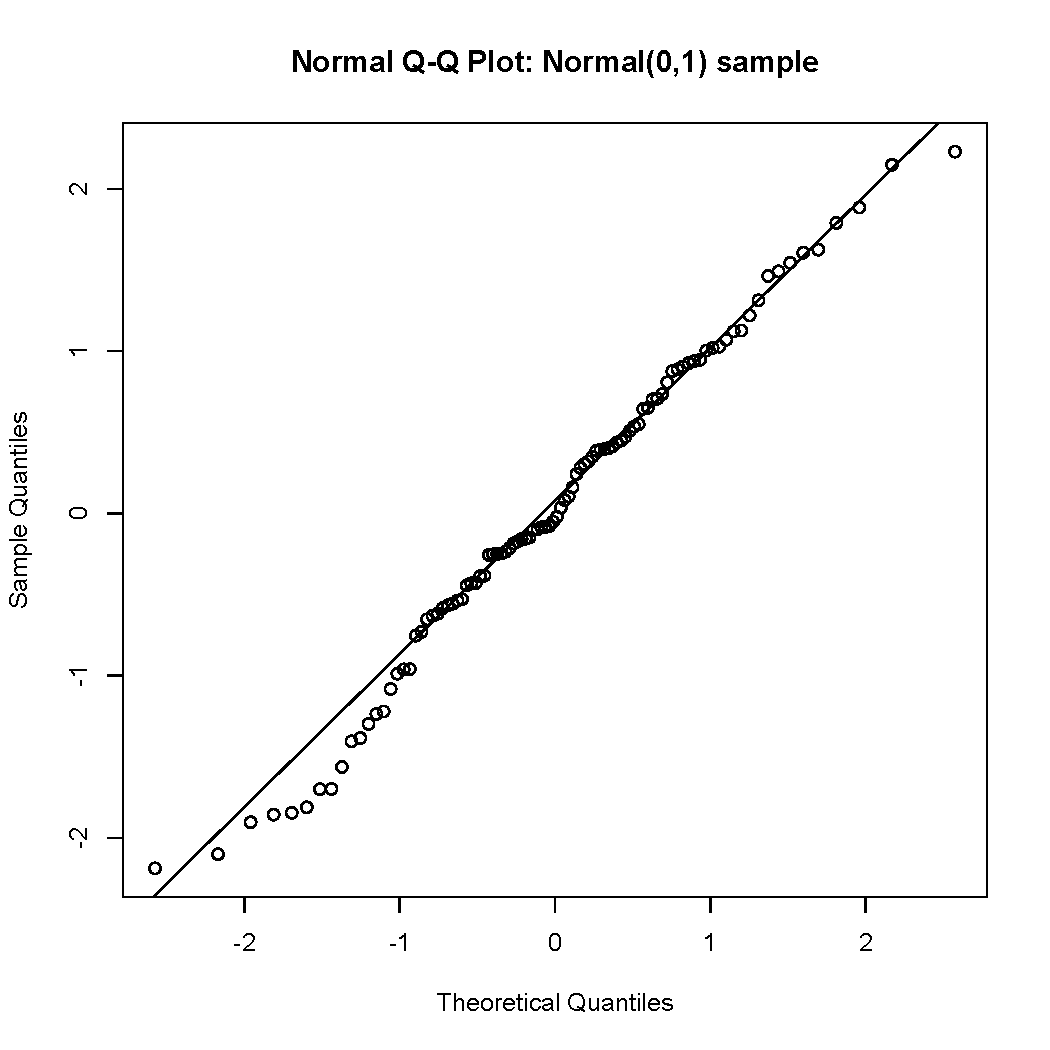
\includegraphics{nqqplot-normal}}
%\end{minipage}
%\hfill
%\begin{minipage}{0.45\linewidth}
%\resizebox{\linewidth}{!}{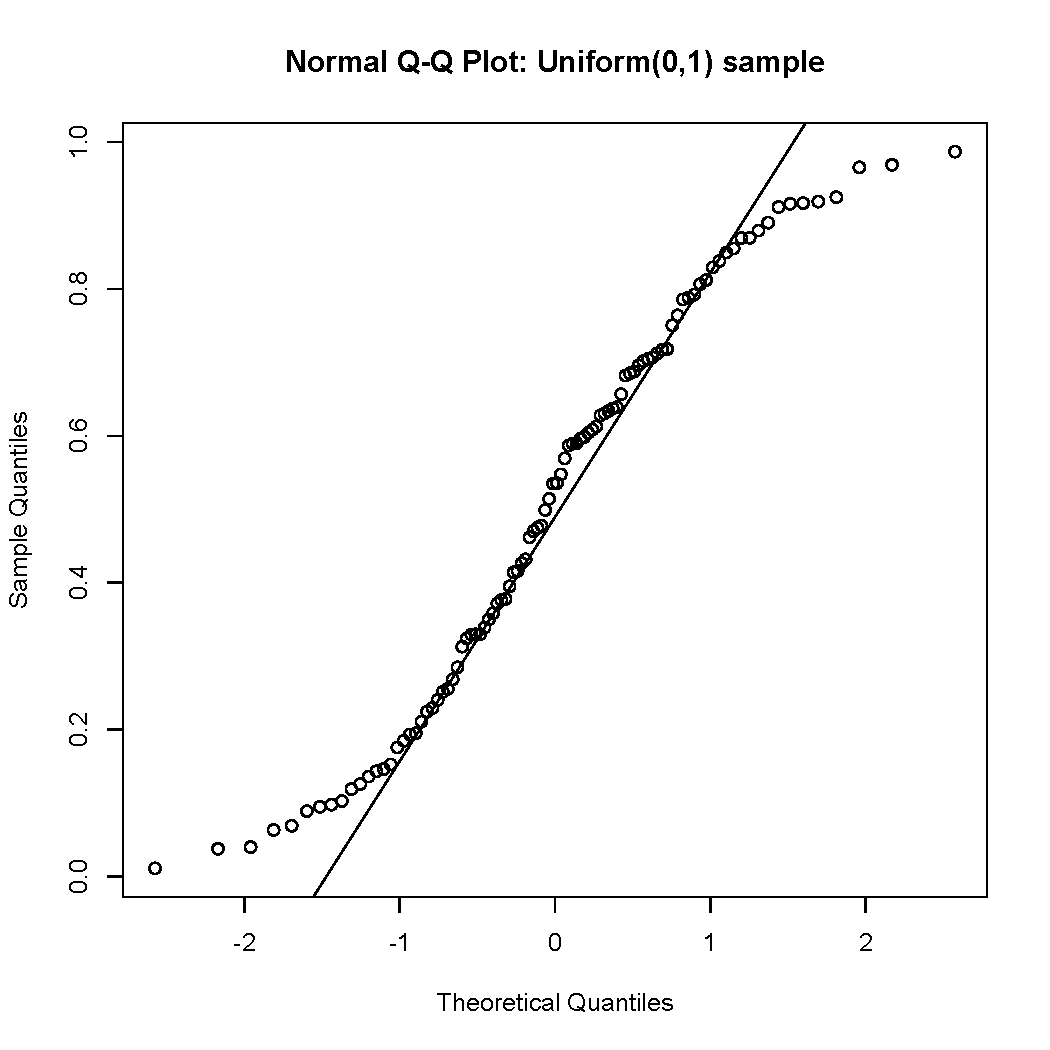
\includegraphics{nqqplot-uniform}}
%\end{minipage}
%\end{minipage}
\begin{figure}[ht]
\centering
\begin{tabular}{cc}
	\begin{subfigure}{0.45\textwidth}
	\resizebox{\linewidth}{!}{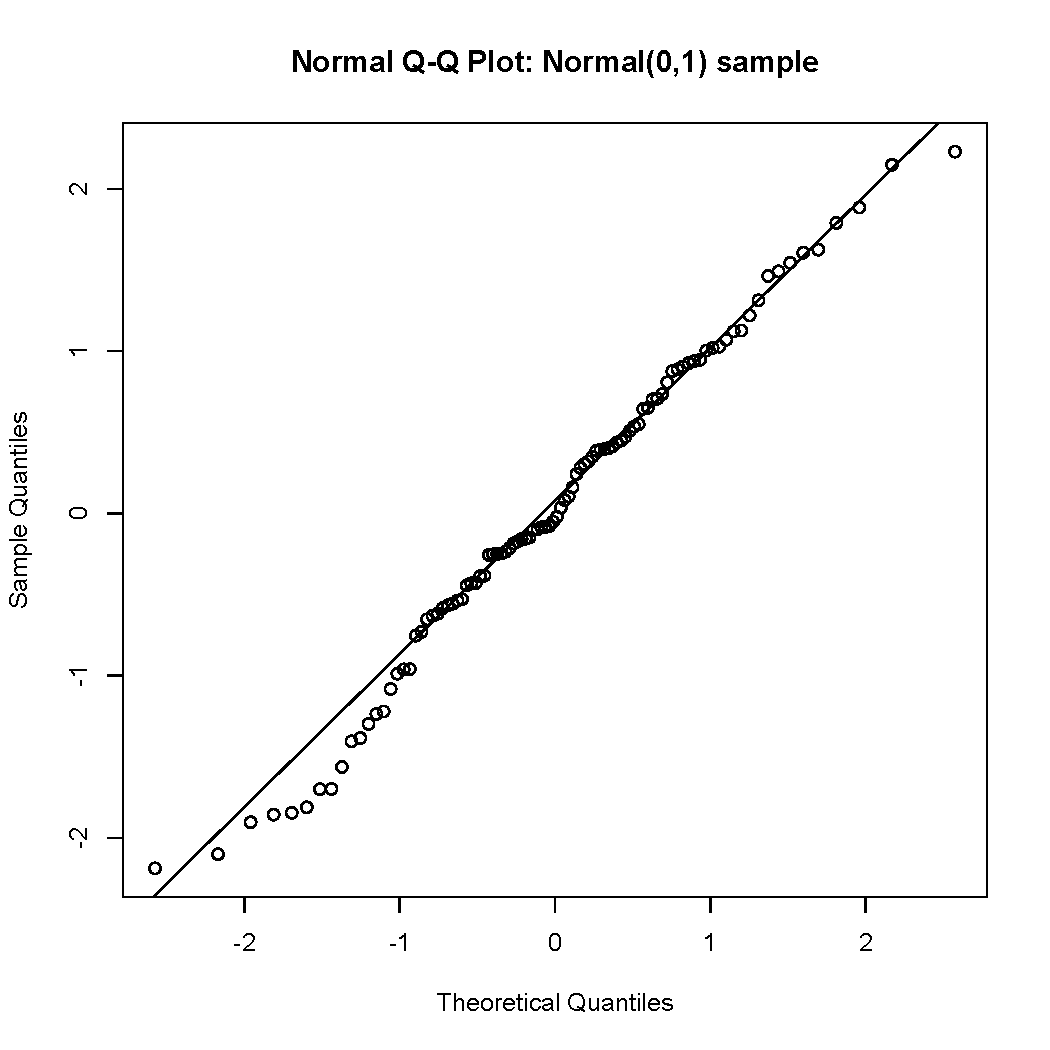
\includegraphics{nqqplot-normal}}
	\end{subfigure}
&
	\begin{subfigure}{0.45\textwidth}
	\resizebox{\linewidth}{!}{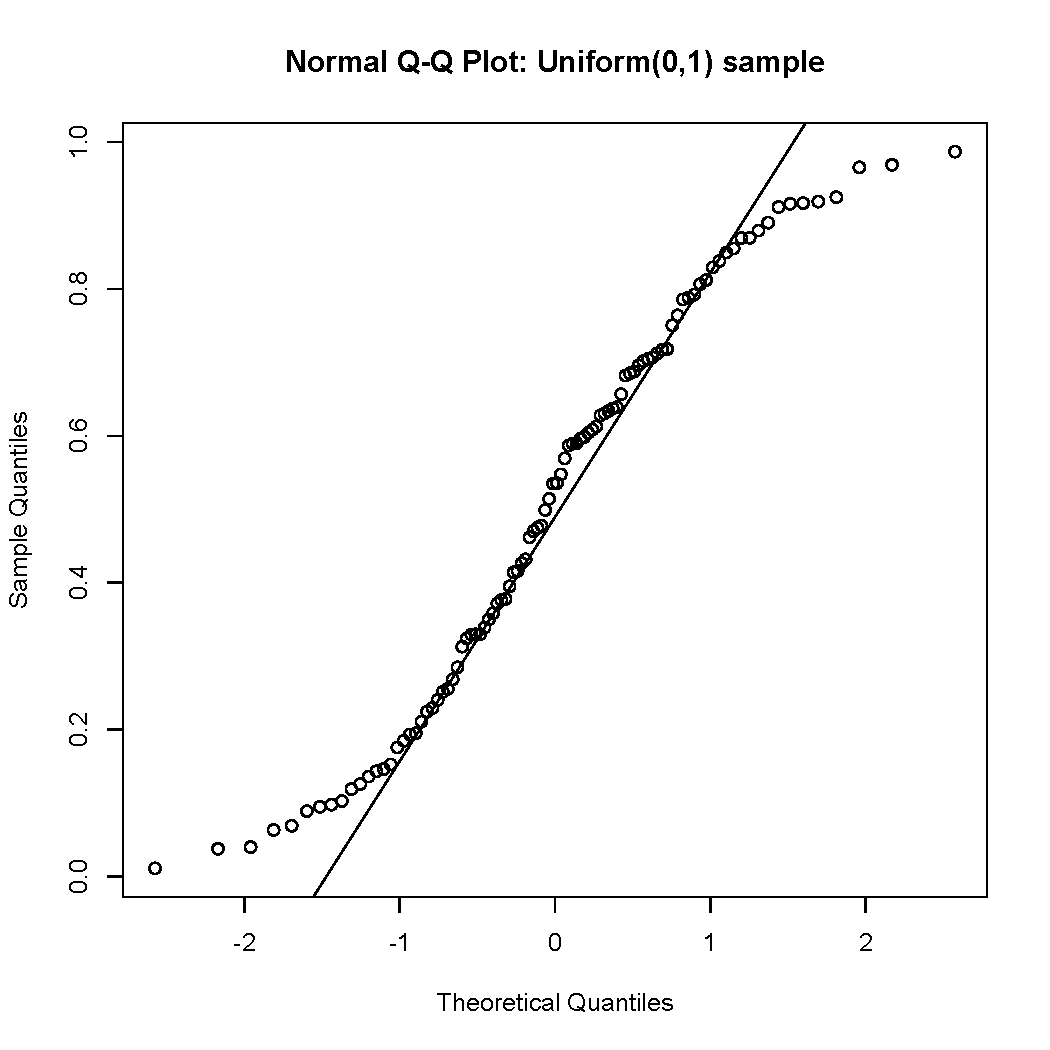
\includegraphics{nqqplot-uniform}}
	\end{subfigure}
\end{tabular}
\caption{Q-Q plots for testing normality.\label{fig:qq}}
\end{figure}

\end{example} 

% exercise (symmetric distributions)
\begin{exercise}
\begin{questions}
\question
Let $X$ be a random variable, let $F_X$ be its CDF and suppose that its distribution is symmetric about $a$.  Using the fact that $X-a$ and $-(X-a)$ have the same distribution, show that any location functional satisfies $T(F_X)=a$. 
\begin{answer}
Because $T$ is a location functional,
\[
T(F_{X-a}) = T(F_X)-a \qquad\text{and}\qquad T(F_{-(X-a)}) = -T(F_X)+a.
\]
Because $X-a$ and $-(X-a)$ have the same distribution, these are equal so $T(F_X)=a$, as required.
\end{answer}

\question %median and IQR
\begin{parts}
\part % median
Show that the median is a location functional.
\begin{answer}
Let $Y=a+bX$. Then
\[
F_{a+bX}(y) = \begin{cases}
	F_X\left(\frac{y-a}{b}\right)		& \text{ if $b>0$,} \\
	1 - F_X\left(\frac{y-a}{b}\right)	& \text{ if $b<0$.} 
\end{cases}
\]
Let $T(F_X)=F_X^{-1}(1/2)$ be the median functional. Then $F_X\big[T(F_X)\big] = 1/2$ so for $b>0$, 
\[
F_{a+bX}\big[a+bT(F_X)\big] = F_X\left[\frac{a+bT(F_X) - a}{b}\right] = F_X\big[T(F_X)\big] = 1/2,
\]
and for $b<0$, 
\[
F_{a+bX}\big[a+bT(F_X)\big] = 1 - F_X\left[\frac{a+bT(F_X) - a}{b}\right] = 1 - F_X\big[T(F_X)\big] = 1 - 1/2 = 1/2.
\]
In either case we have 
\[
T(F_{a+bX}) = F_{a+bX}^{-1}(1/2) = a+bT(F_X),
\]
so the median is a location functional, as required.
\end{answer}

\part % IQR
Show that the inter-quartile range is a scale functional.
\begin{answer}
Let $L(F_X) = F_X^{-1}(1/4)$ and $U(F_X)=F_X^{-1}(3/4)$ be the lower-quartile and upper-quartile functionals respectively. Then
\[
F_X\big[L(F_X)\big] = 1/4 \quad\text{and}\quad F_X\big[U(F_X)\big] = 3/4.
\]
For $b>0$, 
\begin{align*}
F_{a+bX}\big[a+bL(F_X)\big]
	& = F_X\left[\frac{a+bL(F_X) - a}{b}\right] = F_X\big[L(F_X)\big] = 1/4,\\
F_{a+bX}\big[a+bU(F_X)\big]
	& = F_X\left[\frac{a+bU(F_X) - a}{b}\right] = F_X\big[U(F_X)\big] = 3/4,\\
\end{align*}
Thus $L(F_{a+bX}) = F_{a+bX}^{-1}(1/4) = a+bL(F_X)$ and $U(F_{a+bX}) = F_{a+bX}^{-1}(3/4) = a+bU(F_X)$.

\bigskip
The inter-quartile range functional is $T(F_X)=U(F_X)-L(F_X)$, so
\[
T(F_{a+bX}) 
	= F_{a+bX}^{-1}(3/4) - F_{a+bX}^{-1}(1/4) 
	= \big[a+bU(F_X)\big] - \big[a + bL(F_X)\big]
	= b\big[U(F_X)-L(F_X)\big]
	= bT(F_X).
\]
Thus the inter-quartile range is a scale functional, as required.
\end{answer}
\end{parts}
\end{questions}
\end{exercise}



% !TEX root = main.tex

%-------------------------------------------------
\section{One-sample tests}\label{sec:np_one_sample_tests}

%-------------------------------------------------
\subsection{The sign test}\label{sec:signtest}

Let $X$ be a continuous random variable with an unknown median $\eta$. The sign test is a non-parametric method for testing hypotheses about $\eta$.

%%-----------------------------
%\subsection{The median}
%The non-parametric methods we consider are based on the \emph{median} of an unknown distribution.
%
%\begin{definition}
%A \emph{median} of a random variable $X$ is a real number $\eta$ satisfying
%\[
%\prob(X\leq\eta)\,\geq\frac{1}{2} \quad\text{and}\quad \prob(X\geq\eta)\,\geq\frac{1}{2}.
%\]
%If $X$ is a continuous random variable, its median is uniquely defined,
%\[
%\prob(X\leq\eta) = \prob(X\geq\eta) = \frac{1}{2}.
%\]
%\end{definition}
%
%\begin{example}
%Consider the random sample $\{1, 2, 2, 2, 3, 14\}$.
%\bit
%\it The sample median is $\hat{\eta} = 2$; the sample mean is $\hat{\mu}  = 4$.
%\eit
%In this case, $\hat{\eta}$ provides a better indicator of centrality than $\hat{\mu}$.
%\end{example}

%-----------------------------
\subsubsection{The test statistic}

Let $X_1,X_2,\ldots,X_n$ be a random sample from the distribution of $X$ and consider the null hypothesis $H_0:\eta=\eta_0$ against a suitable alternative. If $H_0$ is correct then approximately half of the observations should be smaller than $\eta_0$ and approximately half should be larger than $\eta_0$.

\begin{definition}
The sign test statistic $S^{+}_n$ is the number of observations larger than $\eta_0$: 
\[
S^{+}_n = \sum_{i=1}^n Z_i \quad\text{where}\quad Z_i=I(X_i>\eta_0).
\]
\end{definition}

We also define the complementary statistic $S^{-}_n = \displaystyle\sum_{i=1}^n (1-Z_i)$ which is the number of observations smaller than $\eta_0$. Note that $S^{+}_n + S^{-}_n = n$.

\bigskip
Because the observations are independent, the distribution of our test statistic under $H_0$ is
\[
S^{+}_n\sim\text{Binomial}(n,0.5).
\]
\bit
\it Small values of $S^{+}_n$ support the alternative $H_1:\eta < \eta_0$.
\it Large values of $S^{+}_n$ support the alternative $H_1:\eta > \eta_0$.
\eit

% example: sign test (one sample)
\begin{example}
The following are measurements of the breaking strength of a certain kind of two-inch cotton ribbon.
\[\begin{array}{cccccccccc}
163 & 165 & 158 & 189 & 161 & 171 & 158 & 151 & 169 & 162 \\
163 & 139 & 172 & 165 & 148 & 166 & 172 & 163 & 187 & 173 \\
\end{array}\]
Conduct a sign test to decide between $H_0:\eta=160$ and $H_1:\eta>160$ at significance level $\alpha=0.05$. 
\end{example}

\begin{solution}
First we must assume that the distribution of the breaking strength is continuous.
\small
\[\begin{array}{cccccccccc} \hline
163 & 165 & 160 & 189 & 161 & 171 & 158 & 151 & 169 & 162 \\
+ & + & - & + & + & + & - & - & + & + \\ \hline
163 & 139 & 172 & 165 & 148 & 166 & 172 & 163 & 187 & 173 \\
+ & - & + & + & - & + & + & + & + & + \\ \hline
\end{array}\]
\normalsize
\bit
\it We have $n=20$ signs: under the null hypothesis, $S^{+}_n\sim\text{Binomial}(20,0.5)$.
\it The observed value of the test statistic $s^{+}_n=15$. 
\it From tables we find that $\prob_{H_0}(S^{+}_n\geq 15) = 1 - 0.9793 = 0.0207$ approx. 
\it Thus we reject $H_0$ at significance level $\alpha=0.05$.
\eit
\end{solution}

% example: sign test (paired samples)
\begin{example}[Sign test for paired samples]
To evaluate a new traffic-control system, the number of accidents that occurred at 12 dangerous junctions were recorded during the four weeks prior to the installation of the new system, and for the four weeks after its installation. The following data were obtained.
\small
\[\begin{array}{|l|rrrrrrrrrrrr|} \hline
\text{Junction}	& \phantom{1}1 & \phantom{1}2 & \phantom{1}3 & \phantom{1}4 & \phantom{1}5 & \phantom{1}6 & \phantom{1}7 & \phantom{1}8 & \phantom{1}9 & 10 & 11 & 12 \\ \hline
\text{Before}	& 3 & 5 & 2 & 3 & 3 & 3 & 0 & 4 & 1 &  6 &  4 &  1 \\
\text{After}	& 1 & 2 & 2 & 2 & 2 & 0 & 2 & 3 & 3 &  4 &  1 &  0 \\ \hline
\end{array}\]
\normalsize
Use a sign test to evaluate the claim that the new system is more effective than the old system.
\end{example}

\begin{solution}
Let $\eta_1$ and $\eta_2$ denote the median number of accidents before and after the new system was installed, respectively. We test $H_0:\eta_1=\eta_2$ against $H_1:\eta_1 > \eta_2$.
\[\begin{array}{|l|rrrrrrrrrrrr|} \hline
\text{Junction}	& \phantom{1}1 & \phantom{1}2 & \phantom{1}3 & \phantom{1}4 & \phantom{1}5 & \phantom{1}6 & \phantom{1}7 & \phantom{1}8 & \phantom{1}9 & 10 & 11 & 12 \\ \hline
%\text{Before}		& 3 & 5 & 2 & 3 & 3 & 3 & 0 & 4 & 1 &  6 &  4 &  1 \\
%\text{After}		& 1 & 2 & 2 & 2 & 2 & 0 & 2 & 3 & 3 &  4 &  1 &  0 \\ \hline
\text{Difference}	& + & + & 0 & + & + & + & - & + & - &  + &  + &  + \\ \hline
\end{array}\]

\bit
\it We have $n=11$ observations (one discarded) so $S^{+}_n\sim\text{Binomial}(11,\theta)$ under $H_0$.
\it The value of the test statistic is $s^{+}_n = 9$.
\it Under $H_0:\theta=0.5$, from tables we obtain $\prob_{0.5}(S^{+}_n\geq 9) = 1 - 0.9673 = 0.0327$.
\it At $\alpha=0.05$ we reject $H_0$ and conclude that the system has indeed reduced the number of accidents.
\it At $\alpha=0.01$ we retain $H_0$ and conclude that there is insufficient evidence to support the claim.
\eit
\end{solution}

%-----------------------------
\subsubsection{Normal approximation}

By the central limit theorem, if $X\sim\text{Binomial}(n,\theta)$ then for large $n$,
\[
X\sim N\big(n\theta,n\theta(1-\theta)\big) \text{\quad approx.}
\]
If $H_0:\theta=0.5$ is correct, the distribution of the test statistic is $S^{+}_n\sim N(n/2,n/4)$ approx.

% continuity correction
\begin{definition}[The continuity correction]
Let $X$ be a discrete random variable, taking values in the set $\{0,\pm 1,\pm 2,\ldots\}$. If the distribution of a continuous random variable $Y$ is taken as an approximation of the distribution of $X$, we set
\[
\prob(X=k) = \prob\left(k - \frac{1}{2} < Y < k + \frac{1}{2}\right).
\] 
\end{definition}
This means that 
\bit
\it $\prob(X < k) = \prob(Y\leq k-1/2)$ and $\prob(X\leq k) = \prob(Y\leq k+1/2)$,
\it $\prob(X\geq k) = \prob(Y\geq k-1/2)$ and $\prob(X > k) = \prob(Y\geq k+1/2)$
\eit

% example: sign test (large sample)
\begin{example}[Sign test for large samples]
The following data are the amounts of sulphur oxide (in tonnes) emitted by a large industrial plant over a period of 40 days.
\[\begin{array}{cccccccccc}
17 & 15 & 20 & 29 & 19 & 18 & 22 & 25 & 27 &  9 \\
24 & 20 & 17 &  6 & 24 & 14 & 15 & 23 & 24 & 26 \\
19 & 23 & 28 & 19 & 16 & 22 & 24 & 17 & 20 & 13 \\
19 & 10 & 23 & 18 & 31 & 13 & 20 & 17 & 24 & 14
\end{array}\]
Construct a sign test of size $\alpha=0.01$ to evaluate $H_0:\eta=21.5$ against $H_1:\eta<21.5$.
\end{example}

\begin{solution}
Assume that sulphur oxide emissions per day has a continuous distribution. The sign test statistic is
\[
S^{+}_n = \sum_{i=1}^n I(X_i>21.5).
\]
and because the sample is relatively large, $S^{+}_n\sim N(n/2,n/4)$ approx.

\bigskip
Using the continuity correction (for a lower-tailed test), we have the test statistic
\[
Z = \displaystyle\frac{(S^{+}_n+1/2)-n/2}{\sqrt{n/4}} \sim N(0,1) \text{ approx.}
\]
Here, we have $n=40$ and $s^{+}_n=16$ (the number values exceeding $\mu_0 = 21.5$), so the value of the test statistic is
\[
z = \frac{16.5 - 20}{\sqrt{10}} = -1.1068.
\]
From tables, the (lower-tail) critical value of $N(0,1)$ at $\alpha=0.01$ is $z_c = \Phi^{-1}(0.01) = -2.33$ approx. Thus we retain $H_0$ and conclude that the median amount of sulphur oxide emitted by the plant is not less than $21.5$ tons per day.
\end{solution}

\begin{exercise}
\begin{questions}

\question % flies
The biting rate of a particular species of fly was investigated. The biting rate is defined as the number of flies biting a volunteer during $15$ minutes of exposure. The species is known to have a median biting rate of $5$ bites per $15$ minutes. It is hypothesized that the median biting range is higher in bright, sunny weather. To test the hypothesis, a total of $122$ volunteers were exposed to flies on a sunny day, of which $95$ experienced biting rates greater than $5$.
State the null and alternative hypotheses for the test, and state your conclusion for $\alpha = 0.01$.
\begin{answer}
Let $\eta$ deonte the (true) median biting rate. 
\par
The hypothesis test is $H_0:\eta=5$ against, $H_1:\eta>5$.
\par
The test statistic is $S_n^{+} = 95$ where $n=122$. 

\bigskip
Under the null hypothesis, $\prob(S_{122}^{+}\geq 95) = \prob\big[\text{Binomial}(122,0.5) \geq 95\big]$.

\bigskip
Since $n$ is large, we use the normal approximation: under the null hypothesis,
\[
Z = \frac{(S_n^{+}-1/2) - n/2}{\sqrt{n/4}} \sim N (0,1) \quad\text{approx.}
\]
In this case, the test statistic is
\[
z = \frac{94.5 - 61}{\sqrt{30.5}} = 6.0659.
\]
An approximate $p$-value is $\prob(Z>6.6059) < 0.001$, so we reject $H_0$ at $\alpha=0.01$.
\end{answer}

\question % sign-test v z-test
Let $X\sim N (\mu,1)$ where $\mu$ is unknown and suppose we wish to test the simple null hypothesis $H_0:\mu=0$ against the simple alternative $H_1:\mu=0.5$. A random sample of 9 observations is taken from the distribution of $X$ and the number $S^{+}$ of positive values is counted.
\ben
\it % << (i)
A sign test rejects the null hypothesis if $S^{+}$ exceeds $6$. Find the size and power of the test.
\it % << (ii)
Construct a test based on the sample mean of the observations which has the same significance level as the sign test described above. Find the power of the test, and explain why this is higher than the power of the sign test.
\een

\begin{answer}
\ben
\it % << (i)
Under the null hypothesis, $S^{+}\sim\text{Binomial}(9, 0.5)$. The size of the test is
\[
\alpha = \prob_{\mu_0}(S^{+}>6) = \prob\big(\text{Binomial}(9,0.5)>6\big) \approx 0.0898 \text{ (from tables)}.
\]
Under $H_1:\mu=0.5$ we have $X\sim N(0.5,1)$, so the probability that an observataion takes a positive value under $H_1$ is
\[
\prob_{\mu_1}(X > 0) 
	= \prob\big(X > 0 \text{ where } X\sim N(0.5,1)\big) 
	= \prob\big(Z > -0.5 \text{ where } Z\sim N(0,1)\big) 
	\approx 0.69146 \quad\text{(from tables).}
\]
The power of the test to detect the alternative $H_1:\mu=0.5$ is therefore
\[
\gamma(0.5) = \prob_{\mu_1}(S^{+}>6) = \prob\big[\text{Binomial}(9,0.6915) > 6\big] = \prob\big[\text{Binomial}(9,0.0.3085) < 3\big] 
\]
where the second equality follows by the fact that 
\[
\prob\big[\text{Binomial}(n,p) > k\big] = \prob\big[\text{Binomial}(n,1-p) < n-k\big].
\]
From tables, we find that 
\[
\prob[\text{Binomial}(9,0.30)\leq 2\big] \approx 0.4628  \quad\text{and}\quad \prob[\text{Binomial}(9,0.35)\leq 2\big] \approx 0.3373.
\]
To find the required probability, we interpolate between these values:
\begin{align*}
\prob\big[\text{Binomial}(9,0.3085)\leq 2\big]
	& \approx \prob\big[\text{Binomial}(9,0.30)\leq 2\big] \\
	& \qquad + \left(\frac{0.3085 - 0.30}{0.35 - 0.30}\right)\left(\prob\big[\text{Bino}(9,0.35)\leq 2\big]-\prob\big[\text{Bino}(9,0.30)\leq 2\big]\right) \\
	& = 0.4628 - (0.1708\times 0.1255) \\
	& = 0.4414.
\end{align*}	
Alternatively, we can use the normal approximation: if $Y\sim \text{Binomial}(9,0.6915)$ then $\expe(Y) = 6.2231$ and $\var(Y) = 1.9201$. Using the continuity correction,
\[
\prob\big[\text{Binomial}(9,0.6915) > 6\big]
	\approx \prob\left[ N (0,1) > \frac{6.5-6.2231}{\sqrt{1.9201}}\right]
	= \prob\big(N(0,1)> 0.1998\big) 
%	= 1 - 0.5793 
	\approx 0.4207.
\]	
\item % (ii)
Let $\bar{X}$ denote the sample mean, and consider the $z$-test, where $H_0:\mu=0$ is rejected in favour of $H_1:\mu=0.5$ if $\bar{X} > c$, with $c$ chosen to give the required significance level. Here we require $\alpha = 0.0898$, so we need
\[
\prob_{\mu_0}(\bar{X} > c) = 0.0898.
\]
Under $H_0$ we have $X_i\sim N (0,1)$, so $\expe(\bar{X})=0$ and $\var(\bar{X})=1/9$. Thus $\bar{X}\sim N (0,1/9)$, so the critical value $c$ satisfies
\[
\prob\left( N (0,1) > \frac{c}{\sqrt{1/9}}\right) = 0.0898,
\]
i.e.\ $1-\Phi(3c) = 0.0898$, or $\Phi(3c) = 0.9102$. From tables, $\Phi(1.34076) = 0.91$ and $\Phi(1.40507)= 0.92$. Interpolating linearly between these values gives
\[
3c = 1.34076 + 0.02(1.40507 - 1.34076) = 1.342,
\]
so $c\approx 0.447$. The statistical power is 
\begin{align*}
\gamma(0.5) = \prob_{H_1}(\bar{X} > 0.447) 
	& = \prob\big(N(0.5,1/9) > 0.447\big) \\
	& = \prob\big(N(0,1) > 3(0.447 - 0.5)\big) \\
	& = \prob\big(N(0,1) > -0.159)\big) \\
	& \approx 0.564 \quad\text{(from tables).}
\end{align*}
This is higher than the power of the sign test (which is approximately $0.43$), because the $z$-test takes account of the magnitude of the observations, as well as their signs. If the data really do come from a normal distribution, the $z$-test is more powerful than the sign test for detecting $H_1:\mu=0.5$ against $H_0:\mu=0$.
\een
\end{answer}
\end{questions}
\end{exercise}


%-------------------------------------------------
\subsection{The Wilcoxon signed-rank test}\label{sec:wsr_test}

The Wilcoxon signed rank test is an extension of the sign test.
\bit
\it The sign test counts the \emph{number} of observations which are larger than some fixed value.
\it The WSR test also considers the \emph{relative size} of these observations.
\eit

%-----------------------------
%\subsubsection{Ranks}

\begin{definition}
For a random sample $X_1,\ldots,X_n$, the \emph{rank} of observation $X_i$ is its position in the sequence of observations sorted in ascending order:
\[
R(X_i) = \sum_{j=1}^n I(X_j \leq X_i)
\]
\end{definition}

Note that the sum of the ranks is always equal to the sum of the first $n$ positive integers:
\[
\displaystyle \sum_{i=1}^n R(X_i) = \sum_{i=1}^n i = \frac{1}{2}n(n+1).
\]

\begin{remark}[Ties]
If two or more observations have the same value, they are said to be \emph{tied}. If the distribution is continuous, ties occur with probability zero. Ties often occur in practical applications however, due to the limited precision of measurements. To deal with ties, the usual approach is to assign an \emph{average rank} to each of the tied observations. For example, if there are $m-1$ observations strictly smaller than $X_i=X_j$, we set
\[
R(X_i) = R(X_j) = \frac{m+(m+1)}{2} = m+\frac{1}{2}.
\]
\end{remark}

%-----------------------------
\subsubsection{The test statistic}

Let $X$ be a continuous random variable whose distribution is \emph{symmetric} and whose median $\eta$ is unknown, and let $X_1,X_2,\ldots,X_n$ be a random sample from the distribution of $X$. 
Without loss of generality, we consider the null hypothesis $H_0:\eta=0$:
\bit
\it for a single sample $X_1,X_2,\ldots,X_n$, the null hypothesis $H_0:\eta=\eta_0$ reduces to $H_0:\eta=0$ by looking at the differences $D_i = X_i - \eta_0$;
\it For paired samples $X_1,X_2,\ldots,X_n$ and $Y_1,Y_2,\ldots,Y_n$, the null hypothesis $H_0:\eta_1=\eta_2$ reduces to $H_0:\eta=0$ by looking at the differences $D_i = X_i - Y_i$.
\eit

% definition: wsr statistic
\begin{definition}
For the null hypothesis $H_0:\eta=0$, the \emph{Wilcoxon signed rank} (WSR) statistic is 
\[
W^{+}_n = \sum_{i=1}^n R_i Z_i \quad\text{where}\quad R_i = \sum_{j=1}^n I(|X_j|\leq |X_i|) \quad\text{and}\quad Z_i=I(X_i>0).
\]
\end{definition}
\bit
\it $R_i$ is the rank of $|X_i|$ in the sample of absolute values $|X_1|,|X_2|,\ldots,|X_n|$;
\it $Z_i=1$ if $X_i>0$, otherwise $Z_i=0$.
\eit

We also define the complementary statistic $W^{-}_n = \displaystyle\sum_{i=1}^n R_i(1-Z_i)$. Note that
\[
W^{+}_n + W^{-}_n = \sum_{i=1}^n R_i = \sum_{i=1}^n i = \frac{1}{2}n(n+1).
\]

%% test procedure
%The WSR test procedure is as follows:
%\ben
%\it Compute the differences $D_i = X_i - \eta_0$ (single sample) or $D_i=X_i-X'_i$ (matched pairs).
%\it Compute absolute differences $|D_i|$ and record the sign of $D_i$.
%\it Compute the ranks $R_i$ of the absolute differences $|D_i|$.
%\it Compute the the sum of the ranks of those $|D_i|$ having positive sign. 
%\een
%The final step yields the test statistic $W^{+}_n$.

% example
\begin{example}
A study of the effects of smoking by mothers on the birthweight of their children involved 12 pairs of mothers. The pairs of mothers were selected so that they were as similar as possible, except that one mother of each pair was a smoker and the other was not. The birthweights (in kilograms) of the babies were as follows.
\small
\[\begin{array}{l|cccccccccccc} \hline
\text{Pair}			& 1      &  2     & 3      & 4      & 5      & 6      & 7      & 8      & 9      & 10     & 11     & 12 		\\ \hline
\text{Non-smoker}	& 3.22   & 4.48   & 3.90   & 3.47   & 3.07   & 3.23   & 4.25   & 3.31   & 3.33   & 3.78   & 3.18   & 4.60  	\\ 
\text{Smoker}		& 3.00   & 4.27   & 3.95   & 3.32   & 2.51   & 2.77   & 4.02   & 3.41   & 3.39   & 3.88   & 3.18   & 4.37 	\\ \hline
\end{array}\]
\normalsize
Do these data support the claim that mothers who smoke tend to have babies with smaller birthweights than those who do not? 
\end{example}

\begin{solution}
The data are in matched pairs so we compute the differences $D_i=X_i-Y_i$, where $X_1,X_2,\ldots,X_n$ are the birthweights for non-smokers and $Y_1,Y_2,\ldots,Y_n$ are the corresponding birthweights for smokers. The test then becomes
\[
H_0:\eta = 0 \quad\text{against}\quad H_1:\eta > 0,
\]
where $\eta$ is the (true) median difference between birthweights for the non-smoking group and birthweights for the smoking group.

\small
\[\begin{array}{|c|cccccccccccc|} \hline
i			& 1      &  2     & 3      & 4      & 5      & 6      & 7      & 8      & 9      & 10     & 11     & 12   	\\ \hline
X_i			& 3.22   & 4.48   & 3.90   & 3.47   & 3.07   & 3.23   & 4.25   & 3.31   & 3.33   & 3.78   & 3.18   & 4.60 	\\ 
X'_i		& 3.00   & 4.27   & 3.95   & 3.32   & 2.51   & 2.77   & 4.02   & 3.41   & 3.39   & 3.88   & 3.18   & 4.37	\\ \hline
D_i			& 0.22   & 0.21   & -0.05  & 0.15   & 0.56   & 0.46   & 0.23   & -0.10  & -0.06  & -0.10  & 0.00  	& 0.23	\\
|D_i|		& 0.22   & 0.21   &  0.05  & 0.15   & 0.56   & 0.46   & 0.23   &  0.10  &  0.06  &  0.10  & 0.00  	& 0.23	\\ \hline
\text{sgn}(D_i)	& +      & +      & -      & +      & +      & +      & +      & -      & -      & -      &      	& +  	\\ 
%R(|D_i|)		& 8      & 7      & 2      & 6      & 12     & 11     & 9.5    &  4.5   &  3     &  4.5   & 0     	& 9.5  	\\ \hline
R(|D_i|)		& 7      & 6      & 1      & 5      & 11     & 10     & 8.5    &  3.5   &  2     &  3.5   &      	& 8.5  	\\ \hline
\end{array}\]
\vspace*{-2ex}\normalsize
\bit
\it The zero difference is discarded, leaving $n=11$ non-zero differences.
\it Ties are replaced by the average of the corresponding ranks.
\eit
From the data, $W^{+}_n = 56$ and $W^{-}_n = 10$. \Big[Check: $W^{+}_n + W^{-}_n = 66 = \frac{1}{2}n(n+1)$.\Big]
\bit
\it Large values of $W^{+}_n$ support the alternative hypothesis, $H_1:\eta > 0$. 
\it From tables, the upper-tail critical value of $W^{+}_n$ for $n=11$ at $\alpha=0.05$ is $w_c = 52$. 
\eit
Since $W^{+}_n > w_c$, we reject the null hypothesis and conclude that mothers who smoke tend to have babies with smaller birthweights than those who do not. 
\end{solution}


%-----------------------------
\subsubsection{Mean and variance of $W^{+}_n$}

% theorem: mean and variance of W+
\begin{theorem}
Let $X_1,X_2,\ldots,X_n$ be a random sample from a continuous distribution whose density function is symmetric about its mean. Under the null hypothesis $H_0:\eta=0$, 
\[
\expe(W^{+}_n) = \frac{n(n+1)}{4} \qquad\text{and}\qquad \var(W^{+}_n)	= \frac{n(n+1)(2n+1)}{24}.
\]
\end{theorem}

\begin{proof}
Recall that 
\[
W^{+}_n = \sum_{i=1}^n R_i Z_i \quad\text{where}\quad R_i = \sum_{j=1}^n I(|X_j|\leq |X_i|) \quad\text{and}\quad Z_i=I(X_i>0).
\]
%
%$W^{+}_n = \sum_{i=1}^n R_iZ_i$, where $R_i=R(|X_i|)$ and $Z_i = I(X_i > 0)$.
Under $H_0:\eta=0$ we have $Z_i\sim\text{Bernoulli}(1/2)$ and hence $\expe(Z_i)=1/2$ and $\var(Z_i)=1/4$. 

\begin{align*}
\expe(W^{+}_n) 
	& = \sum_{i=1}^n R_i\expe(Z_i) 
	= \frac{1}{2}\sum_{i=1}^n R_i
	= \frac{1}{2}\sum_{i=1}^n i
	= \frac{1}{4}n(n+1). \\
\var(W^{+}_n)
	& = \sum_{i=1}^n R_i^2 \var(Z_i) 
	= \frac{1}{4}\sum_{i=1}^n R_i^2
	= \frac{1}{4}\sum_{i=1}^n i^2
	= \frac{1}{24}n(n+1)(2n+1).
\end{align*}
\end{proof}

%\begin{remark}
%\bit
%\it
%In practice, the sum of the squares of the ranks is equal to the sum of the squares of the first $n$ natural numbers only if there are no ties and no zeros (i.e.\ observations that are exactly equal to $\eta_0$).
%\it A correction for ties is
%\[
%\var(W^{+}_n) = \frac{1}{24}n(n+1)(2n+1) - \frac{1}{48}\sum t(t^2-1)
%\]
%where $t$ is the number of tied observations (e.g.\ $t=2$ if there are two identical observations) and the summation is over the number of sets of tied observations.
%\eit
%\end{remark}

%-----------------------------
\subsubsection{Normal approximation}
$W^{+}_n$ is the sum of random variables and (although the random variables are not independent) it satisfies the central limit theorem. Under $H_0:\eta=0$, and provided $n$ is sufficiently large, the distribution of $W^{+}_n$ is 
\[
W^{+}_n \sim N\left(\frac{1}{4}n(n+1), \frac{1}{24}n(n+1)(2n+1)\right) \text{\quad approx.}
\]

The continuity correction should be applied when defining the test statistic.
\bit
\it Lower-talied test:
\[
Z = \frac{(W^{+}_n +\frac{1}{2})- \frac{1}{4}n(n+1)}{\sqrt{\frac{1}{24}n(n+1)(2n+1)}}\sim N(0,1) \quad\text{approx.}
\]
\it Upper-talied test:
\[
Z = \frac{(W^{+}_n -\frac{1}{2})- \frac{1}{4}n(n+1)}{\sqrt{\frac{1}{24}n(n+1)(2n+1)}}\sim N(0,1) \quad\text{approx.}
\]
\eit

%-----------------------------
\subsubsection{Exact distribution of $W^{+}_n$ under $H_0$}

The exact distribution of $W^{+}_n$ under $H_0$ can be obtained for small $n$ by a recurrence relation. The base case is $n=1$ (a single observation), for which $W^{+}_1\in\{0,1\}$ and under $H_0:\eta=0$,
\[
\prob(W^{+}_1 = 0) = \frac{1}{2} \quad\text{and}\quad \prob(W^{+}_1 = 1) = \frac{1}{2}.
\]
%
%
%\bit
%\it For $n = 2$, the set of ranks is $\{1,2\}$ so $W^{+}_2$ takes values in the set $\{0,1,2,3\}$. Under $H_0:\eta=0$, 
%%\small
%\[\begin{array}{|c|cccc|}\hline
%\text{Ranks}			& \{-1,-2\}	& \{+1,-2\}	& \{-1,+2\}	& \{+1,+2\}	\\ \hline
%k					& 0	& 1	& 2	& 3 \\ \hline
%\prob(W^{+}_2=k)		& 0.25		& 0.25		&  0.25		& 0.25 		\\ \hline
%\end{array}\]
%%\normalsize
%
%\it For $n=3$, the set of ranks is $\{1,2,3\}$, so $W^{+}_3$ takes values in the set $\{0,1,2,3,4,5,6\}$. Under $H_0:\eta=0$,
%%\small
%\[\begin{array}{|c|ccccccc|}\hline
%k				& 0		& 1		& 2		& 3 		& 4 		& 5 		& 6		\\ \hline
%\prob(W^{+}_3=k)	& 0.125	& 0.125	& 0.125	& 0.25	& 0.125	& 0.125	& 0.125	\\ \hline
%\end{array}\]
%%\normalsize
%\eit

% theorem
\begin{theorem}
Under $H_0:\eta=0$,
\[
\prob\big(W^{+}_{n+1}=k\big) = \frac{1}{2}\prob\big(W^{+}_n=k\big) + \frac{1}{2}\prob\big(W^{+}_n=k-(n+1)\big).
\]
%for $k=0,1,\ldots,\displaystyle\frac{1}{2}n(n+1)$ (and zero otherwise).
for $k=0,1,\ldots,\frac{1}{2}n(n+1)$, and zero otherwise.
\end{theorem}

\begin{proof}
\bit
\it Let $X_1,X_2,\ldots,X_n$ be a random sample from a continuous and symmetric distribution.
\it Let $R_i$ be the rank of $|X_i|$ among the absolute values $|X_1|,|X_2|,\ldots,|X_n|$:
\eit

Then $W^{+}_n$ can be written as
\[
W^{+}_n = \sum_{r=1}^n rU_r \qquad\text{where}\qquad U_{R_i} = \begin{cases} 1 & X_i > 0, \\ 0 & \text{otherwise.}\end{cases}
\]

\bit
\it $U_r$ indicates that the observation associated with rank $r$ has a positive sign.
\it Under the null hypothesis, $U_1,U_2,\ldots,U_n$ is a random sample from the $\text{Bernoulli}(1/2)$ distribution.
\eit

Let $G_n(t)$ denote the probability generating function of $W^{+}_n$:
\begin{align*}
G_n(t) 
	= \expe(t^{W^{+}_n})  
	= \expe(t^{\sum_{r=1}^n rU_r})
	& = \expe(t^{U_1}t^{2U_2}\cdots t^{nU_n}) \\
	& = \prod_{r=1}^n \expe(t^{rU_r}) \qquad\text{(by independence)} \\
	& = \prod_{r=1}^n \Big[t^0\,\prob(U_r=0) + t^r\,\prob(U_r=1)\Big] \\
	& = \prod_{r=1}^n \frac{1}{2}(1 + t^r). \\
\intertext{Hence,}
G_{n+1}(t) 
	& = \frac{1}{2}(1 + t^{n+1})G_n(t).
\end{align*}

By definition,
\begin{align*}
G_n(t)		= \sum_{k=0}^{\frac{1}{2}n(n+1)}\,\prob(W^{+}_n=k)t^k
\qquad\text{and}\qquad
G_{n+1}(t)	= \sum_{k=0}^{\frac{1}{2}(n+1)(n+2)}\,\prob(W^{+}_{n+1}=k)t^k.
\end{align*}

Thus,
\[
\sum_{k=0}^{\frac{1}{2}(n+1)(n+2)}\,\prob(W^{+}_{n+1}=k)t^k 
	= \frac{1}{2}(1+t^{n+1})\sum_{k=0}^{\frac{1}{2}n(n+1)}\,\prob(W^{+}_n=k)t^k,
\]

Comparing the coefficients of $t^k$ yields the required recurrence relation:
\[
\prob\big(W^{+}_{n+1}=k\big) = \frac{1}{2}\prob\big(W^{+}_n=k\big) + \frac{1}{2}\prob\big(W^{+}_n=k-(n+1)\big).
\]
This recurrence relation is used to compute the quantiles of $W^{+}_n$ listed in statistical tables.
\end{proof}


\begin{exercise}
\begin{questions}

\question
We wish to test the hypothesis that two treatments $A$ and $B$ are equivalent, against the alternative hypothesis that the responses to treatment $A$ tend to be larger than the responses to treatment $B$. We perform a paired difference experiment, and analyse the resulting data using the Wilcoxon signed rank test. The data is shown in the following table.
\[\begin{array}{|l|cccccccccc|}\hline
\text{Pair}	&  1 &  2 &  3 &  4 &  5 &  6 &  7 &  8 &  9 & 10 \\ \hline
$A$ 			& 54 & 60 & 98 & 43 & 82 & 77 & 74 & 29 & 63 & 80 \\
$B$ 			& 45 & 45 & 87 & 31 & 71 & 75 & 63 & 30 & 59 & 82 \\ \hline
\end{array}\]
State the null and alternative hypotheses for the test, and conduct the test at significance level $\alpha=0.05$.

\begin{answer}
\ben
\it % << (i)
Let $D_i=A_i-B_i$ denote the differences, and let $\eta$ denote the (true) median difference. We test the null hypothesis $H_0:\eta=0$ against the one-sided alternative $H_1:\eta>0$.
\it % << (ii)
The signed ranks are computed as follows:
\[\begin{array}{|l|cccccccccc|}\hline
\text{Pair}			&  1 &  2 &  3 &  4 &  5 &  6 &  7 &  8 &  9 & 10 \\ \hline
\text{Difference}	&  9 & 15 & 11 & 12 & 11 &  2 & 11 & -1 &  4 & -2 \\ \hline
\text{Signed Rank}	&  5 & 10 &  7 &  9 &  7 &2.5 &  7 & -1 &  4 & -2.5 \\ \hline
\end{array}\]
\bit
\it The Wilcoxon signed rank statistics are $W^{+} = 51.5$ and $W^{-}=3.5$. 
\it Check: $\frac{1}{2}n(n+1) = 55 = W^{+}+W^{-}$.
\it From tables, for a one-tailed test at $\alpha=0.05$ and $n=10$, the critical value is $w^{+}_c = 44$.
\it Thus we reject $H_0:\eta=0$ in favour of $H_1:\eta>0$, and conclude that responses to treatment $A$ tend to be larger than responses to treatment $B$.
\eit
\een
\end{answer}

\question
In a comparison of two populations $A$ and $B$, a paired difference experiment with $n=30$ pairs yields the Wilcoxon signed-rank statistic $w^{+}=354$.
\ben
\it Construct a test to determine whether or not population $A$ is located to the right of population $B$.
\it Conduct the test at $\alpha=0.05$.
\it Repeat part (2) using a normal approximation to the distribution of $W^{+}$.
\een

\begin{answer}
\ben
\it % << (i)
Let $\eta_A$ and $\eta_B$ denote the (true) medians of populations $A$ and $B$ respectively. To determine whether population $A$ is located to the right of population $B$, we test the null hypothesis $H_0:\eta_A=\eta_B$ against the alternative $H_1:\eta_A > \eta_B$. We could also define $\eta=\eta_A-\eta_B$ to be the difference between the two medians, in which case we would test $H_0:\eta=0$ agaianst $H_1:\eta>0$. 

\it % << (ii)
From tables, for a one-tailed test at $\alpha=0.05$ and $n=30$, the critical value is $w^{+}_c = 313$, so we reject $H_0$ in favour of $H_1$.

To compute an approximate $p$-value for the test, from tables (for $n=30$) we see that $w^{+}_c = 345$ at $\alpha=0.01$ and $w^{+}_c = 356$ at $\alpha=0.005$. Interpolating between these values, 
\[
\prob_{H_0}(W^{+}\geq 354) \approx 0.01 + \left(\frac{354-345}{356-345}\right)(0.005 - 0.01) = 0.0059.
\]

\it % << (ii)
The normal approximation is $\prob(W^{+}\geq w^{+}_c) \approx \prob(Z\geq z_c)$ where
\[
Z = \frac{(W^{+}-1/2) - \expe(W^{+})}{\sqrt{\var(W^{+})}} \sim N (0,1) \quad\text{approx.},
\]
Here, $\expe(W^{+})$ and $\var(W^{+})$ are respectively the mean and variance of $W^{+}$ under $H_0$. 
\par
In this case,
\[
\expe(W^{+}) = \frac{1}{4}n(n+1) = 232
\quad\text{and}\quad
\var(W^{+})  = \frac{1}{24}n(n+1)(2n+1) = 2363,
\]
so the test statistic is 
\[
z = \frac{353.5 - 232}{\sqrt{2363}} = 2.4994.
\]
\bit
\it At $\alpha=0.05$ we have $z_c = 1.645$, so we reject $H_0$. 
\it From tables, an approximate $p$-value for the test is $1-0.99379 = 0.0062$.
\eit
\een
\end{answer}

\question
To test whether or not a new diet actually results in weight loss, a researcher recruited nine subjects, measured their weight (in kilograms) before starting the diet, and then again after two months on the diet. The results are shown in the following table.
\[\begin{array}{|l|ccccccccc|} \hline
\text{Case}			&  1 &  2 &  3 &  4 &  5 &  6 &  7 &  8 &  9 \\ \hline
\text{Weight before }	& 55 & 50 & 54 & 43 & 62 & 61 & 56 & 48 & 53 \\
\text{Weight after }		& 47 & 40 & 52 & 43 & 51 & 62 & 50 & 47 & 56 \\ \hline
\end{array}\]

\begin{parts}
\part
Use a sign test with $\alpha=0.05$ to decide whether or not the diet results in weight loss.
\begin{answer}
Let $\eta$ denote the (true) median weight loss. 
\par
We evaluate $H_0:\eta = 0$ against the alternative $H_0:\eta > 0$.
\[\begin{array}{|l|ccccccccc|} \hline
\text{Case } (i)			&  1 &  2 &  3 &  4 &  5 &  6 &  7 &  8 &  9 \\ \hline
\text{Weight before }	& 55 & 50 & 54 & 43 & 62 & 61 & 56 & 48 & 53 \\
\text{Weight after }		& 47 & 40 & 52 & 43 & 51 & 62 & 50 & 47 & 56 \\ \hline
\text{Difference } (D_i)	&  8 & 10 &  2 &  0 & 11 & -1 &  6 &  1 & -3 \\ \hline
\text{Sign }				&  + &  + &  + &    &  + &  - &  + &  + &  - \\ \hline
%\text{Rank } (R_i)		&  6 &  7 &  3 &    &  8 &1.5 &  5 &1.5 &  4 \\ \hline
\end{array}\]
\bit
\it Exclude the zero difference, and take the sample size to be $n=8$.
\it $S_n^{+} = \sum_i I(D_i>0) = 6$.
\it $S_n^{-} = \sum_i I(D_i<0) = 2$. 
\it Check: $S_n^{+} + S_n^{-} = n$.
\eit
Under $H_0$, $S_n^{+}\sim\text{Binomial}(n,0.5)$. From tables,
\[
\prob_{H_0}(S_n^{+}\geq 6) = 1 - \prob_{H_0}(S_n^{+}\leq 5) = 1 - 0.8555 = 0.1445.
\]
At $\alpha=0.05$, we would decide to retain the null hypothesis $H_0:\eta=0$, and conclude that the diet results in no weight loss.
\end{answer}

\part
Repeat the analysis using the Wilcoxon signed rank test.
\begin{answer}
\[\begin{array}{|l|ccccccccc|} \hline
\text{Difference } (D_i)	&  8 & 10 &  2 &  0 & 11 & -1 &  6 &  1 & -3 \\ \hline
\text{Sign }				&  + &  + &  + &    &  + &  - &  + &  + &  - \\ \hline
\text{Rank } (R_i)		&  6 &  7 &  3 &    &  8 &1.5 &  5 &1.5 &  4 \\ \hline
\end{array}\]
\bit
\it $W^{+} = \sum_i R_i I(D_i>0) = 6 + 7 + 3 + 8 + 5 + 1.5 = 30.5$.
\it $W^{-} = \sum_i R_i I(D_i<0) = 1.5 + 4 = 5.5$.
\it Check: $W^{+} + W^{-} = \frac{1}{2}n(n+1)$.
\eit
From tables, critical values for an upper-tail test are
\bit
\it $w^{+}_c = 30$ at $\alpha=0.05$, and 
\it $w^{+}_c = 32$ at $\alpha=0.025$.
\eit
Thus at $\alpha=0.05$ we would reject the null hypothesis $H_0:\eta = 0$ in favour of the alternative $H_0:\eta > 0$, and conclude that the diet does indeed result in weight loss.
\end{answer}

\part
Briefly discuss the reasons why the tests lead to different conclusions.
\begin{answer}
The sign test takes no account of the fact that the average amount of weight lost by those whose weight decreased over the study period, is significantly greater than the average amount of weight gained by those whose weight increased over the study period. 
\end{answer}
\end{parts}

\end{questions}
\end{exercise}






% !TEX root = main.tex

\chapter{Bivariate analysis}\label{chap:bivariate}

% !TEX root = main.tex

%-------------------------------------------------
\section{Two-sample tests}\label{sec:two-sample-tests}

So far we have looked at one-sample tests, where hypotheses about an unknown parameter are tested based on a single sample $X_1,X_2,\ldots,X_n$ from the distribution in question. For paired samples $X_1,X_2,\ldots,X_n$ and $Y_1,Y_2,\ldots,Y_n$ we apply one-sample tests to the differences $D_i=X_i-Y_i$. We now turn our attention to the question of whether two \emph{independent} random samples are drawn from the same distribution.
\bit
\it \emph{Welch's t-test} is a parametric test to detect a difference between the means of two independent samples.
\it The \emph{Mann-Whitney test} is a non-parametric test to detect a difference between the medians of two independent samples.
\eit
%-----------------------------
\subsection{Welch's t-test}
Let $X\sim N(\mu_1,\sigma_1^2)$ and $Y\sim N(\mu_2,\sigma_2^2)$ be independent random variables, and suppose we with to test the null hypothesis $H_0:\mu_1=\mu_2$ against a suitable alternative. Let $X_1,X_2,\ldots,X_m$ be a random sample from the distribution of $X$ and let $Y_1,Y_2,\ldots,Y_n$ be a random sample from the distribution of $Y$. 

Using characteristic functions it can be shown that a linear combination of normal variables is a normal variable: if $X\sim N(\mu_1,\sigma_1^2)$ and $Y\sim N(\mu_2,\sigma^2_2)$ then
\[
aX+bY\sim N(a\mu_1+b\mu_2, a^2\sigma_1^2 + b^2\sigma_2^2).
\]
In particular,
\[
X-Y\sim N(\mu_1-\mu_2, \sigma_1^2 + \sigma_2^2).
\]
Because the samples are independent,
\[
\bar{X} - \bar{Y} \sim N\left(\mu_1-\mu_2, \frac{\sigma_1^2}{m} + \frac{\sigma_2^2}{n}\right).
\]

To estimate the variances $\sigma_1^2$ and $\sigma_2^2$ we use the sample variances of $X$ and $Y$:
%$S_1^2 = \displaystyle\frac{1}{m-1}\sum_{i=1}^m (X_i-\bar{X})^2$ and $S_2^2 = \displaystyle\frac{1}{n-1}\sum_{j=1}^n (Y_j-\bar{Y})^2$ 
\[
S_1^2 = \displaystyle\frac{1}{m-1}\sum_{i=1}^m (X_i-\bar{X})^2
\quad\text{and}\quad
S_2^2 = \displaystyle\frac{1}{n-1}\sum_{j=1}^n (Y_j-\bar{Y})^2.
\]
Our test statistic is
\[
T = \frac{(\bar{X}-\bar{Y})-(\mu_1-\mu_2)}{\sqrt{S_1^2/m + S_2^2/n}} %\sim t_{n-2} \quad\text{under $H_0:\mu_1=\mu_2$.} 
\]
\bit
\it Under $H_0:\mu_1=\mu_2$ we have that $T\sim t_{\nu}$ approximately, where
\[
\nu = \frac{(s_1^2/m+s_2^2/n)^2}{(s_1^2/m)^2(m-1) + (s_2^2/n)^2(n-1)} \qquad\text{(Welch-Satterthwaite equation).}
\]
%(Student's $t$-distribution with $n-2$ degrees of freedom).
\it An approximate $100(1-\alpha)\%$ large-sample confidence interval for the difference $\mu_1-\mu_2$ is given by
\[
(\bar{X}-\bar{Y}) \pm z_{\alpha/2}\sqrt{\frac{S_1^2}{m}+\frac{S_2^2}{n}}.
\]
\eit

%To test the null hypothesis $H_0:\mu_1=\mu_2$ we define the test statistic
%\[
%T = \frac{(\bar{X}-\bar{Y})-(\mu_1-\mu_2)}{\sqrt{S_1^2/m + S_2^2/n}} \sim t_{n-2} \quad\text{under $H_0:\mu_1=\mu_2$.} 
%\]

%For large samples, an approximate $100(1-\alpha)\%$ confidence interval for the difference $\mu_1-\mu_2$ is given by
%\[
%(\bar{X}-\bar{Y}) \pm z_{\alpha/2}\sqrt{\frac{S_1^2}{m}+\frac{S_2^2}{n}}
%\]

%-----------------------------
\subsubsection*{Equal variances}
Suppose that $X$ and $Y$ have equal variances: $X\sim N(\mu_1,\sigma^2)$ and $Y\sim N(\mu_2,\sigma^2)$ so that their distributions belong to the location model $\mathcal{M}=\{N(\mu,\sigma^2):\mu\in\R\}$. In this case we define the so-called \emph{pooled estimator} of variance,
\[
S_p^2 = \frac{(m-1)S_1^2 + (n-1)S_2^2}{m+n-2}.
\]
It is easy to show that $S_p^2$ is an unbiased estimator of $\sigma^2$, and that
%\[
%T = \frac{(\bar{X}-\bar{Y})-(\mu_1-\mu_2)}{S_p\sqrt{\frac{1}{m}+\frac{1}{n}}} \sim t_{m+n-2}. 
%\]
\[
T = \frac{(\bar{X}-\bar{Y})-(\mu_1-\mu_2)}{S_p\sqrt{1/m+1/n}} \sim t_{m+n-2} \quad\text{under $H_0:\mu_1=\mu_2$}. 
\]

\begin{example}
Let $X_1,X_2,\ldots,X_{10}$ be a random sample from the $N(\mu_1,\sigma^2)$ distribution, and let $Y_1,Y_2,\ldots,Y_7$ be an independent random sample from the $N(\mu_2,\sigma^2)$ distribution. Realisations of the samples yield the sample means $\bar{x}=4.2$ and $\bar{y}=3.4$ and the sample variances $s_1^2=49$ and $s_2^2=32$. 
\ben
\it Test the hypothesis $H_0:\mu_1=\mu_2$ against $H_1:\mu_1>\mu_2$.
\it Find a $90\%$ confidence interval for the difference $\mu_1-\mu_2$.
\een
\begin{solution}
\ben
\it With $m=10$ and $n=7$, the pooled estimator of variance is
\[
s_p^2 = \frac{(m-1)s_1^2 + (n-1)s_2^2}{m + n - 2} = \frac{(9\times 49) + (6\times 32)}{10 + 7 - 2} = 633/15 = 42.2
\]
The test statistic is 
\[
T = \frac{(\bar{X}-\bar{Y})-(\mu_1-\mu_2)}{S_p\sqrt{\frac{1}{m}+\frac{1}{n}}} \sim t_{m+n-2}\text{ under $H_0:\mu_1=\mu_2$.}
\]
The observed value of the test statistic is
\[
t = \frac{(\bar{x}-\bar{y})}{s_p\sqrt{1/m+1/n}} \frac{0.8}{\sqrt{4.2(1/10+1/7)}} = 0.7921 \text{ (approx.)}
\]
Under $H_0:\mu_1=\mu_2$, $T\sim t_{m+n-2}$. Upper-tail critical values are 1.341 (10\%) and 1.753 (5\%), so there is not enough evidence to reject the null hypothesis $H_0:\mu_1=\mu_2$. 
\it % ci
A $90\%$ confidence interval for $\mu_1-\mu_2$ is
\[
(\bar{x}-\bar{y}) \pm t_c s_p\sqrt{1/m+1/n} = (0.8\pm 1.753\times 6.4962\times\sqrt{1/10+1/7}) = (-4.81, 6.41).
\]
\een
\end{solution}
\end{example}

%-------------------------------------------------
\subsection{The Mann-Whitney test}\label{sec:mw_test}

%The \emph{Mann-Whitney test} is a non-parametric test to detect a difference between the medians of two independent samples.

%Let $X$ and $Y$ be two independent random variables having the same distribution, which is assumed to be continuous and symmetric, except that their medians $\eta_1$ and $\eta_2$ might be different. We test the null hypothesis $H_0:\eta_1 = \eta_2$ against a suitable alternative.

% definition: mw statistic
\begin{definition}
Let $X_1,X_2,\ldots,X_m$ be a random sample from a continuous and symmetric distribution with median $\eta_1$, and let $Y_1,Y_2,\ldots,Y_n$ be a random sample from a possibly shifted version the same distribution, with median $\eta_2$. To test the null hypothesis $H_0:\eta_1=\eta_2$ against a suitable alternative, the \emph{Mann-Whitney} test statistic is
\[
U_{m,n} = \sum_{i=1}^m \sum_{j=1}^n Z_{ij} 
\qquad\text{where}\qquad 
Z_{ij} = \begin{cases} 
	1 	& X_i < Y_j, \\
	0.5	& X_i = Y_j, \\
	0	& X_i > Y_j.
\end{cases}
\]
\end{definition}

We also define the complementary statistic 
\[
U'_{m,n} = \displaystyle\sum_{i=1}^m \sum_{j=1}^n (1-Z_{ij}).
\]
Note that $\min(U_{m,n})=0$, $\max(U_{m,n})=mn$, and
\[
U_{m,n} + U'_{m,n} = \sum_{i=1}^m\sum_{j=1}^n \big[Z_{ij} + (1-Z_{ij})\big] = \sum_{i=1}^m\sum_{j=1}^n 1 = mn,
\]

The direction of the alternative hypothesis determines how the test statistic should be used:
\par
\begin{tabular}{ll}
$\bullet$ $H_1:\eta_1 < \eta_2$:			& large values of $U$ support the alternative hypothesis. \\
$\bullet$ $H_1:\eta_1 > \eta_2$:			& small values of $U$ support the alternative hypothesis. \\
$\bullet$ $H_1:\eta_1 \neq \eta_2$:\qquad	& small and large values of $U$ support the alternative hypothesis.
\end{tabular}

% example
\begin{example}
Suppose we have the random sample $\{14,5,8\}$ from the distribution of $X$, and the random sample $\{7,12,18,11\}$ from the distribution of $Y$. Compute the Mann-Whitney test statistic for these data.
\end{example}
\begin{solution}
\[\begin{array}{|c|cccc|}\hline
X_i		& 14		&  5		&  8		& \\ \hline
Y_j		&  7		& 12		& 18		& 11 \\ \hline 
\end{array}\]
\bit 
\it $U$ is computed by counting the number of $X_i$ that are smaller than each $Y_j$.
\it $U'$ is computed by counting the number of $Y_j$ that are smaller than each $X_i$.
\eit
\begin{align*}
u 	& = 1 + 2 + 3 + 2 = 8 \\
u'	& = 3 + 0 + 1 = 4
\end{align*}
Check: $u+u' = 8 + 4 = 12 = mn$.
\end{solution}

% example
\begin{example}\label{ex:mannwhitney}
Two different models of car, with engines of a similar size, were compared for their fuel consumption. Five cars of each model were evaluated in independent tests. The observation made was the number of miles travelled using 10 litres of petrol. Use a suitable non-parametric test to assess the claim that Model~2 is more economical than Model~1.
\[\begin{array}{|l|ccccc|}\hline
\text{Model 1}	& 125.8	& 126.7	& 128.3	& 130.5	& 126.2 \\
\text{Model 2}	& 127.8 & 131.4	& 129.6	& 130.2	& 128.1 \\ \hline
\end{array}\]
\end{example}
\begin{solution}
The hypothesis test is $H_0:\eta_1=\eta_2$ against $H_1:\eta_1 < \eta_2$, where
\bit
\it $\eta_1$ is the median number of miles travelled by Model~1, and
\it $\eta_2$ is the median number of miless travelled by Model~2.
\eit
Only large values of $U$ support the alternative hypothesis. 
From tables ($m=5$, $n=5$), the critical value at significance level $\alpha=0.05$ is $u_c=21$. 
From the data,
\begin{align*}
u 		& = \sum_{i=1}^5\sum_{j=1}^5 Z_{ij} = 5 + 5 + 3 + 1 + 5 = 19. \\
u'		& = \sum_{i=1}^5\sum_{j=1}^5 (1-Z_{ij}) = 0 + 0 + 2 + 4 + 0 = 6.
\end{align*}
Check: $u + u' = mn = 25$. 
\par
Since the observed value $u=19$ is smaller than the critical value $u_c=21$, there is insufficient evidence to conclude that Model~2 is more economical than Model~1. 
\end{solution}

%-----------------------------
\subsubsection{Mean and variance of $U_{m,n}$}

\begin{theorem}
%Let $X_1,X_2,\ldots,X_m$ be a random sample from a continuous and symmetric distribution with median $\eta_1$, and let $Y_1,Y_2,\ldots,Y_n$ be a random sample from a possibly shifted version the same distribution, with median $\eta_2$. 
Under the null hypothesis $H_0:\eta_1=\eta_2$, 
\[
\expe(U_{m,n}) = \frac{mn}{2}
\text{\quad and\quad}
\var(U_{m,n}) = \frac{mn}{12}(m+n+1).
\]
\end{theorem}

\begin{proof}
Under $H_0:\eta_1=\eta_2$ we have $\prob(X_i<Y_j) = 1/2$, so $Z_{ij}\sim\text{Bernoulli}(1/2)$. 

Hence $\mathcal{E}(Z_{ij})=1/2$ and therefore
\[
\expe(U_{m,n}) 
	= \mathcal{E}\left(\sum_{i=1}^m\sum_{j=1}^n Z_{ij}\right)
	= \sum_{i=1}^m\sum_{j=1}^n \mathcal{E}(Z_{ij})
	= \frac{mn}{2}.
\]

The calculation to find the variance of $U$ involves some tedious algebra:
\begin{align*}
\expe(U_{m,n}^2)
	& = \expe\left[\left(\sum_{i=1}^m\sum_{j=1}^n Z_{ij}\right)\left(\sum_{k=1}^m\sum_{\ell=1}^n Z_{k\ell}\right)\right] \\
	& = \sum_{i=1}^m\sum_{j=1}^n\sum_{k=1}^m\sum_{\ell=1}^n \expe(Z_{ij}Z_{k\ell}) \\
	& = \sum_{i=1}^m\sum_{j=1}^n\expe(Z_{ij}^2) 
			+ \sum_{i=1}^m\sum_{\substack{k=1\\k\neq i}}^m\sum_{j=1}^n\expe(Z_{ij}Z_{kj}) \\
	& \qquad + \sum_{i=1}^m\sum_{j=1}^n\sum_{\substack{\ell=1\\\ell\neq j}}^n\expe(Z_{ij}Z_{i\ell})
			+ \sum_{i=1}^m\sum_{j=1}^n\sum_{\substack{k=1\\k\neq i}}^m\sum_{\substack{\ell=1\\\ell\neq j}}^n\expe(Z_{ij}Z_{k\ell}) \\
\end{align*}
The four sums have $mn$, $mn(m-1)$, $mn(n-1)$ and $mn(m-1)(n-1)$ terms, respectively.
\ben
\it 
If $k=i$ and $\ell=j$, the summand is $Z_{ij}Z_{k\ell}=Z_{ij}^2$, and $Z^2_{ij}=1$ only if $X_i<Y_j$. Under the null hypothesis, this occurs with probability $1/2$.
\it
If $k\neq i$ but $\ell=j$, $Z_{ij}$ and $Z_{k\ell}$ are not independent. In this case, $Z_{ij}Z_{k\ell}=1$ if and only if both $X_i<Y_j$ and $X_k<Y_j$. There are six possible arrangements of $X_i$, $X_k$ and $Y_j$, of which two are such that $X_i<Y_j$ and $X_k<Y_j$. Under the null hypothesis, this occurs with probability $1/3$.
\it
If $k=i$ but $\ell\neq j$, by a similar argument we have $Z_{ij}Z_{k\ell}=1$ if and only if both $X_i<Y_j$ and $X_i<Y_{\ell}$. Under the null hypothesis, this occurs with probability $1/3$.
\it
If $k\neq i$ and $\ell\neq j$ then $Z_{ij}$ and $Z_{k\ell}$ are independent. The summand $Z_{ij}Z_{k\ell}=1$ if and only if both $X_i<Y_j$ and $X_k<Y_{\ell}$. Under the null hypothesis, this occurs with probability $1/2\times 1/2 = 1/4$.
\een
Hence, 
\begin{align*}
\expe(U_{m,n}^2)
	& = \left[mn\times\frac{1}{2}\right] + \left[m(m-1)n\times\frac{1}{3}\right] 
			+ \left[mn(n-1)\times\frac{1}{3}\right] + \left[m(m-1)n(n-1)\times\frac{1}{4}\right] \\
	& = \frac{mn}{12}(1 + n + m + 3mn),
\end{align*}
and
\[
\var(U_{m,n}) = \expe(U_{m,n}^2) - \expe(U_{m,n})^2 = \frac{mn}{12}(m+n+1).
\]
\end{proof}

%-----------------------------
\subsubsection{Normal approximation}

The Mann-Whitney statistic $U_{m,n}$ is a sum of random variables (namely the $Z_{ij}$). By the central limit theorem, the distribution of $U_{m,n}$ is approximately normal for $m$ and $n$ sufficiently large. 

\bigskip
Lower-tail test:
\[
Z = \frac{(U_{m,n}+\frac{1}{2}) - \frac{mn}{2}}{\sqrt{\frac{mn}{12}(m+n+1)}} \sim  N(0,1)\quad\text{approx. for $m$ and $n$ sufficiently large.}
\]

Upper-tail test:
\[
Z = \frac{(U_{m,n}-\frac{1}{2}) - \frac{mn}{2}}{\sqrt{\frac{mn}{12}(m+n+1)}} \sim  N(0,1)\quad\text{approx. for $m$ and $n$ sufficiently large.}
\]


%-----------------------------
\subsection{Exact distribution of $U_{m,n}$ under $H_0$}
The exact distribution of $U_{m,n}$ under $H_0$ can be obtained for small $m,n$ by a recurrence relation. First we define the base case: if $m = 0$ or $n = 0$, we set $U=0$, so
\bit
\it $\prob(U_{m,0}=0) = 1$ and $\prob(U_{0,n}=0) = 1$; 
\it $\prob(U_{m,0}=u) = 0$ and $\prob(U_{0,n}=u) = 0$ for $u\neq 0$.
\eit

%If $m = n = 1$, there is just one x-value and one y-value, so $U\in\{0,1\}$. There are two possible arrangements ($x<y$ or $y<x$), both equally likely under $H_0$, so
%\bit
%\it $\prob(U_{1,1}=0) = \prob(U_{1,1}=1) = \frac{1}{2}$.
%%\it If $x > y$ then $U=0$; if $x < y$ then $U=1$.
%\eit
%
%If $m=1$ and $n=2$, there is one x-value and two y-values, so $U\in\{0,1,2\}$. There are six possible arrangements,
%%($x<y_1<y_2$, $x<y_2<y_1$, $y_1<x<y_2$ and so on)
%all equally likely under $H_0$, so
%\bit
%\it $\prob(U_{1,2}=0) = \prob(U_{1,2}=1) = \prob(U_{1,2}=2) = \frac{1}{3}$, and similarly
%\it $\prob(U_{2,1}=0) = \prob(U_{2,1}=1) = \prob(U_{2,1}=2) = \frac{1}{3}$.
%\eit
%

% theorem
\begin{theorem}
Under $H_0:\eta_1=\eta_2$, the PMF of $U_{m,n}$ satisfies
\[
\prob(U_{m,n}=u) = \left(\frac{m}{m+n}\right)\prob(U_{m-1,n}=u) + \left(\frac{n}{m+n}\right)\prob(U_{m,n-1}=u-m)
\]
for $u=0,1,\ldots mn$ (and zero otherwise).
\end{theorem}

\begin{proof}
Let $m$ and $n$ be fixed and assume that $m>0$ and $n>0$. Under the null hypothesis,
\begin{align*}
\prob(\text{The largest observation is one of the $x$-values}) & = \frac{m}{m+n}, \\[1ex]
\prob(\text{The largest observation is one of the $y$-values}) & = \frac{n}{m+n}.
\end{align*}

Let $U=u$ and suppose that one of the $x$-values is the largest observation.
\bit
\it The remaining $(m - 1)$ $x$-values and $n$ $y$-values constitute a random sample, with one fewer $x$-value, for which $U=u$.
\eit

Let $U=u$ and suppose that one of the $y$-values is the largest observation.
\bit
\it The remaining $m$ $x$-values and $(n - 1)$ $y$-values constitute a random sample, with one fewer $y$-value, for which $U=u-m$. (The largest $y$-value adds $m$ to the value $U$ for the complete set of $m$ $x$-values and $n$ $y$-values.)
\eit

Thus we have that
\[
\prob(U_{m,n}=u) = \left(\frac{m}{m+n}\right)\prob(U_{m-1,n}=u) + \left(\frac{n}{m+n}\right)\prob(U_{m,n-1}=u-m)
\]

This recurrence relation can be used to find the PMF of $U$ for any $m$ and $n$.
\end{proof}

\begin{example}
In an experiment on the effects of exposure to ozone, 10 rats were exposed to the gas for a period. A control group of 10 rats were kept in an ozone-free atmosphere, but otherwise in similar conditions. The lung volumes in millilitres for the two groups of rats after the conclusion of the experiment are tabulated below. Perform a test of size $\alpha=0.05$ to determine whether there is a statistically significant difference in the average lung volumes of the two groups of rats. 
\[\begin{array}{|l|cccccccccc|} \hline
\text{Exposed } (X)		& 9.2    & 8.4    & 8.6    & 9.2    & 9.5    & 9.1    & 9.9    & 9.6    & 9.0    & 9.6 \\
\text{Not Exposed } (Y)	& 8.8    & 8.6    & 8.7    & 8.4    & 9.1    & 9.2    & 8.3    & 8.5    & 8.8    & 8.2 \\ \hline
\end{array}\]
\end{example}

\begin{solution}
We test the null hypothesis $H_0:\eta_1=\eta_2$ against the alternative $H_1:\eta_1\neq\eta_2$.

\begin{align*}
u  & = 2 + 1.5 + 2 + 0.5 + 3.5 + 5 + 0 + 1 + 2 + 0 = 17.5. \\
u' & = 100-17.5 = 82.5.
\end{align*}

From tables, the critical value for a two-tailed test is $81$ at $\alpha=0.02$, and $84$ at $\alpha=0.01$. Thus $H_0$ is rejected at $\alpha=0.02$ but retained at $\alpha=0.01$.
\end{solution}

\begin{exercise}
\begin{questions}

\question
We wish to determine whether the distribution of population $B$ is located to the right of population $A$.
\[\begin{array}{|l|ccccccccc|}\hline
\text{Sample $A$} & 37 & 40 & 33 & 29 & 42 & 33 & 35 & 28 & 34 \\
\text{Sample $B$} & 65 & 35 & 47 & 52 & & & & & \\ \hline
\end{array}\]
\ben
\it State the null and alternative hypotheses for the test.
\it Perform the hypothesis test using the Mann-Whitney test at $\alpha=0.05$.
\een
\begin{answer}
\ben
\it % << (i)
$H_0:\eta_A=\eta_B$, $H_1:\eta_A<\eta_B$.
\it % << (i)
$U = 3 + 3 + 4 + 4 + 3 + 4 + 3.5 + 4 + 4 = 32.5$. 
\par
From tables, with $m=9$ and $n=4$, a one-tailed test at $\alpha=0.05$ has critical value $U_c = 29$. 
\par
Since $U>U_c$, we reject $H_0$.
\een
\end{answer}

\question
Independent random samples are selected from two populations. The data is shown in the following table.
\[\begin{array}{|l|cccccccc|}\hline
\text{Sample $1$} & 15 & 10 & 12 & 16 & 13 &  8 &    & 		\\
\text{Sample $2$} &  5 & 12 &  9 &  9 &  8 &  4 &  5 & 10 	\\ \hline
\end{array}\]
\ben
\it Use the Mann-Whitney to determine whether the data provide sufficient evidence to indicate a shift in the locations of the probability distributions of the sampled populations. Test using $\alpha=0.05$.
\it Do the data provide sufficient evidence to indicate that the probability distribution of the first propulation is shifted to the right of the second population? Use the Mann-Whitney test with $\alpha=0.05$
\een

\begin{answer}
Recall that 
\[
U = \sum_{i=1}^m \sum_{j=1}^n Z_{ij} 
\quad\text{and}\quad 
U' = \sum_{i=1}^m \sum_{j=1}^n (1-Z_{ij}) 
\quad\text{where}\quad 
Z_{ij} = \begin{cases} 
	1 	& X_i < Y_j, \\
	0.5	& X_i = Y_j, \\
	0	& X_i > Y_j.
\end{cases}
\]
From the table,
\begin{align*}
U 	& = 0 + 1.5 + 0.5 + 0 + 0 + 4.5 = 6.5, \\
U'	& = 6 + 3.5 + 5 + 5 + 5.5 + 6 + 6 + 4.5 = 41.5.
\end{align*}
\ben
\it $H_0:\eta_1=\eta_2$ and $H_1:\eta_1\neq\eta_2$. 
\par 
From tables, for a two-tailed test at $\alpha=0.05$ with $m=6$ and $n=8$, the upper-tail critical value is $U_c=40$ and the lower-tail critical value is $mn-U_c = 48-40=8$. The rejection region is therefore $\{U:U\leq 8\text{ or }U\geq 40\}$. Since the observed value of $U$ lies in the critical region, we reject $H_0$, and conclude that the medians of the two populations are different.

\it $H_0:\eta_1=\eta_2$ and $H_1:\eta_1>\eta_2$. 
\par 
Only small values of $U$ support the alternative hypothesis $H_1:\eta_1>\eta_2$. 
\par
From tables, for a one-tailed test at $\alpha=0.05$ with $m=6$ and $n=8$, the upper-tail critical value is $U_c=37$, so the lower-tail critical value is $mn-U_c = 48-37=11$. The rejection region is therefore $\{U:U\leq 11\}$. Since the observed value of $U$ lies in the critical region, we reject $H_0$, and conclude that population $1$ lies to the right of population $2$.
\een
\end{answer}

\question
The percentage of carbon in iron samples taken from two different furnaces was measured. The results obtained are as follows
\[\begin{array}{|c|cccccc|} \hline
\text{Furnace $1$} 	& 2.28    & 2.34    & 2.37    & 2.39    & 2.40    & 2.41 \\
\text{Furnace $2$}	& 2.36    & 2.40    & 2.42    & 2.44    & 2.44    & 2.48 \\ \hline
\end{array}\]
Perform a suitable non parametric test to determine if there is a significant difference between the median percentage carbon in the two furnaces. Discuss how you have dealt with ties and the effect that these might have had on your conclusions.          

\begin{answer}
We assume that the furnaces are independent of each other, and use the Mann-Whintey test. 
\bit
\it Using the counting method: $U = 6 + 6 + 5 + 5 + 4.5 + 4 = 30.5$
\it Alternatively, using rank sums:
\[\begin{array}{|c|cccccc|l|}\hline
\text{Furnace $1$}	& 2.28	& 2.34	& 2.37	& 2.39	& 2.40	& 2.41	&  				\\ \hline
\text{Rank}			& 1    	& 2    	& 4    	& 5  	& 6.5	& 8  	& R_X = 26.5		\\ \hline\hline
\text{Furnace $2$}	& 2.36	& 2.40	& 2.42	& 2.44	& 2.44	& 2.48	& 				\\ \hline
\text{Rank}			& 3  	& 6.5	& 9		& 10.5	& 10.5 	& 12		& R_Y = 51.5		\\ \hline
\end{array}\]
Hence $U = R_Y - \frac{1}{2} n(n+1) = 51.5 - 21 = 30.5$.
\eit
From tables, the critical value for a 2-tailed test at significance level $\alpha=0.05$ is $U_c=31$, and at $\alpha=0.1$ is $U_c=29$. Thus the test statistic is outside the critical region $\{U:U\geq 31\}$ at $\alpha=0.05$, but inside the critical region $\{U:U\geq 29\}$ at the $\alpha=0.1$ significance level. Thus we would retain the null hypothesis at $\alpha=0.05$, but it is a close decision. 

When computing the test statistic, ties were handled by assigning the average of the ranks that would have been assigned had there not been any ties. If the two observations recorded as $2.40$ had been recorded more accurately, and the value for Furnace~2 had turned out to be bigger than the value for Furnace~1, the Mann-Whitney statistic would be $U=31$. This would have led us to reject the null hypothesis at $\alpha=0.05$, which illustrates that the decision is indeed a close call.
\end{answer}

\end{questions}
\end{exercise}

% !TEX root = main.tex

%-------------------------------------------------
\section{Sums of squares}\label{sec:chi-squared}

Let $X\sim N(\mu,\sigma^2)$ where $\mu$ is unknown, and let $X_1,X_2,\ldots,X_n$ be a random sample from the distribution of $X$. The usual test statistic for deciding between $H_0:\mu=\mu_0$ and a suitable alternative is the standardised sum
\[
Z = \sum_{i=1}^n\left(\frac{X_i-\mu_0}{\sigma}\right)\ \sim N(0,1)\text{ under $H_0$.}
\]

Another test statistic is provided the standardized \emph{sum-of-squares},
\[
T = \sum_{i=1}^n\left(\frac{X_i-\mu_0}{\sigma}\right)^2\ \sim\chi^2_n \text{ under $H_0$.}
\]
where $\chi^2_n$ is the \emph{chi-squared distribution} with $n$ degrees of freedom.
\begin{remark}
If $\sigma^2$ is unknown we replace it by the sample variance $s^2$, in which case $T\sim\chi^2_{n-1}$.
\end{remark}
%-----------------------------
\subsection{The $\chi^2$ distribution}

\begin{definition}\label{defn:chisquared_dist}
The $\chi^2_{n}$ distribution is defined by the PDF
\[
f(x) = \begin{cases}
	\displaystyle\frac{1}{\Gamma(n/2)2^{n/2}}\,x^{n/2-1} e^{-x/2} & \text{for $x>0$}, \\
	0																	& \text{otherwise,}
\end{cases}
\]
where the parameter $n$ is called the \emph{degrees of freedom}.
\end{definition}
The $\chi^2_{n}$ distribution is a special case of the $\Gamma(k,\theta)$ distribution, where $k=n/2$ and $\theta=2$ is a scale parameter. In particular, $\expe(X) = n$ and $\var(X)=2n$.
%
The following theorem (which we shall not prove) asserts that the sum-of-squares of $n$ independent standard normal variables has the $\chi^2_n$-distribution.
\begin{theorem}
If $Z_1,Z_2,\ldots,Z_n$ are independent standard normal variables then $\displaystyle\sum_{i=1}^n Z_i^2\sim\chi^2_n$.
\end{theorem}

\begin{example}
A quality control supervisor at a paint factory knows that the exact amount each tin contains will vary due to certain uncontrollable factors that affect the amount of fill. The mean fill is important, but equally important is the variation of each fill. If the variance $\sigma^2$ of the fill is large, some tins will contain too much paint, and others too little. A regulatory agency specifies that the variance of the amount of fill in $250ml$ tins should be less than $3ml$. To determine whether or not the process is meeting this specification, the supervisor randomly selects 10 tins and measures the contents of each tin. The mean fill over the sample is found to be $250.78ml$, and the sample variance is $s^2 = 1.03$. Do the data indicate that the factory is operating within the regulatory limits?
\begin{solution}
We wish to test the null hypothesis $H_0:\sigma^2 = 3$ against the alternative $H_1:\sigma^2 < 3$. We assume that the distribution of the fill amounts is approximately normal, and consider the test statistic 
\[
T = \sum_{i=1}^{n} \left(\frac{X_i-\bar{X}}{\sigma}\right)^2 = \frac{(n-1)s^2}{\sigma^2},
\]
where $s^2$ is the sample variance of the fill amounts. Taking $n=10$, the distribution of our test statistic under the null hypothesis $H_0:\sigma^2 = 3$ is
\[
T \sim \chi^2_9.
\]
\bit
\it From tables, the critical value for a lower-tailed test at $\alpha=0.05$ is $T_{0.95} = 3.326$.
\it The observed value of the test statistic (under the null hypothesis) is
\[
T = \frac{(n-1)s^2}{\sigma^2} = \frac{9\times 1.03}{3} = 3.09.
\]
\eit 
The test statistic lies in the rejection region, so the supervisor can reject $H_0:\sigma^2=3$ and conclude that the variance of the fill amounts is less than $3$. The supervisor can be confident that the factory is operating within the desired limits of variability. 
\end{solution}
\end{example}

%-----------------------------
\subsection{The $F$ distribution}
\begin{definition}
Let $T_1$ and $T_2$ be independent random variables with $T_1\sim\chi^2_m$ and $T_2\sim\chi^2_n$. The distribution of the ratio
\[
F = \frac{T_1/m}{T_2/n}.
\]
is called the \emph{$F$-distribution with $m$ and $n$ degrees of freedom}, and denoted by $F\sim F_{m,n}$.
\end{definition}

\begin{example}
A researcher wants to compare the metabolic rates of mice subjected to different drugs. The weight of the mice may affect their metabolic rates, so the researcher wishes to obtain mice that are relatively homogeneous with respect to weight. Five hundred mice will be needed to complete the study. Currently, 16 mice from supplier 1 and another 13 mice from supplier 2 are available for comparison. The researcher weighs these mice and finds that the sample standard deviations are $s_1=0.2021$ and $s_2=0.0982$ respectively. Is there sufficient evidence to indicate a significant difference in the variance of the weight of mice obtained from the two suppliers at the $\alpha=0.1$ level?
\begin{solution}
Let $\sigma^2_1$ and $\sigma^2_2$ be the population variances for mice from Supplier 1 and Supplier 2 respectively. The null hypothesis is $H_0:\sigma^2_1=\sigma^2_2$, and our test statistic is the ratio of the sample variances,
\[
F = \frac{s^2_1}{s^2_2}
\qquad\text{where}\quad 
\frac{(m-1)s^2_1}{\sigma_1}\sim\chi^2_{m-1}
\quad\text{and}\quad 
\frac{(n-1)s^2_2}{\sigma_2}\sim\chi^2_{n-1}.
\]
with $m=16$ and $n=13$. Under $H_0:\sigma^2_1=\sigma^2_2$ we have that $F\sim F_{15,12}$.
\bit
\it We reject $H_0$ if the observed $F$-ratio exceeds the tabulated value $F_{1-\alpha/2}=F_{0.95} = 2.616$.
\it The observed value is $F=(0.2021)^2/(0.0982)^2=4.236$.
\eit
The observed value lies in the rejection region, so we reject the null hypothesis and conclude that the weights of mice from supplier 2 tend to be more homogeneous that the weights of mice from supplier 1.

\bigskip
Note: $F_{0.975} = 3.277$, $F_{0.99} = 4.155$,  $F_{0.995} = 4.721$. Thus we would reject $H_0$ at $\alpha=0.05$ and $\alpha=0.02$, but retain $H_0$ at $\alpha=0.01$.
\end{solution}
\end{example}

%-----------------------------
\subsection{The non-central $\chi^2$ distribution}

\begin{definition}
Let $X_1,X_2,\ldots,X_n$ be independent random variables with $X_i\sim N(\mu_i,1)$. The distribution of the sum-of-squares
\[
W=\sum_{i=1}^n X_i^2
\]
is called the \emph{non-central chi-squared distribution}, with $n$ degrees of freedom and non-centrality parameter 
\[
\lambda = \sum_{i=1}^n \mu_i^2.
\]
\end{definition}
We write this as $W\sim\chi^2_n(\lambda)$, in which case
\[
\expe(W)=n+\lambda \quad\text{and}\quad \var(W)=2(n+2\lambda).
\]
When $\lambda=0$, all $\mu_i$ must be zero and the $\chi^2_n(\lambda)$ distribution reduces to the ordinary $\chi^2_n$ distribution. Any non-zero mean $\mu_i$ increases the value of $\lambda$ and hence increases $\expe(W)$ and $\var(W)$ compared to those of the ordinary $\chi^2_n$ distribution. 


%%--------------------------------------------------
%\subsubsection*{Sums of squares}
%
%Let $X\sim N(\mu,\sigma^2)$. If $\mu$ is unknown but $\sigma^2$ is known, a test statistic for $H_0:\mu=\mu_0$ against a suitable alternative is the standardized \emph{sum-of-squares},
%\[
%T = \sum_{i=1}^n\left(\frac{X_i-\mu_0}{\sigma}\right)^2\ \sim\chi^2_n \text{ under $H_0$.}
%\]
%
%\bit
%\it If $\sigma^2$ is also unknown we replace it by the sample variance $s^2$, in which case $T\sim\chi^2_{n-1}$.
%\it If $\mu\neq\mu_0$, then $T\sim\chi^2_n(\lambda)$ where $\lambda= n(\mu-\mu_0)^2$.
%\eit



% !TEX root = main.tex

%-------------------------------------------------
\section{Analysis of variance}\label{sec:anova}

Analysis of variance is a method for testing hypotheses about means by looking at sample variances.

\bigskip
Let $Y$ be a continuous variable, let $X\in\{1,2,\ldots,k\}$ be a simple random variable representing \emph{group membership}, and consider the location model
\[
Y = \expe(Y|X=i) + \epsilon \qquad\text{where $\epsilon\sim N(0,\sigma^2)$.}
\]
Let $\mu = \expe(Y)$ and $\mu_i = \expe(Y|X=i)$. We wish to test the null hypothesis that the conditional means $\mu_i$ are all equal against the alternative hypothesis that they are not.
%\[
%H_0:\mu_1=\mu_2=\ldots=\mu_k
%\qquad\text{against}\qquad
%H_1:\mu_i\neq\mu_j \text{ for some $i\neq j$}.
%\]
\begin{align*}
& H_0:\mu_1=\mu_2=\ldots=\mu_k \\
& H_1:\mu_i\neq\mu_j \text{ for some $i\neq j$}.
\end{align*}

%-----------------------
\subsection{Partition of variance}

Given that $X=i$ we have $Y\sim N(\mu_i,\sigma^2)$ so
\[
\expe(Y|X=i) = \mu_i \quad\text{and}\quad \var(Y|X=i) = \sigma^2.
\]
Hence
\[
\var\big[\expe(Y|X)] = \sum_{i=1}^k (\mu_i-\mu)^2\prob(X=i) \quad\text{and}\quad \expe[\var(Y|X)\big] = \sigma^2.
\]
By the law of total variance, 
\begin{align*}
\var(Y)	& = \expe\big[\var(Y|X)\big] + \var\big[\expe(Y|X)\big] \\
		& = \sigma^2 + \sum_{i=1}^k (\mu_i-\mu)^2\prob(X=i).
\end{align*}

Thus we have divided the variance of $Y$ into two components,
\bit
\it an \emph{explained} component $\sum_{i=1}^k (\mu_i-\mu)^2\prob(X=i)$ due to variation \emph{between} groups;
\it an \emph{unexplained} component $\sigma^2$ due to variation \emph{within} groups.
\eit
%\bit
%\it If $H_0$ is true, $\var(Y)=\sigma^2$. 
%\it If $H_0$ is false, $\var(Y) > \sigma^2$.
%\eit

%-----------------------
\subsection{Test statistics}

% data
Suppose we obtain independent random samples from each group.
\bit
\it $Y_{11},Y_{12},\ldots,Y_{1n_1}$ where $Y_{1j}\sim N(\mu_1,\sigma^2)$,
\it $Y_{21},Y_{22},\ldots,Y_{2n_2}$ where $Y_{2j}\sim N(\mu_2,\sigma^2)$,
\it[] $\ldots$
\it $Y_{k1}, Y_{k2}, \ldots, Y_{kn_k}$ where $Y_{kj}\sim N(\mu_k,\sigma^2)$.
\eit

Let $N=\sum_{i=1}^k n_i$ be the total number of observations. We estimate the overall mean $\mu$ and the individual group means $\mu_i$ by the sample means
\[
\hat{\mu} = \displaystyle\frac{1}{N}\sum_{i=1}^k\sum_{j=1}^{n_i} Y_{ij}
\quad\text{and}\quad
\hat{\mu}_i = \displaystyle\frac{1}{n_i}\sum_{j=1}^{n_i} Y_{ij}
\quad\text{respectively.}
\]

Consider the sum of the squared differences between the $Y_{ij}$ and the overall sample mean $\hat{\mu}$,
\begin{align*}
\sum_{i=1}^k\sum_{j=1}^{n_i} (Y_{ij}-\hat{\mu})^2
	& = \sum_{i=1}^k\sum_{j=1}^{n_i} (Y_{ij}-\hat{\mu}_i + \hat{\mu}_i-\hat{\mu})^2 \\
	& = \sum_{i=1}^k\sum_{j=1}^{n_i} \big[(Y_{ij}-\hat{\mu}_i)^2 + 2(Y_{ij}-\hat{\mu}_i)(\hat{\mu}_i-\hat{\mu}) + (\hat{\mu}_i-\hat{\mu})^2\big] \\
%	& = \sum_{j=1}^{n_i} (Y_{ij}-\hat{\mu}_i)^2 + 2(\sum_{j=1}^{n_i}Y_{ij}-n_i\hat{\mu}_i)(\hat{\mu}_i-\hat{\mu}) + \sum_{j=1}^{n_i}(\hat{\mu}_i - \hat{\mu})^2 \\
	& = \sum_{i=1}^k\sum_{j=1}^{n_i} (Y_{ij}-\hat{\mu}_i)^2 + \sum_{i=1}^k n_i(\hat{\mu}_i-\hat{\mu})^2 \\
\end{align*}

We write this as $SST = SSE + SSG$ where
\[
\begin{array}{lll}
SST	& = \displaystyle\sum_{i=1}^k\sum_{j=1}^{n_i} (Y_{ij}-\hat{\mu})^2
\qquad\qquad & \text{is the \textbf{total sum-of-squares,}} \\
SSE	& = \displaystyle\sum_{i=1}^k\sum_{j=1}^{n_i} (Y_{ij}-\hat{\mu}_i)^2
\qquad & \text{is the \textbf{error sum-of-squares} (due to variation within groups),} \\
SSG	& = \displaystyle\sum_{i=1}^k n_i (\hat{\mu}_i-\hat{\mu})^2
\qquad & \text{is the \textbf{groups sum-of-squares} (due to variation between groups).} \\
\end{array}
\]

%If the ratio $SSG/SSE$ is large, we might be inclined to reject the null hypothesis that all group means are equal.
%
%Thus
%\begin{align*}
%\sum_{i=1}^k\sum_{j=1}^{n_i} \left(\frac{Y_{ij}-\hat{\mu}}{\sigma})^2
%	& = \sum_{i=1}^k\sum_{j=1}^{n_i} \left(\frac{Y_{ij}-\hat{\mu}_i}{\sigma}\right)^2 + \sum_{i=1}^k n_i\left(\frac{\hat{\mu}_i-\hat{\mu}}{\sigma}\right)^2 \\
%\end{align*}

% lemma: combined
\begin{lemma}
The error sum-of-squares and groups sum-of-squares both have $\chi^2$-distribution:
\[\begin{array}{ll}
\displaystyle\frac{1}{\sigma}\sum_{i=1}^k\sum_{j=1}^{n_i} (Y_{ij}-\hat{\mu}_i)^2 
	& \sim \chi^2_{N-k} \\[2ex]
\displaystyle\frac{1}{\sigma}\sum_{i=1}^k n_i (\hat{\mu}_i-\hat{\mu})^2	
	& \sim \chi^2_{k-1}(\lambda)\text{ where }\lambda = \displaystyle\sum_{i=1}^k n_i(\mu_i-\mu)^2.
\end{array}\]
%\begin{align*}
%\frac{1}{\sigma}\sum_{i=1}^k\sum_{j=1}^{n_i} (Y_{ij}-\hat{\mu}_i)^2 
%	& \sim \chi^2_{N-k} \\
%\frac{1}{\sigma}\sum_{i=1}^k n_i (\hat{\mu}_i-\hat{\mu})^2	
%	& \sim \chi^2_{k-1}(\lambda)\text{ where }\lambda = \sum_{i=1}^k n_i(\mu_i-\mu)^2.
%\end{align*}
%\begin{align*}
%\frac{1}{\sigma}SSE 	& \sim \chi^2_{N-k}. \\
%\frac{1}{\sigma}SSG 	& \sim \chi^2_{k-1}(\lambda)\quad\text{where}\quad\lambda = \sum_{i=1}^k n_i(\mu_i-\mu)^2.
%\end{align*}
\end{lemma}
%\begin{lemma}
%\begin{align*}
%\sum_{i=1}^k\sum_{j=1}^{n_i}\left(\frac{Y_{ij}-\hat{\mu}_i}{\sigma}\right)^2 
%	& \sim \chi^2_{N-k}. \\
%\sum_{i=1}^k n_i \left(\frac{\hat{\mu}_i-\hat{\mu}}{\sigma}\right)^2 
%	& \sim \chi^2_{k-1}(\lambda)\quad\text{where}\quad\lambda = \sum_{i=1}^k n_i(\mu_i-\mu)^2. \\
%\end{align*}
%\end{lemma}
\begin{proof}
\ben
\it % SSE
By independence, because $Y_{ij}\sim N(\mu_i,\sigma^2)$ we have
\[
\sum_{j=1}^{n_i}\left(\frac{Y_{ij}-\mu_i}{\sigma}\right)^2 \sim \chi^2_{n_i}.
\]
Replacing the unknown expectation $\mu_i$ by the sample mean $\hat{\mu}_i$, we obtain
\[
\frac{1}{\sigma^2}\sum_{j=1}^{n_i}(Y_{ij}-\hat{\mu}_i)^2 \sim \chi^2_{n_i-1}.
\]
If $U\sim\chi^2_m$ and $V\sim\chi^2_n$ then $U+V\sim\chi^2_{m+n}$, so
\[
\frac{1}{\sigma^2}\sum_{i=1}^k\sum_{j=1}^{n_i}(Y_{ij}-\hat{\mu})^2 \sim \chi^2_{N-k}.
\]
\it % SSG
Because $\hat{\mu_i}$ is a sample mean, we have $\hat{\mu}_i\sim N(\mu_i,\sigma^2/n_i)$, so
\[ 
\sqrt{n_i}\left(\frac{\hat{\mu}_i - \mu}{\sigma}\right) \sim N(\mu_i-\mu,1)
\]
Because all observations are independent, the sample means $\hat{\mu}_i$ are also independent so
\[
\sum_{i=1}^k n_i\left(\frac{\bar{Y}_i - \mu}{\sigma}\right)^2 \sim \chi^2_{k}(\lambda) 
\quad\text{where}\quad \lambda = \sum_{i=1}^k(\mu_i-\mu)^2.
\]
Finally, replacing the unknown expectation $\mu$ by the sample mean $\hat{\mu}$, we obtain 
\[
\frac{1}{\sigma^2}\sum_{i=1}^k n_i (\hat{\mu}_i - \hat{\mu})^2 \sim \chi^2_{k-1}(\lambda).
\]
\een
\end{proof}

% theorem: test statistic
\begin{theorem}[Test Statistic for ANOVA]
Let $F = s^2_G/s^2_E$ where
\[
s^2_G = \frac{1}{k-1}\sum_{i=1}^k n_i (\hat{\mu}_i-\hat{\mu})^2
\quad\text{and}\quad
s^2_E = \frac{1}{N-k}\sum_{i=1}^k\sum_{j=1}^{n_i} (Y_{ij}-\hat{\mu}_i)^2.
\]
Then $F\sim F_{k-1,N-k}$ under $H_0:\mu_1=\mu_2=\ldots=\mu_k$.
\end{theorem}

% remark
\begin{remark}
Under the alternative hypothesis we have $\lambda>0$, in which case the $s^2_G$ is likely to be larger than it would be under the null hypothesis. Thus we require an upper-tail test: $H_0$ is rejected whenever $F > F_{\alpha}$ where $F_{\alpha}$ is the upper-tail critical value of the $F_{k-1,N-k}$ distribution at significance level $\alpha$. 
\end{remark}

The various statistics computed during a one-way analysis of variance are usually reported in tabular form:
\begin{center}
\begin{tabular}{|l|c|c|c|c|} \hline
Source 	& \qquad df\qquad\mbox{}& \qquad SS\qquad\mbox{}& \qquad MS\qquad\mbox{}& \qquad F\qquad\mbox{}	\\ \hline
Groups	& $k-1$					& $SSG$					& $s^2_G$				& $F = s^2_G/s^2_E$		\\ \hline
Error 	& $N-k$					& $SSE$					& $s^2_E$				&						\\ \hline
Total	& $N-1$					& $SST$					& 						& 						\\ \hline
\end{tabular}\par
\end{center}

\begin{example}
The data below are the yields (per hectare) of eight types of wheat, recorded over four independent trials. 
\[
\begin{array}{|c|cccc|}\hline
\text{Type}	& \multicolumn{4}{c|}{\text{Yield}} \\ \hline
1 &  182 & 214 & 216 & 231 \\
2 &  196 & 202 & 208 & 224 \\
3 &  203 & 212 & 221 & 242 \\
4 &  198 & 203 & 207 & 222 \\
5 &  171 & 192 & 197 & 204 \\
6 &  194 & 218 & 223 & 232 \\
7 &  208 & 216 & 218 & 239 \\
8 &  183 & 188 & 193 & 198 \\ \hline
\end{array}
\]
Perform a one-way analysis-of-variance to determine whether there are significant differences among the mean yields of the eight types.
\end{example}

\begin{solution}
%\[
%\begin{array}{|c|cccc|r|r|}\hline
%\text{Type} (i)	& \multicolumn{4}{c|}{\text{Yield}} & \sum_j X_{ij} &  \sum_j X_{ij}^2 \\ \hline
%1 				&  182 & 214 & 216 & 231 	&  843 &  178937 \\
%2 				&  196 & 202 & 208 & 224 	&  830 &  172660 \\
%3 				&  203 & 212 & 221 & 242 	&  878 &  193558 \\
%4 				&  198 & 203 & 207 & 222 	&  830 &  172546 \\
%5 				&  171 & 192 & 197 & 204 	&  764 &  146530 \\
%6 				&  194 & 218 & 223 & 232 	&  867 &  188713 \\
%7 				&  208 & 216 & 218 & 239 	&  881 &  194565 \\
%8 				&  183 & 188 & 193 & 198 	&  762 &  145286 \\ \hline
%\text{Overall}	&      &     &     &    		& 6655 & 1392795 \\ \hline
%\end{array}
%\]
Tedious calculations give the following sums-of-squares:
\[
SST = 8762.97,\quad SSG = 3848.72 \text{\quad and\quad} SSE = 4914.25.
\]

%The sums of squares are computed as follows:
%\begin{align*}
%S_T
%	& = \sum_{i=1}^k \sum_{j=1}^{n_i} (X_{ij}-\bar{X}_{\cdot\cdot})^2 \\
%	& = \sum_{i=1}^k \sum_{j=1}^{n_i} X_{ij}^2 - \frac{1}{N}\left(\sum_{i=1}^k\sum_{j=1}^{n_i} X_{ij}\right)^2 \\
%	& = (182^2 + 214^2 + \ldots + 762^2) - \frac{6655^2}{32} \\
%	& = 1392795 - 1384032.03125 = 8762.96875 \\ 
%\end{align*}
%
%\begin{align*}
%S_G
%	& = \sum_{i=1}^k n_i(\bar{X}_{i\cdot}-\bar{X}_{\cdot\cdot})^2 \\
%	& = \sum_{i=1}^k \frac{1}{n_i}\left(\sum_{j=1}^{n_i} X_{ij}\right)^2 
%			- \frac{1}{N}\left(\sum_{i=1}^k\sum_{j=1}^{n_i} X_{ij}\right)^2 \\
%	& \left(\frac{843^2}{4} + \frac{830^2}{4} +\ldots+ \frac{762^2}{4}\right) - \frac{6655^2}{32} \\
%	& = 1387880.75 - 1384032.03125 = 3848.71875. 
%\end{align*}
%\begin{align*}
%S_E
%	& = \sum_{i=1}^k \sum_{j=1}^{n_i} (X_{ij}-\bar{X}_{i\cdot})^2  \\
%	& = \sum_{i=1}^k \sum_{j=1}^{n_i} X^2_{ij} - \sum_{i=1}^k \frac{1}{n_i}\left(\sum_{j=1}^{n_i} X_{ij}\right)^2 \\ 
%	& = (182^2 + 214^2 + \ldots + 762^2) - \left(\frac{843^2}{4} + \frac{830^2}{4} +\ldots+ \frac{762^2}{4}\right) \\
%	& = 1392795 - 1387880.75 = 4914.25 \\
%\end{align*}
%Check: $S_G + S_E = 3848.77 + 4914.20 = 8762.9 = S_0$.

The ANOVA table is:
\begin{center}
\begin{tabular}{|l|c|c|c|c|} \hline
Source	& df	& SS		& MS		& F 			\\ \hline
Groups	& 7		& 3848.72	& 549.8170	& 2.6852		\\ \hline
Error	& 24	& 4914.25	& 204.7604 	& 			\\ \hline
Total	& 31	& 8762.97 	& 			&			\\ \hline
\end{tabular}\par
\end{center}

From tables of the $F_{7,24}$ distribution, 
\bit
\it The 95th percentile is $F_{0.05} = 2.42$.
\it The 99th percentile is $F_{0.01} = 3.50$.
\eit
The observed value of the test statistic lies between these two values: we would reject the null hypothesis at $\alpha=0.05$, but not at $\alpha=0.01$.
\end{solution}

% !TEX root = main.tex

%-------------------------------------------------
\section{Simple linear regression}\label{sec:regression}

Let $X$ and $Y$ be continuous random variables. We wish to investigate how $X$ influences the behaviour of $Y$.
\bit
\it $X$ is called the \emph{explanatory variable} or the \emph{independent variable}.
\it $Y$ is called the \emph{response variable} or the \emph{dependent variable}.
\eit

Suppose we observe that $X$ takes the value $x$. Unless $Y$ is completely determined by $X$, we cannot predict its value with certainty so instead we focus on the problem of estimating its conditional expectation $E(Y|X=x)$. This leads us to represent $Y$ as the sum of two random variables:
\[
Y = \mu(X) + \epsilon  \qquad\text{where $\epsilon\sim N(0,\sigma^2)$.}
\]
\bit
\it $\mu(x) = \expe(Y|X=x)$ is called the \emph{regression function};
\it $\epsilon = Y - \expe(Y|X)$ is called the \emph{error variable}.
\eit
 
%% lemma
%%By the law of total expectation, the expected value of the error variable is zero.
%\begin{lemma}
%The expected value of the error variable is zero.
%%$\expe(\epsilon) = 0$.
%\end{lemma}
%\begin{proof}
%By the law of total expectation, 
%\[
%\expe(\epsilon) = \expe\big[Y - \expe(Y|X)\big] = \expe(Y) - \expe\big[\expe(Y|X)\big] = \expe(Y)-\expe(Y) = 0.
%\]
%\end{proof}

%% lemma
%%The law of total variance divides the variance of $Y$ into a component attributed to the explanatory variable $X$, and a component attributed to the error variable $\epsilon$.
%The following lemma shows that the variance of $Y$ can be divided into a component attributed to the explanatory variable $X$, and a component attributed to the error variable $\epsilon$.
%\begin{lemma}
%%$\var(Y) = \var(\mu) + \expe\big[\var(\epsilon|X)\big]$.
%If the error variable $\epsilon$ is independent of the explanatory variable $X$,
%\[\var(Y) = \var(\mu) + \var(\epsilon).
%\]
%\end{lemma}
%\begin{proof}
%$\epsilon = Y - \expe(Y|X)$, so (by the definition of conditional variance),
%\[
%\var(Y|X) = \expe\big(\big[Y-\expe(Y|X)\big]^2|X\big) = \expe(\epsilon^2|X) = \var(\epsilon|X) = \var(\epsilon).
%\]
%By the law of total variance,
%\begin{align*}
%\var(Y) 
%	& = \var\big[\expe(Y|X)\big] + \expe\big[\var(Y|X)\big] \\
%	& = \var\big[\mu(X)\big] + \expe\big[\var(\epsilon)\big]
%	& = \var\big[\mu(X)\big] + \var(\epsilon).
%\end{align*}
%\end{proof}
%
%\begin{remark}
%\bit
%\it $\var(\mu) = \var\big[\expe(Y|X)\big]$ is the \emph{explained} variance.
%%\it $\expe\big[\var(\epsilon|X)\big] = \expe\big[\var(Y|X)\big]$ is the \emph{unexplained} variance.
%\it $\var(\epsilon) = \var(Y|X)$ is the \emph{unexplained} variance.
%\eit
%\end{remark}

% lemma
%The law of total variance divides the variance of $Y$ into a component attributed to the explanatory variable $X$, and a component attributed to the error variable $\epsilon$.
%The following lemma shows that the variance of $Y$ can be divided into a component attributed to the explanatory variable $X$, and a component attributed to the error variable $\epsilon$.
\begin{lemma}\label{lem:partition-of-variance}
%$\var(Y) = \var(\mu) + \expe\big[\var(\epsilon|X)\big]$.
$
\var(Y) = \var\big[\mu(X)\big] + \var(\epsilon).
$
\end{lemma}
\begin{proof}
$\epsilon = Y - \expe(Y|X)$, so by the definition of conditional variance,
\[
\var(Y|X) = \expe\big(\big[Y-\expe(Y|X)\big]^2|X\big) = \expe(\epsilon^2|X) = \var(\epsilon|X) = \var(\epsilon).
\]
By the law of total variance,
\begin{align*}
\var(Y) 
	& = \var\big[\expe(Y|X)\big] + \expe\big[\var(Y|X)\big] \\
	& = \var\big[\mu(X)\big] + \expe\big[\var(\epsilon)\big] \\
	& = \var\big[\mu(X)\big] + \var(\epsilon).
\end{align*}
\end{proof}
Lemma~\ref{lem:partition-of-variance} expresses the variance of $Y$ as the sum of an \emph{explained variance}, attributed to the variance of the explanatory variable $X$, and an \emph{unexplained variance} attributed to the error variable $\epsilon$.
%\begin{remark}
%\bit
%\it $\var\big[\mu(X)\big] = \var\big[\expe(Y|X)\big]$ is the \emph{explained} variance.
%\it $\var(\epsilon) = \var(Y|X)$ is the \emph{unexplained} variance.
%\eit
%\end{remark}

%-----------------------------
\subsection{Linear models}

\begin{definition}
A \emph{linear model} is a model which is linear in its parameters.
\bit
\it $\mu(x) = \alpha + \beta x + \gamma x^2$ is a linear model.
\it $\mu(x) = \alpha e^{\beta x}$ is not a linear model.
\eit
A \emph{simple linear model} is a linear model of the form $\mu(x) = \alpha + \beta x$.
\end{definition}

The simple linear regression model is
\[
Y = \alpha + \beta X + \epsilon \quad\text{where}\quad \epsilon\sim N(0,\sigma^2).
\]
Given that $X=x$, we have that $Y\sim N(\alpha+\beta x, \sigma^2)$ and in particular,
\[
\expe(Y|X=x) = \alpha + \beta x
\quad\text{and}\quad
\var(Y|X=x) = \sigma^2.
\]

%-----------------------------
\subsection{Test statistics}

Let $(X_1,Y_1),(X_2,Y_2),\ldots,(X_n,Y_n)$ be a random sample from the joint distribution of $X$ and $Y$. 
In Week~\ref{chap:likelihood} we saw that the maximum likelihood estimators of $\alpha$, $\beta$ and $\sigma^2$ are respectively
\[
\hat{\alpha} = \bar{Y}-\hat{\beta}\bar{X},\qquad
\hat{\beta} = \frac{\sum_{i=1}^n (X_i-\bar{X})(Y_i-\bar{Y})}{\sum_{i=1}^n (X_i-\bar{X})^2}
\qquad\text{and}\qquad
\hat{\sigma}^2 = \frac{1}{n}\sum_{i=1}^n \hat{\epsilon}_i^2 
\]
where $\hat{\epsilon}_i = Y_i-(\hat{\alpha}+\hat{\beta} X_i)$ is the so-called \emph{residual variable} at $X_i$.


%%-----------------------------
%\subsection{Residual variance}
%
%\begin{definition}
%%Let $(x_1,x_2,\ldots,x_n)$ be a realisation of the marginal sample $(X_1,X_2,\ldots,X_n)$.
%%Given $X=x$,
%
%\ben
%\it $\hat{y} = \hat{\alpha} + \hat{\beta}X$ is called the \emph{predicted value of $Y$} at $X$.
%\it $\hat{\epsilon} = Y - \hat{y}$ is called the \emph{residual variable} at $X$.
%\een
%\end{definition}

%% theorem: mle of alpha and beta
%\begin{theorem}
%The maximum likelihood estimator of the error variance $\sigma^2$ is the sample mean of the squared residuals,
%\[
%\hat{\sigma}^2 = \frac{1}{n}\sum_{i=1}^n \hat{\epsilon}_i^2 
%\text{\quad where\quad} 
%\hat{\epsilon}_i = Y_i-(\hat{\alpha}+\hat{\beta} X_i).
%\]
%\end{theorem}
%
%% proof
%\begin{proof}
%Recall the log-likelihood function:
%\[
%\ell(\alpha,\beta,\sigma^2)
%	= \frac{n}{2}\log(2\pi\sigma^2) + \frac{1}{2\sigma^2}\sum_{i=1}^n \big[y_i-(\alpha+\beta x_i)\big]^2.
%\]
%The first partial derivative of $\ell(\alpha,\beta,\sigma^2)$ with respect to $\sigma^2$ is
%\[
%\frac{\partial\ell}{\partial(\sigma^2)} 
%	= \frac{n}{2\sigma^2} - \frac{1}{2(\sigma^2)^2}\sum_{i=1}^n \big[y_i-(\alpha+\beta x_i)\big]^2.
%\]
%Setting this equal to zero,
%\[
%\sigma^2 = \frac{1}{n}\sum_{i=1}^n \big[y_i-(\alpha+\beta x_i)\big]^2.
%\]
%Substituting our estimates for $\alpha$ and $\beta$, we obtain the MLE
%\[
%\hat{\sigma^2} = \frac{1}{n}\sum_{i=1}^n \hat{\epsilon}_i^2 \text{\quad where\quad} \hat{\epsilon}_i = Y_i-(\hat{\alpha}+\hat{\beta} x_i)
%\]
%as required.
%
%\end{proof}
%
%\begin{remark}[Residual Analysis]
%Our model assumes that $\epsilon\sim N(0,\sigma^2)$ and that $\epsilon$ is independent of $X$. To test whether these assumptions hold, we plot the points $(x_i,\hat{\epsilon}_i)$ on a scatter diagram. If the assumptions do indeed hold, the points should be evenly spread about the horizontal axis, and the extent of their spread should not depend on the $x$-coordinate. 
%This is an example of \emph{residual analysis}. 
%\end{remark}
%
%% exercise
%\begin{exercise}
%Following a class test, 10 students were asked about the number of hours they had revised for the test. The data is shown in the table below.
%\begin{center}
%\begin{tabular}{|l|cccccccccc|} \hline
%Hours studied ($x$)	&  4	 &  9 & 10 & 14 &  4 &  7 & 12 & 22 &  1 & 17 \\ 
%Test score ($y$)		& 31 & 58 & 65 & 73 & 37 & 44 & 60 & 91 & 21 & 84 \\ \hline
%\end{tabular}
%\end{center}
%Perform a simple linear regression to estimate the relationship between the number of hours studied and the score achieved in the test.
%\begin{answer}
%%It is easy to show that 
%%\begin{align*}
%%\sum_{i=1}^n (x_i - \bar{x})(y_i - \bar{y})	
%%		& = \sum_{i=1}^n x_iy_i - \frac{1}{n}\left(\sum_{i=1}^n x_i\right)\left(\sum_{i=1}^n y_i\right) \text{ and} \\
%%\sum_{i=1}^n (x_i - \bar{x})^2				
%%		& = \sum_{i=1}^n x_i^2 - \frac{1}{n}\left(\sum_{i=1}^n x_i\right)^2.
%%\end{align*}
%%
%%From the table,
%%\bit
%%\it $n=10$,
%%\it $\sum_i x_i = 100$ and $\sum_i y_i = 564$,
%%\it $\sum_i x_i^2 = 1376$ and $\sum_i x_iy_i = 6945$.
%%\eit
%%This yields
%Tedious calculations yield
%\[
%\sum_{i=1}^n(x_i-\bar{x})^2  = 376 \text{\quad and\quad} \sum_{i=1}^n (x_i - \bar{x})(y_i - \bar{y}) = 1305.
%\]
%Thus
%\begin{align*}
%\hat{\beta}	
%	& = \displaystyle\frac{\sum_{i=1}^n (x_i - \bar{x})(y_i - \bar{y})}{\sum_{i=1}^n(x_i-\bar{x})^2} 
%	= \displaystyle\frac{1305}{376}	= 3.47,\\	
%\intertext{and}
%\hat{\alpha}
%	& = \displaystyle\bar{y} - \hat{\beta}\bar{x} 
%	= \displaystyle\frac{564}{10} - \left(\frac{1305}{376}\right)\left(\frac{100}{10}\right) = 21.69.
%\end{align*}
%The estimated relationship is therefore $\hat{y} = 21.69 + 3.471 x$.
%\end{answer}
%\end{exercise}

%-----------------------------
%\subsection{}
\bigskip
Let $x_1,x_2,\ldots,x_n$ be a fixed realisation of the marginal sample $X_1,X_2,\ldots,X_n$. Then $\hat{\alpha}$, $\hat{\beta}$ and $\hat{\epsilon}_i$ are all linear combinations of $Y_1,Y_2,\ldots,Y_n$. Because the $Y_i$ are independent normal variables it thus follows that $\hat{\alpha}$, $\hat{\beta}$ and $\hat{\epsilon}_i$ are also normal variables.

\begin{theorem}
The MLEs of $\alpha$, $\beta$ and $\sigma^2$ respectively satisfy
\[
\hat{\alpha} \sim N\left(\alpha,\frac{\sigma^2}{n}\right),
\quad
\hat{\beta} \sim N\left(\beta,\frac{\sigma^2}{\sum_{i=1}^n(x_i-\bar{x})^2}\right)
\quad\text{and}\quad
\frac{n\hat{\sigma}}{\sigma} \sim \chi^2_{n-2}.
\]
%respectively.
\end{theorem}

\begin{proof}
\ben
\it % alpha
The expected value of $\hat{\alpha}$ is 
\begin{align*}
\expe(\hat{\alpha})
	= \expe(\bar{Y}-\beta\bar{x})
	& = \expe\left(\frac{1}{n}\sum_{i=1}^n Y_i - \frac{\beta}{n}\sum_{i=1}^n x_i\right) \\
	& = \frac{1}{n}\sum_{i=1}^n \expe(Y_i) - \frac{\beta}{n}\sum_{i=1}^n x_i \\
	& = \frac{1}{n}\sum_{i=1}^n (\alpha+\beta x_i) - \frac{\beta}{n}\sum_{i=1}^n x_i \\
	& = \alpha.
\end{align*}
Because $\var(Y_i)=\sigma^2$, the variance of $\hat{\alpha}$ is 
\begin{align*}
\var(\hat{\alpha})
	& = \var\left(\frac{1}{n}\sum_{i=1}^n Y_i - \frac{\beta}{n}\sum_{i=1}^n x_i\right) \\
	& = \frac{1}{n^2}\sum_{i=1}^n \var(Y_i)
	= \frac{\sigma^2}{n}.
\end{align*}
Hence $\hat{\alpha} \sim N(\alpha,\sigma^2/n)$, as required.
\it % beta
Since $\expe(Y_i) = \alpha + \beta x_i$ and $\expe(\bar{Y}) = \alpha + \beta\bar{x}$, the expected value of $\hat{\beta}$ is therefore
\begin{align*}
\expe(\hat{\beta})
	& = \expe\left[\frac{\sum_{i=1}^n (x_i-\bar{x})(Y_i-\bar{Y})}{\sum_{i=1}^n (x_i-\bar{x})^2}\right] \\
	& = \frac{\sum_{i=1}^n (x_i-\bar{x})\expe(Y_i-\bar{Y})}{\sum_{i=1}^n (x_i-\bar{x})^2} 
`	= \frac{\sum_{i=1}^n \beta(x_i-\bar{x})^2}{\sum_{i=1}^n (x_i-\bar{x})^2} = \beta.
\end{align*}
Using the fact that $\sum_{i=1}^n x_i = n\bar{x}$, it is easy to see that $\hat{\beta}$ can be rewritten as
\[
\hat{\beta} = \frac{\sum_{i=1}^n (x_i-\bar{x})Y_i}{\sum_{i=1}^n (x_i-\bar{x})^2}.
\]
Because $\var(Y_i)=\sigma^2$, the variance of $\hat{\beta}$ is
\begin{align*}
\var(\hat{\beta})
	= \var\left[\frac{\sum_{i=1}^n (x_i-\bar{x})Y_i}{\sum_{i=1}^n (x_i-\bar{x})^2}\right]
	& = \frac{1}{\left[\sum_{i=1}^n(x_i-\bar{x})^2\right]^2}\sum_{i=1}^n(x_i-\bar{x})^2\var(Y_i) \\
	& = \frac{\sigma^2}{\sum_{i=1}^n(x_i-\bar{x})^2}.
\end{align*}
Hence $\hat{\beta}\sim N\left(\beta,\frac{\sigma^2}{\sum_{i=1}^n(x_i-\bar{x})^2}\right)$, as required.
\it % sigma^2
Recall that
\[
\hat{\sigma}^2 = \frac{1}{n}\sum_{i=1}^n \hat{\epsilon_i}^2
\quad\text{where}\quad
\hat{\epsilon}_i = Y_i-(\hat{\alpha}+\hat{\beta} x_i).
\]
Consider
\begin{align*}
\frac{1}{\sigma^2}\sum_{i=1}^n\big[Y_i-(\alpha+\beta x_i)\big]^2 
	& = \frac{1}{\sigma^2}\sum_{i=1}^n\big[(\hat{\alpha}-\alpha) + (\hat{\beta}-\beta)x_i + (Y_i-(\hat{\alpha}+\hat{\beta}x_i))\big]^2 \\
	& = \frac{n(\hat{\alpha}-\alpha)^2}{\sigma^2} + \frac{(\hat{\beta}-\beta)^2}{\sigma^2}\sum_{i=1}^n x_i^2 + \frac{n\hat{\sigma}^2}{\sigma^2}.
\end{align*}
The first three terms in this expression all have chi-squared distribution.
\bit
\it
Because $Y_i\sim N(\alpha+\beta x_i,\sigma^2)$ it follows that $\big[Y_i-(\alpha+\beta x_i)\big]/\sigma\sim N(0,1)$, so
\[
\displaystyle\frac{1}{\sigma^2}\sum_{i=1}^n\big[Y_i-(\alpha+\beta x_i)\big]^2\sim\chi^2_{n}.
\]
\it
Because $\hat{\alpha}\sim N(\alpha,\sigma^2/n)$ it follows that $\sqrt{n}(\hat{\alpha}-\alpha)/\sigma\sim N(0,1)$, so
\[
\displaystyle\frac{n(\hat{\alpha}-\alpha)^2}{\sigma^2} \sim \chi^2_1.
\]
\it 
Because $\hat{\beta}\sim N\left(\beta,\sigma^2/\sum_{i=1}^n(x_i-\bar{x})^2\right)$ it follows that $(\hat{\beta}-\beta)\sqrt{\sum_{i=1}^n x_i^2}/\sigma \sim N(0,1)$, so
\[
\frac{(\hat{\beta}-\beta)^2}{\sigma^2}\sum_{i=1}^n x_i^2 \sim \chi^2_1.
\]
\eit
It is easy to see that if $U\sim\chi^2_a$ and $V\sim\chi^2_b$ are independent, then $U+V\sim\chi^2_{a+b}$. It thus follows that $n\hat{\sigma}/\sigma\sim \chi^2_{n-2}$ as required.
\een
\end{proof}

We estimate the error variance using the following unbiased estimator (instead of the MLE),
\[
\hat{\sigma}^2 = \frac{1}{n-2}\sum_{i=1}^n \hat{\epsilon}_i^2 
\quad\text{where}\quad
\hat{\epsilon}_i = Y_i-(\hat{\alpha}+\hat{\beta} x_i).
\]
This estimator for $\sigma^2$ yields the following test statistics:
\[
T_1 = \frac{\hat{\alpha}-\alpha}{\sqrt{\hat{\sigma}^2/(n-2)}}
\quad\text{and}\quad
T_2 = \frac{\hat{\beta}-\beta}{\sqrt{n\hat{\sigma}^2/[(n-2)\sum_{i=1}^n(x_i-\bar{x})^2]}}.
\]

\bit
\it Under the null hypothesis $H_0:\alpha=0$, 
\[
T_1 = \frac{\hat{\alpha}-\alpha}{\sqrt{\hat{\sigma}^2/(n-2)}} \sim t_{n-2}.
\]
\it Uhder the null hypothesis $H_0:\beta=0$,
\[
T_2 = \frac{\hat{\beta}-\beta}{\sqrt{n\hat{\sigma}^2/[(n-2)\sum_{i=1}^n(x_i-\bar{x})^2]}} \sim t_{n-2}.
\]
\eit

$T_2$ can be used to test whether or not $Y$ depends (linearly) on $X$:
\begin{align*}
H_0: 	&\ Y = \alpha+\epsilon, \\
H_1:	&\ Y = \alpha+\beta X + \epsilon.
\end{align*}

%-----------------------------
\subsection{ANOVA for regression}

%For a fixed realisation $(x_1,x_2,\ldots,x_n)$ of the marginal sample $(X_1,X_2,\ldots,X_n)$, 
The \emph{predicted value} of $Y_i$ is the random variable
\[
\hat{Y}_i = \hat{\alpha} + \hat{\beta}X_i.
\]
The total deviation of $Y_i$ from the overall mean $\bar{Y}$ can be divided into two components,
\[
Y_i - \bar{Y} = (Y_i-\hat{Y}_i) + (\hat{Y}_i - \bar{Y}),
\]
from which it follows that
\[
\sum_{i=1}^n(Y_i - \bar{Y})^2 = \sum_{i=1}^n(Y_i-\hat{Y}_i)^2 + \sum_{i=1}^n(\hat{Y}_i - \bar{Y})^2.
\]
As with ANOVA, we define the following sums-of-squares.
\[
\begin{array}{lll}
SST	& = \displaystyle\sum_{i=1}^n (Y_i-\bar{Y})^2
\qquad & \text{The \emph{total} sum-of-squares.} \\
SSR	& = \displaystyle\sum_{i=1}^n (\hat{Y}_i-\bar{Y})^2
\qquad & \text{The \emph{regression} sum-of-squares.} \\
SSE	& = \displaystyle\sum_{i=1}^n (Y_i-\hat{Y}_i)^2
\qquad & \text{The \emph{error} sum-of-squares.} 
\end{array}
\]

The total sum-of-squares $SST$ is determined by the marginal sample $(Y_1,Y_2,\ldots,Y_n)$. Substituting for $\hat{Y}_i = \hat{\alpha} + \hat{\beta}X_i$ we see that the regression sum-of-squares satisfies
\[
SSR = \frac{\big[\sum_{i=1}^n (X_i-\bar{X})(Y_i-\bar{Y})\big]^2}{\sum_{i=1}^n (X_i-\bar{X})^2}
\]
The error sum-of-squares is then obtained via $SSE = SST - SSR$.

\bigskip
Under $H_0:\beta=0$,
\[
\frac{1}{\sigma^2}\sum_{i=1}^n (\hat{Y}_i-\bar{Y})^2	\sim \chi^2_1
\text{\quad and\quad}
\frac{1}{\sigma^2}\sum_{i=1}^n (Y_i-\hat{Y}_i)^2		\sim \chi^2_{n-2}.
\]
Thus we have the test statistic
\[
F 
	= \frac{SSR}{(n-2)^{-1}SSE} 
	= \frac{\sum_{i=1}^n (\hat{Y}_i-\bar{Y})^2}{(n-2)^{-1}\sum_{i=1}^n (Y_i-\hat{Y}_i)^2} 
	\sim F_{1,n-2} \quad\text{under $H_0:\beta=0$.}
\]
which provides another means of testing whether or not $Y$ depends linearly on $X$.


%-----------------------------
\subsection{The coefficient of determination}

Recall that the \emph{correlation coefficient} of any pair of random variables $X$ and $Y$ is
\[
\rho(X,Y) 
	= \frac{\cov(X,Y)}{\sqrt{\var(X)\var(Y)}}
	= \frac{\expe\big[(X-\expe X)(Y-\expe Y)\big]}
			{\sqrt{\expe\big[(X-\expe X)^2\big]\expe\big[(Y-\expe Y)^2\big]}}
\]

For a bivariate random sample $(X_1,Y_1),(X_2,Y_2),\ldots,(X_n,Y_n)$ the \emph{sample correlation coefficient}, also known as the \emph{Pearson correlation} is defined by
\[
R = \frac{\sum_{i=1}^n(X_i-\bar{X})(Y_i - \bar{Y})}{\sqrt{\sum_{i=1}^n(X_i-\bar{X})^2\sum_{i=1}^n(Y_i-\bar{Y})^2}} 
\]

For the simple linear regression model $Y=\alpha+\beta X + \epsilon$, the MLE of $\beta$ can be written as,
\begin{align*}
\hat{\beta}
	& = \frac{\sum_{i=1}^n (X_i-\bar{X})(Y_i-\bar{Y})}{\sum_{i=1}^n (X_i-\bar{X})^2} 
	= R\sqrt{\frac{\sum_{i=1}^n(Y_i-\bar{Y})^2}{\sum_{i=1}^n(X_i-\bar{X})^2}}.
\end{align*}

%The square of the empirical correlation coefficient is called the \emph{coefficient of determination}, denoted by $R^2$:
The \emph{coefficient of determination} is the square of the sample correlation, and denoted by $R^2$:
\[
R^2 
	= \frac{\big[\sum_{i=1}^n(X_i-\bar{X})(Y_i - \bar{Y})\big]^2}{\sum_{i=1}^n(X_i-\bar{X})^2\sum_{i=1}^n(Y_i-\bar{Y})^2}
	= \frac{SSR}{SST}.
%	= 1 - \frac{SSE}{SST}.
\]

where $SSR$ and $SST$ are the regression sum-of-squares and total sum-of-squares respectively. 

\bigskip
Thus $R^2$ is the proportion of the total variation explained by the regression model: it quantifies how well the regression line fits the data points, and as such is an example of a \emph{goodness-of-fit} statistic (the value $R^2=1$ indicates that the regression line perfectly fits the data). The corresponding quantity for one-way ANOVA is the so-called \emph{eta-squared} effect size:
\[
\eta^2 = \frac{SSG}{SST}.
\]

\begin{example}
The table below shows the deaths due to bronchitis ($x$) and corresponding daily temperatures ($y$), averaged over a long period.
\begin{center}
\begin{tabular}{lcccccccccc}\hline
$x$ & 253 & 232 & 210 & 200 & 191 & 187 & 134 & 102 & 81 & 25 \\
$y$ & 35 & 37 & 39 & 41 & 43 & 45 & 47 & 49 & 51 & 53 \\ \hline
\end{tabular}
\end{center}
\ben
\it Use the simple linear model $y = \alpha + \beta x + \epsilon$ to perform a least-squares regression of $y$ against $x$. 
\it Test whether the slope of the regression line is significantly different from zero at the 5\% significance level.
\een
\begin{solution}
The various quantities of interest are computed here:
%\bit
%\it $n = 10$.
%\it $\sum x_{i} = 1615$.
%\it $\sum x_{i}^{2}	= 308929$.
%\it $\sum (x_i-\bar{x})^2	= 308929 - (1615)^{2}/10 = 48106.5$.
%\it $\sum y_{i} =  440$.
%\it $\sum y_{i}^{2}  = 19690$.
%\it $\sum (y_i-\bar{y})^2 = 19690 - (440)^{2}/10 = 330$.
%\it $\sum x_{i}y_{i}	= 67209$.
%\it $\sum (x_i-\bar{x})(y_i-\bar{y}) = 67209 - (1615){\times}(440)/10 = -3851$.
%\eit
\bit
\it $n = 10$.
\it $\bar{x} = 161.5$.
\it $\bar{y} = 44$.
\it $\sum (x_i-\bar{x})^2	= 48106.5$.
\it $\sum (y_i-\bar{y})^2 = 330$.
\it $\sum (x_i-\bar{x})(y_i-\bar{y}) = -3851$.
\eit

The MLEs of the regression coefficients are
\begin{align*}
\hat{\beta}		&\quad = \frac{\sum (x_i-\bar{x})(y_i-\bar{y})}{\sum (x_i-\bar{x})^2} = \frac{-3851}{48106.5} = -0.080052 \\
\hat{\alpha}	&\quad = \bar{y}-\hat{\beta}\bar{x} = 44 + 0.080052{\times}161.5 = 56.928326
\end{align*}

The least squares regression line is 
\[
y = 56.928326 - 0.080052x.
\]
To test the null hypothesis $H_0:\beta=0$, we compute the regression sum-of-squares:
\[
SSR = \frac{\big[\sum (x_i-\bar{x})(y_i-\bar{y})\big]^{2}}{\sum (x_i-\bar{x})^2} 
	=\frac{(-3851)^{2}}{48106.5} 
	= 308.2785
\]
and the error sum-of-squares:
\[
SSE	= \sum (y_i-\bar{y})^2 - SSR = 330.0 - 308.2785 =  21.7215.
\]
The test statistic is
\[
F = \frac{SSR}{(n-2)^{-1}SSE} = \frac{308.2785}{21.7215/8} = 113.54.
\]

Critical values of the $F_{1,8}$-distribution are
\bit
\it $5.318$ at sig. level $0.05$
\it $7.570$ at sig. level $0.025$
\it $11.25$ at sig. level $0.001$
\it $14.68$ at sig. level $0.005$
\eit
Thus the null hypothesis $H_0:\beta = 0$ is strongly rejected at the $5\%$ significance level.

\bigskip
Here we have $R^2 = SSR/SST = 308.2785/330 = 0.9342$, which shows that $Y$ depends on $X$ to a very large extent.
\end{solution}
\end{example}




\appendix
% !TEX root = main.tex
%=====================================================================
\chapter{Random processes}\label{chap:randomprocesses}

\newcommand{\Znn}{\mathbb{Z}_{\geq 0}}

%-------------------------------------------------
%\section{Random processes}\label{sec:rprocs}
Let $\Omega$ be the sample space of some random experiment and let $T\subseteq\R$ be a set of \emph{times}. The canonical examples are $T=\{0,1,2,\ldots\}$ which defines a discrete-time process, and $T=[0,\infty)$ which defines a continuous-time process.

\begin{definition}
A \emph{random process} on $\Omega$ is a collection of random variables $\{X_t:t\in T\}$, where each $X_t:\Omega\to\R$ is a random variable on $\Omega$.
\ben
\it If $T$ is countable, $\{X_t\}$ is called a \emph{discrete-time} random process.
\it If $T$ is uncountable, $\{X_t\}$ is called a \emph{continuous-time} random process. 
\een
\end{definition}

We can think of a random process $\{X_t\}$ as a mapping:
\[
\begin{array}{rccl}
\{X_t\}: 	& T\times\Omega		& \to		& \R \\
			& (t,\omega)		& \mapsto	& X_t(\omega).
\end{array}
\]

\begin{definition}
For a fixed outcome $\omega\in\Omega$, the associated realisation $\{X_t(\omega):t\in T\}$ of the random process $\{X_t:t\in T\}$ is called a \emph{trajectory} or \emph{sample path} of the process. 
\end{definition}

If $T$ is a finite set then $\{X_t\}$ is random vector which is defined by its joint CDF. If $T$ is an infinite set (either countable or uncountable) it is not easy to define a CDF to describe $\{X_t\}$. To do it, we have to deal with the joint distributions of $(X_{t_1},X_{t_2},\ldots,X_{t_n})$ for all $n\in\N$ and all choices of $t_1,t_2,\ldots,t_n\in T$. These are called the \emph{finite-dimensional distributions} of the random process.

%-----------------------------
\subsection{The canonical probability space}

Let $\Omega = [0,1]^{\N}$ be the set of infinite sequences of real numbers from the unit interval $[0,1]$, let $\mathbf{\omega}\in\Omega$ and write this as
\[
\mathbf{\omega} = (\omega_0,\omega_1,\omega_2,\ldots).
\]
The $n$th term of the sequence is extracted by the random variable
\[
\begin{array}{rccl}
	\gamma_n:	& \omega			& \to		& [0,1] \\
				& \mathbf{\omega}	& \mapsto	& \omega_n.
\end{array}
\]
We state the following theorem without proof.
\begin{theorem}
There exists a probability measure $\prob$ on $\Omega)$ such that the random variables $\gamma_0,\gamma_1,\ldots$ are independent and uniformly distributed on $[0,1]$.
\end{theorem}

We think of the single outcome $\mathbf{\omega} = (\omega_0,\omega_1,\omega_2,\ldots)$ as the source of all randomness in our experiment, and all other quantities are deterministic functions of this outcome (random variables).

%-----------------------------
\subsection{The Bernoulli process}\label{sec:bernoulliprocs}
\begin{definition}
A random process $\{X_n\}$ consisting of independent and identically distributed $\text{Bernoulli}(p)$ variables is called the $\text{Bernoulli}(p)$ process.
\end{definition}

In terms of the canonical probability space,
\[
X_n = \begin{cases}
	1	& \gamma_n\leq p, \\
	0	& \text{otherwise.}
\end{cases}
\]
Trajectories of the Bernoulli process are binary sequences (of infinite length).

\begin{example}
Let $\{X_n\}$ be a $\text{Bernoulli}(p)$ process. If $p>0$, show that a `success' is eventually observed with probability $1$.
\begin{solution}
\bit
\it $E 		= \{\omega\in\Omega:X_n(\omega)=1 \text{ for some } n\}$
\it $E_n 	= \{\omega\in\Omega:X_m(\omega)=1 \text{ for some } m\leq n\}$
\it $E_1\subset E_2\subset E_3\subset\ldots$ is an expanding sequence, with $E=\cup_{n=1}^{\infty} E_i$.
\it By continuity, 
\[
\prob(E) = \lim_{n\to\infty}\prob(E_n) = \lim_{n\to\infty}\big(1 - (1-p)^n\big) = 1.
\]
\eit
\end{solution}
\end{example}

% ex: hitting times
\begin{example} 
Suppose have observed the first $n$ terms of a $\text{Bernoulli}(p)$ process. Let $\tau$ be the time until we next observe a `success'. Show that $\tau\sim\text{Geometric}(p)$.
\begin{solution}
\[
\tau = \min\{m>0:X_{n+m}=1\}. 
\]
Because the $X_i$ are independent,
\begin{align*}
\prob(\tau > m | X_1,X_2,\ldots,X_n)
	& = \prob(X_{n+1}=0,X_{n+2}=0,\ldots,X_{n+m}=0 | X_1,X_2,\ldots,X_n) \\
	& = \prob(X_{n+1}=0)\prob(X_{n+2}=0)\cdots\prob(X_{n+m}=0) \\
	& = (1-p)^{m}
\end{align*}
so $\tau\sim\text{Geometric}(p)$ with $\prob(\tau=m)=(1-p)^{m-1}p$.
\end{solution}
\end{example}

% ex: memoryless
\begin{exercise}
Show that the geometric distribution has the so-called memoryless property: if $\tau\sim\text{Geometric}(p)$, then
\[
\prob(\tau > m+n|\tau > n) = \prob(\tau > m).
\]
\begin{answer}
\begin{align*}
\prob(\tau > m+n|\tau > n) 
	& = \prob(\tau>m+n,\tau>n)/\prob(\tau>n) \\
	& = \prob(\tau>m+n)/\prob(\tau>n) \\
	& = (1-p)^{m+n}/(1-p)^n \\
	& = (1-p)^m \\
	& = \prob(\tau > m).
\end{align*}
\end{answer}
\end{exercise}

%-------------------------------------------------
%\subsection{The Poisson process}\label{sec:poissonprocess}


%-------------------------------------------------
\section{Random walks}\label{sec:rwalks}

%intro
The \emph{simple random walk} is the simplest model of a \emph{diffusion process}. We consider a particle which inhabits the set of integer points $\Z$ and at each (discrete) time step the particle moves either one step to the right with probability $p$ or one step to the left with probability $q=1-p$. 
\bit
\it For fixed $\omega$ the random variable $X_n$ describes the trajectory of the particle over time.
\it For fixed $n$ the random variable $X_n$ describes the (spatial) distribution of the particle at time $n$.
\eit

\begin{definition}
A discrete random process $\{X_n\}$ is called a  \emph{simple random walk} with parameter $p\in(0,1)$ if
\ben
\it $X_{n+1}-X_n$ is independent of $X_0,X_1,\ldots,X_n$, 
\it $\prob(X_{n+1} = X_n + 1) = p$ and $\prob(X_{n+1} = X_n - 1) = q$ where $q=1-p$.
\een
If $p=1/2$ the random walk is called \emph{symmetric}.
\end{definition}


% link with canonical probability space
In terms of the random variables $\gamma_n$ defined on the canonical probability space let us define a new sequence of random variables,
\[
\xi_n = \begin{cases}
	\phantom{-}1	& \gamma_n\leq p, \\
	-1	& \text{otherwise.}
\end{cases}
\]
\begin{lemma}
The random process $\{X_n\}$ where $X_n = X_0 + \sum_{k=1}^n \xi_k$ is a simple random walk.
\begin{proof}
\ben
\it The $\xi_n$ are independent (they are transforms of the $\gamma_n$, which are independent), so the increment $X_{n+1}-X_n$ is independent of $\xi_1,\xi_2,\ldots,\xi_n$, and because $X_0,X_1,\ldots,X_n$ are just linear combinations of $\xi_1,\xi_2,\ldots,\xi_n$, it follows that $X_{n+1}-X_n$ is independent of $X_0,X_1,\ldots,X_n$.
\it Because $\gamma_{n+1}\sim\text{Uniform}[0,1]$,
\begin{align*}
\prob(X_{n+1} = X_n + 1) 
	& = \prob(\xi_{n+1} = 1) \prob(\gamma_{n+1}\leq p) = p.
\prob(X_{n+1} = X_n - 1) 
	& = \prob(\xi_{n+1} = -1) \prob(\gamma_{n+1} > p) = 1-p.
\end{align*}
\een
\end{proof}
\end{lemma}

%-----------------------------
\subsection{Properties}

\begin{definition}
A \emph{stationary} random process is one whose behaviour does not change when shifted in time and space.
\end{definition}

\begin{lemma}
The simple random walk satisfies
\[
\begin{array}{lcll}
\prob(X_n=x\,|\,X_0=a) 
	& = & \prob(X_n=x+b\,|\,X_0=a+b) 	&\qquad\text{(spatial homogeneity), and} \\
\prob(X_n=x\,|\,X_0=a) 
	& = & \prob(X_{m+n}=x\,|\,X_m=a) 	&\qquad\text{(temporal homgeneity)}
\end{array}
\]
and is therefore a stationary process.
\begin{proof}
\[
\begin{array}{lll}
\prob(X_n=x|X_0=a) 
	& = \prob\left(a+\sum_{k=1}^n \xi_k = x\right) \\
	& = \prob\left((a+b)\sum_{k=1}^n \xi_k = x+b\right) = \prob(X_n=x+b|X_0=a+b) \\
\prob(X_n=x|X_0=a) 
	& = \prob\left(a+\sum_{k=1}^n \xi_k = x\right) \\
	& = \prob\left(a+\sum_{k=m+1}^{m+n} \xi_k = x\right) = \prob(X_{m+n}=x|X_m=a).
\end{array}
\]
\end{proof}
\end{lemma}

%%-----------------------------
%\begin{theorem}
%Let $\{X_n\}$ be a simple random walk with parameter $p$, and suppose that $X_0=0$. Then $X_n$ is a discrete random variable, with
%\[
%\prob(X_n=\ell) = \binom{n}{\frac{n+\ell}{2}} p^{(n+\ell)/2}q^{(n-\ell)/2}
%\quad\text{for } \ell\in\{-n,-n+2,\ldots,-2,0,2,\ldots n-2, n\},
%\]
%where $q=1-p$, and zero otherwise.
%\begin{proof}
%
%\end{proof}
%\end{theorem}

%--------------------------------------------------------------------------
\subsection{Sample paths}
%--------------------------------------------------------------------------
The motion of a particle can be represented by the sequence $\{(n,X_n)\,:\,n=0,1,2,\ldots\}$., which is called the \emph{trajectory} or \emph{path} of the particle. By convention, sample paths are plotted with time on the horizontal axis, and displacement on the vertical axis.

Any event can be expressed in terms of an appropriate set of paths: the probability of the event is the probability that one of the associated paths is realized. The set of sample paths therefore serves as a \emph{sample space} for analysing the simple random walk.

Let $C_n$ be the set of all possible paths of length $n$,
\[
C_n = \big\{(x_0,x_1,\ldots,x_n)\in\Z^{n+1}: x_{k+1}-x_k = \pm 1\text{ for } k=0,1,2,\ldots,n-1\big\}.
\]

The probability that the first $n$ steps of the random walk follows any particular path $\mathbf{x}=(x_0,x_1,\ldots,x_n)$ is $p^cq^d$ where
\bit
\it $c$ is the number of positive steps (right/up), and
\it $d$ is the number of negative steps (left/down).
\eit

%-------------------------
\subsubsection{The distribution of the particle at time $n$}
We can compute the PMF of $X_n$ by examining the ensemble of all possible paths over the first $n$ steps. Let $C_n(a,b)$ be the set of paths from $(0,a)$ to $(n,b)$,
\[
C_n(a,b) = \big\{\mathbf{x}\in C_n: x_0=a, x_n=b\}.
\]

% lemma: PMF of $X_n$
\begin{lemma}
The number of possible paths from $(0,a)$ to $(n,b)$ is 
\[
|C_n(a,b)| = \binom{n}{\frac{1}{2}(n+b-a)}
\]
provided that $(n+b-a)/2$ belongs to the set $\{0,1,2\ldots,n\}$. 
\end{lemma}
If $X_0=0$, the condition says that the particle can occupy only odd-numbered sites after an odd number of steps, and only even-numbered sites after an even number of steps.)

\begin{proof}
Choose a path from $(0,a)$ to $(n,b)$. Let $u$ be the number of positive steps, and $d$ the number of negative steps.
\bit
\it $u+d=n$ is the total number of steps;
\it $u-d=b-a$ is the overall displacement to the right.
\eit
Solving for $c$ and $d$, we get $c=\frac{1}{2}(n+b-a)$ and $d=\frac{1}{2}(n-b+a)$. The number of paths from $(0,a)$ to $(n,b)$ is the number of ways of choosing exactly $u$ positive steps from the $n$ available steps, so
\[
|C_n(a,b)| = \binom{n}{u} = \binom{n}{\frac{1}{2}(n+b-a)}
\]
\end{proof}

% corollary: PMF of X_n
\begin{corollary}
%The probability that $X_n=b$ given that $X_0=a$ is 
\[
\prob(X_n=b|X_0=a) = \binom{n}{\frac{1}{2}(n+b-a)}p^{\frac{1}{2}(n+b-a)}q^{\frac{1}{2}(n-b+a)}
\]
\end{corollary}
\begin{proof}
Each path in $C_n(a,b)$ occurs with probability $p^{\frac{1}{2}(n+b-a)}q^{\frac{1}{2}(n-b+a)}$, so
\[
\prob(X_n=b|X_0=a) = \binom{n}{\frac{1}{2}(n+b-a)}p^{\frac{1}{2}(n+b-a)}q^{\frac{1}{2}(n-b+a)}
\]
\end{proof}

%--------------------------------------------------------------------------
\subsection{The Reflection Principle}
%--------------------------------------------------------------------------
Counting sample paths is made easier by using the \emph{reflection principle}.

\begin{figure}
\centering\resizebox{0.5\linewidth}{!}{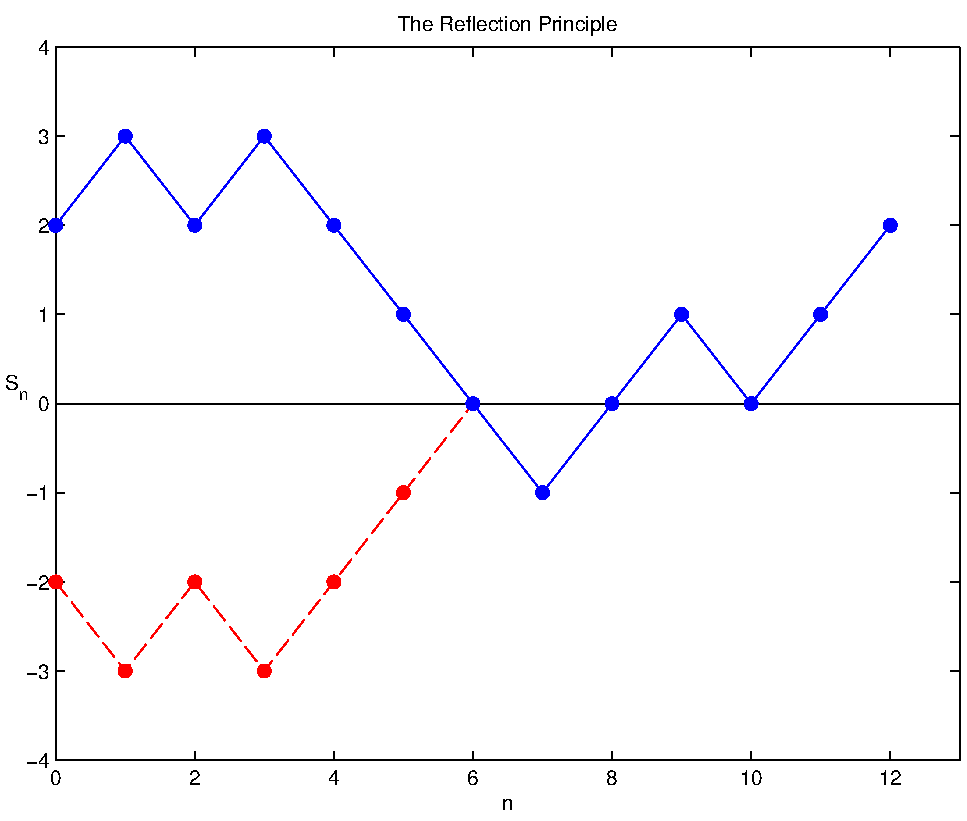
\includegraphics{reflection_principle}}
\caption{The Reflection Principle\label{reflection_principle}}
\end{figure}

%Let $a,b>0$ and define $C^{0}_n(a,b)$ to be the set of paths from $(0,a)$ to $(n,b)$ which contain a point of the form $(k,0)$, i.e.\ those trajectories which return to the (spatial) origin at some time step $k=0,1,2,\ldots,n$. We can use the reflection principle to show that the number of such paths is equal to the total number of paths from $(0,-a)$ to $(n,b)$.
%
%-------------------------
% theorem: reflection principle
\begin{theorem}
Let $a,b>0$, and let $C^{0}_n(a,b)$ be the set of paths from $(0,a)$ to $(n,b)$ which visit the (spatial) origin:% at some time step $k\in\{1,2,\ldots,n-1\}$,
\[
C^{0}_n(a,b) = \big\{\mathbf{x}\in C_n(a,b): x_k=a \text{ for some } k=1,2,\ldots,n-1\}.
\]
The number of such paths is equal to the total number of paths from $(0,-a)$ to $(n,b)$,
\[
|C^0_n(a,b)| = |C_n(-a,b)|.
\]
\end{theorem}
\begin{proof}
Each path from $(0,a)$ to $(n,b)$ intersects the horizontal axis at some earliest point $(k,0)$. If we reflect the segment of the path with $0\leq t\leq k$ in the horizontal axis, we obtain a path from $(0,a)$ to $(n,b)$ which intersects the horizontal axis. This operation puts the elements of $C^0_n(a,b)$ and $C_n(-a,b)$ in one-to-one correspondence, which proves the theorem.
\end{proof}

%For simplicity, we now focus our attention on simple random walks that start at the origin, i.e.\ those for which $X_0=0$.
%
%For $\ell > 0$, let $C^{*}_n(\ell)$ be the set of paths from $(0,0)$ to $(n,\ell)$ which do \emph{not} revisit the initial location $X_0=0$. 
%
%


%%--------------------------------------------------------------------------
%\subsubsection{The Ballot Theorem}
%
%For $b>a\geq 0$, let $C^{*}_n(a,b)$ to be the set of paths from $(0,a)$ to $(n,b)$ which do \emph{not} revisit the initial location $X_0=a$. 
%\[
%C^{*}_n(a,b) = \big\{\mathbf{x}\in C_n(a,b): x_k=0 \text{ for some } k=1,2,\ldots,n-1\}.
%\]

% ballot theorem
\begin{theorem}[The ballot theorem]
Let $b>a\geq 0$, and let $C^{*}_n(a,b)$ to be the set of paths from $(0,a)$ to $(n,b)$ which do \emph{not} revisit the initial location $X_0=a$, 
\[
C^{*}_n(a,b) = \big\{\mathbf{x}\in C_n(a,b): x_k=a \text{ for some } k=1,2,\ldots,n-1\}.
\]
The number of such paths is given by
\[
|C^{*}_n(a,b)| = \frac{b-a}{n} |C_n(a,b)|,
\]
where $C_n(a,b)$ is the set of all paths from $(0,a)$ to $(n,b)$.
\end{theorem}

%-------------------------
\begin{proof}
Without loss of generality, let $a=0$. The first step of all such paths must be to $(1,1)$, so by the reflection principle the number of such paths is
\begin{align*}
|C^{*}_n(0,b)|
	& = |C_{n-1}(1,b)| - |C^0_{n-1}(1,b)| \\
	& = |C_{n-1}(1,b)| - |C_{n-1}(-1,b)|
\end{align*}
The result then follows by the fact that the total number of paths $(0,0)$ to $(n,b)$ is equal to
\[
|C_n(0,b)| = \binom{n}{\frac{1}{2}(n+b)}
\]
and
\[
\begin{array}{lll}
|C_{n-1}(1,b)| 	& = \binom{n-1}{\frac{1}{2}(n+b)} 	& = \frac{n+b}{2n} |C_n(0,b)| \\
|C_{n-1}(-1,b)|	& = \binom{n-1}{\frac{1}{2}n+b-1}	& = \frac{n-b}{2n} |C_n(0,b)| \\
\end{array}
\]
\end{proof}

%-------------------------
% example
\begin{example}
In an election, candidate A scores $\alpha$ votes and candidate B scores $\beta$ votes, where $\alpha > \beta$. What is the probability that candidate $A$ was always ahead of candidate $B$ during the election? 
\begin{solution}
Assume that each possible combination of $\alpha$ votes for $A$ and $\beta$ votes for $B$ is equally likely.

\bigskip
After $n=\alpha+\beta$ steps, the required probability is the proportion of paths from $(0,0)$ to $(\alpha+\beta,\alpha-\beta)$ which do not re-visit the horizontal axis. By the ballot theorem, 
\[
\prob(\text{$A$ was always ahead of $B$}) = \frac{\alpha-\beta}{\alpha+\beta}.
\]
\end{solution}
\end{example}


%% thm: maximum
%\begin{theorem}
%Let $\{X_n\}$ be a symmetric simple random walk with $X_0=0$, and let $M_n=\max\{X_0,X_2,\ldots,X_n\}$. Then
%\[
%\prob(M_n\geq \ell)	= \prob(X_n=\ell) + \prob(X_n=\ell+1) 
%\]
%Note that only one of $\prob(X_n=\ell)$ and $\prob(X_n=\ell+1)$ is non-zero, the first if $n$ and $\ell$ are both odd or both even, and the second if one is odd and the other is even.
%\end{theorem}
%
%\begin{proof}
%Let $A_n(\ell)$ be the set of paths whose maximum is at least equal to $\ell$:
%\begin{align*}
%A_n(\ell) 
%	& = \{\mathbf{x}\in C_n: \max x_k \geq \ell, k=1,2,\ldots,n\} \\
%	& = \big\{\mathbf{x}\in C_n: x_k \geq \ell \text{ for at least one } k\in\{0,1,\ldots,n\}\big\}
%\end{align*}
%There are $2^n$ possible sample paths, all equally likely, so 
%\[
%\prob(M_n \geq \ell) = 2^{-n}|A_n(\ell)|.
%\]
%Let 
%\bit
%\it $A_n^{(1)}(\ell) = \big\{\mathbf{x}\in A_n(\ell): x_n > \ell\big\}$,
%\it $A_n^{(2)}(\ell) = \big\{\mathbf{x}\in A_n(\ell): x_n = \ell\big\}$,
%\it $A_n^{(3)}(\ell) = \big\{\mathbf{x}\in A_n(\ell): x_n < \ell\big\}$.
%\eit
%Then
%\[
%|A_n(\ell)| = |A_n^{(1)}(\ell)| + |A_n^{(2)}(\ell)| + |A_n^{(3)}(\ell)|
%\]
%
%By the reflection principle, the trajectories in $A_n^{(1)}(\ell)$ are in one-to-one correspondence with those in $A_n^{(3)}(\ell)$, so 
%\[
%|A_n(\ell)| = 2|A_n^{(1)}(\ell)| + |A_n^{(2)}(\ell)|
%\]
%
%Now, 
%\bit
%\it $A_n^{(1)}(\ell) = \cup_{k=\ell+1}^{\infty}\{\mathbf{x}: x_n=k\}$ and 
%\it $A_n^{(2)}(\ell) = \{\mathbf{x}: x_n=\ell\}.
%\eit
%
%There are $2^n$ sample paths, each equally likely, so
%\begin{align*}
%\prob(M_n\geq \ell)
%	& = 2\sum_{k=\ell+1}^{\infty}\prob(X_n=k) + \prob(X_n=\ell) \\
%	& = \sum_{k=\ell+1}^{\infty}\prob(X_n=k) + \sum_{k=\ell}^{\infty}\prob(X_n=\ell) \\
%\end{align*}
%
%Hence,
%\begin{align*}
%\prob(M_n = \ell) 
%	& = \prob(M_n\geq \ell) - \prob(M_n\geq \ell+1) \\
%	& = \prob(M_n\geq \ell) - \prob(M_n\geq \ell+1) \\
%	& = \left(\sum_{k=\ell+1}^{\infty}\prob(X_n=k) + \sum_{k=\ell}^{\infty}\prob(X_n=k)\right)
%			- \left(\sum_{k=\ell+2}^{\infty}\prob(X_n=k) + \sum_{k=\ell+1}^{\infty}\prob(X_n=k)\right) \\
%	& = \sum_{k=\ell}^{\infty}\prob(X_n=k) - \left(\sum_{k=\ell+2}^{\infty}\prob(X_n=k) \\
%	& = \prob(X_n=\ell)\right) + \prob(X_n=\ell+1)\right) \\
%\end{align*}
%
%\end{proof}

%-----------------------------
\subsection{Hitting times}
Let $X_n=\sum_{k=1}^{n}\xi_k$ be a simple random walk with $X_0=0$. The \emph{first hitting time} at level $\ell$ is the time at which the trajectory first reaches level $\ell\in\N$,
\[
T_{\ell} = \min\{n: X_n=\ell\}
\]
If $T_{\ell}=n$, we must have that (1) $X_n = \ell$ and (2) $X_k < \ell$ for all $k=0,1,2,\ldots,n-1$.

\begin{example}[Gambler's ruin]
A gambler starts with $\pounds x$ and plays a game in which a fair coin is tossed repeatedly. Each time, if the coin shows heads then he wins $\pounds 1$, but if the coin shows tails he loses $\pounds 1$. The gambler stops when either he goes bankrupt or otherwise reaches some pre-determined amount $\pounds a$. Find the probability that the gambler goes bankrupt.
%Show that the probability that the gambler goes bankrupt is equal to $(a-x)/x$.
\end{example}

\begin{solution}
Let $X_n$ denote the gambler's \emph{winnings} after $n$ steps. The sequence $X_0,X_1,X_2,\ldots$ can be modelled by a symmetric simple random walk starting at $X_0=0$, with
\[
X_n = \sum_{k=1}^n \xi_k \quad\text{where $\prob(\xi_k=1)=1/2$ and $\prob(\xi_k=-1)=1/2$.} 
\]
Let $T$ be the (random) time at which the game stops:
\bit
\it $T=\min\{T_0,T_a\}$ where $T_0$ and $T_a$ are the hitting times of levels $0$ and $a$ respectively.
\eit

Consider the random variable $X_T = \sum_{k=1}^{T}\xi_k$, the gambler's winnings at the random time $T$.
\bit
\it Clearly $X_T = -x$ or $X_T = a-x$. 
\it Let $p_0=\prob(X_T = -x)$ and $p_1=\prob(X_T = a-x)$. 
\eit

Let $\xi$ be a random variable with $\prob(\xi_k=1)=1/2$ and $\prob(\xi_k=-1)=1/2$, and let $\xi_1,\xi_2,\ldots$ be independent increments from the distribution of $\xi$. By Corollary~\ref{cor:GF-NofX} (Wald's identity),
\[
\expe(X_T) = \expe(T)\expe(\xi) = \expe(T)\times 0 = 0,
\]
We also know that $\expe(X_T) = (-x)p_0 + (a-x)p_a$, so $xp_0 = (a-x)p_a$. Thus, using the fact that $p_0+p_a=1$, we obtain
\[
p_0 = \frac{a-x}{a} \quad\text{and}\quad p_1 = \frac{x}{a}.
\] 
Note that we have assumed that $\expe(T)<\infty$, which requires that $\prob(T<\infty)=1$.

\end{solution}

%-----------------------------

\begin{theorem}
Let $\{X_n\}$ be a simple random walk with $X_0=0$, and let $T$ be the first hitting time at level $\ell=1$. The PMF of $T$ is given by the following recursive formula,
\[
p_n = q\sum_{k=1}^{n-2}p_{k}p_{n-k-1}, \qquad p_0=0, p_1=p, q=1-p..
\]
where $p_n = \prob(T=n)$.
\end{theorem}
\begin{proof}
\bit
\it We cannot move from $0$ to $1$ in an even number of steps, so $p_{2n}=0$ for $n\in\Znn$.
\it For $n=1$, the first step must be upwards, so $p_1=p$.
\it For $n>1$, the first step must be downwards (which occurs with probability $q$), and then we need to climb from $-1$ to $0$, and then from $0$ to $1$. 
\eit
\begin{align*}
\prob(T=n)
	& = q\sum_{k=1}^{n-2}\prob(\text{$k$ steps to first hit $0$ from $-1$, and $n-k-1$ steps to first hit 1 from $0$}) \\
	& = q\sum_{k=1}^{n-2}\prob(\text{$k$ steps to first hit $0$ from $-1$})\prob(\text{$n-k-1$ steps to first hit $1$ from $0$}) \\
	& = q\sum_{k=1}^{n-2}\prob(\text{$k$ steps to first hit $1$ from $0$})\prob(\text{$n-k-1$ steps to first hit $1$ from $0$}) \\
	& = q\sum_{k=1}^{n-2}p_{k}p_{n-k-1}
\end{align*}
\end{proof}

\begin{theorem}
The PGF of $T$ is given by $\displaystyle G(t) = \frac{1 - \sqrt{1-4pqt^2}}{2qt}$.
\end{theorem}

\begin{proof}
Let $G(t) = \sum_{k=0}^{\infty} p_k t^k$ be the PGF of $T$. The square of the PGF can be written as 
\[
G(t)^2 = \sum_{k=0}^{\infty} \left(\sum_{i=0}^{k} p_ip_{k-i}\right) t^k
\]
Because $p_0=0$ and $p_{k+1}=q\sum_{i=1}^{k-1}p_{i}p_{k-i}$, the inner sum can be written as
\[ 
\sum_{i=0}^{k} p_ip_{k-i} 
	= \sum_{i=1}^{k-1} p_ip_{k-i} 
	=  q^{-1}p_{k+1} \quad\text{for $k\geq 2$.}
\]
(and zero for $k=0$ and $k=1$). Hence,
\[
G(t)^2 = q^{-1}\sum_{k=2}^{\infty} p_{k+1} t^{k+1} = G(t) - pt
\]
so
\[
qtG(t)^2 = \sum_{k=2}^{\infty} p_{k+1} t^{k+1} = \sum_{k=0}^{\infty} p_k t^k - pt = G(t) - pt.
\]
Thus we obtain a quadratic equation for $G(t)$,
\[
qtG(t)^2 - G(t) + pt = 0
\]
and solving for $G(t)$ we obtain
\[
G(t) = \frac{1\pm\sqrt{1-4pqt^2}}{2qt}
\]
For any PGF we must have that $G(t)\leq 1$, so we conclude that
\[
G(t) = \frac{1 - \sqrt{1-4pqt^2}}{2qt}
\]
\end{proof}

\begin{remark}
The probabilities $p_n$ can be computed by taking successive derivatives of $G(t)$ and evaluating these at $t=1$. An explicit expression is given by
\[
p_{2n-1} = p^n q^{n-1}\frac{2}{n}\binom{2n-3}{n-2}.
\]
This result can also be obtained by the reflection principle. 
\end{remark}

% probability that we don't hit level 1 at all
\begin{remark}
Since $G(1)=\sum_{k=0}^{\infty}p_k$ we might be inclined to think that $G(1)=1$. In fact,
\[
G(1) = \frac{1 - \sqrt{1-4pq}}{2q} = \frac{1-|p-q|}{2q} 
	= \begin{cases} 
		1 	& \text{ for $p\geq 1/2$,} \\
		p/q & \text{ for $p < 1/2$.}
	\end{cases}
\]
Thus if $p<q$ we see that $G(1)<1$, which show that the random walk might never reach level $1$ when the probability of a positive step is smaller than the probability of a negative step. In this case, $G(1)=\sum_{k=0}^{\infty}p_k = \prob(T<\infty)$, so $\prob(T=\infty)>0$. It is a remarkable fact that if $p=1/2$, the random walk will \emph{always} hit level $1$ sooner or later, but this need not happen if $p<1/2$. This behaviour is known as \emph{criticality} -  many systems exhibit qualitatively different behaviour when the value of a parameter $p$ lies either side of some critical value $p_c$.
\end{remark}

% expected first hitting time
\begin{remark}
We can compute the \emph{expected} time before the random walk hits $1$ for the first time. If $p<1/2$ then $\prob(T=\infty)>0$ so $\expe(T)=\infty$. For the case $p\geq 1/2$, note that
\[
G'(t) = \frac{2p}{\sqrt{1-4pqt^2}} - \frac{1-\sqrt{1-4pqt^2}}{2qt^2}.
\]
\[
\begin{array}{lcl}
p=1/2:	& \qquad	& \expe(T) = \lim_{t\nearrow 1}G'(t)	= \lim_{t\nearrow 1}\left(\frac{1}{\sqrt{1-t^2}} - \frac{1-\sqrt{1-t^2}}{t^2}\right) = +\infty. \\
p>1/2:	&			& \expe(T) = \lim_{t\nearrow 1}G'(t) = \frac{1}{p-q}.
\end{array}
\]
\end{remark}

%==========================================================================
\begin{exercise}
Consider a simple random walk $X_0,X_1,X_2,\ldots$ with $X_0=0$. Let $q$ be the probability that the random walk eventually returns to the starting position $X_0$. If $q=1$, position $X_0$ is called \emph{recurrent}; if $q<1$, position $X_0$ is called \emph{transient}. Show that $X_0$ is transient if and only if $\sum_{n=1}^{\infty} \prob(X_n = 0) < \infty$. [\textit{Hint}: find expressions for the expected number of times that $X_0$ is re-visited.]
\begin{answer}
Let 
\[
I_n = \begin{cases}
1 & \text{if } X_n = 0 \\
0 & \text{otherwise.}
\end{cases}
\]
and let $N = \sum_{n=1}^{\infty} I_n$ be the number of times that state $X_0=0$ is revisited.

The expected value of $N$ is given by
\[
\expe(N) 
	= \expe\left(\sum_{n=1}^{\infty} I_n\right) 
	= \sum_{n=1}^{\infty} \expe(I_n)
	= \sum_{n=1}^{\infty} \prob(X_n = 0)
\]

The expected value of $N$ is also given by
\begin{align*}
\expe(N)
	& = \sum_{k=1}^{\infty} k\prob(N=k) \\
	& = \sum_{k=1}^{\infty} \big[ k\prob(N\geq k) - k\prob(N\geq k+1)\big] \\
	& = \sum_{k=1}^{\infty} k\prob(N\geq k) - \sum_{k=2}^{\infty} (k-1)\prob(N\geq k) \\
	& = \sum_{k=1}^{\infty} \prob(N\geq k) \\
	& = \sum_{k=1}^{\infty} q^k 
\end{align*}
where the last equality follows by the fact that every return occurs independently with probability $q$. Combining these results, we get
\[
\sum_{n=1}^{\infty}\prob(X_n=0) = \sum_{k=1}^{\infty} q^k
\]
which diverges if $q=1$, and converges if $q<1$. Thus the random walk is recurrent precisely when $\sum_{n=1}^{\infty} \prob(X_n = 0)$ is infinite.
\end{answer}
\end{exercise}

%% reflection principle (first passage time distribution)
%%==========================================================================
%\begin{exercise}
%Consider a simple random walk $X_0,X_1,X_2,\ldots$ with $X_0=0$. Let $T_{\ell}$ be the first hitting time at level $\ell$, defined by $T_{\ell} = \min\{n\geq 0\,:\, X_n = \ell\}$. Use the reflection principle to show that the distribution of $T_{\ell}$ satisfies 
%\[
%\prob(T_{\ell}\leq n) = \prob(X_n = \ell) + 2\prob(X_n > \ell).
%\]
%\begin[answer}
%Consider the sequence $X_n^{*}$ defined by
%\[
%X_n^{*} = \begin{cases}
%	X_n			& \text{if } n\leq\tau(m) \\
%	2m - X_n		& \text{if } n\geq\tau(m)
%\end{cases}	
%\]
%By the reflection principle, $X_n^{*}$ is a simple random walk starting from $X_0^{*}=0$.
%%
%Consider the event $\tau(m)\leq n$. If this event occurs, $X_n$ and $X_n^{*}$ are on opposite sides of $m$ (unless they are both at $m$), and correspond under reflection. Since both processes are simple random walks starting at zero,
%\[
%\prob(X_n^{*} = m+k) = \prob(X_n = m+k) \qquad\text{for all } k\geq 0
%\]
%
%If $k\geq 0$, the event $X_n=m+k$ is impossible unless $\tau(m)\leq n$, so
%\begin{align*}
%\prob(X_n = m+k) 
%	& = \prob\big(X_n 	= m+k \text{ and } \tau(m)\leq n\big) \\
%	& = \prob\big(X_n^{*}= m+k \text{ and } \tau(m)\leq n\big) \\
%	& = \prob\big(X_n 	= m-k \text{ and } \tau(m)\leq n\big) \\
%\end{align*}
%and therefore
%\begin{align*}
%\prob\big(\tau(m)\leq n\big) 
%	& = \sum_{k=-\infty}^{\infty} \prob\big(X_n = m+k\text{ and }\tau(m)\leq n\big) \\
%	& = \prob(X_n = m) + 2\prob(X_n > m)
%\end{align*}
%as required.
%\end{answer}
%\end{exercise}


%-------------------------------------------------
\section{Branching processes}\label{sec:branching}
In Victorian England, several aristocratic families realised that their family names could become extinct. In 1873, Sir Francis Galton posed the following question in the \textit{Educational Times}:
\begin{quote}
How many male children (on average) must each generation of a family have for the family name to continue in perpetuity?
\end{quote}
The first complete answer was put forward by Reverend Henry Watson. Galton and Watson published a paper entitled \textit{On the probability of extinction of families} in 1874. Their model is as follows.

\ben
\it A population starts with a single individual, $Z_0=1$
\it At time $n=1$, this individual gives birth to $Z_1$ offspring, where $Z_1\in\{0,1,2,\ldots\}$, then dies.
\it If $Z_1=0$, the population is extinct and $Z_n=0$ for all $n\geq 2$.
\it If $Z_1>0$, each of the $Z_1$ individuals in the first generation gives birth to a random number of offspring at time $n=2$: the first has $Z_{1,1}$ offspring, the second has $Z_{1,2}$ offspring, ..., and the has last $Z_{1,Z_1}$ offspring. 
\it Assume that every individual in every generation has the same offspring distribution, and the number of offpring born to any individual is independent of the number born to any other individual.
\it The total number of individuals in the second generation is
\[
Z_2 = \sum_{k=1}^{Z_1} Z_{1,k}.
\]
\it The third, fourth, fifth etc. generations are produced in the same way.
\it If it happens that $Z_m=0$ for some $m$ then $Z_n=0$ for all $m\geq n$, and the population is \emph{extinct}.
\een

\begin{definition}
A random process $Z_0,Z_1,Z_2\ldots$ with the properties described above is called a \emph{simple branching process} (or Galton-Watson process).
\end{definition}

The offspring distribution determines the evolution of a branching process. Galton's question is to find conditions on the offspring distribution under which
\[
\prob\big(Z_n\geq 1 \text{ for all } n=0,1,2,\ldots\big) = 1.
\]

Let $p_0,p_1,p_2,\ldots$ denote the offspring distribution, and let $G(t)=\sum_{k=1}^{\infty}p_k t^k$ be its PGF.

\begin{theorem}
The PGF of $Z_n$ is the $n$-fold composition of $G(t)$ with itself,
\[
G_{Z_n}(t) = \underbrace{G(G(\ldots G(t)\ldots))}_{\text{$n$ times}} \quad\qquad (n\geq 1). 
\]
\begin{proof}
For $n=1$, $Z_1$ has distribution $p_0,p_1,p_2,\ldots$ so $G_{Z_1}(t) = G(t)$.
Suppose the statement holds for some $n\in\N$. Then
\[
Z_{n+1} = \sum_{i=1}^{Z_n} Z_{n,i}.
\]
is a random sum of $Z_n$ independent variables with PMF $p_0,p_1,\ldots$, and where the number of summands $Z_n$ is independent of the summands $Z_{n,1},Z_{n,2},\ldots,Z_{n,Z_n}$.

\bigskip
Hence, by Theorem~\ref{thm:GF-NofX},
\[
G_{Z_{n+1}}(t) = G_{Z_n}\big[G(t)\big]
\]
and by the inductive hypothesis, 
\[
G_{Z_{n+1}}(t) = \underbrace{G(G(\ldots G(t)\ldots))}_{\text{$n+1$ times}}
\]
as required.
\end{proof}
\end{theorem}

%-------------------------
% theorem
\begin{theorem}
Let $Z_0,Z_1,Z_2,\ldots$ be a simple branching process, and let $\mu$ and $\sigma^2$ be the mean and variance of its offspring distribution. Then $\expe(Z_n)=\mu^n$ and 
\[
\var(Z_n) 
	= \sigma^2\mu^n(1+\mu+\mu^2+\cdots+\mu^n)
	= \begin{cases}
		\sigma^2(n+1)							& \text{if } \mu=1,\\
		\sigma^2\mu^n\left(\frac{1-\mu^{n+1}}{1-\mu}\right)	& \text{if } \mu\neq 1.
	\end{cases}		
\]
\end{theorem}
%-------------------------
\begin{proof}
For brevity, let $G_n(t)$ denote the PGF $G_{Z_n}(t)$ of $Z_n$
\ben
\it % mean
To find the mean, differentiate $G_n(t) = G\big(G_{n-1}(t)\big)$,
\[
G'_n(t) = G'\big(G_{n-1}(t)\big)G'_{n-1}(t).
\]
Evaluating this at $t=1$, and using the fact that $G_{n-1}(1)=1$,
\[
\expe(Z_n) = G'_n(1) = G'(1)G'_{n-1}(1) = \mu\expe(Z_{n-1})
\]
The result then follows by induction.
\it % variance
To find the variance, differentiate $G_n(s)=G\big(G_{n-1}(s)\big)$ twice to obtain
\[
G''_n(1) = G''(1)G'_{n-1}(1)^2 + G'(1)G''_{n-1}(1)
\]
and substitute in the expression $\var(Z_n) = G''_n(1) + G'_n(1) - G'_n(1)^2$.
\een
\end{proof}

%-----------------------------
\subsection{Extinction probability}

The event that the population becomes extinct can be written as
\[
E = \big\{\omega\in\Omega:Z_n(\omega)=0 \text{ for some } n\in\N\}.
\]
This can be written as the union of an expanding sequence of events $E_1\subseteq E_2\subseteq\ldots$,
\[
E = \medcup_{n=1}^{\infty} E_n \quad\text{where}\quad E_n = \{\omega\in\Omega:Z_n(\omega)=0\}.
\]
By the continuity of probability measures, the \emph{extinction probability} is 
\[
\prob(E) = \lim_{n\to\infty}\prob(E_n).
\]
Using the fact that $\prob(E_n) = \prob(Z_n=0) = G_{Z_n}(0)$,
\[
\prob(E) = \lim_{n\to\infty}G_{Z_n}(0) = \lim_{n\to\infty} \underbrace{G(G(\ldots G(0)\ldots))}_{\text{$n$ times}}
\]

Remarkably, the extinction probability $\prob(E)$ can be computed even when $G_{Z_n}$ is not known explicitly.
\begin{theorem}
The extinction probability is the smallest non-negative solution of the so-called \emph{extinction equation},
\[
x = G(x)
\]
where $G$ is the PGF of the offspring distribution.
\end{theorem}

\begin{proof}
Let $e=\prob(E)$ be the extinction probability. First we show that $e$ is a solution of $x=G(x)$. Let
\[
x_n = \underbrace{G(G(\ldots G(0)\ldots))}_{\text{$n$ times}}
\]
Then (1) $e=\lim_{n\to\infty}x_n$ and (2) $G(x_n) = x_{n+1}$, so
\[
e 	= \lim_{n\to\infty}x_n 
	= \lim_{n\to\infty}x_{n+1} 
	= \lim_{n\to\infty}G(x_n) 
	= G(\left(\lim_{n\to\infty}x_n\right)
	= G(e),
\]
where we have used the fact that $G$ is a continuous function.

To show that $e=\prob(E)$ is the smallest solution, let $e'$ be another solution of $x=G(x)$ in $[0,1]$. Since $e'\geq 0$ and $G(t)$ is a non-decreasing function,
\[
G(0) \leq G(e') = e'.
\]
Applying $G$ to both sides, since $G(t)$ is increasing,
\[
G(G(0)) \leq G(G(e')) = G(e') = e'.
\]
Repeating this procedure, we get
\[
\prob(E_n) = \underbrace{G(G(\ldots G(0)\ldots))}_{\text{$n$ times}} \leq e'.
\]
Hence,
\[
e =\prob(E) = \lim_{n\to\infty}\prob(E_n) \leq \lim_{n\to\infty} e' = e',
\]
so $e$ is not larger than any other solution $e'$ of $x=G(x)$.
\end{proof}

%-------------------------------------------------
\section{Martingales}\label{sec:martingales}
%-------------------------
% definition
\begin{definition}
A random process $X_0,X_1,\ldots$ is called a \emph{martingale} with respect to the sequence of random variables $\xi_1,\xi_2,\ldots$ if 
\ben
\it $\expe(|X_n|) < \infty$ and
\it $\expe(X_{n+1}|\xi_1,\ldots,\xi_n) = X_n$.
\een
\bit
\it A \emph{sub-martingale} has $\expe(X_{n+1}|\xi_1,\ldots,\xi_n) \geq X_n$ (the process tends to increase over time).
\it A \emph{super-martingale} has $\expe(X_{n+1}|\xi_1,\ldots,\xi_n) \leq X_n$ (the process tends to decrease over time).
\eit
\end{definition}

%-------------------------
% example
\begin{example}[Random walk]
Let $X_n=X_0+\sum_{k=1}^n \xi_n$ be a symmetric simple random walk (so $\prob(\xi_k=1)=\prob(\xi_k=-1) = 1/2$). Show that $\{X_n\}$ is a martingale with respect to the increments $\xi_1,\xi_2,\ldots$.
\begin{solution}
For the first condition, $\expe(|\xi_i|)=1$ so
\[
\expe(|X_n|) = \expe\left(\left|\sum_{i=1}^{n} \xi_i\right|\right) \leq \sum_{i=1}^{n} \expe(|\xi_i|) < \infty.
\]
For the second condition,
\begin{align*}
\expe(X_{n+1}|\xi_1,\xi_2,\ldots,\xi_n)
	& = \expe(\xi_1+\xi_2\ldots+\xi_{n+1}|\xi_1,\ldots,\xi_n) \\
	& = \expe(\xi_1|\xi_1,\ldots,\xi_n) + \expe(\xi_2|\xi_1,\ldots,\xi_n) + \ldots + \expe(\xi_{n+1}|\xi_1,\ldots,\xi_n) \\
	& = \expe(\xi_1|\xi_1) + \expe(\xi_2|\xi_2) + \ldots + \expe(\xi_n|\xi_n) + \expe(\xi_{n+1}) \qquad \text{by independence} \\
	& = \xi_1 + \xi_2 + \ldots + \xi_n + 0 \\
	& = X_n.
\end{align*}
\end{solution}
\end{example}

%-------------------------
% example
\begin{example}[Sub-martingale]
Let $\xi_1,\xi_2,\ldots$ be independent random variables with zero means, finite variances and partial sums $X_n=\sum_{i=1}^n \xi_i$. Show that $X_n^2$ is a sub-martingale with respect to $\xi_1,X_2,\ldots$.
\begin{solution}
Since $X^2_{n+1} = (X_n + \xi_{n+1})^2$, 
\begin{align*}
\expe(X^2_{n+1}|\xi_1,\xi_2,\ldots,\xi_n)
	& = \expe(X_n^2 + 2X_n\xi_{n+1} + \xi_{n+1}^2 | \xi_1,\ldots,\xi_{n}) \\
	& = X^2_n + 2\expe(\xi_{n+1})\expe(X_n | \xi_1,\ldots,\xi_n) + \expe(\xi_{n+1}^2) \qquad \text{by independence,} \\
	& = X^2_n + \expe(\xi_{n+1}^2) \geq T_n \qquad\text{because $\expe(\xi_{n+1})=0$.}
\end{align*}	
Since $\xi_{n+1}^2>0$, $\expe(X^2_{n+1}|\xi_1,\xi_2,\ldots,\xi_n)\geq X^2_n$, so $X^2_n$ is a sub-martingale.
\end{solution}
\end{example}

%-------------------------
% thm: MCT
\begin{theorem}[Martingale Convergence Theorem]
Let $X_0,X_1,\ldots$ be a martingale such that $\expe(|X_n|)$ is bounded for all $n=0,1,2,\ldots$. Then there exists a finite random variable $X$ such that $X_n\to X$ with probability one as $n\to\infty$.
\end{theorem}

The MCT can be used to prove the following remarkable theorem.
%-------------------------
% example (application of MCT}
\begin{theorem}
A symmetric simple random walk on $\Z$ will visit every point with probability 1.
\end{theorem}
\begin{proof}
Let $X_0=0$ and $b\in\Z$, and suppose (without loss of generality) that $b<0$. Let $T$ be the first time $n$ for which $X_n=b$, and consider the corresponding \emph{stopped process} $\tilde{X}_0,\tilde{X}_1,\tilde{X}_2,\ldots$ defined by $\tilde{X}_n = X_{\min\{n,T\}}$.
\bit
\it The stopped process remains in position $b$ from time $T$ onwards.
\eit

It is easy to show that $\tilde{X}_n$ is a martingale, and because $\tilde{X}_n - b$ is non-negative, $\expe(|\tilde{X}_n - b|) = \expe(\tilde{X}_n - b) < \infty$.

\bigskip
By the Martingale Convergence Theorem, the limit $\tilde{X} = \lim_{n\to\infty}\tilde{X}_n$ exists and is finite with probability one.
\bit
\it In particular, $|\tilde{X}_{n+1} - \tilde{X}_n|$ converges to zero, and must therefore  be less than 1 for large $n$.
\it However $|\tilde{X}_{n+1} - \tilde{X}_n| = 1$ whenever $n < T$.
\it Thus we have $T<\infty$, and hence $X_n = b$ for some $n$.
\eit
\end{proof}

% ex: branchingn process
\begin{exercise}
Let $Z_0,Z_1,Z_2,\ldots$ be a simple branching process with $Z_0=1$. Show that the sequence $W_1,W_2,\ldots$ with $W_n=Z_n/\expe(Z_n)$ is a martingale with respect to $Z_1,Z_2,\ldots$.
\begin{answer}
Conditioned on $Z_n=z_n$, the number $Z_{n+1}$ is the sum of $z_n$ independent familiy sizes,
\[
\expe(Z_{n+1}: Z_n=z_n) = \mu z_n
\]
where $\mu$ is the expected family size. By the Markov property,
\[
\expe(Z_{n+1}: Z_1,Z_2,\ldots,Z_n) = \mu Z_n
\]
Since $\expe(Z_n)=\mu^n$, we conclude that
\[
\expe(W_{n+1}: Z_1,Z_2,\ldots,Z_n) = W_n
\]
as required.
\end{answer}
\end{exercise}

%==========================================================================
\begin{exercise}
An urn contains one red ball and one green ball. At each time step, we choose one ball uniformly at random from the urn, and replace it along with another ball of the same colour. Let $R_n$ and $G_n$ respectively denote the number of red balls and green balls after $n$ steps, and let $M_n$ denote the fraction of green balls in the urn.
\ben
\it Show that $M_n$ is a martingale.
\it Show that $M_n$ converges to a finite limit with probability 1 as $n\to\infty$
\een
\begin{answer}
\ben
\it % (a)
$M_n$ is a martingale because
\begin{align*}
\expe(M_{n+1} | R_0,G_0,\ldots,R_n,G_n)
	& = \left(\frac{R_n}{R_n+G_n}\right)\left(\frac{G_n}{R_n+G_n+1}\right)
	  + \left(\frac{G_n}{R_n+G_n}\right)\left(\frac{G_n+1}{R_n+G_n+1}\right) \\
	& = \frac{G_n}{R_n+G_n} \\
	& = M_n
\end{align*}		
\it % (b)
Since $M_n\geq 0$ is bounded for all $n\in\N$, it follows by the martingale that there exists a finite random variable $M$ such that $M_n\to M$ with probability one as $n\to\infty$. In fact, it can be shown that
\[
\prob(G_n = m+1) = \binom{m}{n}\frac{m!(n-m)!}{(n+1)!} = \frac{1}{n+1}
\]
and hence
\[
\prob(M_n\leq x) = \frac{\lfloor x(n+2)-1\rfloor}{n+1} \to x \quad\text{as }n\to\infty
\]
Thus the distribution of $M_n$ approaches a uniform distribution on $[0,1]$ as $n\to\infty$.
\een
\end{answer}
\end{exercise}

\endinput

% !TEX root = main.tex
%=====================================================================
\chapter{Bayesian Inference}\label{chap:randomprocesses}

%----------------------------------------------------------------------
%\section{The Bayesian approach}
%----------------------------------------------------------------------

So far we have looked at \emph{frequentist inference}, which assumes that an unknown parameter $\theta$ has a fixed (but unknown) value. 
\bit
\it The PMF/PDF of an observation is written as $f(x;\theta)$.
\it The likelihood function is written as $L(\theta;x)$.
\it Estimators such as the MME and MLE claim to estimate the `true' value of $\theta$.
\eit

For \emph{Bayesian inference}, we instead think of an unknown parameter $\theta$ as a \emph{random variable}.
\bit
\it The PMF/PDF of an observation is written as $f(x|\theta)$.
\it The likelihood function of is written as $L(\theta|x)$.
\it We seek to estimate the distribution of $\theta$.
\eit

%----------------------------------------------------------------------
\section{Bayes' theorem}
%----------------------------------------------------------------------

% events
If the events $A_1,A_2,\ldots$ form a partition of event $B$, Bayes' theorem states that
\[
\prob(A_j|B) 
%	= \frac{\prob(B|A_j)\prob(A_j)}{\prob(B)} 
	= \frac{\prob(B|A_j)\prob(A_j)}{\sum_k \prob(B|A_k)\prob(A_k)}.
\]

% discrete
Let $X$ and $Y$ be discrete random variables taking values in the sets $\{x_1,x_2,\ldots\}$ and $\{y_1,y_2,\ldots\}$ respectively. Because the events $\{Y=y_1\},\{Y=y_2\},\ldots$ form a partition of the event $\{X=x_i\}$, we have % so applying Bayes' theorem we obtain
\[
\prob(Y=y_j|X=x_i) 
%= \frac{\prob(X=x_i|Y=y_j)\prob(Y=y_j)}{\prob(X=x_i)}
= \frac{\prob(X=x_i|Y=y_j)\prob(Y=y_j)}{\sum_k \prob(X=x_i|Y=y_k)\prob(Y=y_k)}.
\]
To avoid cluttering the notation with subscripts, we write this as
\[
\prob(Y=y|X=x) 
%= \frac{\prob(X=x|Y=y)\prob(Y=y)}{\prob(X=x)}
= \frac{\prob(X=x|Y=y)\prob(Y=y)}{\sum_y \prob(X=x|Y=y)\prob(Y=y)},
\]
where the sum in the denominator is taken over the range of $Y$.
In terms of PMFs, this becomes
\[
f_{Y|X}(y|x) 
%= \frac{f_{X|Y}(x|y)f_Y(y)}{f_X(x)}
= \frac{f_{X|Y}(x|y)f_Y(y)}{\sum_y f_{X|Y}(x|y)f_Y(y)}.
\]

% continuous
This extends directly to the case of continuous random variables, the only difference being that the denominator (which is the marginal PDF of $X$) is expressed by an integral:
\[
f_{Y|X}(y|x) 
%= \frac{f_{X|Y}(x|y)f_Y(y)}{f_X(x)}
= \frac{f_{X|Y}(x|y)f_Y(y)}{\int f_{X|Y}(x|y)f_Y(y)\,dy}.
\]

% parameter estimation
For Bayesian inference, the unknown parameter $\theta$ takes the role of $Y$ in the above formulation. To simplify the notation we denote the PMF/PDF of $\theta$ by the symbol $\pi$: 
\[
\pi(\theta|\mathbf{x}) = \left\{\begin{array}{ll}
	\displaystyle\frac{f(\mathbf{x}|\theta)\pi(\theta)}{\sum_{\theta}f(\mathbf{x}|\theta)\pi(\theta)} 			& \text{\quad ($\theta$ discrete)}, \\[5ex]
	\displaystyle\frac{f(\mathbf{x}|\theta)\pi(\theta)}{\int f(\mathbf{x}|\theta)\pi(\theta)\,d\theta} 	& \text{\quad ($\theta$ continuous)}.
\end{array}\right.
\]

This can also be expressed in terms of likelihood functions,
\[
\pi(\theta|\mathbf{x}) = \left\{\begin{array}{ll}
	\displaystyle\frac{L(\theta|\mathbf{x})\pi(\theta)}{\sum_{\theta}L(\theta|\mathbf{x})\pi(\theta)} 			& \text{\quad ($\theta$ discrete)}, \\[5ex]
	\displaystyle\frac{L(\theta|\mathbf{x})\pi(\theta)}{\int L(\theta|\mathbf{x})\pi(\theta)\,d\theta} 	& \text{\quad ($\theta$ continuous)}.
\end{array}\right.
\]

%----------------------------------------------------------------------
\section{The prior and posterior distributions}
%----------------------------------------------------------------------

%----------------------------------------------------------------------
\subsection*{The prior distribution}
%----------------------------------------------------------------------
% prior
Suppose we have an initial estimate for distribution of $\theta$, perhaps obtained as a result of some preliminary experiments. 
\bit
\it This is called the \emph{prior distribution} of $\theta$, which we denote by $\pi_0(\theta)$.
\eit

An initial point estimate of $\theta$ can be computed from the prior distribution, for example
\bit
\it by the \emph{mean} of the prior distribution: $\hat{\theta} = \expe\big[\pi_0(\theta)\big]$ or
\it by the \emph{mode} of the prior distribution: $\hat{\theta} = \argmax_{\theta}\big[\pi_0(\theta)\big]$.
\eit

If we have no prior knowledge, we should initially consider every value of $\theta$ to be equally likely. For example, if $\theta$ is continuous and all we know is that $\theta$ belongs to some interval $[a,b]$, we should adopt the \emph{uniform} distribution over $[a,b]$ as the prior distribution of $\theta$,
\[
\pi_0(\theta) = \left\{\begin{array}{ll}
	1/(b-a)	& \text{if } a\leq\theta\leq b, \\
	0	& \text{otherwise.}
\end{array}\right.
\]
In this context, the uniform distribution is often called the \emph{na\"{\i}ve} or \emph{non-informative} prior.

%----------------------------------------------------------------------
\subsection*{The posterior distribution}
%----------------------------------------------------------------------
% posterior
Suppose we now obtain some sample data $\mathbf{x}=(x_1,\ldots,x_n)$. 
\bit
\it Bayes' theorem can be used to combine the prior distribution with the data.
\it This yields an updated PMF/PDF $\pi_1(\theta)$, called the \emph{posterior distribution} of $\theta$.
\eit

By Bayes' theorem, 
%\[
%\pi_1(\theta|\mathbf{x}) = \left\{\begin{array}{ll}
%	\displaystyle\frac{f(\mathbf{x}|\theta)\pi_0(\theta)}{\sum_{\theta}f(\mathbf{x}|\theta)\pi_0(\theta)} 			& \text{\quad ($\theta$ discrete)}, \\[3ex]
%	\displaystyle\frac{f(\mathbf{x}|\theta)\pi_0(\theta)}{\int_{\theta}f(\mathbf{x}|\theta)\pi_0(\theta)\,d\theta} 	& \text{\quad ($\theta$ continuous)}.
%\end{array}\right.
%\]
%
%This can also be expressed in terms of likelihood functions,
%\[
%\pi_1(\theta|\mathbf{x}) = \left\{\begin{array}{ll}
%	\displaystyle\frac{L(\theta|\mathbf{x})\pi_0(\theta)}{\sum_{\theta}L(\theta|\mathbf{x})\pi_0(\theta)} 			& \text{\quad ($\theta$ discrete)}, \\[3ex]
%	\displaystyle\frac{L(\theta|\mathbf{x})\pi_0(\theta)}{\int_{\theta}L(\theta|\mathbf{x})\pi_0(\theta)\,d\theta} 	& \text{\quad ($\theta$ continuous)}.
%\end{array}\right.
%\]

\[
\pi_1(\theta|\mathbf{x}) 
	= \frac{f(\mathbf{x}|\theta)\pi_0(\theta)}{\sum_{\theta}f(\mathbf{x}|\theta)\pi_0(\theta)}
\qquad\text{or}\qquad
\pi_1(\theta|\mathbf{x}) 
	= \frac{f(\mathbf{x}|\theta)\pi_0(\theta)}{\int f(\mathbf{x}|\theta)\pi_0(\theta)\,d\theta}.
\]
In terms of likelihood functions,
\[
\pi_1(\theta|\mathbf{x}) 
	= \frac{L(\theta|\mathbf{x})\pi_0(\theta)}{\sum_{\theta}L(\theta|\mathbf{x})\pi_0(\theta)} 		
\qquad\text{or}\qquad	
\pi_1(\theta|\mathbf{x}) 
	= \frac{L(\theta|\mathbf{x})\pi_0(\theta)}{\int L(\theta|\mathbf{x})\pi_0(\theta)\,d\theta}.
\]

Having obtained the posterior distribution, we can compute an updated estimate of $\theta$, for example
\bit
\it by the mean of the posterior distribution: $\hat{\theta} = \expe\big[\pi_1(\theta)\big]$, or
\it by the mode of the posterior distribution: $\hat{\theta} = \argmax_{\theta}\big[\pi_1(\theta)\big]$.
\eit

% defn: MAP estimator
\begin{definition}
The mode of the posterior is called the \emph{maximum a-posteriori} or \emph{MAP} estimator of $\theta$.
\end{definition}

% remark
\begin{remark}
%The posterior distribution is
%\[
%\pi_1(\theta|\mathbf{x}) = 
%\displaystyle\frac{L(\theta|\mathbf{x})\pi_0(\theta)}{\sum_{\theta}L(\theta|\mathbf{x})\pi_0(\theta)}
%\text{\quad or\quad}
%\pi_1(\theta|\mathbf{x}) =
%\displaystyle\frac{L(\theta|\mathbf{x})\pi_0(\theta)}{\int_{\theta}L(\theta|\mathbf{x})\pi_0(\theta)\,d\theta}
%\]
The denominator of the posterior depends only on $\mathbf{x}$, so the posterior is proportional to the likelihood times the prior:
%\begin{align*}
\[
\pi_1(\theta|\mathbf{x}) 	\propto L(\theta|\mathbf{x})\pi_0(\theta),
%\qquad\text{or}\qquad
%\text{"posterior}				\propto \text{likelihood}\times\text{prior"}.
\]
The MAP estimator is the value of $\theta$ that maximizes the numerator $L(\theta|\mathbf{x})\pi_0(\theta)$ of the posterior.
\bit 
\it Note that when $\pi_0$ is the uniform distribution, the MAP estimator is just the MLE.
\eit
To compute the mean of $\pi_1(\theta|\mathbf{x})$ we also need to compute the denominator. This is not always easy, which is why the MAP estimator is more widely used in practical applications.
\end{remark}

%% example
%\begin{example}\label{ex:biscuits}
%We have three tins of biscuits. The first tin contains $30$ chocolate and $10$ plain biscuits, the second tin contains $20$ chocolate and $20$ plain biscuits, and the third tin contains $10$ chocolate and $30$ plain biscuits. A tin is chosen at random, and a biscuit is chosen at random from the tin.
%\ben
%\it If a chocolate biscuit is observed, estimate which tin was chosen.
%\een
%The experiment is repeated, but this time two biscuits are chosen at random from the tin.
%\ben\stepcounter{enumi}
%\it If two chocolate biscuits are observed, estimate which tin was chosen.
%\it If one chocolate biscuit and one plain biscuit are observed, estimate which tin was chosen.
%\een
%\end{example}
%
%\begin{solution}
%\ben
%\it % one chocolate
%Let $\Theta = \{\theta_1,\theta_2,\theta_3\}$ where the value $\theta_k$ indicates that tin $k$ was chosen ($k=1,2,3$). Before observing the biscuit, it is reasonable to suppose that each tin is equally likely to be chosen. Thus we adopt the \emph{uniform} prior distribution for $\theta$:
%\[
%\pi_0(\theta) = \frac{1}{3} \quad\text{for all}\quad \theta\in\Theta.
%\]
%Let $A$ be the event that a chocolate biscuit was observed. Then
%\[
%\prob(A|\theta_1)=3/4,\qquad \prob(A|\theta_2)=1/2,\qquad \prob(A|\theta_3)=1/4,
%\]
%or equivalently
%\[
%L(\theta_1| A)=3/4,\qquad L(\theta_2| A)=1/2,\qquad L(\theta_3| A)=1/4.
%\]
%By Bayes' theorem, the posterior distribution is
%\[
%\pi_1(\theta_k|A) = \frac{L(\theta_k| A)\pi_0(\theta_k)}{\sum_{k=1}^3 L(\theta_k| A)\pi_0(\theta_k)}
%\text{\quad\qquad ($k=1,2,3$).}
%\]
%For the first tin,
%\[
%\prob(\theta_1|A) = \frac{3/4\times 1/3}{(3/4\times 1/2) + (1/2\times 1/3) + (1/4\times 1/3)} = \frac{1}{2}.
%\]
%Similar calculations for the second and third tins yield the following posterior:
%\[
%\pi_1(\theta_1) = 1/2,\qquad \pi_1(\theta_2) = 1/3, \qquad \pi_1(\theta_3) = 1/6.
%\]
%The MAP estimate is $\hat{\theta}_{MAP} = \theta_1$, so our best guess is that the first tin was chosen.
%
% % <<
%
%\it % two chocolate
%Let $B$ be the event that two chocolate biscuits are observed, 
%\[
%\prob(B|\theta_1)=87/156,\qquad \prob(B|\theta_2)=38/156,\qquad \prob(B|\theta_3)=9/156.
%\]
%If we assume the uniform prior $\pi_0$, we obtain the posterior distribution
%\[
%\pi_1(\theta_1|B) = 87/134,\qquad \pi_1(\theta_2|B) = 38/134, \qquad \pi_1(\theta_3|B) = 9/134.
%\]
%The MAP estimator again suggests that the first tin was chosen.
%
%\it % one chocolate, one plain
%Let $C$ be the event that one chocolate and one plain biscuit are observed, 
%\[
%\prob(C|\theta_1)=60/156,\qquad \prob(C|\theta_2)=80/156,\qquad \prob(C|\theta_3)=60/156.
%\]
%If we assume the uniform prior $\pi_0$,
%\[
%\pi_1(\theta_1|C) = 3/10,\qquad \pi_1(\theta_2|C) = 4/10, \qquad \pi_1(\theta_3|C) = 3/10.
%\]
%This time, the MAP estimator leads us to assert that the second tin was chosen.
%\een
%\end{solution}


%----------------------------------------------------------------------
%\section{Example}
%----------------------------------------------------------------------
% example
\begin{example}\label{ex:biscuits}
Suppose we have three tins of biscuits. The first tin contains $30$ chocolate and $10$ plain biscuits, the second tin contains $20$ chocolate and $20$ plain biscuits, and the third tin contains $10$ chocolate and $30$ plain biscuits. A tin is selected at random, and a biscuit is chosen at random from the tin.
\ben
\it If a chocolate biscuit is chosen, estimate which tin was selected.
\een
The biscuit is replaced, then a biscuit is again chosen from the tin.
\ben\stepcounter{enumi}
\it If a chocolate biscuit is chosen, update your estimate regarding which tin was selected.
\it If a plain biscuit is chosen, update your estimate regarding which tin was selected.
\een
\end{example}

\begin{solution}
Let $\Theta = \{\theta_1,\theta_2,\theta_3\}$ where the value $\theta_k$ indicates that tin $k$ was selected ($k=1,2,3$). Before the biscuit is chosen, it is reasonable to suppose that each tin is equally likely to be selected. Thus we adopt the \emph{uniform} prior distribution for $\theta$:
\[
\pi_0(\theta) = \frac{1}{3} \quad\text{for all}\quad \theta\in\Theta.
\]

\ben
\it % one chocolate
Let $A$ be the event that a chocolate biscuit is chosen. Then
%\[
%\prob(A|\theta_1)=3/4,\qquad \prob(A|\theta_2)=1/2,\qquad \prob(A|\theta_3)=1/4,
%\]
%or equivalently
\[
L(\theta_1| A)=3/4,\qquad L(\theta_2| A)=1/2,\qquad L(\theta_3| A)=1/4.
\]
Using Bayes' theorem, the posterior distribution is
\[
\pi_1(\theta_k|A) = \frac{L(\theta_k| A)\pi_0(\theta_k)}{\sum_{k=1}^3 L(\theta_k| A)\pi_0(\theta_k)}
\text{\quad\qquad ($k=1,2,3$).}
\]
For the first tin,
\[
\pi_1(\theta_1|A) = \frac{3/4\times 1/3}{(3/4\times 1/3) + (1/2\times 1/3) + (1/4\times 1/3)} = \frac{1}{2}.
\]
Similar calculations for the second and third tins yield the following posterior distribution:
\[
\pi_1(\theta_1) = 1/2,\qquad \pi_1(\theta_2) = 1/3, \qquad \pi_1(\theta_3) = 1/6.
\]
The MAP estimate is $\hat{\theta}_{MAP} = \theta_1$, so our best guess is that the first tin was selected.

 % <<

\it % two chocolate
Let $B$ be the event that the a chocolate biscuit was chosen the second time:
\[
L(\theta_1|B)=3/4,\qquad L(\theta_2|B)=1/2,\qquad L(\theta_3|B)=1/4.
\]
Using $\pi_1$ as our prior distribution, we obtain an updated posterior distribution:
\[
\pi_2(\theta_k|B) = \frac{L(\theta_k|B)\pi_1(\theta_k)}{\sum_{k=1}^3 L(\theta_k| B)\pi_1(\theta_k)}
\text{\quad\qquad ($k=1,2,3$).}
\]
For the first tin,
\[
\pi_2(\theta_1|B) = \frac{3/4\times 1/2}{(3/4\times 1/2) + (1/2\times 1/3) + (1/4\times 1/6)} = \frac{9}{14}.
\]
Similar calculations for the second and third tins yield the following posterior:
\[
\pi_2(\theta_1) = 9/14,\qquad \pi_2(\theta_2) = 4/14, \qquad \pi_2(\theta_3) = 1/14.
\]
The MAP estimator again leads us to estimate that the first tin was selected.

\it % one chocolate, one plain
Let $C$ be the event that a plain biscuit was chosen the second time:
\[
L(\theta_1|C)=1/4,\qquad L(\theta_2|C)=1/2,\qquad L(\theta_3|C)=3/4.
\]
Again using $\pi_1$ as our prior distribution, we obtain an updated posterior:
\[
\pi_2(\theta_k|C) = \frac{L(\theta_k|C)\pi_1(\theta_k)}{\sum_{k=1}^3 L(\theta_k|C)\pi_1(\theta_k)}
\text{\quad\qquad ($k=1,2,3$).}
\]
For the first tin,
\[
\pi_2(\theta_1|C) = \frac{1/4\times 1/2}{(1/4\times 1/2) + (1/2\times 1/3) + (3/4\times 1/6)} = \frac{3}{10}.
\]
Similar calculations for the second and third tins yield the following posterior distribution:
\[
\pi_2(\theta_1) = 3/10,\qquad \pi_2(\theta_2) = 4/10, \qquad \pi_2(\theta_3) = 3/10.
\]
This time, the MAP estimator leads us to estimate that the second tin was selected.
\een
\end{solution}


%%----------------------------------------------------------------------
%\section{The scientific method}
%%----------------------------------------------------------------------
%
% remark
\begin{remark}%[The Scientific Method]
We can think of the biscuit tins in Example~\ref{ex:biscuits} as competing scientific hypotheses:
\bit
\it The probability assigned to each hypothesis indicates its \emph{relative plausibility}.
\it We update the relative plausibility of each competing hypothesis based on \emph{observation}.
\eit

%\vspace*{2ex}
In this way, Bayesian inference embodies the \emph{scientific method}.
%\ben
%\it Start with an initial set of beliefs about the relative plausibility of various hypotheses.
%\it Collect new data by conducting experiments.
%\it Refine the relative plausibility of the various hypotheses in the light of the new data. 
%\it Repeat (2) and (3).
%\een
\end{remark}


\begin{exercise}
Suppose we have three coins $A$, $B$ and $C$ which have probabilities $1/4$, $1/2$ and $3/4$ respectively of showing heads. A coin is chosen at random, and tossed three times. If exactly two heads are obtained, use the maximum a-posteriori (MAP) estimator to estimate which coin was chosen.
\begin{answer}
First we define the parameter $\theta\in\{1,2,3\}$ such that $\{\theta=1\}$ is the event that coin $A$ is chosen, $\{\theta=2\}$ is the event that coin $B$ is chosen, and $\{\theta=3\}$ is the event that coin $C$ is chosen. We should initially assume that each coin is equally likely to be chosen, so we choose the uniform prior distribution:
\begin{align*}
\pi_0(1) & = \prob(\theta=1) = 1/3 \\
\pi_0(2) & = \prob(\theta=2) = 1/3 \\
\pi_0(3) & = \prob(\theta=3) = 1/3 
\end{align*}
Let $T$ be the event that exactly two heads are obtained. Then
\begin{align*}
\prob(T|\theta=1)	& = 3(1/4)^2(3/4) = 9/64 \\
\prob(T|\theta=2)	& = 3(1/2)^2(1/2) = 3/8 \\
\prob(T|\theta=3)	& = 3(1/4)(3/4)^2 = 27/64
\end{align*}
The denominator of the posterior is the overall probability of obtaining exactly two heads:
\begin{align*}
\prob(T) 	
	& = \prob(T|\theta=1)\prob(\theta=1) + \prob(T|\theta=2)\prob(\theta=2) + \prob(T|\theta=3)\prob(\theta=3) \\
	& = 3(1/4)^2(3/4)(1/3) + 3(1/2)^3(1/3) + 3(3/4)^2(1/4)(1/3) \\
	& = 3/64 + 8/64 + 9/64 \\
	& = 20/64
\end{align*}
Hence the posterior distribution is given by
\[
\pi_1(\theta) = \frac{\prob(T|\theta)\pi_0(\theta)}{\prob(T)} = 
\]
from which we obtain
\begin{align*}
\pi_1(1) & = 3/20, \\
\pi_1(2) & = 8/20, \\
\pi_1(3) & = 9/20.
\end{align*}
The MAP estimator (mode of the posterior) is $\theta=3$, which corresponds to coin $C$.
\end{answer}
\end{exercise}

%----------------------------------------------------------------------
\section{The binomial model}
%----------------------------------------------------------------------
A suitable model for estimating the distribution of a parameter in the interval $[0,1]$ is provided by the \emph{beta distribution}.

% definition
\begin{definition}\label{def:beta_distribution}
The beta distribution with parameters $\alpha,\beta>0$ is defined by the PDF
\[
f(x;\alpha,\beta) = \begin{cases}
	\displaystyle\frac{x^{\alpha-1}(1-x)^{\beta-1}}{B(\alpha,\beta)} & \text{if $0\leq x\leq 1$}, \\
	0												& \text{otherwise,}
\end{cases}
\]
where $B(\alpha,\beta)$ is the so-called \emph{beta function},
\[
B(\alpha,\beta) = \int_0^1 t^{\alpha-1}(1-t)^{\beta-1}\,dt,
\]
which is defined for all $\alpha,\beta>0$.
\end{definition}

%\begin{remark}[Special case]
%If $X\sim\text{Beta}(1,1)$, then $X\sim\text{Uniform}(0,1)$.
%\end{remark}

% lemma
\begin{lemma}
Let $X\sim\text{Beta}(\alpha,\beta)$. Then $\expe(X) = \displaystyle\frac{\alpha}{\alpha+\beta}$ and $\mode(X) = \displaystyle\frac{\alpha-1}{\alpha+\beta-2}$ provided that $\alpha,\beta > 1$.
%For $X\sim\text{Beta}(\alpha,\beta)$,
%\[
%\expe(X) = \frac{\alpha}{\alpha+\beta} \text{\quad and\quad} \var(Y) = \frac{\alpha\beta}{(\alpha+\beta)^2(\alpha+\beta+1)}. 
%\]
%and if $\alpha,\beta > 1$,
%\[
%\mode(X) = \frac{\alpha-1}{\alpha+\beta-2}.
%\]
\end{lemma}

% proof
\begin{proof}
Exercise.
\end{proof}

% example
\begin{example}
Let $X\sim\text{Binomial}(n,\theta)$ where $n$ is known, but $0<\theta<1$ is unknown. 
\ben
\it We conduct a sequence of $n$ independent trials and observe $k$ successes. Find a suitable prior distribution for $\theta$, compute the posterior distribution, and find its mean and mode.
\it We conduct a further sequence of $n$ independent trials, this time observing $k'$ successes. Compute an updated posterior distribution for $\theta$, and find its mean and mode.
\een
\end{example}

% solution
\begin{solution}
\ben
\it % <<< (i)
Let $f(x|\theta)$ be the PMF of the $\text{Binomial}(n,\theta)$ distribution:
\[
f(x|\theta) = \binom{n}{k}\theta^x(1-\theta)^{n-x}
\]

Initially we should consider every value of $\theta$ to be equally likely. Thus we adopt the uniform prior distribution for $\theta$.
\[
\pi_0(\theta) = \left\{\begin{array}{ll}
	1	& \text{if } \theta\in[0,1] \\
	0	& \text{otherwise.}
\end{array}\right.
\]
Given $k$ successes in $n$ trials, the likelihood function is
\[
L(\theta|k) = f(k|\theta) = \binom{n}{k}\theta^k(1-\theta)^{n-k}
\]

The posterior distribution combines the observation with the prior distribution:
\[
\pi_1(\theta) = \pi_1(\theta|k)	
	= \frac{L(\theta|k)\pi_0(\theta)}{\int L(\theta|k)\pi_0(\theta)\,d\theta}
	= \frac{\theta^k(1-\theta)^{n-k}}{\int_0^1\theta^k(1-\theta)^{n-k}\,d\theta}.
\]

We recognise $\pi_1(\theta)$ as the PDF of the $\text{Beta}(\alpha,\beta)$ distribution, with parameters 
\[
\alpha=k+1 \text{\quad and\quad}\beta=n-k+1.
\]

\bit
\it The mode of $\pi_1(\theta)$ is $k/n$. This is the MAP estimator of $\theta$.
\it Note that this co-incides with the MLE of $\theta$.
\eit
\bit
\it The expected value of $\pi_1(\theta)$ is $(k+1)/(n+2)$.
\it This is approximately equal to the MAP estimator when $k$ and $n$ are both large.
\eit

\it % <<< (ii)
Given $k'$ successes in $n$ trials, the likelihood function is
\[
L(\theta|k') = f(k'|\theta) = \binom{n}{k'}\theta^{k'}(1-\theta)^{n-k'}.
\]

Using $\pi_1$ as the new prior distribution for $\theta$, the new posterior distribution $\pi_2$ is
\[
\pi_2(\theta) = 
\pi_2(\theta|k,k')	
	= \frac{L(\theta|k')\pi_1(\theta)}{\int_0^1 L(\theta|k')\pi_1(\theta)\,d\theta} 
	= \frac{\theta^{k+k'}(1-\theta)^{2n-(k+k')}}{\int_0^1\theta^{k+k'}(1-\theta)^{2n-(k+k')}\,d\theta}.
\]

We recognise $\pi_2(\theta)$ as the PDF of the $\text{Beta}(\alpha,\beta)$ distribution, with parameters 
\[
\alpha=k+k'+1 \text{\quad and\quad}\beta=2n-(k+k')+1.
\]

Hence our updated MAP estimate of $\theta$ is
\[
\hat{\theta}_{MAP} = \frac{k+k'}{2n}.
\]

\bit
\it If $k'<k$, the mode shifts to the left (adjusted down).
\it If $k'>k$, the mode shifts to the right (adjusted up).
\eit
\een
\end{solution}

%----------------------------------------------------------------------
\section{The exponential model}
%----------------------------------------------------------------------
A suitable model for estimating the distribution of a non-negative parameter $\theta\geq 0$ is provided by the \emph{gamma distribution}.

% definition
\begin{definition}\label{def:gamma_distribution}
The \emph{gamma distribution} with parameter $\alpha,\beta>0$ is defined by the PDF
\[
f(x;\alpha,\beta) = \begin{cases}
	\displaystyle\frac{\beta^{\alpha}}{\Gamma(\alpha)}\, x^{\alpha-1} e^{-\beta x} & \text{for $x>0$}, \\
	0												& \text{otherwise.}
\end{cases}
\]
where $\Gamma(\alpha)$ is the so-called \emph{gamma function},
\[
\Gamma(\alpha) = \int_0^{\infty} t^{\alpha-1}e^{-t}\,dt,
\quad\text{which is defined for all $\alpha\in\R$.}
\]
\end{definition}

%% remark
%\begin{remark}[Special cases]
%\bit
%\it If $X\sim\text{Exponential}(\lambda)$, where $\lambda$ is a rate parameter, then $X\sim\text{Gamma}(1,\lambda)$.
%\it If $X\sim\text{Chi-squared}(k)$ then $X\sim\text{Gamma}(k/2,2)$
%\eit
%\end{remark}

% lemma
\begin{lemma}
Let $X\sim\text{Gamma}(\alpha,\beta)$. Then $\expe(X) = \displaystyle\frac{\alpha}{\beta}$ and $\mode(X) = \displaystyle\frac{\alpha-1}{\beta}$ provided that $\alpha > 1$.
%\quad\text{and}\quad 
%(2)\quad \mode(X) = \frac{\alpha-1}{\beta}
%\text{ provided that $\alpha > 1$}.
%\]
\end{lemma}
% proof
\begin{proof}
Exercise.
\end{proof}

% example: exponential
\begin{example}
Let $X\sim\text{Exponential}(\lambda)$, where $\lambda>0$ is an unknown rate parameter. Let $X_1,X_2,\ldots,X_n$ be a random sample of observations from the distribution of $X$, and suppose that we adopt the $\text{Gamma}(\alpha,\beta)$ distribution as a prior distribution for $\lambda$, where $\alpha,\beta>0$ are fixed values (perhaps estimated in some preliminary experiments). 

\ben
\it Find the mean and mode of the prior distribution.
\it Show that the posterior of $\lambda$ is the $\text{Gamma}(\alpha+n,\beta+\sum_{i=1}^n x_i)$ distribution.
\it Find the mean and mode of the posterior distribution.
\een
\end{example}

% solution
\begin{solution}
Let $f(x|\lambda)$ be the PDF of the $\text{Exponential}(\lambda)$ distribution:
\[
f(x|\lambda) = \left\{\begin{array}{ll}
	\lambda\exp(-\lambda x) & \text{for $x>0$}, \\
	0							& \text{otherwise.}
\end{array}\right.
\]

The PDF of the prior distribution is
\[
\pi_0(\lambda) = 	\frac{\beta^{\alpha}}{\Gamma(\alpha)}\,\lambda^{\alpha-1}\exp(-\beta\lambda).
\]
which has mean $\alpha/\beta$ and mode $(\alpha-1)/\beta$.

Let $\boldx$ be a realisation of the sample. The likelihood function is
\[
L(\lambda|\mathbf{x}) 
	= \prod_{i=1}^n f(x_i|\lambda)
	= \prod_{i=1}^n \lambda\exp(-\lambda x_i)
	= \lambda^n \exp\Big(-\lambda\textstyle\sum_{i=1}^n  x_i\Big).
\]

The PDF of the posterior distribution is
\[
\pi_1(\lambda|\mathbf{x})	
	= \frac{L(\lambda|\mathbf{x})\pi_0(\lambda)}{\displaystyle\int_0^{\infty} L(\lambda|\mathbf{x})\pi_0(\lambda)\,d\lambda}.
\]

The numerator is the product of the likelihood $L(\lambda|\mathbf{x})$ and the prior $\pi_0(\lambda)$:
\begin{align*}
L(\lambda|\mathbf{x})\pi_0(\lambda)
	& = \Big[\lambda^n \exp\big(-\lambda\textstyle\sum_{i=1}^n  x_i\big)\Big]\left[\displaystyle\frac{\beta^{\alpha}}{\Gamma(\alpha)}\lambda^{\alpha-1}\exp(-\beta\lambda)\right] \\[1ex]
	& = \frac{\beta^{\alpha}}{\Gamma(\alpha)} \lambda^{\alpha+n-1}\exp\Big[-\big(\beta+\textstyle\sum_{i=1}^n x_i\big)\lambda\Big]
\end{align*}

%Notice that this resembles the PDF of the $\text{Gamma}\Big(\alpha+n,\beta+\sum_{i=1}^n x_i\Big)$ distribution.

The PDF of the posterior distribution becomes
\[
\pi_1(\lambda|\mathbf{x})	
	= \frac{\lambda^{\alpha+n-1}\exp\Big[-\big(\beta+\sum_{i=1}^n x_i\big)\lambda\Big]}
		{\displaystyle\int_0^{\infty} \lambda^{\alpha+n-1}\exp\Big[-\big(\beta+\sum_{i=1}^n x_i\big)\lambda\Big]\,d\lambda}
\]

To compute the denominator, change the variable of integration to $t = -\big(\beta+\sum_{i=1}^n x_i\big)\lambda$. This yields
\[
\int_0^{\infty} \lambda^{\alpha+n-1}\exp\Big[-\big(\beta+\textstyle\sum_{i=1}^n x_i\big)\lambda\Big]\,d\lambda 
	= \displaystyle\frac{\Gamma(\alpha+n)}{\big(\beta+\sum_{i=1}^n x_i\big)^{\alpha+n}}
\]

Thus the PDF of the posterior distribution is 
\[
\pi_1(\lambda|\mathbf{x})	
	= \frac{\big(\beta+\sum_{i=1}^n x_i\big)^{\alpha+n}}{\Gamma(\alpha+n)}
	\lambda^{\alpha+n-1}\exp\Big[-\big(\beta+\sum_{i=1}^n x_i\big)\lambda\Big]
\]
which is the PDF of the $\text{Gamma}\Big(\alpha+n,\beta+\sum_{i=1}^n x_i\Big)$ distribution.

 % << 

The mean and mode of $\lambda\sim\text{Gamma}\Big(\alpha+n,\beta+\sum_{i=1}^n x_i\Big)$ are
\[
\expe(\lambda) = \frac{\alpha+n}{\beta+\sum_{i=1}^n x_i}
\text{\quad and\quad}
\text{Mode}(\lambda) = \frac{\alpha+n-1}{\beta+\sum_{i=1}^n x_i}
\text{\quad respectively.}
\]
Hence the MAP estimator of $\lambda$ is
\[
\hat{\lambda}_{MAP} = \frac{\alpha+n-1}{\beta+\sum_{i=1}^n x_i}
\]

\bit
\it When $n=0$, this is simply the mode of the prior distribution, $\text{Gamma}(\alpha,\beta)$.
\it As $n$ increases, the influence of the prior distribution decreases.
\it If we write $\hat{\lambda}_{MAP}$ as
\[
\hat{\lambda}_{MAP} 
	= \frac{1 + \left(\frac{\alpha-1}{n}\right)}{\frac{1}{n}\sum_{i=1}^n x_i + \left(\frac{\beta}{n}\right)}.
\]
we see that $\hat{\lambda}_{MAP}=\bar{X}^{-1}$ as $n\to\infty$.
\it This is the method-of-moments estimator (MME) of $\lambda$, which is based entirely on the data and takes no account of the prior distribution.
\eit
\end{solution}

%----------------------------------------
\begin{exercise}
\begin{questions}

\question 
Let $X\sim\text{Geometric}(\theta)$ where $0<\theta<1$ is unknown. 
\begin{parts}
\part % << (i)
A single experiment yields the observation $k$. Find a suitable prior distribution for $\theta$, compute the corresponding posterior distribution, and find the MAP estimator of $\theta$ for this posterior.
\begin{answer}
Let $f(x|\theta)$ be the PMF of the $\text{Geometric}(\theta)$ distribution:
\[
f(x|\theta) = \theta^x(1-\theta)^{n-x}
\]
Without any information about $\theta$, we should choose the \emph{na\"{\i}ve} prior:
\[
\pi_0(\theta) = \begin{cases}
	1	& \text{if $0\leq\theta\leq 1$,} \\
	0	& \text{otherwise.}
\end{cases}
\]
For the observation $X=k$, the likelihood function is
\[
L(\theta|k) = f(k|\theta) = \theta(1-\theta)^{k-1}
\]
The posterior distribution is:
\[
\pi_1(\theta|k)	
	= \frac{L(\theta|k)\pi_0(\theta)}{\int L(\theta|k)\pi_0(\theta)\,d\theta}
	= \frac{\theta(1-\theta)^{k-1}}{\int_0^1\theta(1-\theta)^{k-1}\,d\theta}.
\]
We recognise this as the PDF of the $\text{Beta}(\alpha,\beta)$ distribution, with parameters $\alpha=2$ and $\beta=k$. The mode of the $\text{Beta}(\alpha,\beta)$ distribution is $(\alpha-1)/(\alpha+\beta-2)$, so the MAP estimator is
\[
\hat{\theta}_{MAP} = \frac{1}{k}.
\]
\end{answer}
\part % << (ii)
A second experiment yields the observation $k'$. Compute an updated posterior distribution for $\theta$, and find a new MAP estimator for $\theta$.
\begin{answer}
For the observation $X=k'$, the likelihood function is
\[
L(\theta|k') = f(k'|\theta) = \theta(1-\theta)^{k'-1}
\]
Using $\pi_1$ as the new prior distribution for $\theta$, the new posterior distribution $\pi_2$ is
\[
\pi_2(\theta|k,k')	
	= \frac{L(\theta|k')\pi_1(\theta)}{\int_0^1 L(\theta|k')\pi_1(\theta)\,d\theta} 
	= \frac{\theta^2(1-\theta)^{k+k'-2}}{\int_0^1\theta^2(1-\theta)^{k+k'-2}\,d\theta}.
\]
which we recognise as the PDF of the $\text{Beta}(\alpha,\beta)$ distribution, with parameters $\alpha=3$ and $\beta=k+k'-1$. Hence the new MAP estimator is
\[
\hat{\theta}_{MAP} = \frac{2}{k+k'}.
\]
\end{answer}
\end{parts}

\question 
Let $X\sim\text{Poisson}(\lambda)$, where $\lambda>0$ is unknown, and let $X_1,X_2,\ldots,X_n$ be a random sample of observations from the distribution of $X$. Suppose we adopt the $\text{Gamma}(\alpha,\beta)$ distribution as a prior distribution for $\lambda$, where $\alpha,\beta>0$ are fixed values.  
\begin{parts}
\part % << (i)
Show that the MAP estimator of $\lambda$ is given by
\[
\hat{\lambda}_{MAP} = \frac{\alpha-1+\sum_{i=1}^n X_i}{n+\beta}
\]
\begin{answer}
Let $f(x|\lambda)$ be the PMF of the $\text{Poisson}(\lambda)$ distribution:
\[
f(x|\lambda) = \begin{cases}
	\frac{\lambda^{x}e^{-\lambda}}{x!} & \text{for $x=0,1,2,\ldots$}, \\
	0							& \text{otherwise.}
\end{cases}
\]
The PDF of the prior distribution is
\[
\pi_0(\lambda) = \frac{\beta^{\alpha}}{\Gamma(\alpha)}\,\lambda^{\alpha-1}\exp(-\beta\lambda).
\]
which has mean $\alpha/\beta$ and mode $(\alpha-1)/\beta$.

Let $\boldx=(x_1,x_2,\ldots,x_n)$ be a realisation of the sample. The likelihood function is
\[
L(\lambda|\mathbf{x}) 
	= \prod_{i=1}^n f(x_i|\lambda)
	= \prod_{i=1}^n \frac{\lambda^{x_i}e^{-\lambda}}{x_i!}
	= \lambda^{\sum x_i} e^{-n} \prod_{i=1}^n \frac{1}{x_i!}
\]
The PDF of the posterior distribution is
\[
\pi_1(\lambda|\mathbf{x})	
	= \frac{L(\lambda|\mathbf{x})\pi_0(\lambda)}{\int_0^{\infty} L(\lambda|\mathbf{x})\pi_0(\lambda)\,d\lambda}.
\]
To find the MAP estimator, we need to find the value of $\lambda$ that maximises the numerator:
\[
L(\lambda|\mathbf{x})\pi_0(\lambda)
	= c\lambda^{(\alpha-1+\sum x_i)} e^{-(n+\beta)\lambda}
	\quad\text{where}\quad
	c = \left(\prod_{i=1}^n \frac{1}{x_i!}\right) \frac{\beta^\alpha}{\Gamma(\alpha)}
\]
Let $g(\lambda)=\lambda^{\alpha-1+\sum x_i} e^{-(n+\beta)\lambda}$. Then
\[
g'(\lambda) = \lambda^{(\alpha-2+\sum x_i)} e^{-(n+\beta)\lambda}\left[(\alpha-1+\sum _{i=1}^n x_i) - \lambda(n+\beta)\right]
\]
Setting $g'(\lambda)$ to zero and solving for $\lambda$, we obtain the MAP estimator
\[
\hat{\lambda}_{MAP} = \frac{\alpha-1+\sum_{i=1}^n X_i}{n+\beta}
\]
as required.
\end{answer}
\part % << (ii)
Comment on the limiting cases (i) $n=0$ and (ii) $n\to\infty$.
\begin{answer}
\bit
\it When $n=0$, $\hat{\lambda}_{MAP}=(\alpha-1)/\beta$ is the mode of the prior distribution.
\it When $n\to\infty$, 
\[
\hat{\lambda}_{MAP}
	= \frac{\frac{\alpha-1}{n}+\frac{1}{n}\sum_{i=1}^n X_i}{1+\frac{\beta}{n}}
	\to \frac{1}{n}\sum_{i=1}^n X_i
\]
As the sample size increases, the effect of the prior decreases, and the MAP estimator approaches the sample mean in the limit as $n\to\infty$.
\eit
\end{answer}
\end{parts}

\question 
Let $X_1,\ldots,X_n$ be a random sample from the $N(\mu,\sigma^2)$ distribution, where the mean $\mu$ is unknown but the variance $\sigma^2$ is known. Suppose we adopt the $N(\mu_0,\sigma_0^2)$ distribution as a prior for the unknown mean $\mu$ (where $\mu_0$ and $\sigma_0^2$ are known constants). Compute the maximum a-posteriori (MAP) estimator of $\mu$.

\begin{answer}
Let $\pi_0(\mu)$ denote the prior density function of $\mu$:
\[
\pi_0(\mu) = \frac{1}{\sigma_0\sqrt{2\pi}}\exp\left[-\frac{1}{2}\left(\frac{\mu-\mu_0}{\sigma_0}\right)^2\right].
\]

For the observed sequence $\mathbf{x}=(x_1,x_2,\ldots,x_n)$, the likelihood function is
\begin{align*}
L(\mu\,|\,\mathbf{x}) 
	& = \prod_{i=1}^n \left(\frac{1}{\sigma\sqrt{2\pi}}\right)\exp\left[-\frac{1}{2}\left(\frac{x_i-\mu}{\sigma}\right)^2\right] \\
	& = \left(\frac{1}{\sigma\sqrt{2\pi}}\right)^{n/2}\exp\left[-\frac{1}{2}\sum_{i=1}^n\left(\frac{x_i-\mu}{\sigma}\right)^2\right].
\end{align*}

The posterior density function of $\mu$ combines the data and the prior:
\begin{align*}
\pi_1(\mu)	
	& = \frac{L(\mu\,|\,\mathbf{x})\pi_0(\mu)}{\int L(\mu|\mathbf{x})\pi_0(\mu)\,d\mu}.
\end{align*}

The MAP estimator of $\mu$ is the value that maximises the posterior $\pi_1(\mu)$. Since the denominator in the above expression for $\pi_1$ is a constant, it is sufficient to find the value of $\mu$ that maximises the numerator,
\begin{align*}
L(\mu|\mathbf{x})\pi_0(\mu)
	= \left(\frac{1}{\sigma_0\sqrt{2\pi}}\right)\left(\frac{1}{\sigma\sqrt{2\pi}}\right)^{n/2}
			\exp\left[-\frac{1}{2}\sum_{i=1}^n\left(\frac{x_i-\mu}{\sigma}\right)^2 -\frac{1}{2}\left(\frac{\mu-\mu_0}{\sigma_0}\right)^2\right].
\end{align*}
Let 
\[
g(\mu) = \exp\left[-\frac{1}{2}\sum_{i=1}^n\left(\frac{x_i-\mu}{\sigma}\right)^2 -\frac{1}{2}\left(\frac{\mu-\mu_0}{\sigma_0}\right)^2\right].
\]
The value of $\mu$ that maximizes $L(\mu|\mathbf{x})\pi_0(\mu)$ also maximizes $g(\mu)$. The first derivative of $g$ with respect to $\mu$ is
\[
g'(\mu) = \left[\frac{1}{\sigma^2}\sum_{i=1}^n (x_i-\mu) - \frac{1}{\sigma_0^2} (\mu-\mu_0)\right]g(\mu).
\]
Setting this equal to zero,
\[
\frac{1}{\sigma^2}\sum_{i=1}^n (x_i-\mu) = \frac{1}{\sigma_0^2}(\mu-\mu_0),
\]
and solving for $\mu$, we obtain the MAP estimator,
\[
\hat{\mu}_{MAP} = \left(\frac{\sigma^2\sigma_0^2}{\sigma^2+n\sigma_0^2}\right)\left(\frac{1}{\sigma^2}\sum_{i=1}^n x_i + \frac{\mu_0}{\sigma_0^2}\right).
\]
\bit
\it This expression can be rearranged to give
\[
\hat{\mu}_{MAP}\left(1 + \frac{n\sigma_0^2}{\sigma^2}\right) = \frac{\sigma_0^2}{\sigma^2}\sum_{i=1}^n x_i + \mu_0.
\]
This shows that $\hat{\mu}=\mu_0$ when $n=0$, so the $\hat{\mu}_{MAP}$ is equal to the mean of the prior distribution when there is no data. 
\it The expression can also be rearranged to give
\[
\hat{\mu}_{MAP}\left(1 + \frac{\sigma^2}{n\sigma_0^2}\right) = \frac{1}{n}\sum_{i=1}^n x_i + \left(\frac{\sigma^2}{n\sigma_0^2}\right)\mu_0.
\]
This shows that $\hat{\mu}_{MAP} \to \bar{X}$ as $n\to\infty$ (which is independent of the prior).
\eit
\end{answer}

%----------------------------------------
\end{questions}
\end{exercise}
%----------------------------------------------------------------------



% !TEX root = main.tex
%----------------------------------------------------------------------

%----------------------------------------------------------------------
\chapter{The Bivariate Normal Distribution}

%The normal distribution is based on the Gaussian integral
%\[
%\int_{-\infty}^{\infty} e^{-x^2} = \sqrt{\pi},
%\]

%----------------------------------------------------------------------
\section{Bivariate transformations}

% definition
\begin{definition}\label{def:jacobian}
Let $h:\R^2\to\R^2$ and let $(u,v) = h(x,y)$. The \emph{Jacobian determinant} of the transformation $h$ is the determinant of its $2\times 2$ matrix of partial derivatives:
\[
J = \begin{vmatrix}
\displaystyle\frac{\partial u}{\partial x} & \displaystyle\frac{\partial u}{\partial y} \\[2ex]
\displaystyle\frac{\partial v}{\partial x} & \displaystyle\frac{\partial v}{\partial y} \\[2ex]
\end{vmatrix}
\]
\end{definition}

% theorem: continuous
\begin{theorem}\label{thm:bivariate_transformation_pdf}
Let $U$ and $V$ be jointly continuous random variables, let $f_{U,V}$ be their joint PDF, let $g:\R^2\to\R^2$ be an injective transform over the support of $f_{U,V}$ and let $(X,Y) = g(U,V)$. Then the joint PDF of $X$ and $Y$ is given by
\[
f_{X,Y}(x,y) = |J| f_{U,V}\big[ g^{-1}(x,y) \big]
\] 
where $J$ is the Jacobian determinant of the transformation $g^{-1}$,
\[
J = 
\begin{vmatrix}
\displaystyle\frac{\partial u}{\partial x} & \displaystyle\frac{\partial u}{\partial y} \\[2ex]
\displaystyle\frac{\partial v}{\partial x} & \displaystyle\frac{\partial v}{\partial y} \\[2ex]
\end{vmatrix}
\]
where $(u,v) = g^{-1}(x,y)$.
\end{theorem}

% remark
\begin{remark}
The absolute value $|J|$ is a scale factor, which ensures that the transformed PDF $f_{X,Y}(x,y)$ integrates to one.
\end{remark}

% example: jointly continuous
\begin{example}
Let $U$ and $V$ be continuous random variables, and let $X=U+V$ and $Y=U-V$. 
\ben
\it Find the joint PDF of $X$ and $Y$ in terms of the joint PDF of $U$ and $V$.
\it If $U,V\sim\text{Exponential}(1)$ are independent, find the joint PDF of $X$ and $Y$.
\een
\end{example}

\begin{solution}
\ben

\it % <<< (i)
\bit
\it The transformation $g:\R^2\to\R^2$ is defined by $g(u,v) = (u+v,u-v)$. 
\it To compute the inverse transformation $g^{-1}:\R^2\to\R^2$, we solve the equations %$x=u+v$ and $y=u-v$ for $u$ and $v$.
\[
x=u+v \quad\text{and}\quad y=u-v.% \quad \text{for $u$ and $v$.}
\]
\it This yields $u = \frac{1}{2}(x+y)$ and $v = \frac{1}{2}(x-y)$.
\it Thus the inverse transformation is 
\[
(u,v) = g^{-1}(x,y) = \left[\frac{1}{2}(x+y),\frac{1}{2}(x-y)\right].
\]
\eit
The Jacobian determinant is given by
\[
J = 
\begin{vmatrix}
\displaystyle\frac{\partial u}{\partial x} & \displaystyle\frac{\partial u}{\partial y} \\[2ex]
\displaystyle\frac{\partial v}{\partial x} & \displaystyle\frac{\partial v}{\partial y} \\
\end{vmatrix}
=
\begin{vmatrix}
1/2	& 1/2 \\
1/2 & -1/2 \\
\end{vmatrix}
= -\frac{1}{4} - \frac{1}{4} = -\frac{1}{2}.
\]
Hence the joint PDF of $X$ and $Y$ is
\begin{align*}
f_{X,Y}(x,y)
	& = |J|f_{U,V}(u,v) \\
	& = \left|-\frac{1}{2}\right| f_{U,V}\left[\frac{1}{2}(x+y),\frac{1}{2}(x-y)\right] \\
	& = \frac{1}{2}f_{U,V}\left[\frac{1}{2}(x+y),\frac{1}{2}(x-y)\right].
\end{align*}



\it % <<< (ii)
Let $U$ and $V$ be independent with $U,V\sim\text{Exponential}(1)$.

By independence, the joint PDF of $U$ and $V$ is 
\[
f_{U,V}(u,v) 
	= \begin{cases}
		e^{-(u+v)}		& u,v > 0 \\
		0				& \text{otherwise.}
\end{cases}
\]
To compute the support of $f_{X,Y}$, since $u>0$ and $v>0$ we have $x>0$, so
\bit
\it $\min(y) = \min(u-v) = -x$ (which occurs when $u=0$ and $v=x$), and
\it $\max(y) = \max(u-v) = x$ (which occurs when $u=x$ and $v=0$).
\eit
Thus, substituting for $u+v = \frac{1}{2}(x+y) + \frac{1}{2}(x-y) = x$, we obtain
\[
f_{X,Y}(x,y) = \begin{cases}
	\frac{1}{2}e^{-x}	& \text{for } x > 0 \text{ and } -x < y < x, \\
	0					& \text{otherwise.}
\end{cases}
\]
\een
\end{solution}


%----------------------------------------------------------------------
\section{The bivariate normal distribution}
%----------------------------------------------------------------------

%%----------------------------------------------------------------------
%\section{The sum of two random variables}
%%----------------------------------------------------------------------
%% theorem
%\begin{theorem}\label{thm:convolution}
%Let $X$ and $Y$ be jointly continuous random variables, and let $f_{X,Y}$ be their joint PDF. The random variable $X+Y$ has the following PDF:
%\[
%f_{X+Y}(t) 
%	= \int_{-\infty}^{\infty} f_{X,Y}(x,t-x)\,dx
%	= \int_{-\infty}^{\infty} f_{X,Y}(t-y,y)\,dy.
%\]
%\end{theorem}
%
%\begin{proof}
%Let $A = \{(x,y):x+y\leq z\}\subset\R^2$. Then
%\[
%\prob(X+Y\leq z)
%	= \iint_A f(x,y)\,dxdy
%	= \int_{x=-\infty}^{\infty} \int_{y=-\infty}^{z-x}f_{X,Y}(x,y)\,dy\,dx
%\]
%We change the variable of integration (in the inner integral), making the substitution $y=t-x$:
%\begin{align*}
%F_{X+Y}(z) = \prob(X+Y\leq z)
%	& = \int_{x=-\infty}^{\infty} \int_{t=-\infty}^{z}f_{X,Y}(x,t-x)\,dt\,dx \\
%	& = \int_{t=-\infty}^{z} \int_{x=-\infty}^{\infty}f_{X,Y}(x,t-x)\,dx\,dt
%\end{align*}
%where the final equality follows by reversing the order of integration. Thus the PDF of $X+Y$ is 
%\[
%f_{X+Y}(t) = \int_{-\infty}^{\infty} f_{X,Y}(x,t-x)\,dx \qquad\text{as required.}
%\]
%\end{proof}
%
%% corollary
%\begin{corollary}\label{cor:convolution_independent}
%If $X$ and $Y$ are independent, the PDF of $X+Y$ is the \emph{convolution} of the marginal PDFs:
%\[
%f_{X+Y}(t) 
%	= \int_{-\infty}^{\infty} f_X(x)f_Y(t-x)\,dx
%	= \int_{-\infty}^{\infty} f_X(t-y)f_Y(y)\,dy.
%\]
%\end{corollary}

%\begin{remark}
%The function $f_{X+Y}$ is called the \emph{convolution} of $X$ and $Y$, and is often written as $f_{X+Y}=f_X\ast f_Y$.
%\end{remark}

%%----------------------------------------------------------------------
%\section{The sum of two standard normal variables}
%%----------------------------------------------------------------------
%% lemma: sums of normal random variables}
%\begin{lemma}\label{lem:sum_of_standard_normal_variables}
%If $U,V\sim N(0,1)$ are independent, then $U+V\sim N(0,2)$.
%\end{lemma}
%
%\begin{proof}
%Since $U$ and $V$ are independent, their joint PDF is
%\[
%f(u,v)=f_U(u)f_V(v) = \frac{1}{2\pi}\exp\left(-\frac{1}{2}(u^2 + v^2)\right) \qquad  u,v\in\R.
%\]
%
%Let $W=U+V$. Since $U$ and $V$ are independent, by Corollary~\ref{cor:convolution_independent} we have
%\begin{align*}
%f_W(w) 
%	& = \int_{-\infty}^{\infty} f_U(u)f_V(w-u)\,du \\
%	& = \frac{1}{2\pi} \int_{-\infty}^{\infty} \exp\left[-\frac{1}{2}\left(u^2 + (w-u)^2\right)\right]\,du \\
%	& = \frac{1}{2\pi} e^{-\frac{1}{4}w^2} \int_{-\infty}^{\infty} \exp\left[-\left(u-\frac{w}{2}\right)^2\right]\,du
%\end{align*}
%We change the variable of integration, by making the substitution $t = \displaystyle\sqrt{2}\left(u-\frac{w}{2}\right)$:
%\[
%f_W(w) 
%	= \frac{1}{2\sqrt{\pi}} e^{-\frac{1}{4}w^2} \int_{-\infty}^{\infty} \frac{1}{\sqrt{2\pi}}e^{-\frac{1}{2}w^2}\,dv
%	= \frac{1}{2\sqrt{\pi}} e^{-\frac{w^2}{4}},
%\]
%which is the PDF of the $N(0,2)$ distribution
%\end{proof}
%
%Lemma~\ref{lem:sum_of_standard_normal_variables} is a special case of the following theorem.
%% theorem

%%----------------------------------------------------------------------
%\section{The standard bivariate normal distributrion} 
%%----------------------------------------------------------------------

\begin{theorem}\label{thm:sum_of_normal_variables}
if $X\sim N(\mu_1,\sigma_1^2)$ and $Y\sim N(\mu_2,\sigma_2^2)$ are independent, then
\[
X+Y\sim N(\mu_1+\mu_2, \sigma_1^2+\sigma_2^2).
\]
\end{theorem}

%The following corollary will be useful later on:
% corollary
\begin{corollary}\label{cor:lin_comb_std_normal}
If $U,V\sim N(0,1)$ are independent, then $aU+bV\sim N(0,a^2+b^2)$ for all $a,b\in\R$.
\end{corollary}
%If $U$ and $V$ are independent standard normal variables, their joint PDF of is
%
%\[
%f(u,v)=f_U(u)f_V(v) = \frac{1}{2\pi}\exp\left(-\frac{1}{2}(u^2 + v^2)\right) \qquad  u,v\in\R.
%\]

% definition: standard bivariate normal
\begin{definition}\label{def:standard_bivariate_normal}
A pair of random variables $U$ and $V$ have the \emph{standard bivariate normal distribution} if their joint PDF $f:\R^2\to[0,\infty)$ can be written as
\[
f_{U,V}(u,v) = \frac{1}{2\pi\sqrt{1-\rho^2}}\exp\left(-\frac{1}{2(1-\rho^2)}\big(u^2 - 2	\rho uv + v^2\big)\right)
\]
where $\rho$ is a constant satisfying $-1 < \rho < 1$.
\end{definition}

% definition: bivariate normal
\begin{definition}\label{def:bivariate_normal}
A pair of random variables $X$ and $Y$ are said to have \emph{bivariate normal distribution} with means $\mu_1$ and $\mu_2$, variances $\sigma_1^2$ and $\sigma_2^2$ and correlation $\rho$, if their joint PDF can be written as
%\small
\[
f_{X,Y}(x,y)
	= \frac{1}{2\pi\sigma_1\sigma_2\sqrt{1-\rho^2}}
		\exp\left(-\frac{1}{2(1-\rho^2)}\left[\left(\frac{x-\mu_1}{\sigma_1}\right)^2 
			-2\rho\left(\frac{x-\mu_1}{\sigma_1}\right)\left(\frac{y-\mu_2}{\sigma_2}\right) 
				+\left(\frac{y-\mu_2}{\sigma_2}\right)^2 \right]\right)
\]
\normalsize
\end{definition}

% technical result
The following lemma can be used to derive many properties of the bivariate normal distribution.
\begin{lemma}\label{lem:trick}
Let $U,V\sim N(0,1)$ be independent, let $\rho\in(-1,+1)$. Then the random variables
\begin{align*}
X & = \mu_1 + \sigma_1 U, \\
Y & = \mu_2 + \sigma_2\big(\rho U +\sqrt{1-\rho^2}V\big)
\end{align*}
have bivariate normal distribution with means $\mu_1$ and $\mu_2$, variances $\sigma_1^2$ and $\sigma_2^2$, and correlation $\rho$.
\end{lemma}

% proof
\begin{proof}
To find the joint PDF of $X$ and $Y$, let $g(u,v)$ denote the transformation:
\[
g(u,v) = \big[\mu_1 + \sigma_1 u, \mu_2 + \sigma_2(\rho u +\sqrt{1-\rho^2}v)\big].
\]
The inverse transformation is
\[
g^{-1}(x,y) 
	= \left(\frac{x-\mu_1}{\sigma_1}, \frac{1}{\sqrt{1-\rho^2}}
  \left[\left(\frac{y-\mu_2}{\sigma_2}\right) -\rho\left(\frac{x-\mu_1}{\sigma_1}\right)\right]\right)
\]
The joint PDF of $X$ and $Y$ is $f_{X,Y}(x,y) = |J|f_{U,V}(u,v)$, where $J$ is the Jacobian determinant of the inverse transformation:
\[
J=\begin{vmatrix}
\displaystyle\frac{\partial u}{\partial x}  & \displaystyle\frac{\partial u}{\partial y}  \\[2ex]
\displaystyle\frac{\partial v}{\partial x}  & \displaystyle\frac{\partial v}{\partial y} 
\end{vmatrix}
=
\begin{vmatrix}
\displaystyle\frac{1}{\sigma_1}  		& \displaystyle0 \\[2ex]
\displaystyle\frac{1}{\rho\sigma_1}	& \displaystyle\frac{1}{\sigma_2\sqrt{1-\rho^2}} 
\end{vmatrix}
=
\frac{1}{\sigma_1\sigma_2\sqrt{1-\rho^2}}
\]

Because $U$ and $V$ are independent,
\[
f_{U,V}(u,v)=f_U(u)f_V(v) = \frac{1}{2\pi}\exp\left(-\frac{1}{2}(u^2 + v^2)\right) \qquad  u,v\in\R.
\]
and since
\begin{align*}
u^2 +v^2 
	&  = \left(\frac{x-\mu_1}{\sigma_1}\right)^2 
			+ \frac{1}{1-\rho^2}\left[ 
				\left(\frac{y-\mu_2}{\sigma_2}\right)^2 
					- 2\rho\left(\frac{x-\mu_1}{\sigma_1}\right)\left(\frac{y-\mu_2}{\sigma_{2}}\right) 
						+\rho^2\left(\frac{x-\mu_1}{\sigma_1}\right)^2 \right]  \\
	& =  \frac{1}{1-\rho^2}\left[\left(\frac{x-\mu_1}{\sigma_1}\right)^2 
				-2\rho\left(\frac{x-\mu_1}{\sigma_1}\right)\left(\frac{y-\mu_2}{\sigma_2}\right) 
					+\left(\frac{y-\mu_2}{\sigma_2}\right)^2\right]
\end{align*}
it follows that
%\small
\[
f_{X,Y}(x,y)
	= \frac{1}{2\pi\sigma_1\sigma_1\sqrt{1-\rho^2}}
		\exp\left(\frac{-1}{2(1-\rho^2)}\left[\left(\frac{x-\mu_1}{\sigma_1}\right)^2 
			-2\rho\left(\frac{x-\mu_1}{\sigma_1}\right)\left(\frac{y-\mu_2}{\sigma_2}\right) 
				+\left(\frac{y-\mu_2}{\sigma_2}\right)^2 \right]\right)
\]
\normalsize
as required.
\end{proof}

The following theorem shows that if $X$ and $Y$ have bivariate normal distribution, then any linear combination of $X$ and $Y$ is normally distributed.
% theorem: linear combination
\begin{theorem}\label{thm:lin_comb_bivar_normal}
Let $X$ and $Y$ have bivariate normal distribution with means $\mu_1$ and $\mu_2$, variances $\sigma_1^2$ and $\sigma_2^2$, and correlation $\rho$. Then
%If $X\sim N(\mu_1,\sigma_1^2)$ and $Y\sim N(\mu_2,\sigma_2^2)$ then
\[
aX + bY \sim N\big(a\mu_1 + b\mu_2, a^2\sigma_1^2 + 2ab\sigma_1\sigma_2\rho + b^2\sigma_2^2\big)
\]
\end{theorem}
\begin{proof}
Let $Z=aX+bY$, let $U$ and $V$ be independent standard normal random variables, and let
\begin{align*}
X' & = \mu_1 + \sigma_1 U \\
Y' & = \mu_2 + \sigma_2\big(\rho U +\sqrt{1-\rho^2}V\big)
\end{align*}

By Lemma~\ref{lem:trick}, $X$ and $Y$ have the same joint distribution as $X'$ and $Y'$, so $Z=aX+bY$ has the same distribution as 
\[
Z' = aX'+bY' = (a\mu_1 + b\mu_2) + (a\sigma_1 + b\sigma_2\rho)U + b\sigma_2\sqrt{1-\rho^2} V
\]

Because $U,V\sim N(0,1)$ are independent, it follows by Corollary~\ref{cor:lin_comb_std_normal} that
\[
Z' \sim N\left(a\mu_1 + b\mu_2, a^2\sigma_1^2 + 2ab\sigma_1\sigma_2\rho + b^2\sigma_2^2\right),
\]
so $Z=aX+bY$ has normal distribution, as required.
\end{proof}

%----------------------------------------------------------------------
\section{Properties of the bivariate normal distribution} 
%----------------------------------------------------------------------

% theorem: properties
\begin{theorem}
Let $X$ and $Y$ have bivariate normal distribution with means $\mu_1$ and $\mu_2$, variances $\sigma_1^2$ and $\sigma_2^2$, and correlation $\rho$. Then
\ben
\it $X\sim N(\mu_1,\sigma_1^2)$ and $Y\sim N(\mu_2,\sigma_2^2)$,
\it $\rho$ is the correlation coefficient of $X$ and $Y$, and
\it $X$ and $Y$ are independent if and only if $\rho=0$.
\een
\end{theorem}

% proof
\begin{proof}
%By Lemma~\ref{lem:trick}, let us write
Let $U,V\sim N(0,1)$ and define
\begin{align*}
X & = \mu_1 + \sigma_1 U \\
Y & = \mu_2 + \sigma_2\big(\rho U +\sqrt{1-\rho^2}V\big)
\end{align*}


\ben
\it % (i)
In the proof of Theorem~\ref{thm:lin_comb_bivar_normal}:
\bit 
\it taking $a=1$ and $b=0$ yields $X\sim N(\mu_1,\sigma_1^2)$, and
\it taking $a=0$ and $b=1$ yields $Y\sim N(\mu_2,\sigma_2^2)$.
\eit
\it % (ii)
Using the fact that $\cov(aX+b,cY+d)=ac\cov(X,Y)$ for all $a,b,c,d\in\R$,
\begin{align*}
\cov(X,Y)
	& = \cov\big[\mu_1 + \sigma_1 U, \mu_2 + \sigma_2(\rho U + \sqrt{1-\rho^2}V)\big] \\
	& = \sigma_1\sigma_2\cov(U, \rho U + \sqrt{1-\rho^2}V) \\
	& = \sigma_1\sigma_2\big[\rho\expe(U^2) + \sqrt{1-\rho^2}\expe(UV)\big] \\
	& = \sigma_1\sigma_2\rho.
\end{align*}
Thus $\rho = \displaystyle\frac{\cov(X)}{\sqrt{\var(X)}\sqrt{\var(Y)}}$ as required.


\it % (iii)
If $X$ and $Y$ are independent, they are uncorrelated. If $X$ and $Y$ are uncorrelated then $\rho=0$, so the joint PDF of $X$ and $Y$ satisfies
\begin{align*}
f_{X,Y}(x,y)
	& = \frac{1}{2\pi\sigma_1\sigma_2}\exp\left(-\frac{1}{2}\left[\left(\frac{x-\mu_1}{\sigma_1}\right)^2 + \left(\frac{y-\mu_2}{\sigma_2}\right)^2 \right]\right) \\
	& = \frac{1}{\sqrt{2\pi}\sigma_1}\exp\left(-\frac{1}{2}\left(\frac{x-\mu_1}{\sigma_1}\right)^2\right)
			\times \frac{1}{\sqrt{2\pi}\sigma_2}\exp\left(-\frac{1}{2}\left(\frac{y-\mu_2}{\sigma_2}\right)^2\right) \\
	& = f_X(x)f_Y(y).		
\end{align*}
Because this holds for all $x,y\in\R$, it follows that $X$ and $Y$ are independent. 
\een
\end{proof}

%----------------------------------------------------------------------
\section{Conditional distributions} 
%----------------------------------------------------------------------

% theorem
\begin{theorem}
Let $X$ and $Y$ have bivariate normal distribution with means $\mu_1$ and $\mu_2$, variances $\sigma_1^2$ and $\sigma_2^2$, and correlation $\rho$.
Then the conditional distribution of $Y$ given $X=x$ is also normal, with conditional mean and variance given by
\begin{align*}
\expe(Y|X=x)	& = \mu_2 + \rho\left(\frac{\sigma_2}{\sigma_1}\right)(x - \mu_1), \\[2ex]
\var(Y|X=x) 	& = \sigma_2^2(1-\rho^2),
\end{align*}
and the conditional mean and variance of $Y$ given $X$ is 
\begin{align*}
\expe(Y|X)	& = \expe(Y) + \frac{\cov(X,Y)}{\var(X)}\big[X - \expe(X)\big], \\[2ex]
\var(Y|X) 	& = \var(Y)(1-\rho^2).
\end{align*}
\end{theorem}

% proof
\begin{proof}
Let $U,V\sim N(0,1)$ be independent, and define the random variables
\begin{align*}
X & = \mu_1 + \sigma_1 U, \\
Y & = \mu_2 + \sigma_2\big[\rho U +\sqrt{1-\rho^2}V\big] \\
	& = \mu_2 + \sigma_2\left[\rho \left(\frac{X-\mu_1}{\sigma_1}\right) +\sqrt{1-\rho^2}V\right].
\end{align*}
If $X$ is fixed at $x$, then $Y$ is a linear transformation of $V$, so the conditional distribution of $Y$ given that $X=x$ is a normal distribution. 
Furthermore, since $\expe(V)=0$ and $\var(V)=1$ we have
\begin{align*}
\expe(Y|X=x) 	& = \mu_2 + \rho\left(\frac{\sigma_2}{\sigma_1}\right)(x - \mu_1) \\[2ex]
\var(Y|X=x)	& = \sigma_2^2(1-\rho^2)
\end{align*}
as required.
\end{proof}

% remarks
\begin{remark}
\bit
\it
Given $X=x$, the conditional mean is obtained by adjusting $\expe(Y)$ by an amount proportional to the difference between $X=x$ and its mean $\expe(X)$. The size of this adjustment is determined by (1) the size of $Y$ relative to $X$, expressed by the ratio $\sigma_2/\sigma_1$, and (2) the correlation coefficient $\rho$, which quantifies the linear dependence between $X$ and $Y$. Note that $\rho=0$ implies that $\expe(Y|X=x)=0$ for all $x$ (which is not surprising, given that uncorrelated normal variables are independent).
\it 
The conditional variance $\var(Y|X=x)$ quantifies the variability in $Y$ that is \emph{not} explained by the fact that $X$ takes the value $x$. The squared correlation coefficient $\rho^2$ thus quantifies the proportion of the overall variance $\var(Y)$ accounted for by the fact that $X=x$. 
\it
This idea of `explained' and `unexplained' variance is apparent in the law of total variance:
\[
\var(Y) = \expe\big[\var(Y|X)\big] + \var\big[\expe(Y|X)\big] 
\]
	\bit
	\it $\var(Y)$ is the total variance,
	\it $\expe\big[\var(Y|X)\big]$ is the variance explained by $X$, and 
	\it $\var\big[\expe(Y|X)\big]$ is the variance not explained by $X$. 
	\eit
\eit
\end{remark}

%----------------------------------------------------------------------
\section{Mulivariate transformations}
%----------------------------------------------------------------------

% definition
\begin{definition}\label{def:jacobian}
Let $h:\R^n\to\R^n$ be a transformation of $n$ variables, and let $(x_1,x_2,\ldots,x_n) = h(y_1,y_2,\ldots,y_n)$. The \emph{Jacobian} (or \emph{Jacobian determinant}) of the transformation $h$ is the determinant of its $n\times n$ matrix of partial derivatives:
\[
J = 
\begin{vmatrix}
\displaystyle\frac{\partial x_1}{\partial y_1} & \displaystyle\frac{\partial x_1}{\partial y_2} & \cdots &  \displaystyle\frac{\partial x_1}{\partial y_n}\\[2ex]
\displaystyle\frac{\partial x_2}{\partial y_1} & \displaystyle\frac{\partial x_2}{\partial y_2} & \cdots &  \displaystyle\frac{\partial x_2}{\partial y_n}\\[2ex]
\vdots & \vdots & \ddots & \vdots \\[2ex]
\displaystyle\frac{\partial x_n}{\partial y_1} & \displaystyle\frac{\partial x_n}{\partial y_2} & \cdots &  \displaystyle\frac{\partial x_n}{\partial y_n}\\[2ex]
\end{vmatrix}
\]
\end{definition}

% theorem: continuous
\begin{theorem}\label{thm:transf_injective_joint_continuous}
Let $X=(X_1,X_2,\ldots,X_n)$ be a vector of continuous random variables, let $f_X(x_1,x_2\ldots,x_n)$ be their joint PDF, let $g:\R^n\to\R^n$ be an injective transformation, and let $Y=(Y_1,Y_2,\ldots,Y_n)$ be the continuous random vector defined by $Y=g(X)$, i.e.\
\[
(Y_1,Y_2,\ldots,Y_n) = g(X_1,X_2,\ldots,X_n)
\]
If the Jacobian of the inverse transformation $g^{-1}$ is continuous and non-zero over the range of the transformation, the joint PDF of $Y$ is
\[
f_Y(y_1,y_2,\ldots,y_n) = |J| f_X(x_1,x_2,\ldots,x_n)
\]
where 
\[
(x_1,x_2,\ldots,x_n)=g^{-1}(y_1,y_2,\ldots,y_n)
\]
is the solution of $(y_1,y_2,\ldots,y_n)=g(x_1,\ldots,x_n)$.
\end{theorem}

% remark
\begin{remark}
The scale factor $|J|$ ensures that $f_Y(y_1,y_2,\ldots,y_n)$ integrates to one.
\end{remark}


%==================================================================================================
\section{The multivariate normal distribution} 
%==================================================================================================
The bivariate normal distribution can be formulated using matrix notation. Let
\[
\mathbf{Z}		= \begin{pmatrix} X \\ Y \end{pmatrix},\quad
\mathbf{\mu}	= \begin{pmatrix} \mu_1 \\ \mu_2 \end{pmatrix}\quad\text{and}\quad
\Sigma			= \begin{pmatrix} \sigma^2_1 & \rho\sigma_1\sigma_2 \\ \rho\sigma_1\sigma_2 & \sigma^2_2 \end{pmatrix}
\]

The matrix $\Sigma$ is called the \emph{variance-covariance} matrix.
\bit
\it The determinant of $\Sigma$ is 
\[
|\Sigma| = (1-\rho^2)\sigma^2_1\sigma^2_2.
\]
\it The inverse of $\Sigma$ is
\[
\Sigma^{-1} = \frac{1}{(1-\rho^2)\sigma^2_1\sigma^2_2}
\begin{pmatrix} 
	\sigma^2_2  				& -\rho\sigma_1\sigma_2 \\
	-\rho\sigma_1\sigma_2	& \sigma^2_1
\end{pmatrix}.
\]
\eit

Let $\mathbf{z} = (x,y)^T$ and consider the quadratic form 
\begin{align*}
\big(\mathbf{z}-\mathbf{\mu})^T \Sigma^{-1}(\mathbf{z}-\mathbf{\mu}\big) 
	& = 	\frac{1}{(1-\rho^2)\sigma^2_1\sigma^2_2}\ 
			\begin{pmatrix} x-\mu_1 \\ y-\mu_2	\end{pmatrix}^T
			\begin{pmatrix} \sigma^2_2 & -\rho\sigma_1\sigma_2 \\ -\rho\sigma_1\sigma_2 & \sigma^2_1 \end{pmatrix}
			\begin{pmatrix} x-\mu_1 \\ y-\mu_2	\end{pmatrix} \\
	& = \frac{1}{(1-\rho^2)}\left[\left(\frac{x-\mu_1}{\sigma_1}\right)^2
			 -2\rho\left(\frac{x-\mu_1}{\sigma_1}\right)\left(\frac{y-\mu_2}{\sigma_2}\right) 
			 	+\left(\frac{y-\mu_2}{\sigma_2}\right)^2\right]
\end{align*}

The PDF $f(x,y)$ of the bivariate normal distribution can therefore be written as
\[
f(x,y) = \frac{1}{2\pi|\Sigma|^{1/2}}\exp\left(-\frac{1}{2}(\mathbf{z}-\mathbf{\mu})^T \Sigma^{-1} (\mathbf{z}-\mathbf{\mu})\right).
\]		

Using this notation, we define the \emph{multivariate normal distribution} as follows.



% definition: multivariate normal
\begin{definition}
A random vector $\mathbf{Z}=(X_1,X_2,\ldots,X_n)^T$ is said to have \emph{multivariate normal distribution} with mean vector $\mathbf{\mu}= (\mu_1,\mu_2,\ldots,\mu_n)^T$ and variance-covariance matrix
\[
\Sigma			= \begin{pmatrix} 
	\sigma^2_1		 			& \rho_{12}\sigma_1\sigma_2  	& \ldots & \rho_{1n}\sigma_1\sigma_n \\ 
	\rho_{21}\sigma_1\sigma_2 	& \sigma^2_2					& \ldots & \rho_{2n}\sigma_2\sigma_n \\
	\vdots						& \vdots						& \ddots & \vdots \\
	\rho_{n1}\sigma_1\sigma_n		 	& \rho_{n2}\sigma_n\sigma_2	& \ldots & \sigma^2_n \\
	\end{pmatrix}
\]
if its joint density function can be written as
\[
f(\mathbf{z}) = \frac{1}{2\pi|\Sigma|^{1/2}}\exp\left(-\frac{1}{2}(\mathbf{z}-\mathbf{\mu})^T \Sigma^{-1} (\mathbf{z}-\mathbf{\mu})\right)
\]		
\end{definition}

where $\mu_i = \expe(X_i)$, $\sigma_i^2 = \var(X_i)$ and $\rho_{ij} = \displaystyle\frac{\expe(X_iX_j)}{\sigma_i\sigma_j}$.


\begin{exercise}
\begin{questions}
%----------------------------------------
% GS p100
\question
Let $X$ and $Y$ have standard bivariate normal distribution, with joint PDF given by
%\[
%f(x,y)
%	= \frac{1}{2\pi\sigma_1\sigma_2\sqrt{1-\rho^2}}
%		\exp\left(-\frac{1}{2(1-\rho^2)}\left[\left(\frac{x-\mu_1}{\sigma_1}\right)^2 
%			-2\rho\left(\frac{x-\mu_1}{\sigma_1}\right)\left(\frac{y-\mu_2}{\sigma_2}\right) 
%				+\left(\frac{y-\mu_2}{\sigma_2}\right)^2 \right]\right)
%\]
\[
f(x,y) = \frac{1}{2\pi\sqrt{1-\rho^2}}\exp\left(-\frac{1}{2(1-\rho^2)}(x^2 - 2\rho xy + y^2)\right)
\]
where $\rho$ is a constant satisfying $-1 < \rho < 1$. 
\begin{parts}
\part
Check that $f(x,y)$ is indeed a joint PDF, by verifying that $f(x,y)\geq 0$ and $\displaystyle\int_{-\infty}^{\infty}\int_{-\infty}^{\infty} f(x,y)\,dxdy = 1$.
\begin{answer}
TODO
\end{answer}
\part
Check that $\cov(X,Y) = \displaystyle\int_{-\infty}^{\infty}\int_{-\infty}^{\infty} xy f(x,y)\,dxdy = \rho$.
\begin{answer}
TODO
\end{answer}
\part
Show that if $X$ and $Y$ are uncorrelated, then they are independent.
\begin{answer}
TODO
\end{answer}
\end{parts}
%----------------------------------------
\question
% GS p110
Let $X$ and $Y$ have standard bivariate normal distribution. Find the conditional distribution of $Y$ given $X=x$, and hence show that $\expe(Y|X) = \rho X$.
\begin{answer}
The conditional distribution of $Y$ given $X=x$ is $N(\rho x, 1-\rho^2)$.
\end{answer}
%----------------------------------------
% GS 4.7.5
\question
Let $X$ and $Y$ have standard bivariate normal distribution. Show that $X$ and $\displaystyle Z=\frac{Y-\rho X}{\sqrt{1-\rho^2}}$ are independent standard normal random variables.
\begin{answer}
TODO
\end{answer}
%----------------------------------------
% GS 4.7.6
\question
Let $X$ and $Y$ have standard bivariate normal distribution, and let $Z=\max\{X,Y\}$. Show that $\expe(Z)=\sqrt{(1-\rho)/\pi}$ and $\expe(Z^2)=1$.
\begin{answer}
TODO
\end{answer}
%----------------------------------------
\question
Let $U,V\sim N(0,1)$. Show that the random variables $X = U+V$ and $Y = U-V$ are independent.

\begin{answer}
\bit
\it The transformation is $g(u,v) = (u+v,u-v)$. 
\it To compute the inverse transformation, consider $x=u+v$ and $y=u-v$. 
\it Solving these, we obtain $u = \frac{1}{2}(x+y)$ and $v = \frac{1}{2}(x-y)$.
\it Thus the inverse transformation is $(u,v) = g^{-1}(x,y) = \left(\frac{1}{2}(x+y),\frac{1}{2}(x-y)\right)$
\eit

The Jacobian determinant of $g^{-1}(x,y)$ is
\[
J = 
\begin{vmatrix}
\frac{\partial u}{\partial x}  & \frac{\partial u}{\partial y}  \\
\frac{\partial v}{\partial x}  & \frac{\partial v}{\partial y} 
\end{vmatrix}
=
\begin{vmatrix}[r]
\frac{1}{2}   &  \frac{1}{2} \\
\frac{1}{2}  & -\frac{1}{2}
\end{vmatrix}
=
-\frac{1}{2}
\]
The joint PDF of $U$ and $V$ is 
\[
f(u,v) = \frac{1}{2\pi \sqrt{1-\rho ^{2}}} \exp\left( -\frac{u^2 + v^2 - 2\rho uv}{2(1-\rho^2)} \right)
\]

Now,
\begin{align*}
u^2 + v^2 - 2\rho uv
	& = \left(\frac{1}{2}(x+y)\right)^2 +\left(\frac{1}{2}(x-y)\right)^2 - 2\rho\left(\frac{1}{2}(x+y)\right)\left(\frac{1}{2}(x-y)\right) \\
	& = \frac{1}{2}x^2(1-\rho ) + \frac{1}{2}y^2(1+\rho )
\end{align*}	

The joint PDF of $X$ and $Y$ is therefore
\begin{align*}
f(x,y) 
	& = \frac{1}{2} \frac{1}{2\pi\sqrt{1-\rho ^{2}}}\exp\left( -\frac{x^{2} (1-\rho )}{4(1-\rho ^{2} )} -\frac{y^{2} (1+\rho )}{4(1-\rho ^{2})}\right) \\
	& = \frac{1}{\sqrt{4\pi(1+\rho)}}\exp\left(-\frac{x^{2}}{4(1+\rho)}\right) \times \frac{1}{\sqrt{4\pi(1-\rho)}}\exp\left(-\frac{y^{2}}{4(1-\rho )}\right) \\
\end{align*}
This is the product of the PDF of a $N\big(0,2(1+\rho)\big)$ variable and the PDF of a $N\big(0,2(1-\rho)\big)$ variable. Thus $X$ and $Y$ are independent. 
\end{answer}

\question
Let $X$ and $Y$ have bivariate normal distribution with means $\mu_1$ and $\mu_2$, variances $\sigma_1^2$ and $\sigma_2^2$, and correlation $\rho$. Show that the conditional distribution of $Y$ given $X=x$ is
\[
N\left(\mu_2 + \rho\left(\frac{\sigma_2}{\sigma_1}\right)(x-\mu_1), \sigma_2^2(1-\rho^2)\right).
\]
\begin{answer}
TODO
\end{answer}
%----------------------------------------
\question
\begin{parts}
\part % << (i)
Let $X$ and $Y$ be jointly continuous random variables, and let $f_{X,Y}$ be their joint PDF. Show that the PDF of the random variable $X+Y$ can be written as
\[
f_{X+Y}(t) 
	= \int_{-\infty}^{\infty} f_{X,Y}(x,t-x)\,dx
	= \int_{-\infty}^{\infty} f_{X,Y}(t-y,y)\,dy.
\]
\begin{answer}
Let $A = \{(x,y):x+y\leq z\}\subset\R^2$. Then
\[
\prob(X+Y\leq z)
	= \iint_A f(x,y)\,dxdy
	= \int_{x=-\infty}^{\infty} \int_{y=-\infty}^{z-x}f_{X,Y}(x,y)\,dy\,dx
\]
We change the variable of integration (in the inner integral), making the substitution $y=t-x$:
\begin{align*}
F_{X+Y}(z) = \prob(X+Y\leq z)
	& = \int_{x=-\infty}^{\infty} \int_{t=-\infty}^{z}f_{X,Y}(x,t-x)\,dt\,dx \\
	& = \int_{t=-\infty}^{z} \int_{x=-\infty}^{\infty}f_{X,Y}(x,t-x)\,dx\,dt
\end{align*}
where the final equality follows by reversing the order of integration. Thus the PDF of $X+Y$ is 
\[
f_{X+Y}(t) = \int_{-\infty}^{\infty} f_{X,Y}(x,t-x)\,dx \qquad\text{as required.}
\]
\end{answer}
\part % << (ii)
Hence, or otherwise, show that if $U,V\sim N(0,1)$ are independent, then $U+V\sim N(0,2)$. (This is a special case of Theorem~\ref{thm:sum_of_normal_variables}.)
\begin{answer}
By part (a), if two random variables $X$ and $Y$ are independent, the PDF of $X+Y$ is the \emph{convolution} of the marginal PDFs:
\[
f_{X+Y}(t) 
	= \int_{-\infty}^{\infty} f_X(x)f_Y(t-x)\,dx
	= \int_{-\infty}^{\infty} f_X(t-y)f_Y(y)\,dy.
\]
$U$ and $V$ are independent, so their joint PDF is
\[
f(u,v)=f_U(u)f_V(v) = \frac{1}{2\pi}\exp\left(-\frac{1}{2}(u^2 + v^2)\right) \qquad  u,v\in\R.
\]
Let $W=U+V$. Then because $U$ and $V$ are independent, 
\begin{align*}
f_W(w) 
	& = \int_{-\infty}^{\infty} f_U(u)f_V(w-u)\,du \\
	& = \frac{1}{2\pi} \int_{-\infty}^{\infty} \exp\left[-\frac{1}{2}\left(u^2 + (w-u)^2\right)\right]\,du \\
	& = \frac{1}{2\pi} e^{-\frac{1}{4}w^2} \int_{-\infty}^{\infty} \exp\left[-\left(u-\frac{w}{2}\right)^2\right]\,du
\end{align*}
We change the variable of integration, by making the substitution $t = \displaystyle\sqrt{2}\left(u-\frac{w}{2}\right)$:
\[
f_W(w) 
	= \frac{1}{2\sqrt{\pi}} e^{-\frac{1}{4}w^2} \int_{-\infty}^{\infty} \frac{1}{\sqrt{2\pi}}e^{-\frac{1}{2}w^2}\,dv
	= \frac{1}{2\sqrt{\pi}} e^{-\frac{w^2}{4}},
\]
which is the PDF of the $N(0,2)$ distribution
\end{answer}
\end{parts}


%----------------------------------------
\end{questions}
\end{exercise}
%----------------------------------------------------------------------



% exam cribsheet
\include{B1_cribsheet}

% marking form
\pagestyle{markingform}
\newgeometry{margin=20mm, bindingoffset=0pt}
\include{B2_peer_marking_form}
\restoregeometry

%------------------------------------------------
\end{document}
%------------------------------------------------

